\documentclass{article}

\usepackage[utf8]{inputenc}
\usepackage[english]{babel}

\usepackage{amssymb}
\usepackage{amsmath}
\usepackage{mathtools} % \coloneqq, which is :=, \lfloor, \rfloor
\usepackage{verbatim}
\usepackage{physics}
\usepackage{geometry}
\usepackage{float}
\usepackage{multirow} % in tables, rowspan
\usepackage{hyperref}
\usepackage{graphicx}
\usepackage{slashed} % Feynman slash notation
\usepackage{listings} % for code listings
\usepackage{svg} % svg images
\usepackage{pythontex} % python code within the document
\usepackage{enumitem} % customising enumeration ex: 1), 2), 3), ...
\usepackage{cancel} % strike through equations
\usepackage{import}
\usepackage[group-separator={,}]{siunitx} % thousand separator in large numbers
\usepackage[nottoc,numbib]{tocbibind} % references in toc
\usepackage[ruled,vlined,linesnumbered]{algorithm2e} % pseudo code listings
\usepackage{tcolorbox} % for styled proposals
\tcbuselibrary{many} % for styled proposals

\usepackage{cleveref} % for clever footnotes
\crefformat{footnote}{#2\footnotemark[#1]#3} % use inside proposals

% definition of all the colours
\usepackage{array}
\usepackage{xcolor,colortbl}
%
% genertated by ./compile.py
%

\definecolor{codegreen}{RGB}{0, 153, 0}
\definecolor{codegray}{RGB}{127, 127, 127}
\definecolor{codeblue}{RGB}{102, 214, 237}
\definecolor{codekeyword}{RGB}{249, 36, 114}
\definecolor{codecomment}{RGB}{127, 127, 127}
\definecolor{backcolor}{RGB}{242, 242, 235}
\definecolor{linkcolor}{RGB}{102, 0, 0}
\definecolor{corange}{RGB}{255, 70, 0}
\definecolor{cyellow}{RGB}{209, 153, 0}
\definecolor{cblue}{RGB}{64, 128, 255}
\definecolor{cbrown}{RGB}{153, 102, 51}
\definecolor{cpink}{RGB}{255, 0, 255}
\definecolor{cred}{RGB}{255, 64, 0}
\definecolor{cgreen}{RGB}{0, 191, 0}
\definecolor{clightblue}{RGB}{191, 217, 255}
\definecolor{cturquois}{RGB}{0, 255, 255}
\definecolor{cpurple}{RGB}{128, 0, 255}
\definecolor{clightgreen}{RGB}{175, 255, 175}
\definecolor{clightpink}{RGB}{255, 175, 255}
\definecolor{cdarkblue}{RGB}{0, 0, 255}
\definecolor{cdarkred}{RGB}{255, 0, 0}
\definecolor{cdarkgreen}{RGB}{0, 255, 0}


% see https://tex.stackexchange.com/questions/68516/avoid-that-figure-gets-its-own-page
%\renewcommand{\floatpagefraction}{.6} % only pages with more than 80% of floats, will become pure float-only pages

% the diamond symbol
\DeclareRobustCommand{\diamond}{%
  \mathbin{\text{\scalebox{.75}{\rotatebox[origin=c]{45}{$\Box$}}}}%
}

% the square symbol
\DeclareRobustCommand{\msquare}{%
  \mathbin{\text{\scalebox{.75}{$\Box$}}}%
}

% the circle symbol
\DeclareRobustCommand{\mcirc}{%
  \mathbin{\text{\scalebox{.75}{$\bigcirc$}}}%
}

\DeclareMathOperator{\spn}{span} % the span command, use as \spn{bla}

% setup for the \num, siunitx package
%\sisetup{round-mode = figures}

% appearance of the hyperlinks in the text
\hypersetup{
  linkcolor  = linkcolor,
  citecolor  = linkcolor,
  urlcolor   = linkcolor,
  colorlinks = true,
}

%Code listing style named "codestyle"
\lstdefinestyle{codestyle}{
    backgroundcolor=\color{backcolor},
    commentstyle=\color{codecomment},
    keywordstyle=\color{codekeyword},
    numberstyle=\tiny\color{codegray},
    stringstyle=\color{codestring},
    basicstyle=\ttfamily\footnotesize,
    breakatwhitespace=false,
    breaklines=true,
    captionpos=b,
    keepspaces=true,
    numbers=left,
    numbersep=5pt,
    showspaces=false,
    showstringspaces=false,
    showtabs=false,
    tabsize=2
}

\lstset{style=codestyle}

\newcommand{\eqname}[1]{\tag*{#1}} % Tag equation with name
% label only one equation on align*, see https://tex.stackexchange.com/a/42728
\newcommand\numberthis{\addtocounter{equation}{1}\tag{\theequation}}

\usepackage{tikz}
\usetikzlibrary{
  tikzmark, % arrow pointing to character in equation https://tex.stackexchange.com/questions/191217/arrow-pointing-to-subscript-in-equation
  %arrows % used in plaquette.tex
} 
\usepackage[subpreambles=true]{standalone} % to include tikzpictures using \includestandalone

%\newcommand{\midarrow}{\tikz \draw[-triangle 90] (0,0) -- +(.1,0);} % used in plaquette.tex

%\usepackage[bottom]{footmisc} % put footnote at the bottom of the page https://tex.stackexchange.com/questions/9425/how-to-fix-footnote-position-at-the-bottom-of-the-page

%\interfootnotelinepenalty=10000 % force the footnote to stay on only one page

% restriction operator \restr{f}{A} => f|_A
% see https://tex.stackexchange.com/a/22255
\newcommand\restr[2]{{% we make the whole thing an ordinary symbol
  \left.\kern-\nulldelimiterspace % automatically resize the bar with \right
  #1 % the function
  \vphantom{\big|} % pretend it's a little taller at normal size
  \right|_{#2} % this is the delimiter
  }
}

\usepackage[
    type={CC},
    modifier={by-sa},
    version={4.0}
]{doclicense}

\usepackage{amsthm}
\theoremstyle{plain} % boldface title, italicized body.
\newtheorem{theorem}{Theorem}[section]
\newtheorem{corollary}[theorem]{Corollary}
\newtheorem{lemma}[theorem]{Lemma}
\newtheorem{prop}[theorem]{Proposition}
\newtheorem{definition}{Definition}[section]
\newtheorem{example}{Example}[section]
\theoremstyle{remark} % italicized title, roman body. 
\newtheorem*{remark}{Remark} % * creates a theorem environment that is not numbered 
% use with:
% \begin{proposal}[title] bla \end{proposal}
%\newtheorem{proposal}{Proposal}[section]
% use with:
% \begin{proposal}{title}{label} bla \end{proposal} % label is then referenced as pp:label
\newtcbtheorem[number within=section,list inside={pp}]{proposal}{Proposal}{
  enhanced jigsaw, breakable,
  colback=clightblue!5,
  colframe=clightblue!35!gray,
  breakable,
  fonttitle=\bfseries
}{pp}
\newcommand\listofproposals{\tcblistof[\subsection]{pp}{List of Proposals}}

\allowdisplaybreaks % page breaks in equations
\graphicspath{{./img/}{./plots/}}

\geometry{
  a4paper,
  left=29mm,
  right=29mm,
  top=20mm,
}

% defines the \code{} command
\def\code#1{\texttt{#1}}

% defines the \def{} command
\def\df#1{\textbf{\textit{#1}}}

\title{Master Thesis \\ Performance Modelling and Analysis of the openQxD Lattice QCD Application}
\author{Roman Gruber}
\date{ETH Zürich, TODO:date, TODO: supervisor(s)}

\numberwithin{equation}{section}

\usepackage[acronym,toc]{glossaries} % toc: glossary and acronyms to appear in the table of contents
\makeglossaries
\loadglsentries{include/glossary} % include glossary.tex
\loadglsentries{include/acronyms} % include acronyms.tex

\begin{document}

\maketitle

\begin{abstract}
TODO
\end{abstract}

\doclicenseThis

\noindent\textcolor{gray}{\hrulefill}

\tableofcontents

\noindent\textcolor{gray}{\hrulefill}

\section{Introduction}

\begin{comment}
From quda paper:
latticeQCD ,where the main computational challenge is to efficiently solve the discretized Dirac equation in the presence of an SU(3) gauge field. In lattice QCD, the propagation of quarks is given by the inverse of the Dirac operator,
which is a large sparse matrix. Hence, many systems of linear equations must
be solved involving this matrix; it is this requirement that makes lattice QCD
a grand challenge subject. In such linear solvers, the application of the Dirac
operator to a vector is the most compute intensive kernel.

from "Accelerating Lattice Quantum Field Theory Calculations via Interpolator Optimization
Using Noisy Intermediate-Scale Quantum Computing"

This technique, named lattice quantum field theory (LQFT),
plays an important role in modern particle and nuclear
physics and has been essential in testing the standard model
against precise measurements of the decays and interactions
of particles at frontier machines such as the Large
Hadron Collider [3,4].
[3] S. Aoki et al. (Flavour Lattice Averaging Group), arXiv:
1902.08191.
[4] C. Lehner et al. (USQCD Collaboration), Eur. Phys. J. A 55,
195 (2019).

Precisely, to determine matrix elements of
interest in some state in a LQFT computation, such as those
describing an interaction or decay process, correlation functions
are calculated which encode the creation, interaction,
and annihilation, of the state in question. These correlation
functions, however, receive contaminating contributions from
themany other stateswith the quantumnumbers of the state of
interest. In order to reliably extract the desired piece, the
contributions fromall of these unwanted higher-energy states
must be suppressed. Typically, this is achieved via an
evolution in the Euclidean time of the calculation; the
unwanted states are exponentially suppressed by the energy
gap to the ground state at large times, but at the cost of an
exponential growth in the statistical noise of the Monte Carlo
sampling used in the computation (and thus computational
cost)

\end{comment}

TODO

\begin{proposal}{Example proposal}{one}

Reference here with pp:one.

\end{proposal}

In \acrshort{QCD} blabla see proposal \ref{pp:one}. \textcolor{corange}{orange}, \textcolor{cyellow}{yellow}, \textcolor{cblue}{blue}, \textcolor{cbrown}{brown}, \textcolor{cpink}{pink}, \textcolor{cred}{red}, \textcolor{cgreen}{green}, \textcolor{cpurple}{purple}, \textcolor{cturquois}{turquois}, \textcolor{clightblue}{lightblue}, \textcolor{clightgreen}{lightgreen}, \textcolor{clightpink}{lightpink},  \textcolor{cdarkblue}{darkblue}, \colorbox{clightblue}{lightblue}, \colorbox{clightpink}{lightpink}, \colorbox{clightgreen}{lightgreen}, \textcolor{linkcolor}{linkcolor}

\begin{comment}

solving large sparse linear systems, which arose as finite-difference discretizations of differential equations.

Often in a simulation, one needs to calc A^-1 x, A sparse, but we have only A. So solve Ay = x to some accuracy such that r=Ay-b, |r| is small (residual). Then y = A^-1 x --> y is the approximated result of A^-1 x. But this has to be done everytime fom anew for every new vector x. It's an "operator" that in its application, involves an iterative solving algorithm to produce the desired result of A^-1 x.

A very large part (~90%) of the application deals with inverting the Dirac operator A=D via different solvers (CGNE, MSCG, SAP_GCR, DFL_SAP_GCR).

\end{comment}

\begin{pycode}
from sympy import *
x=symbols('x')
result = latex(integrate("(1+x)**(1/2)",x))
\end{pycode}
 
The result of integrating $\int \sqrt{ 1+x } \, dx$ is given by $\py{result}$

\begin{pycode}
print("Python says ``Hello!''")
\end{pycode}

\section{Conventions}

TODO

minkovski metric, euclidean metric, hbar=c=1, natural units, spinor indices $\alpha, \beta$, lorentz indices $\mu, \nu$, color indices $a,b,c$, dagger vs star vs bar, $dx^D = dx^0 ... dx^{D-1}$ or $dx^D = dx^1 ... dx^{D}$, scalar product and norm, ...

\section{Non-Abelian gauge theories}

\label{sec:gauge_theories}

The goal of this section is to derive a Lagrangian describing fundamental fermions that is Lorentz-invariant (coming from special relativity) as well as invariant under local phase-transformations (coming from basic quantum mechanics).

Let's consider a set of $N$ complex independent Dirac spinors

\begin{align*}
    \psi(x) = \begin{pmatrix}
    \psi_1(x) \\
    \vdots \\
    \psi_N(x) 
    \end{pmatrix},
\end{align*}

where every $\psi_a(x)$, $a \in \{1, \dots N\}$, has $4$ components accessed via spinor index $\alpha \in \{1, \dots 4\}$. We have a set of complex Grassmann-valued fields $\psi_{a}^{\alpha}(x)$, $a$ is called the \df{color index}, $\alpha$ is called the \df{spinor index}. It makes sense to demand the theory to be invariant under $SU(N)$-transformations, because basic quantum mechanics tells us that these phases are unobservable. Such a field theory that is invariant under the gauge group $SU(N)$ has to introduce (massless) vectorial fields $A_{\mu}(x)$, called the \df{gauge fields}. From special relativity, we also demand the theory to be Lorentz-invariant. The goal is to construct a Lagrangian for fermionic fields that satisfies these symmetries.

Let's introduce the local\footnote{The phase depends on the spacetime coordinate $x$.} gauge transformation under which we want the theory to be invariant

\begin{align*}
    \psi(x) \longrightarrow \tilde{\psi}(x) = V(x) \psi(x),
\end{align*}

with $V(x) \in SU(N)$ unitary. Since we want our fermions to posses a non-zero mass, the Lagrangian will contain a term quadratic in the field $\psi$. A first approach of a $SU(N)$-invariant expression would be a term proportional to $\psi^{\dagger} \psi$. Unfortunately $\psi$ is Grassmann valued, thus anti-commutes with itself, meaning the mentioned term is equal to zero\footnote{To be pedantic, $0$ \textit{is} $SU(N)$- and Lorentz-invariant.}. Special relativity also demands the term to be a Lorentz-scalar, which $\psi^{\dagger} \psi$ is not. Under Lorentz-transformation $\Lambda$, $\psi$ and $\psi(x)^{\dagger}$ transform as

\begin{align*}
    \psi(x) &\longrightarrow \Lambda \psi(x), \\
    \psi(x)^{\dagger} &\longrightarrow \psi(x)^{\dagger} \Lambda^{\dagger}.
\end{align*}

We can use a property of the $\gamma$-matrices here. The $\gamma$-matrices are defined such that they obey the \df{Clifford-algebra}\footnote{We use the particle physics convention of the metric tensor $\eta_{\mu \nu}$ with signature $(+,-,\dots,-)$. In $D=4$ dimensions, $\eta_{\mu \nu} = \mathrm{diag}(+1, -1, -1, -1)_{\mu \nu}$}

\begin{align}
    \{\gamma^{\mu}, \gamma^{\nu}\} = 2 \eta^{\mu \nu} \cdot id, \label{eq:cliff}
\end{align}

with $\mu,\nu \in \{0, 1, \dots, D-1\}$, where $D$ is the spacetime dimension and $id$ is the identity operator in spinor space. The needed property of the $\gamma$-matrices is

\begin{align*}
    \Lambda^{\dagger} \gamma^{\mu} = \gamma^{\mu} \Lambda^{-1}.
\end{align*}

With this, it makes sense to define the \df{Dirac-adjoint} as $\overline{\psi} \coloneqq \psi i \gamma^0$ and construct a Lorentz- and $SU(N)$-invariant quadratic expression $c \overline{\psi} \psi$, with $c \in \mathbb{C}$.

The Lagrangian of the theory inevitably contains derivatives of $\psi$ and since the transformation is local (different for every spacetime point $x$), we have to redefine a derivative that compensates for this. The \df{directional derivative} along direction $n$ is

\begin{align}
    n^{\mu} \partial_{\mu} \psi(x) = \lim_{\epsilon \to 0} \frac{ \psi(x + n \epsilon) - \psi(x) }{\epsilon}. \label{eq:dir_derivative}
\end{align}

The two fields appearing in this expression are evaluated at different spacetime points and thus transform differently under $V(x)$. In order for the kinetic expression in the Lagrangian $n^{\mu} \partial_{\mu}$ to be invariant under $SU(N)$, we introduce a compensator for the shifts in the derivative.

\begin{definition}[Compensator field]

The \df{compensator field} $U(x,y)$ is a non-local marix quantity that transforms under $V(x) \in SU(N)$ as

\begin{align}
    U(x,y) \longrightarrow \tilde{U}(x,y) = V(x) U(x,y) V^{\dagger}(y). \label{eq:trafo_compensator}
\end{align}

$U(x,y)$ is a element of $SU(N)$ for all $x,y$, with $U(x,x) = id$.

\end{definition}

We then redefine the derivative as

\begin{align}
    n^{\mu} D_{\mu} \psi(x) = \lim_{\epsilon \to 0} \frac{ U(x,x + \epsilon n) \psi(x + \epsilon n) - \psi(x) }{\epsilon}, \label{eq:cov_derivative1}
\end{align}

to compensate for the shift in $x$. Now, the derivative term transforms as desired,

\begin{align*}
    n^{\mu} D_{\mu} \psi(x) \longrightarrow n^{\mu} \tilde{D}_{\mu} \tilde{\psi}(x) = n^{\mu} V(x) D_{\mu} \psi(x).
\end{align*}

Since the compensator field is non-local and thus not representing a real physical particle, we can obtain a local quantity by Taylor-expanding $U(x + n \epsilon, x)$ around $\epsilon = 0$ and find

\begin{align*}
    U(x,x + \epsilon n) &\approx U(x,x) + \frac{1}{1!} \frac{ \partial U }{ \partial x^{\mu} } \frac{ \partial (x^{\mu} + \epsilon n^{\mu}) }{ \partial \epsilon } \Biggr \rvert_{\epsilon = 0} \cdot \epsilon + O(\epsilon^2) \\
    &= id + \frac{ \partial U }{ \partial x^{\mu} } \Biggr \rvert_{\epsilon = 0} \epsilon n^{\mu} + O(\epsilon^2) \\
    &= id + i g \epsilon n^{\mu} A_{\mu}^a(x) T^a + O(\epsilon^2), \numberthis \label{eq:compensator1}
\end{align*}

where we introduced a local real-valued bosonic vector-fields $A_{\mu}^a(x)$\footnote{$A_{\mu}^a(x)$ is an auxiliary field that is the infinitesimal limit of a compensator field, also called a \df{connection} on a fibre-bundle.}, an arbitrary constant $g \in \mathbb{R}_{>0}$ and the generators $T^a \in su(N)$, the Lie-algebra of $SU(N)$. The fields $A_{\mu}^a(x)$ are defined by

\begin{align*}
    \frac{ \partial U }{ \partial x^{\mu} } \Biggr \rvert_{\epsilon = 0} \eqqcolon ig A_{\mu}^a(x) T^a.
\end{align*}

Since $C_{x,n}(t) \coloneqq U(x, x + t n)$ for every given $x$ and $n$ is a curve in $SU(N)$ going through $id$ at $t = 0$, its derivative evaluated at $t = 0$ is therefore an element of the Lie-algebra $su(N)$\footnote{The Lie-algebra element is $ig A_{\mu}^a(x) T^a$, where $ig A_{\mu}^a(x)$ are the coefficients in front of the generators $T^a$. The sum over $a$ is implicit.}. Inserting this into \eqref{eq:cov_derivative1} gives

\begin{align*}
    n^{\mu} D_{\mu} \psi(x) &= \lim_{\epsilon \to 0} \frac{ \psi(x + \epsilon n) + i g \epsilon n^{\mu} A_{\mu}^a(x) T^a \psi(x + \epsilon n) - \psi(x) }{\epsilon} \\
    &= \lim_{\epsilon \to 0} \frac{ \psi(x + n \epsilon) - \psi(x) }{\epsilon} + ig n^{\mu} A_{\mu}^a(x) T^a \psi(x) \\
    &= n^{\mu} \left( \partial_{\mu} + ig A_{\mu}^a(x) T^a \right) \psi(x),
\end{align*}

which leads directly to the \df{gauge covariant derivative}

\begin{align}
    D_{\mu} \coloneqq \partial_{\mu} + ig A_{\mu}^a(x) T^a. \label{eq:cov_derivative}
\end{align}

Since we introduced a new field and by this a corresponding particle, in order for the particle to have a propagator, we also have to implement a kinetic term that is quadratic in $A_{\mu}^a$ or its derivatives. Obviously the kinetic term should be invariant under $SU(N)$ transformations. For this we need the plaquette\footnote{There are other (probably simpler and more elegant) methods to derive a kinetic term for the gauge fields, but the plaquette will arise again later in context of lattice gauge theories. And as a physicist sometimes one has to go though some pain and suffer a little bit here and there - this is part of the game.}.

\begin{definition}[Plaquette]

Let $n_1 \neq n_2$ be two 4-vectors and $\epsilon > 0$. The \df{plaquette} (see figure \ref{fig:plaquette}) in the $(n_1, n_2)$-subspace is defined as 

\begin{align}
    \hat{U}_{n_1,n_2}(\epsilon,x) \coloneqq U(x, x + \epsilon n_2) U(x + \epsilon n_2, x + \epsilon n_2 + \epsilon n_1) U(x + \epsilon n_2 + \epsilon n_1, x + \epsilon n_1) U(x + \epsilon n_1, x).
\end{align}

\begin{figure}[H]
  \centering
  %\includestandalone[]{schemes/plaquette}
  \subimport{schemes/}{plaquette}
  \caption{Scheme of the plaquette $\hat{U}_{n_1,n_2}(\epsilon,x)$ in the $(n_1, n_2)$-subspace.}
  \label{fig:plaquette}
\end{figure}

\end{definition}

The plaquette $\hat{U}_{n_1,n_2}(\epsilon,x)$ is not invariant under $SU(N)$, but its trace over color space $tr(\hat{U}_{n_1,n_2}(\epsilon,x))$ is, because of the cyclicity of the trace. In the continuum theory the compensator field $U(x,y)$ is understood as the parallel transport of a curve connecting $x$ and $y$.

\begin{theorem}[The compensator field $U(x,y)$ as parallel transporter]

\label{thm:pexp}

The unique $SU(N)$-valued object satisfying the defining transformation law \eqref{eq:trafo_compensator} is

\begin{align}
    U(x,y) = P \exp( ig \int_{y}^{x} d z^{\mu} A_{\mu}^a(z) T^a ), \label{eq:realu}
\end{align}

where $P$ is the \df{path-ordering} operator.

\end{theorem}

Equation \eqref{eq:realu} can be interpreted that a fermion moving from $x$ to $y$ picks up a (path-ordered) phase given by $A_{\mu}^a$ integrated over that path, thus $U(x,y)$ "links"\footnote{In context of lattice gauge theory the discrete version of the parallel transport is thus called \df{link variable}, since it "links" lattice points.}spacetime points $x$ and $y$.

\begin{proof}

We have to show that \eqref{eq:realu} transforms as \eqref{eq:trafo_compensator}. First we denote the curve starting from $y$ as $\gamma(s)$, with $\gamma(0)=y$, then the role of the variable endpoint $x$ is taken by $\gamma(s)$,

\begin{align*}
    U(\gamma(s) ,y) = P \exp( ig \int_{y}^{\gamma(s)} d z^{\mu} A_{\mu}^a(z) T^a ).
\end{align*}

$U(\gamma(s) ,y)$ satisfies the differential equation

\begin{align*}
    \frac{d}{ds} U(\gamma(s) ,y) &= U(\gamma(s) ,y) \bigg\{ ig \frac{d}{ds} \int_{y}^{\gamma(s)} d z^{\mu} A_{\mu}^a(z) T^a \bigg\} \\
    &= U(\gamma(s) ,y) \bigg\{ ig \frac{d \gamma^{\mu}}{ds} A_{\mu}^a(\gamma(s)) T^a \bigg\},
\end{align*}

or equivalently

\begin{align}
    \frac{dx^{\mu}}{ds} D_{\mu} U(x,y) = 0. \label{eq:Udgl}
\end{align}

Since the solution to a first order differential equation with a fixed boundary condition must be unique, equation \eqref{eq:realu} is therefore the unique solution to the above differential equation. A defining property of the covariant derivative was, that when applied to a fermion field, it transforms as

\begin{align*}
    D_{\mu} \psi(x) &\longrightarrow \tilde{D}_{\mu} \tilde{\psi}(x) = \textcolor{cyellow}{V(x) D_{\mu}} \psi(x), \\
    D_{\mu} \psi(x) &\longrightarrow \tilde{D}_{\mu} \tilde{\psi}(x) = \textcolor{cyellow}{\tilde{D}_{\mu} V(x)} \psi(x),
\end{align*}

meaning that the $\textcolor{cyellow}{yellow}$ parts must be equal (as operators acting to the right applied to \textit{any} field) and $\tilde{D}_{\mu}$ is written in terms of the transformed fields $\tilde{A}_{\mu}^a$. We have not derived a transformation rule for $A_{\mu}^a(x)$. We also don't have to because, if $U(x,y)$ is the solution to \eqref{eq:Udgl}, then

\begin{align*}
    \frac{dx^{\mu}}{ds} \left[ \tilde{D}_{\mu} V(x) U(x,y) V^{\dagger}(y) \right] &= \frac{dx^{\mu}}{ds} \left[ \tilde{D}_{\mu} V(x) U(x,y) \right] V^{\dagger}(y) \\
    &= V(x) \left[ \frac{dx^{\mu}}{ds} D_{\mu} U(x,y) \right] V^{\dagger}(y) \\
    &= 0,
\end{align*}

using $V(x) D_{\mu} = \tilde{D}_{\mu} V(x)$ in the second line. Therefore $V(x) U(x,y) V^{\dagger}(y)$ is the (unique) solution to the transformed differential equation and thus must be the transformed version of $U(x,y)$ under $SU(N)$.

\end{proof}

If $x$ and $y$ are not far appart - say $y=x+\epsilon n$, for an $\epsilon>0$ small - the integrals within the path-ordered exponential can be approximated as the differnence between the two spacetime points in every direction $\mu$ multiplied by the value of $A_{\mu}^a(x)$ evaluated between the two points\footnote{This is in priciple the midpoint rule within a Riemann sum that has only one summand. The  approximation is good up to $O(\epsilon^3)$.},

\begin{align*}
    U(x + \epsilon n_1, x + \epsilon n_2) &= \exp(-ig \epsilon (n_1 - n_2)^{\mu} A_{\mu}^a(x + \epsilon \frac{n_1 + n_2}{2} ) T^a +  O(\epsilon^3) ) \numberthis \label{eq:uexp}.
\end{align*}

If $\epsilon$ is small we can expand

\begin{align*}
    A_{\mu}^a(x + \epsilon n) = A_{\mu}^a(x) + \epsilon n^{\nu} \partial_{\nu} A_{\mu}^a(x) + O(\epsilon^2)
\end{align*}

and insert it in equation \eqref{eq:uexp},

\begin{multline*}
    U(x + \epsilon n_1, x + \epsilon n_2) = \\
    \exp(-ig \epsilon (n_1 - n_2)^{\mu} A_{\mu}^a(x) T^a - ig \frac{\epsilon^2}{2} (n_1+n_2)^{\nu} \partial_{\nu} (n_1 - n_2)^{\mu} A_{\mu}^a(x) T^a + O(\epsilon^3) ).
\end{multline*}

Using this formula as well as the Baker–Campbell–Hausdorff formula\footnote{In this case we used the BCH-formula on steroids,

\begin{align*}
  e^{\epsilon A} e^{\epsilon B} e^{\epsilon C} e^{\epsilon D} = e^{\epsilon A + \epsilon B + \epsilon C + \epsilon D + \frac{\epsilon^2}{2} [A,B] + \frac{\epsilon^2}{2} [A,C] + \frac{\epsilon^2}{2} [A,D] + \frac{\epsilon^2}{2} [B,C] + \frac{\epsilon^2}{2} [B,D] + \frac{\epsilon^2}{2} [C,D] + O(\epsilon^3) }.
\end{align*}

} we obtain

\begin{align*}
    \hat{U}_{n_1,n_2}(\epsilon,x) = \exp \Bigg( &+ig \epsilon n_2^{\mu} A_{\mu}^a(x) T^a + ig \frac{\epsilon^2}{2} n_2^{\nu} \partial_{\nu} n_2^{\mu} A_{\mu}^a(x) T^a \Bigg. \\
    \Bigg. &+ig \epsilon n_1^{\mu} A_{\mu}^a(x) T^a + ig \frac{\epsilon^2}{2} (n_1+\textcolor{cyellow}{2 n_2})^{\nu} \partial_{\nu} n_1^{\mu} A_{\mu}^a(x) T^a \Bigg. \\
    \Bigg. &-ig \epsilon n_2^{\mu} A_{\mu}^a(x) T^a - ig \frac{\epsilon^2}{2} (\textcolor{cyellow}{2 n_1}+n_2)^{\nu} \partial_{\nu} n_2^{\mu} A_{\mu}^a(x) T^a \Bigg. \\
    \Bigg. &-ig \epsilon n_1^{\mu} A_{\mu}^a(x) T^a - ig \frac{\epsilon^2}{2} n_1^{\nu} \partial_{\nu} n_1^{\mu} A_{\mu}^a(x) T^a \Bigg. \\
    \Bigg. &-\frac{1}{2} g^2 \epsilon^2 n_2^{\mu} A_{\mu}^a(x) n_1^{\nu} A_{\nu}^b(x) [T^a,T^b] +\frac{1}{2} g^2 \epsilon^2 n_2^{\mu} A_{\mu}^a(x) n_1^{\nu} A_{\nu}^b(x) [T^a,T^b] \Bigg. \\
    \Bigg. &\textcolor{cyellow}{+\frac{1}{2} g^2 \epsilon^2 n_1^{\mu} A_{\mu}^a(x) n_2^{\nu} A_{\nu}^b(x) [T^a,T^b] -\frac{1}{2} g^2 \epsilon^2 n_2^{\mu} A_{\mu}^a(x) n_1^{\nu} A_{\nu}^b(x) [T^a,T^b] + O(\epsilon^3)} \Bigg)
\end{align*}

By staring long enough at this expression, we see that there are a lot of terms cancelling each other; the first terms in the first \num{4} lines cancel exactly, the second terms in the first \num{4} lines all cancel except the terms involving $\textcolor{cyellow}{2 n_1}$ and $\textcolor{cyellow}{2 n_2}$, the two terms in the fifth line cancel, and the two terms in the sixth line are actually the same. Thus, we have \num{3} terms surviving corresponding to the \textcolor{cyellow}{yellow} color. Using the directed fields and derivatives $n_i^{\mu} A_{\mu}^a(x) \eqqcolon A_i^a(x)$ and $n_j^{\nu} \partial_{\nu} n_i^{\mu} A_{\mu}^a(x) \eqqcolon \partial_j A_i^a(x)$, we end up in

\begin{align*}
    \hat{U}_{n_1,n_2}(\epsilon,x) = \exp \Bigg( -ig \epsilon^2 [ \underbrace{\partial_1 A_2^a(x) - \partial_2 A_1^a(x) + g f^{abc} A_1^b(x) A_2^c(x)}_{\eqqcolon F_{12}^a} ] T^a + O(\epsilon^3) \Bigg) \numberthis \label{eq:plaq_exp}
\end{align*}

where we used the totally anti-symmetric \df{structure constants} of the Lie-algebra defined via the commutation relations $[T^a,T^c] = i f^{abc}T^c$.

\begin{comment}

We Taylor-expand $\hat{U}_{n_1,n_2}(\epsilon,x)$ around $\epsilon = 0$ and use results from theorem \ref{thm:plaquette} from the Appendix,

\begin{align*}
    \hat{U}_{n_1,n_2}(\epsilon,x) &= \frac{1}{0!} \hat{U}_{n_1,n_2}(0,x) + \frac{1}{1!} \frac{ \partial \hat{U}_{n_1,n_2} }{ \partial \epsilon } \Biggr \rvert_{\epsilon = 0} \cdot \epsilon + \frac{1}{2!} \frac{ \partial^2 \hat{U}_{n_1,n_2} }{ \partial \epsilon^2 } \Biggr \rvert_{\epsilon = 0} \cdot \epsilon^2 + O(\epsilon^3) \\
    &= id + \frac{1}{2!} \epsilon^2 2 (-ig)^2 n_1^{\nu} A_{\nu}^b(x) n_2^{\mu} A_{\mu}^c(x) [T^c, T^b] \\
    &\phantom{= } + \frac{1}{2!} \epsilon^2 2 (+n_1)^{\nu} (-ig) n_2^{\mu} \frac{ \partial A_{\mu}^a(x) }{ \partial x^{\nu} } T^a \\
    &\phantom{= } + \frac{1}{2!} \epsilon^2 2 (-n_2)^{\nu} (-ig) n_1^{\mu} \frac{ \partial A_{\mu}^a(x) }{ \partial x^{\nu} } T^a + O(\epsilon^3) \\
    &= id -ig \epsilon^2 [ \partial_1 A_2^a(x) T^a - \partial_2 A_1^a T^a  -ig A_1^b(x) A_2^c(x) i f^{cba} T^a ] + O(\epsilon^3)\\
    &= id -ig \epsilon^2 [ \underbrace{\partial_1 A_2^a(x) - \partial_2 A_1^a + g f^{abc} A_1^b(x) A_2^c(x)}_{ \eqqcolon F_{12}^a } ] T^a + O(\epsilon^3) \\
    &= \exp( -ig \epsilon^2 F_{12}^a T^a + O(\epsilon^3) ) \numberthis \label{eq:plaq_exp}
\end{align*}

where we used the totally anti-symmetric \df{structure constants} of the Lie-algebra defined via the commutation relations $[T^a,T^c] = i f^{abc}T^c$.

\end{comment}

The expression in the square bracket of the last line is what we define as the \df{Yang-Mills field strength tensor}\footnote{When replacing $n_1$ and $n_2$ with unit vectors in arbitrary direction $\mu$ and $\nu$ respectively, we can set $F_{12}^a = F_{\mu \nu}^a$.}

\begin{align}
    F_{\mu \nu}^a = \partial_{\mu} A_{\nu}^a(x) - \partial_{\nu} A_{\mu}^a + g f^{abc} A_{\mu}^b(x) A_{\nu}^c(x). \label{eq:ymtensor}
\end{align}

The field strength tensor transforms in the same way as the plaquette $\hat{U}_{n_1,n_2}(\epsilon,x)$, thus the trace over $F_{\mu \nu}^a T^a$ in color space is invariant under $SU(N)$ transformations. In order to be Lorentz-invariant as well, we need a Lorentz-scalar. Thus we need to contract the indices and obtain\footnote{The (arbitrary) normalisation convention used is $tr(T^a T^b) = \frac{1}{2} \delta^{ab}$.}

\begin{align}
    tr( F_{\mu \nu}^a T^a F^{\mu \nu, b} T^b) &= F_{\mu \nu}^a F^{\mu \nu, b} tr(T^a T^b) \\
    &= \frac{1}{2} F_{\mu \nu}^a F^{\mu \nu, a}.
\end{align}

The quadratic terms in the Lagrangian are always of the form $-\frac{1}{2} (\text{field})^2$. To honour this convention, we finally end up in a Lorentz- and $SU(N)$-invariant Lagrangian including the fermion part, the \df{Yang-Mills Lagrangian} \cite{yang1954}, of the form

\begin{align}
    \mathcal{L} = -\frac{1}{4} F_{\mu \nu}^a F^{\mu \nu, a} + \bar{\psi} \left( i \slashed{D} - m \right) \psi. \label{eq:ymlagrangian}
\end{align}

Where $\slashed{D} = \gamma^{\mu} D_{\mu}$ is the \df{Feynman slash notation}. Just as in the Abelian theory, there is no term quadratic in $A$ proportional to $m_A A_{\mu}^a A^{\mu,a}$, a mass-term for the gauge fields, because this would violate the $SU(N)$-invariance. The fundamental vector particle which is represented by the field must therefore be massless $m_A = 0$. The constant $g$ can be interpreted as \df{coupling constant}. The terms in the above Lagrangian are actually the only ones that can appear if we demand the spacetime to have $D=4$ dimensions and parity- (P) and time-reversal- (T) invariance. The gauge part of the Lagrangian employs interactions among the gauge fields, namely the theory is equipped with pure 3- and 4-vertices of gauge bosons.

\subsection{Euclidean theory}

Starting from the continuum Yang-Mills Lagrangian in Minkowski $D$-dimensional spacetime (the superscript $M$ stands for Minkowski, see equation \eqref{eq:ymlagrangian})

\begin{align}
    \mathcal{L}_{YM}^M = \mathcal{L}_G^M + \mathcal{L}_F^M, \label{eq:cont_ym_lagrangian}
\end{align}

with fermion- (F) and gauge-part (G)

\begin{align*}
    \mathcal{L}_F^M &= \bar{\psi} \left( i \slashed{D} - m \right) \psi, \\
    \mathcal{L}_G^M &= - \frac{1}{4} F_{\mu \nu}^a F_a^{\mu \nu},
\end{align*}

where - for simplicity - there is only one fundamental Dirac spinor field with mass $m$, $D_{\mu} = \partial_{\mu} + ig A_{\mu}^a(x) T^a$ is the \df{gauge covariant derivative} (see equation \eqref{eq:cov_derivative}), $T^a$ are the generators of the Lie-algebra of the gauge group and $A_{\mu}^a(x)$ are the (massless) gauge fields introduced in the previous section \ref{sec:gauge_theories}. The (color) index $a$ runs from $1$ to $N^2-1$, where $N$ is degree of the special unitary symmetry group $SU(N)$. The \df{field strength tensor} is defined as (see equation \eqref{eq:ymtensor})

\begin{align*}
    F_{\mu \nu}^a = \partial_{\mu} A_{\nu}^a - \partial_{\nu} A_{\mu}^a - g f_{abc} A_{\mu}^b A_{\nu}^c.
\end{align*}

The (Minkowski) action is defined as usual as the integral over spacetime of the Lagrangian

\begin{align*}
    \mathcal{S}_{YM}^M = \int d^4x \mathcal{L}_{YM}^M.
\end{align*}

We perform a \df{Wick-rotation} to obtain the Euclidean Lagrangian and action. This is done, because the Wick rotation in path integral formulation translates as $e^{i \mathcal{S}^M} \to e^{-\mathcal{S}^E}$, where $\mathcal{S}^E$ is a positive real number. The Euclidean path integral is then in the form of a classical statistical mechanics model, enabling us to interpret $e^{-S^E}$ as probability density.

The Minkowski metric $\eta^{\mu \nu}$ becomes Euclidean if - through analytic continuation - we restrict the time coordinate to take imaginary values. The substitution is (for covariant and contravariant vectors)

\begin{align*}
    t &\longrightarrow - i \tau, \\ \numberthis \label{eq:wick}
    x^0 &\longrightarrow - i x^4, \\
    x_0 &\longrightarrow + i x_4,
\end{align*}


where (real) $t$ is the Minkowski time coordinate and the real number $\tau$ is the Euclidean time coordinate. Equation \eqref{eq:wick} only holds in signature $(+,-,\dots,-)$, else the signs in front of all the $i$ would be opposite. The fields transform as well, and the transformed Euclidean fields take $\tau$ instead of $t$ as time coordinate. We have to take care when transforming the fields and derivatives to Euclidean spacetime. The spinor fields transform as

\begin{align*}
    \psi(\vec{x}, t) &\longrightarrow S \psi_E(\vec{x}, \tau) \\
    \psi(\vec{x}, t)^{\dagger} &\longrightarrow \psi_E(\vec{x}, \tau)^{\dagger} S, \\
\end{align*}

where $S$ is a (invertible) matrix in spinor space that still has to be determined. Since the gauge fields are vector quantities, they transform under Wick-rotation just as the coordinates $x^0 \to -ix^4$ and $x^k \to x^k$ with $k \in \{1, 2, 3\}$, but the fields appear with lower indices and are therefore covariant. In analogy to the spacetime components $x_0 \to ix_4$,

\begin{align*}
    A^{0,a}(\vec{x}, t) &\longrightarrow - i (A_E)^{4,a}(\vec{x}, \tau) \\
    A_0^a(\vec{x}, t)   &\longrightarrow + i (A_E)_4^a(\vec{x}, \tau) \\
    A_k^a(\vec{x}, t)   &\longrightarrow (A_E)_k^a(\vec{x}, \tau).
\end{align*}

Notice that when in Minkowski space $\mu$ takes values $0, 1, 2, 3$, $\mu = 0$ being the time component, but when in Euclidean space $\mu$ takes values $1, 2, 3, 4$, where $\mu = 4$ is the time component. Directly from equation \eqref{eq:wick}, we obtain the rules for derivatives and integral measures

\begin{align*}
    dt = dx^0 &\longrightarrow - i d x^4 = - i d \tau, \\
    dx^k &\longrightarrow dx^k, \\
    \partial_t = \partial_0 &\longrightarrow i \partial_4 = i \partial_{\tau}, \\
    \partial^0 &\longrightarrow - i \partial^4, \\
    \partial_k &\longrightarrow \partial_k.
\end{align*}

\subsubsection{Fermion part}

Let's first transform the fermion and interaction part of $\mathcal{L}_{YM}^M$ (writing space and time components explicitly)

\begin{align*}
    \mathcal{L}_{F}^M &= \overline{\psi} \left( i \gamma^{\mu} \left( \partial_{\mu} + ig A_{\mu}^a T^a \right)  - m \right) \psi \\
    &= \overline{\psi}(\vec{x},t) \left( i \gamma^{\mu} \partial_{\mu} - g \gamma^{\mu} A_{\mu}^a(\vec{x}, t) T^a - m \right) \psi(\vec{x},t) \\
    &\stackrel{\text{WR}}{\longrightarrow} \psi_E^{\dagger}(\vec{x},\tau) S i \gamma^0 \left( i \gamma^0 i \partial_4 + i \gamma^k \partial_k - g \gamma^0 i (A_E)_4^a(\vec{x}, \tau) T^a - g \gamma^k (A_E)_k^a(\vec{x}, \tau) T^a - m \right) S \psi_E(\vec{x},\tau).
\end{align*}

We want in the Euclidean Lagrangian the term $\gamma_E^{\mu} \partial_{\mu}$ to appear with Euclidean versions of the $\gamma$-matrices. To fulfill these requirements, we need the following theorem.

\begin{theorem}[Constructing the Euclidean Clifford algebra]

Let $\gamma^{\mu}$ obey the Clifford algebra, equation \eqref{eq:cliff}. Let $S$ be an invertible operator in spinor space. Then the Euclidean $\gamma$-matrices defined as 

\begin{align*}
    \gamma_E^4 &\coloneqq S^{-1} \gamma^0 S \\
    \gamma_E^k &\coloneqq i S^{-1} \gamma^k S.
\end{align*}

satisfy the Euclidean Clifford algebra

\begin{align*}
    \{\gamma_E^{\mu}, \gamma_E^{\nu}\} = 2 \delta^{\mu \nu} \cdot id,
\end{align*}

where $\delta^{\mu \nu}$ has signature $(+, +, \dots, +)$.

\end{theorem}

\begin{proof}

It's straight forward to check the properties

\begin{align*}
    \{\gamma_E^4, \gamma_E^4\} &= \{ S^{-1} \gamma^0 S, S^{-1} \gamma^0 S \} \\
    &= 2 S^{-1} \gamma^0 S S^{-1} \gamma^0 S \\
    &= 2 S^{-1} \gamma^0 \gamma^0 S \\
    &= S^{-1} \{\gamma^0, \gamma^0\} S \\
    &= 2 \eta^{00} \cdot id \\
    &= 2 \delta^{44} \cdot id.
\end{align*}

Let $k,l \in \{1, 2, 3\}$

\begin{align*}
    \{\gamma_E^k, \gamma_E^l\} &= \{ i S^{-1} \gamma^k S, i S^{-1} \gamma^l S \} \\
    &= - \{ S^{-1} \gamma^k S, S^{-1} \gamma^l S \} \\
    &= - S^{-1} \{\gamma^k, \gamma^l \} S \\
    &= - S^{-1} 2 \eta^{kl} S \\
    &= 2 \delta^{kl} \cdot id.
\end{align*}

And finally, let $k \in \{1, 2, 3\}$

\begin{align*}
    \{\gamma_E^4, \gamma_E^k\} &= \{ S^{-1} \gamma^0 S, i S^{-1} \gamma^k S \} \\
    &= i S^{-1} \{\gamma^0, \gamma^l \} S  \\
    &= 0.
\end{align*}

\end{proof}

It remains to determine the operator $S$. Since the Wick rotation does not affect space coordinates $x^k$, it should also not rotate the space components of the $\gamma^k$ \cite{van1996}. It therefore makes sense to demand that the spatial $\gamma$-matrices commute with $S$ and the temporal one satisfies

\begin{align*}
    [S, \gamma^k] = 0, \\
    S \gamma^0 = \gamma^0 S^{-1}.
\end{align*}

The second equation makes sense, because then the Dirac-adjoint transforms as $\overline{\psi}(\vec{x}, t) \stackrel{\text{WR}}{\longrightarrow} \overline{\psi_E}(\vec{x}, \tau) S^{-1}$, cancelling the $S$ when multiplied with $\psi$. Using the above restrictions, we end up in

\begin{align*}
    S &= e^{\frac{\theta}{2} \gamma^4 \gamma^5 }, \\
    \gamma^4 &\coloneqq i \gamma^0, \\
    \gamma^5 &\coloneqq \gamma^1 \gamma^2 \gamma^3 \gamma^4,
\end{align*}

Where $\theta$ is an arbitrary angle. Now we can replace the Minkowski $\gamma$-matrices with the Euclidean ones.

\begin{align*}
\begin{split}
    \mathcal{L}_{F}^M \stackrel{\text{WR}}{\longrightarrow}{}& \psi_E^{\dagger}(\vec{x},\tau) i \gamma^0 \Bigl[ - S^{-1} \gamma^0 S \partial_4 + i S^{-1} \gamma^k S \partial_k - m\\
         & - i g S^{-1} \gamma^0 S (A_E)_4^a(\vec{x}, \tau) T^a - g S^{-1} \gamma^k S (A_E)_k^a(\vec{x}, \tau) T^a \Bigr] \psi_E(\vec{x},\tau)
\end{split} \\
\begin{split}
    ={}& - \psi_E^{\dagger}(\vec{x},\tau) i \gamma^0 \Bigl[ (S^{-1} \gamma^0 S) \partial_4 - (i S^{-1} \gamma^k S) \partial_k + m\\
         & + i g (S^{-1} \gamma^0 S) (A_E)_4^a(\vec{x}, \tau) T^a - i g (i S^{-1} \gamma^k S) (A_E)_k^a(\vec{x}, \tau) T^a \Bigr] \psi_E(\vec{x},\tau)
\end{split} \\
\begin{split}
    ={}& - \overline{\psi}_E(\vec{x},\tau) \Bigl[ \gamma_E^4 \partial_4 + \gamma_E^k \partial_k + m \\
         & + ig \gamma_E^4 (A_E)_4^a(\vec{x}, \tau) T^a + ig \gamma_E^k (A_E)_k^a(\vec{x}, \tau) T^a \Bigr] \psi_E(\vec{x},\tau)
\end{split} \\
\begin{split}
    ={}& - \overline{\psi}_E(\vec{x},\tau) \Bigl[ \gamma_E^{\mu} \partial_{\mu} + m + ig \gamma_E^{\mu} (A_E)_{\mu}^a(\vec{x}, \tau) T^a \Bigr] \psi_E(\vec{x},\tau).
\end{split} \\
\begin{split}
    ={}& - \overline{\psi}_E \Bigl[ \gamma_E^{\mu} \partial_{\mu} + m + ig \gamma_E^{\mu} (A_E)_{\mu}^a T^a \Bigr] \psi_E = - \mathcal{L}_E.
\end{split}
\end{align*}

And we obtain the fermion and interaction part of the Euclidean Lagrangian $\mathcal{L}_E$. The action transforms as

\begin{align*}
    i \mathcal{S}_{F}^M &= i \int d^4x \mathcal{L}_{F}^M = i \int d^3\vec{x} dt \mathcal{L}_{F}^M \\
    &\stackrel{\text{WR}}{\longrightarrow} - i \int d^3\vec{x} (-i d\tau) \mathcal{L}_{F}^E = - \int d^4x \mathcal{L}_{F}^E = - \mathcal{S}_{F}^E,
\end{align*}

as desired to model a probability density in the path integral.

\subsubsection{Gauge part}

Next we look at the pure gauge Lagrangian $\mathcal{L}_{G}^M$. The Euclidean field strength tensor consists of derivatives and gauge fields, both transform equally under the Wick-rotation. Thus, the trace over the field strength tensor transforms just as it is

\begin{align*}
    \mathcal{L}_G^M &= - \frac{1}{4} F_{\mu \nu}^a F_a^{\mu \nu} \\
    &\stackrel{\text{WR}}{\longrightarrow} - \frac{1}{4} (F_E)_{\mu \nu}^a (F_E)_a^{\mu \nu} = - \mathcal{L}_G^E.
\end{align*}

Using the same rules for derivatives and gauge fields, it derives as

\begin{align*}
    (F_E)_{\mu \nu}^a = \partial_{\mu} (A_E)_{\nu}^a - \partial_{\nu} (A_E)_{\mu}^a - g f_{abc} (A_E)_{\mu}^b (A_E)_{\nu}^c.
\end{align*}

\subsection{Observables}

In path integral formalism the \df{expectation value} of an arbitrary observable $\mathcal{O}$ written in terms of field degrees of freedom is given by

\begin{align}
    \langle \mathcal{O}[\psi, \bar{\psi}, A] \rangle \coloneqq \lim_{t \to \infty(1-i \epsilon)} \frac{ \int \mathcal{D}\psi \mathcal{D} \bar{\psi} \mathcal{D} A \mathcal{O}[\psi, \bar{\psi}, A] e^{iS[\psi, \bar{\psi}, A]} }{ \int \mathcal{D}\psi \mathcal{D} \bar{\psi} \mathcal{D} A e^{iS[\psi, \bar{\psi}, A]} }. \label{eq:expectation_value}
\end{align}

The observable can be any combination of time-ordered products of gauge- and fermion-fields, so called \df{time-ordered correlations functions} of fields. The part in the denominatior is called the \df{partition function} of the system and usually denoted by $Z$,

\begin{align*}
    Z = \int \mathcal{D}\psi \mathcal{D} \bar{\psi} \mathcal{D} A e^{iS[\psi, \bar{\psi}, A]}.
\end{align*}

The expectation value \eqref{eq:expectation_value} has an unconventional limit that has to be taken from the expression\footnote{Only physicists come up with the idea of taking a limit that contains an infinitesimal $\epsilon$ multiplied by infinity. Calling it unconventional barely does justice. Suprisingly this expression is mathematically legal, because $\epsilon$ is held constant while taking the limit. Nonetheless it hurts the eye.}. The limit has a slight tilt in the complex plane in order to suppress terms of the form $e^{-i \Delta E_n T}$, where $E_n = E_n - E$ denotes the energy difference of the state with quantum number $n$ to the state considered in the observable. Only the term with the least suppressed weight and the lowest $\Delta E_m$ for some $E_m \approx E$ survives the limit. Using that particular limit, exactly the state considered in the observable is projected out.

Since the fermion fields take Grassmannian values, they can be integrated out analytically in the partition function using proposition \ref{prop:grassmann_integral} resulting in

\begin{align*}
    Z = \int \mathcal{D} A \det(D) e^{i\mathcal{S}_{G}[A]},
\end{align*}

where $D$ is the \df{Dirac-operator} in continuum theory, $D = i\gamma^{\mu} D_{\mu} - m$. Unfortuately the determinant of $D$ depends on the gauge fields $A_{\mu}^a$, thus we cannot pull the term out of the integral\footnote{In the Abelian theory it \textit{is} independent and \textit{can} be pulled out. In the expectation value \eqref{eq:expectation_value} this determinant then cancels the one in the numerator very conveniently.}.

\begin{comment}
TODO:
non-abelian, hadronic physics, importance, renormalization problems, running coupling, pert theory in high enery phsyics, not in low energy regime
\end{comment}

\section{Lattice Gauge Theories}

Non-Abelian gauge theories with a certain number of fundamental fermionic particles can have the property of asymptotic freedom, meaning that the strength of the interaction becomes asymptotically weak as the distance between elementary particles decreases and the energy scale increases. Perturbatively such theories can only be treated in the high energy scale, where the running coupling constant is small to allow perturbative expansion of the problem. Consequently at low energies, the interaction is strong leading to confinement. Lattice gauge theory is a non-perturbative approach to deal with aforementioned theories in the low energy regime by discretising the problem on a finite spacetime lattice. The finiteness of the lattice volume results in a momentum cutoff at $1/a$ curing IR-divergencies, where $a$ is the \df{lattice spacing} (also called the \df{lattice constant}). Also, the finiteness of the lattice spacing on the other hand results in a cutoff at $a$ curing UV-divergencies. Lattice discretisation of a field theory therefore acts as a regularisation scheme.

\subsection{Lattice Discretisation}

To discretise the theory, from now on we work in $D=4$ dimensional Euclidean spacetime. The spacetime is discretized in terms of a lattice.

\begin{definition}[4D lattice]

Let $L_0, L_1, L_2, L_3 \in \mathbb{N}$ be natural numbers, define the \df{full lattice volume} in terms of the lattice spacing as $V \coloneqq L_0 \cdot L_1 \cdot L_2 \cdot L_3$ and the \df{full 4D lattice} of volume $V$ as

\begin{align*}
    \Lambda \coloneqq \{ n = (n_0, n_1, n_2, n_3) \mid n_i \in \{0, 1, \dots, L_i - 1 \}, i \in \{0,1,2,3\} \}.
\end{align*}

\end{definition}

We define the \df{lattice spacing} $a > 0$ (also called \df{lattice constant}), which is a real number of mass dimension 1\footnote{We use particle physics units $c = \hbar = 1$ in which length and time have the same unit. It is therefore legal to use the same $a$ as lattice spacing in all $4$ spacetime dimensions.}. This spans the (finite) 4D spacetime lattice, where each point $n$ on the lattice corresponds to a physical point $x = an$ in spacetime.

We start by discretising the gauge-part of the theory. Here our effort in deriving the gauge-part using the plaquette will bear fruit. Note the gauge-part of the Lagrangian (the subscript $E$ for "Euclidean" is dropped from now on)

\begin{align*}
    \mathcal{L}_G &= \frac{1}{4} F_{\mu \nu}^a F^{\mu \nu, a} \\
    &= \frac{1}{2} \sum_{\mu, \nu} tr( F_{\mu \nu}^a F_{\mu \nu}^b T^a T^b).
\end{align*}

In the second step, the sum over $\mu$ and $\nu$ was explicitly written. Notice that in Euclidean spacetime upper and lower Lorentz-indices do not differ, $F_{\mu \nu}^a = F^{\mu \nu, a}$. The Lagrangian was actually constructed as the trace over the sum of plaquettes in all possible $(\mu, \nu)$-subspaces. To see this, we reuse the result from equation \eqref{eq:plaq_exp} with $n_1 = \hat{\mu}$ and $n_2 = \hat{\nu}$, where $\hat{\mu}$ is the unit vector in direction $\mu$,

\begin{align*}
    \hat{U}_{\mu \nu}(\epsilon,x) &= \exp(-ig \epsilon^2 F_{\mu \nu}^a T^a + O(\epsilon^3) ) \\
    &= \delta_{\mu \nu} \cdot id -ig \epsilon^2 F_{\mu \nu}^a T^a + i O(\epsilon^3) + \frac{1}{2!}(-ig \epsilon^2)^2 \textcolor{cyellow}{F_{\mu \nu}^a F_{\mu \nu}^b T^a T^b } + \delta_{\mu \nu} O(\epsilon^6).
\end{align*}

This is the plaquette in subspace $(\hat{\mu}, \hat{\nu})$. In the last line, the exponential was written in terms of its series representation, where it has to be noted that there is no sum over the Lorentz-indices $\mu,\nu$ in the expression above. Also when tracking down the $O(\epsilon^3)$-term, it turns out to be imaginary. The \textcolor{cyellow}{yellow} term is actually the same that is traced and summed over in the Lagrangian. Solving the equation for the yellow part and taking the trace of the real-part on both sides (the trace over the yellow part itself is real),

\begin{align*}
    tr( F_{\mu \nu}^a F_{\mu \nu}^b T^a T^b) = \frac{2}{g^2 \epsilon^4} Re \; tr\left[ \delta_{\mu \nu} \cdot id - \hat{U}_{\mu \nu}(\epsilon,x) \right] + \delta_{\mu \nu} O(\epsilon^{2}).
\end{align*}

 By taking the real-part, the $O(\epsilon^3)$-term vanishes. Inserting this expression into the Lagrangian gives

\begin{align*}
    \mathcal{L}_G &= \frac{1}{2} \sum_{\mu, \nu} tr( F_{\mu \nu}^a F_{\mu \nu}^b T^a T^b) \\
    &= \frac{1}{g^2 \epsilon^4} \sum_{\mu, \nu} Re \; tr\left[ \delta_{\mu \nu} \cdot id - \hat{U}_{\mu \nu}(\epsilon,x) \right] + O(\epsilon^{2}).
\end{align*}

This is still the continuum Lagrangian, but written in terms of plaquettes of size $\epsilon$ instead of the field strength tensor and omitting terms of order $\epsilon^2$. The term above is also purely real by construction, thus $e^{-S_G}$ can be interpreted as probability density.

Here we discretize the involved $SU(N)$-valued compensator fields $U(x,x+\epsilon \hat{\mu})$. At this point we can just replace $\epsilon$ with the lattice spacing $a$ and only keep the fields in discrete spacetime points $an$ for $n \in \Lambda$. All fundamental fields and objects are therefore replaced with their discretized counterparts,

\begin{align*}
    U(x,x + \epsilon \hat{\mu}) = U(an,an + a\hat{\mu}) &\longrightarrow U_{\mu}(n), \\
    \hat{U}_{\mu \nu}(\epsilon, x) = \hat{U}_{\mu \nu}(a, an) &\longrightarrow \hat{U}_{\mu \nu}(n), \\
    A_{\mu}^b(x) = A_{\mu}^b(an) &\longrightarrow A_{\mu}^b(n), \\
    \psi(x) = \psi(an) &\longrightarrow \psi(n).
\end{align*}

Integrals and derivatives are replaced as well,

\begin{align*}
    \int dx^D f(x) &\longrightarrow a^D \sum_{n \in \Lambda} f(n), \\
    \partial_{\mu} f(x) &\longrightarrow \frac{1}{2a} \left( f(n+\hat{\mu}) - f(n-\hat{\mu}) \right).
\end{align*}

The derivative was discretized by using the fact that if the function $f(x)$ is smooth, then the right-hand and the left hand derivatives are equal and thus $\partial_{\mu} = \frac{1}{2}(\partial_{+\mu} + \partial_{-\mu})$. Recalling the definition of the directional derivative along $n$, equation \eqref{eq:dir_derivative}, we define the \df{left-hand or forward derivative} in direction $n=+\hat{\mu}$ and the \df{right-hand or backward derivative} in direction $n=-\hat{\mu}$ respectively

\begin{align*}
    n^{\mu} \partial_{\mu} \psi(x) &\stackrel{n = +\hat{\mu}}{=} \lim_{\epsilon \to 0^{+}} \frac{ \psi(x + \epsilon \hat{\mu}) - \psi(x) }{\epsilon} &\eqqcolon \partial_{+\mu} \psi(x), \\
    n^{\mu} \partial_{\mu} \psi(x) &\stackrel{n = -\hat{\mu}}{=} - \lim_{\epsilon \to 0^{+}} \frac{ \psi(x - \epsilon \hat{\mu}) - \psi(x) }{\epsilon} = \lim_{\epsilon \to 0^{+}} \frac{ \psi(x) - \psi(x - \epsilon \hat{\mu}) }{\epsilon} &\eqqcolon \partial_{-\mu} \psi(x).
\end{align*}


This very much looks like central differences with lattice spacing $a/2$, but we only have nearest neighbour interactions and the error is smaller than with forward or backward differences\footnote{Another - maybe even more important - reasion for taking this symmetric differences in the derivative is that then the resulting Dirac-operator obeys \df{$\gamma^5$-hermiticity}, $\gamma^5 D = (\gamma^5 D)^{\dagger}$. This property implies that the eigenvalues are either real or appear in complex conjugate pairs, making the determinant a real quantity.}. The same holds for the covariant derivative, which is then replaced by

\begin{align*}
    D_{\mu} f(x) = \frac{1}{2} \left[ D_{+\mu} + D_{-\mu} \right] f(x) \longrightarrow \frac{1}{2a} \left[ U_{\mu}(n) f(n+\hat{\mu}) - U_{-\mu}(n) f(n-\hat{\mu}) \right]
\end{align*}

with 

\begin{align*}
    D_{+\mu} f(x) = \lim_{\epsilon \to 0^{+}} \frac{ U(x,x + \epsilon \hat{\mu}) f(x + \epsilon \hat{\mu}) - f(x) }{\epsilon} &\longrightarrow \frac{1}{a} \left[ U_{\mu}(n) f(n + \hat{\mu}) - f(n) \right], \\
    D_{-\mu} f(x) = \lim_{\epsilon \to 0^{+}} \frac{ f(x) - U(x,x - \epsilon \hat{\mu}) f(x - \epsilon \hat{\mu}) }{\epsilon} &\longrightarrow \frac{1}{a} \left[ f(n) - U_{-\mu}(n) f(n - \hat{\mu}) \right].
\end{align*}

The $\pm$ in $D_{\pm \mu}$, analogue to the directional derivatives, denotes left-hand or right-hand gauge covariant derivatives in direction $\mu$. One usually uses the same lattice spacing $a$ in all spatial and time directions ($\hbar = 1$). Of importance is only that the value of $a$ is chosen small, because it determines to what length and time scale the system can be resolved. The limit $a \to 0$ is called the \df {naive continuum limit}.

The lattice is structured as in figure \ref{fig:link_variable}.

\begin{figure}[H]
  \centering
  %\includestandalone[]{schemes/link_variable}
  \subimport{schemes/}{link_variable}
  \caption{TODO.}
  \label{fig:link_variable}
\end{figure}

Since the compensator fields $U_{\mu}(n)$ (their discretized variants are usually called \df{link variables}) connect neighbouring spinors $\psi(n)$ and $\psi(n + \hat{\mu})$ they reside visually "in-between" the lattice points. The index $\mu$ decorating the link variable is a directed one; it can take 8 values in a 4D lattice, the possible (Euclidean) values are $\mu \in \{\pm 1, \pm 2, \pm 3, \pm 4\}$. Using this notation, we have

\begin{align}
    U_{\mu}(n) = U_{-\mu}(n + \hat{\mu})^{\dagger}, \label{eq:U_relation}
\end{align}

because the connection between lattice site $n$ and $n + \mu$ is equal in both directions\footnote{This follows directly from equation \eqref{eq:realu}}. The spinor fields $\psi(n)_{\alpha,a}$ residing on the lattice points carry color- ($a$) and spinor indices ($\alpha$). Therfore for each lattice site, we have \num{12} complex numbers from the fermion fields and \num{4} $SU(3)$ matrices coming from the link variables.

The full discretized Yang-Mills action is

\begin{align*}
    \mathcal{S} = \mathcal{S}_G + \mathcal{S}_F,
\end{align*}

with

\begin{align*}
    \mathcal{S}_G &= \frac{1}{g^2} \sum_{n \in \Lambda} \sum_{\mu, \nu} Re \; tr\left[ \delta_{\mu \nu} \cdot id - \hat{U}_{\mu \nu}(n) \right], \\
    \mathcal{S}_F &= a^4 \sum_{n \in \Lambda} \bar{\psi}(n) \underbrace{\left[ \sum_{\mu} \frac{\gamma^{\mu}}{2} (D_{+\mu} + D_{-\mu}) + m \right]}_{\coloneqq D} \psi(n).
\end{align*}

The expression in the square brackets sandwiched by the fermion fields is the (naive) \df{lattice Dirac-operator}. One of the problems with that term is that it brings so called \df{doublers} into the theory, artifacts from the lattice discretisation. Doublers are unphysical poles in the fermion propagagor $D^{-1}$ and thus correspond to particles that do not exist in the continuum theory that has only one pole. In 4 dimensional spacetime, the action above incorporates \num{15} unphysical doublers\footnote{For general D-dimensional spacetime the theory would contain $2^D -1$ doublers. Of the total $2^D$ poles only one is physical.}. Wilson found a solution to this problem \cite{wilson1974}, namely he added term proportional to $a$ to the action which vanishes in the continuum limit. With $0 \ne r \in \mathbb{R}$, the \df{Wilson-Dirac-operator} then is

\begin{align}
    D_W = \sum_{\mu} \frac{\gamma^{\mu}}{2} (D_{+\mu} + D_{-\mu}) + m - \frac{a r}{2} \sum_{\mu} D_{-\mu} D_{+\mu}. \label{eq:dwop}
\end{align}

This improvement eliminates the doubler states by making their mass proportional to $r/a$, such that they decouple in the continuum limit, but unfortunately it breaks chiral symmetry. There are several other extensions of the action to deal with doublers and chiral symmetry breaking, for example the Sheikholeslami-Wohlert-term \cite{sheikholeslami1985}, the Lüscher-Weisz action \cite{luscher1985}, staggered fermions \cite{kogut1975} or domain wall fermions \cite{shamir1993}. Unfortunately no improvement led to a lattice theory with correct continuum limit maintaining chiral symmetry, while simulaneously introducing no doublers. It is even proven that such a lattice discretisation does not exist \cite{nielsen1981}. However, equation \eqref{eq:dwop} shows that there is a lot of flexibility in defining a lattice discretisation that has the correct continuum limit. Any term proportional to a power of $a$ can be added to the action. Certainly this increases the computational cost. Evidently continuous rotational, translational and Lorentz-symmetry is broken as well by the lattice description.

\subsection{Hopping expansion}

\label{sec:hopping_expansion}

The Wilson-Dirac-operator \eqref{eq:dwop} can be written as

\begin{align*}
    D_W = C ( id - \kappa H )
\end{align*}

with 

\begin{align*}
    C &= m + \frac{4r}{a}, \\
    \kappa &= \frac{1}{2(a m + 4r)} \\
    H &= \sum_{\mu} \Big[ (r id + \gamma^{\mu}) U_{\mu}(n) \delta_{n + \hat{\mu},m} + (r id - \gamma^{\mu}) U_{-\mu}(n) \delta_{n - \hat{\mu},m} \Big].
\end{align*}

The paramater $\kappa$ is called the \df{hopping parameter} and $H$ the \df{hopping matrix}. Using a geometric series the inverse of $D_W$ can then be expanded in powers of $\kappa H$, if $\norm{\kappa H} < 1$

\begin{align*}
    D_W^{-1} = \frac{1}{C} \sum_{n=0}^{\infty} \kappa^n H^n.
\end{align*}

The hopping expansion becomes usefull when the mass $m$ is large. Also the mass is given by the hopping parameter

\begin{align*}
    m a = \frac{1}{2 \kappa} - 4r = \frac{1}{2 \kappa} - \frac{1}{2 \kappa_c},
\end{align*}

where the critical value of $\kappa = \kappa_c = \frac{1}{8r}$ is defined to be where the mass approches zero, usually $r=1$.

\subsection{Expectation values}

However, the next step is to translate expectation values \eqref{eq:expectation_value} to the lattice description of the theory. First, the \df{Euclidean expectation value}

\begin{align*}
    \langle \mathcal{O}[\psi, \bar{\psi}, A] \rangle \coloneqq \lim_{\tau \to \infty} \frac{ \int \mathcal{D} \psi \mathcal{D} \bar{\psi} \mathcal{D} A \mathcal{O}[\psi, \bar{\psi}, A] e^{-S[\psi,\bar{\psi},A]} }{ \int \mathcal{D} A \det(D) e^{-S_G[A]} }.
\end{align*}

The strange limit from the Minkovskian expectation value \eqref{eq:expectation_value} has vanished, because of the Wick-rotation of the time-variable. If we put the determinant inside the exponential, we can redefine the (effective) Euclidean action as\footnote{Using the well known identity $\det(e^A) = e^{tr(A)}$.}

\begin{align}
    S[A] = S_G[A] + tr(\log D), \label{eq:eucl_action}
\end{align}

and write for observables including only gauge-fields

\begin{align*}
    \langle \mathcal{O}[A] \rangle = \lim_{\tau \to \infty} \frac{ \int \mathcal{D} A \mathcal{O}[A] e^{-S[A]} }{ \int \mathcal{D} A e^{-S[A]} }.
\end{align*}

For fermionic observables we obtain inverses of the Dirac-operator

\begin{align*}
    \langle T[\psi^{\alpha}(x) \bar{\psi}^{\beta}(y)] \rangle = \lim_{\tau \to \infty} \frac{ \int \mathcal{D} A D_{\alpha \beta}^{-1}(x,y) e^{-S[A]} }{ \int \mathcal{D} A e^{-S[A]} },
\end{align*}

where $D_{\alpha \beta}^{-1}(x,y)$ is the fermion propagator from $x$ to $y$. The Euclidean action \eqref{eq:eucl_action} is real and bounded from below for QCD at zero chemical potential \cite{gupta1998}. While evaluating the functional integral exactly is clearly not feasable, but since the term $e^{-S}$ in the Euclidean spacetime can be seen as a probability density, we can interpret the functional integral as a expectation value in the statistical sense. Using the compensator fields $U$ instead of the connections $A_{\mu}^a$, a discetization of this expression would look like

\begin{align*}
    \langle \mathcal{O}[U] \rangle = \lim_{\tau \to \infty} \frac{1}{Z} \int \mathcal{D} U e^{-S[U]} \mathcal{O}[U] \longrightarrow \sum_U P(U) \mathcal{O}[U].
\end{align*}

The probability density in the last line is set to $P(U) \coloneqq Z^{-1} e^{-S[U]}$. Despite that this expression is better, it is still not realistic to evaluate explicitly, because if the lattice is large, we still have too many fields $U$ to loop over within the sum\footnote{On a $L^4$ lattice, the quatitiy $U$ consists of $2 \cdot 8 \cdot L^4$ real numbers (if a representation with $8$ real number was used for the $SU(3)$ matrices). Even if we restrict every continuous component of $U$ to only $100$ discrete possibilities, we end up in $100^{16 L^4}$ possible configurations.}. The sum is weighted according to the probability density $P(U)$. Instead of randomly choosing $N$ gauge-field configurations to approximate the sum\footnote{Which would be a perfectly fine technique, but introduces a large spread of values, thus a large variance. Also if $P(U)$ is peaked in a certain small region, a plain sampling could fail to have even one point inside that region.}, we could try to avoid field configurations with small weights $P(U)$, by focusing on configurations that minimize the action. By this, we can approximate the sum using much fewer terms - terms that anyway dominate the sum. The expectation value then takes the form of an arithemtic mean of these considered field configurations, a sample mean

\begin{align}
    \langle \mathcal{O}[U] \rangle \approx \frac{1}{N} \sum_{i=1}^N \mathcal{O}[U_i], \label{eq:sample_mean}
\end{align}

where $U_i$ denotes the $i$-th field configuration and $N$ is the total number of configurations considered. Clearly, the $U_i$ in the expression above are sampled according to the probability density $P(U)$. The error is $O(N^{-\frac{1}{2}})$. A large part of active and past research in lattice gauge theories consists of finding clever trickery to calculate that sum and restricting it to only the best field configurations $U_i$. An approximation called \acrfull{qqcd} just sets $\det(D) = const.$, making $tr(\log D) = 0$, leading to a theory similar to \acrshort{qed}, because the determinant cancels just as in the Abelian case. Another approach is to use the hopping expansion to calculate the determinant

\begin{align*}
    \det(D) = C \det(id - \kappa H) = C \exp\big(tr \log(id - \kappa H)\big) = C \exp(- \sum_{n=1}^{\infty} \frac{\kappa^n}{n} tr(H^n)).
\end{align*}

The sum in the exponential will then be aborted after some powers.

\begin{comment}
another approach to remove doublers
from https://en.wikipedia.org/wiki/Staggered_fermion: A particular way to resolve this problem, first proposed by Leonard Susskind and John Kogut ( Kogut-Susskind fermion), is the staggered fermion approach where a new nonlocal action is constructed where the Dirac operator is treated as a square root.
\end{comment}

\begin{comment}
TODO: as a renormalization scheme, observables, ...
boundary conditions, specially SF type, 

By introducing the finite lattice the the measure of the functional integral Dpsi (which in principle are infinite regular integrals) has been translated into many \footnote{To be precise, it's 12 times N^4 complex integrals; or 24*N^4 real integral} regular complex integral measures dpsi_{alpha,a}(n). The gauge field measure DA analogously translated into 4*N^4 SU(N) group valued measures DU_{\mu}(n) - integrations over the group. However the fields are reduced to a countable number of regular numbers.

from: Digitizing Gauge Fields: Lattice Monte Carlo Results for Future Quantum Computers
The Haar measure has the property that
 integral dU TrU = 0 (8)
where U is an SU(N) matrix. The integral
Eq. (8) can be thought of as the expectation
value of a Wilson loop in a theory where e��S = 1.

\end{comment}

\subsection{Pseudofermions}

One way to introduce physical fermions into the lattice description of our theory is to note that the determinant in the expectation value \eqref{eq:expectation_value} can also be written in terms of fermion fields that behave statistically as bosonic fields (they commute), so called \df{pseudofermions}. Using propositions \ref{prop:gauss_integral} and \ref{prop:grassmann_integral} we can write

\begin{align*}
  \int \mathcal{D}\psi \mathcal{D} \bar{\psi} e^{ - \bar{\psi} D \psi } = \pi^{-V} \int \mathcal{D}\phi \mathcal{D} \phi^{\star} e^{ - \phi^{\star} D^{-1} \phi }.
\end{align*}

In this expression $\psi, \bar{\psi}$ are (already discretized) complex Grassmann-valued vectors of size $12 V$ and $\phi, \phi^{\star}$ are regular complex-valued vectors, $V = \abs{\Lambda}$ is the number of lattice points. Thus the Dirac operator has to be inverted for a given vector $\phi$ in order to construct the (effective) action in the weight of \eqref{eq:sample_mean}

\begin{align*}
  S = S_G[A] + \phi^{\star} D^{-1} \phi.
\end{align*}

The irrelevant factor $\pi^{-V}$ can be absorbed in a redefinition of the fields $\phi$ and $\phi^{\star}$. This takes \num{90}\% of computation time, since it has to be done over and over again for changing source fields $\phi$ as well as Dirac-operators $D$ that consist of changing gauge-field configurations $U_i$.

\subsection{Hybrid Monte Carlo}

In openQxD, a technique called \acrfull{hmc} is used to generate the gauge- and fermion-field configurations that are then evaluted in the expectation value \eqref{eq:sample_mean}.

TODO: describe HMC

\section{Performance Models}

TODO: why are they important? semi-analytical, analytical vs. empirical models

\section{Software: openQxD}

the software package openQxD: description
  * importance of CG in openQxD and what it does / how it's used in the software / why 90\% computation time

\section{Real number formats}
\label{sec:floats}

\subsection{IEEE Standard for Floating-Point Arithmetic}

Floating point numbers are omnipresent in the scientific applications. In the \acrfull{cg} kernel of openQxD \cite{openqxd}, there are large scalar products over vectors of very high dimensionality over multiple ranks. The components of these vectors are single precision floating point numbers (I call them \gls{binary32} from here on). The precision was degraded from \gls{binary64} to \gls{binary32} already and a speedup of a factor of 2 was achieved. This motivates to explore even smaller floating point formats with encoding lengths of 16 bits. Since scalar products as well as matrix-vector products are memory-bound operations, going to a smaller bit-length will increase the throughput of the calculation. Therefore, a 16 bits floating point format with a smaller exponent could lead to a double of performance if the new operation is still memory-bound.

\begin{definition}[IEEE 754 Floating point format]

The \df{IEEE 754 floating point format} \cite{ieee754_1985} is defined using the \df{number of exponent bits} $e$ and the \df{number of mantissa bits} $m$ respectively. A binary floating point number is illustrated in Figure \ref{fig:float}.

\begin{figure}[H]
  %\includestandalone[width=\textwidth]{schemes/float}
  \resizebox{\textwidth}{!}{\subimport{schemes/}{float}}
  \caption{Binary representation of a IEEE 754 $n$-bit precision floating-point number. The \textcolor{corange}{orange} bit represents the \textcolor{corange}{sign bit}, the \textcolor{cblue}{blue} bits represent the fixed-length \textcolor{cblue}{e exponent bits} and the \textcolor{cgreen}{green} bits represent the fixed-length \textcolor{cgreen}{m mantissa bits}. Notice that $n = \textcolor{corange}{1} + \textcolor{cblue}{e} + \textcolor{cgreen}{m}$.}
  \label{fig:float}
\end{figure}

\end{definition}

The resulting floating point number is then calculated as

\begin{align*}
    f = (-1)^{\textcolor{corange}{s}} \cdot \textcolor{cgreen}{M} \cdot 2^{\textcolor{cblue}{E}},
\end{align*}

where $E=E^{\prime}-B$ denotes the biased exponent, $B$ is the exponent bias, $M$ the mantissa and $s$ the sign bit. The (unbiased) exponent $E^{\prime}$ is calculated as follows

\begin{align}
    E^{\prime} = \sum_{i=0}^{(e-1)} b_{m+i} 2^i, \label{eq:exponent}
\end{align}

where $B$ is the exponent bias.

\begin{definition}[Exponent bias]

\begin{align*}
    B = 2^{(e-1)} -1,
\end{align*}

\end{definition}

The calculation of the mantissa is a bit more involved, since it depends on the number being normal or subnormal.

\begin{definition}[Subnormal numbers]

The IEEE 754 standard introduces so called \df{subnormal numbers}. If all the exponent bits are $0$, meaning the unbiased exponent $E^{\prime}=0$, and the mantissa bits are not all $0$, then the number is called subnormal. The exponent being zero causes the implicit bit to flip to $0$, instead of $1$.

\end{definition}

\begin{remark}
    Subnormal numbers have a variable-length mantissa and exponent, because some of the mantissa bits are used as additional exponent bits, making the numbers less precise the lower they get (see the smooth cutoff in Figure \ref{fig:number_line}).
\end{remark}

Therefore the mantissa of a regular (non-subnormal) number is (when the exponent $0<E<B$, this implies that the implicit bit is $1$)

\begin{align*}
    M = \tikzmark{implicit1}\textcolor{cyellow}{1} + \sum_{i=1}^{m} b_{m-i} 2^{-i},
\end{align*}

\begin{tikzpicture}[remember picture,overlay]
\draw[<-] 
  ([shift={(3pt,-2pt)}]pic cs:implicit1) |- ([shift={(-14pt,-10pt)}]pic cs:implicit1) 
  node[anchor=east] {$\scriptstyle \text{implicit bit}$}; 
\end{tikzpicture}

whereas the mantissa of a subnormal number (when the exponent $E=0$) is

\begin{align*}
    M = \tikzmark{implicit0}\textcolor{cyellow}{0} + \sum_{i=1}^{m} b_{m-i} 2^{-i},
\end{align*}

\begin{tikzpicture}[remember picture,overlay]
\draw[<-] 
  ([shift={(3pt,-2pt)}]pic cs:implicit0) |- ([shift={(-14pt,-10pt)}]pic cs:implicit0) 
  node[anchor=east] {$\scriptstyle \text{implicit bit}$}; 
\end{tikzpicture}

The $1$ or $0$ in the front of the summand is the leading \df{\textcolor{cyellow}{implicit bit}}, sometimes also called the \df{$(m+1)$-th mantissa bit} that tells us whether the number is subnormal or not.

\begin{remark}
    The mantissa range of a regular floating point number is $M \in [1, 2)$, whereas the mantissa range of a subnormal floating point number is $M \in (0, 1)$. The number zero is not considered subnormal.
\end{remark}

Usual floating point formats are summarised in Table \ref{tab:formats}.

\bgroup
\def\arraystretch{1.2}%  1 is the default, change whatever you need
\begin{table}
\centering

    \begin{tabular}{ |p{2cm}||>{\columncolor{corange!20}}p{0.3cm}|>{\columncolor{cblue!20}}p{0.6cm}|>{\columncolor{cgreen!20}}p{0.6cm}|p{6cm}|  }
        \hline
        \multicolumn{5}{|c|}{Floating point formats} \\
        \hline
        name & \textcolor{corange}{s} & \textcolor{cblue}{e} & \textcolor{cgreen}{m} & comment \\
        \hline
        \gls{binary64}  & \textcolor{corange}{1} & \textcolor{cblue}{11} & \textcolor{cgreen}{52} & double precision, IEEE 754 \cite{ieee754_2008} \\
        \gls{binary32}  & \textcolor{corange}{1} & \textcolor{cblue}{8}  & \textcolor{cgreen}{23} & single precision, IEEE 754 \cite{ieee754_2008} \\
        \gls{binary16}  & \textcolor{corange}{1} & \textcolor{cblue}{5}  & \textcolor{cgreen}{10} & half precision, IEEE 754 \cite{ieee754_2008} \\
        \gls{bfloat16}  & \textcolor{corange}{1} & \textcolor{cblue}{8}  & \textcolor{cgreen}{7} & Googles Brain Float \cite{bfloat16} \\
        \gls{tensorfloat32}      & \textcolor{corange}{1} & \textcolor{cblue}{8}  & \textcolor{cgreen}{10} & NVIDIAs TensorFloat-32 \cite{tf32} \footnotemark \\
        \hline
        binary24  & \textcolor{corange}{1} & \textcolor{cblue}{7}  & \textcolor{cgreen}{16} & AMDs fp24 \cite{fp24} \\
        binary128       & \textcolor{corange}{1} & \textcolor{cblue}{15} & \textcolor{cgreen}{112} & IEEE 754 \cite{ieee754_2008} \\
        binary256 & \textcolor{corange}{1} & \textcolor{cblue}{19} & \textcolor{cgreen}{236} & IEEE 754 \cite{ieee754_2008}\\
        \hline
    \end{tabular}
    \caption{\label{tab:formats} Commonly used floating point formats, where $s$ is the number of sign bits, $e$ the number of exponent bits and $m$ the number of mantissa bits.}
    
\end{table}
\egroup

\footnotetext{Allocates 32 bits, but only 19 bits are actually used.}

The format of interest is the \gls{binary16} half precision IEEE 754 floating point format. The highest representable number is when the exponent is highest. This is not the case when all $e$ exponent bits are $1$, because then - according to the specification \cite{ieee754_1985} - the number is either $\pm \infty$ or \acrfull{nan}, depending on the mantissa. The maximal unbiased exponent is therefore the next smaller number,

\begin{align*}
    E^{\prime}_{max} = \underbrace{ 1...1 }_{\text{\makebox[0pt]{$e-1$ times} }}0.
\end{align*}

Using equation \eqref{eq:exponent}, we find

\begin{align*}
    E^{\prime}_{max} &= \sum_{i=1}^{(e-1)} 2^i \\
            &= 2^e -2.
\end{align*}

The mantissa on the other hand is maximal when all mantissa bits are $1$ (including the implicit bit),

\begin{align*}
    M_{max} &= 1 + \sum_{i=1}^{m} 2^{-i} \\
            &= 2 - 2^{-m}.
\end{align*}

Using these two formulas we can define the

\begin{definition}[\df{highest representable number}]

The \df{highest representable number} in any floating point format is

\begin{align*}
    f_{max} &= (-1)^0 \cdot M_{max} \cdot 2^{(E^{\prime}_{max} - B)} \\
            &= ( 2 - 2^{-m} ) \cdot 2^{(2^e -2^{e-1} -1)} \\
            &= ( 2 - 2^{-m} ) \cdot 2^{(2^{e-1} -1)}.
\end{align*}

\end{definition}

The minimal number above \num{0} can be found similarly, using minimal unbiased exponent (when all exponent bits are \num{0}, except the last one, therefore $E^{\prime}_{min} = 1$) and the minimal mantissa ($M_{min} = 1$).

\begin{definition}[\df{minimal (non-subnormal) representable number above \num{0}}]

The \df{minimal (non-subnormal) representable number above \num{0}} in any floating point format is

\begin{align*}
    f_{min} &= (-1)^0 \cdot M_{min} \cdot 2^{(E^{\prime}_{min} - B)} \\
            &= 2^{(2 - 2^{e-1})}.
\end{align*}

\end{definition}

The minimal subnormal number can the found, when the unbiased exponent consists of only zeros ($E^{\prime}_{smin} = 0$) and for the mantissa, only the rightmost bit is one ($M_{smin} = 2^{1-m}$).

\begin{definition}[\df{minimal subnormal representable number above \num{0}}]

The \df{minimal subnormal representable number above \num{0}} in any floating point format is

\begin{align*}
    f_{min} &= (-1)^0 \cdot M_{smin} \cdot 2^{(E^{\prime}_{smin} - B)} \\
            &= 2^{1-m} \cdot 2^{(1 - 2^{e-1})} \\
            &= 2^{(2 -m -2^{e-1})}.
\end{align*}

\end{definition}

See Table \ref{tab:float:limits} for these limiting numbers in the different floating point formats.

\bgroup
\def\arraystretch{1.2}%  1 is the default, change whatever you need
\begin{table}
\centering

    \begin{tabular}{ |p{2cm}||p{2cm}|p{2cm}|p{2cm}|p{2cm}|  }
        \hline
        \multicolumn{5}{|c|}{Floating point format limits} \\
        \hline
        name & $f_{max}$ & $f_{min}$ & $f_{smin}$ & sign. digits \footnotemark \\
        \hline
        \gls{binary64}
            & \num[round-mode = figures, round-precision = 2, scientific-notation = true]{1.79769313486231570e308}
            & \num[round-mode = figures, round-precision = 2, scientific-notation = true]{2.22507385850720138e-308}
            & \num[round-mode = figures, round-precision = 2, scientific-notation = true]{4.94065645841246544e-324}
            & $\le 15.9$ \\
        \gls{binary32}
            & \num[round-mode = figures, round-precision = 2, scientific-notation = true]{3.402823466e38}
            & \num[round-mode = figures, round-precision = 2, scientific-notation = true]{1.175494350e-38}
            & \num[round-mode = figures, round-precision = 2, scientific-notation = true]{1.401298464e-45}
            & $\le 7.2$ \\
        \gls{binary16}
            & \num[round-mode = figures, round-precision = 2, scientific-notation = true]{65504}
            & \num[round-mode = figures, round-precision = 2, scientific-notation = true]{0.00006103515625}
            & \num[round-mode = figures, round-precision = 2, scientific-notation = true]{5.9604644625e-8}
            & $\le 3.3$ \\
        \gls{bfloat16}
            & \num[round-mode = figures, round-precision = 2, scientific-notation = true]{3.38953138e38}
            & \num[round-mode = figures, round-precision = 2, scientific-notation = true]{1.175494350e-38}
            & \num[round-mode = figures, round-precision = 2, scientific-notation = true]{9.18354961e-41}
            & $\le 2.4$ \\
        \gls{tensorfloat32}
            & \num[round-mode = figures, round-precision = 2, scientific-notation = true]{3.40116213e38}
            & \num[round-mode = figures, round-precision = 2, scientific-notation = true]{1.175494350e-38}
            & \num[round-mode = figures, round-precision = 2, scientific-notation = true]{1.14794370e-41}
            & $\le 7.2$ \\
        \hline
        binary24
            & \num[round-mode = figures, round-precision = 2, scientific-notation = true]{1.84466033e19}
            & \num[round-mode = figures, round-precision = 2, scientific-notation = true]{2.16840434e-19}
            & \num[round-mode = figures, round-precision = 2, scientific-notation = true]{3.30872245e-24}
            & $\le 5.1$ \\
        binary128
            & \num[round-mode = figures, round-precision = 2, scientific-notation = true]{1.189731495357231765085759326628007016196469052641694045529e4932}
            & \num[round-mode = figures, round-precision = 2, scientific-notation = true]{3.36210314311209350626267781732175260259807934484647124010e-4932}
            & \num[round-mode = figures, round-precision = 2, scientific-notation = true]{6.47517511943802511092443895822764655249956933803468100968e-4966}
            & $\le 34$ \\
        binary256
            & \num[round-mode = figures, round-precision = 2, scientific-notation = true]{1.61132571748576047361957211845200501064402387454966951747e78913}
            & \num[round-mode = figures, round-precision = 2, scientific-notation = true]{1e-78912}
            & \num[round-mode = figures, round-precision = 2, scientific-notation = true]{1e-78983}
            & $\le 71.3$ \\
        \hline
    \end{tabular}
    
    \caption{\label{tab:float:limits} Summary of highest representable numbers, minimal subnormal and non-subnormal representable numbers above \num{0} in any IEEE 754 floating point format together with their approximated precision.}
    
\end{table}
\egroup

\footnotetext{Number of significant digits in decimal; $-\log_{10} (\code{MACHINE\_EPSILON}) = \log_{10} (2^{m+1})$.}

\subsection{Posits}

The posit datatype is designed to be a replacement for the IEEE floating point format, fixing its various quirks. Some of the more entertaining are:

\begin{itemize}
    \item The appearance of \acrshortpl{nan}. They are considered unnatural, because a specific bit pattern describing a number that is not a number is a contradiction.
    \item The \acrshortpl{nan} and the fact that floats have two different bit-representations for the number zero ($0$ and $-0$) lead to very complicated and slow comparison units as well as (funny) theoretical contradictions\footnotemark.

\footnotetext{According to IEEE 754 floating point arithmetic, it holds $\frac{1}{\infty} = 0$ and $\frac{1}{-\infty} = -0$, but we have $0 = -0$. This implies $\infty = - \infty$, but (also according to IEEE 754) $\infty > - \infty$.}

    \item Floats may under- or overflow, because the standard employs the round to nearest even rounding rule ($\pm \infty$ and $0$ are considered even).
    \item Floats are non-associative and non-distributive\footnotemark leading to rounding errors that have to be taken into account, specially in scientific computing.
    \item The standard gives no guarantee of bit-identical results across systems.
\end{itemize}


\footnotetext{There was even a system using IEEE 754 that had non-commutative floating point operations \cite{cody1980}.}

The goal is to utilise the number of bits more efficiently and remove these inconsistencies. The key idea is to place half of all numbers between $0$ and $1$ and the other half are the reciprocals (the reciprocal of $0$ being $\pm \infty$). The number can then be drawn on a projective real number circle \cite{gustafson2017}. The structure of a binary posit number is illustrated in Figure \ref{fig:posit}.

\begin{figure}[H]
  %\includestandalone[width=\textwidth]{schemes/posit}
  \resizebox{\textwidth}{!}{\subimport{schemes/}{posit}}
  \caption{Binary representation of a $n$-bit posit number. As with regular floats the \textcolor{corange}{orange} bit represents the \textcolor{corange}{sign bit}, the \textcolor{cyellow}{yellow} bit(s) represent the variable length \textcolor{cyellow}{regime bit(s)} terminated by the \textcolor{cbrown}{brown} bit that is the \textcolor{cbrown}{opposite regime bit}, the \textcolor{cblue}{blue} bit(s) represent the variable-length \textcolor{cblue}{exponent bit(s)} and the \textcolor{cgreen}{green} bit(s) represent the variable-length \textcolor{cgreen}{mantissa bit(s)}.}
  \label{fig:posit}
\end{figure}

The actual value of the number is calculated as follows. The yellow and brown bits determine the regime of the number. They either start with a \textcolor{cyellow}{row of all \num{0} or all \num{1}} terminated by the \textcolor{cbrown}{opposite bit} indicating the end of the row. The number of bits in the row are counted as $m$ and if they are all \num{0} they get a minus sign, the regime being $k=-m$. If they are all \num{1} the regime is calculated as $k=m-1$. After the regime is decoded, the remaining bits contain the exponent with at most $es$ bits depending on how much bits remain. If no bits remain the exponent is \num{0}. The exponent and the mantissa are both of variable length. Both can have \num{0} bits, in this case the number consists of only regime bits. This is the reason why posits have a larger number range than floats. The exponent is encoded as unsigned integer, so there is no bias and no bit pattern denoting special numbers such as subnormals or \acrshortpl{nan}. Therefore $n$-bit posits have more numbers than $n$-bit floats, because they have no \acrshortpl{nan}. After the exponent - if there are still bits remaining - the fraction follows, else the fraction is just $1.0$ Since there are no subnormals the implicit bit is always \num{1}. There are two special numbers that do not follow the above encoding scheme; zero which has the bit pattern of all \num{0} and $\pm \infty$ with a \num{1} followed by all \num{0}. These two numbers are reciprocals of each other. A general posit number can therefore be written as

\begin{align*}
    p = (-1)^{\textcolor{corange}{s}} \cdot useed^{\textcolor{cyellow}{k}} \cdot \textcolor{cgreen}{M} \cdot 2^{\textcolor{cblue}{E}},
\end{align*}

where $s$ is the sign bit, $useed$ is defined to be $useed = 2^{2^{es}}$, with $es$ the number of predefined exponent bits, $M$ is the mantissa and $E$ the exponent.

The mantissa is calculated as

\begin{align*}
    M = 1 + \sum_{i=1}^{m} m_{i} 2^{m-i},
\end{align*}

where $m$ is the variable number of mantissa bits and the implicit bit in front of the sum is always \num{1}. The exponent is

\begin{align*}
    E = \sum_{i=1}^{e} e_{i} 2^{e-i},
\end{align*}

where $e$ is the variable number of exponent bits satisfying $e \le es$.

Using these two equations, we are now able to calculate the highest representable number and the minimal representable number above \num{0} in posit format.

\begin{definition}[\df{highest representable number}]

The \df{highest representable number} in any posit format is

\begin{align*}
    p_{max} &= (-1)^0 \cdot useed^{n-2} \\
            &= 2^{2^{es}(n-2)}.
\end{align*}

\end{definition}

\begin{definition}[\df{minimal representable number above \num{0}}]

The \df{minimal representable number above \num{0}} in any posit format is the reciprocal of the highest representable number $p_{max}$

\begin{align*}
    p_{min} &= \frac{1}{p_{max}} \\
            &= 2^{2^{es}(2-n)}.
\end{align*}

\end{definition}

See Table \ref{tab:posit:limits} for these limiting numbers in the different posit formats.

\bgroup
\def\arraystretch{1.2}%  1 is the default, change whatever you need
\begin{table}
\centering

    \begin{tabular}{ |p{2cm}|>{\columncolor{cblue!20}}p{0.6cm}||p{2cm}|p{2cm}|p{2cm}|  }
        \hline
        \multicolumn{5}{|c|}{Posit format limits} \\
        \hline
        name & \textcolor{cblue}{$es$} & $p_{max}$ & $p_{min}$ & sign. digits \footnotemark \\
        \hline
        \gls{posit64}
            & \textcolor{cblue}{\num{3}}
            & \num[round-mode = figures, round-precision = 2, scientific-notation = true]{2.04586912993508866875e149}
            & \num[round-mode = figures, round-precision = 2, scientific-notation = true]{4.88789818159936749128e-150}
            & $\le 17.7$ \\
        \gls{posit32}
            & \textcolor{cblue}{\num{2}}
            & \num[round-mode = figures, round-precision = 2, scientific-notation = true]{1.32922799578491587290e36}
            & \num[round-mode = figures, round-precision = 2, scientific-notation = true]{7.52316384526264005099e-37}
            & $\le 8.1$ \\
        \gls{posit16}
            & \textcolor{cblue}{\num{1}}
            & \num[round-mode = figures, round-precision = 2, scientific-notation = true]{2.68435456e8}
            & \num[round-mode = figures, round-precision = 2, scientific-notation = true]{3.72529029e-9}
            & $\le 3.6$ \\
        \gls{posit8}
            & \textcolor{cblue}{\num{0}}
            & \num{64}
            & \num[round-mode = figures, round-precision = 2, scientific-notation = true]{0.015625}
            & $\le 1.5$ \\
        \hline
    \end{tabular}
    
    \caption{\label{tab:posit:limits} Summary of highest representable numbers, minimal representable numbers above \num{0} in any posit format together with their approximated precision.}
    
\end{table}
\egroup

\footnotetext{Number of significant digits in decimal; $-\log_{10} (\code{MACHINE\_EPSILON})$. Notice that posits have \df{tapered accuracy}; numbers near \num{1} have much more precision than numbers at the borders of the regime. The precision of floats decreases as well with very large and small numbers, but posit precision decreases faster, see Figure \ref{fig:number_line}.}

Posits employ a feature called the \gls{quire}, which is the generalised answer to the \gls{fma} operation that recently found its way into \cite{ieee754_2008} in 2008, where the rounding is deferred to the very end of the operation.

\begin{figure}
    \centering
    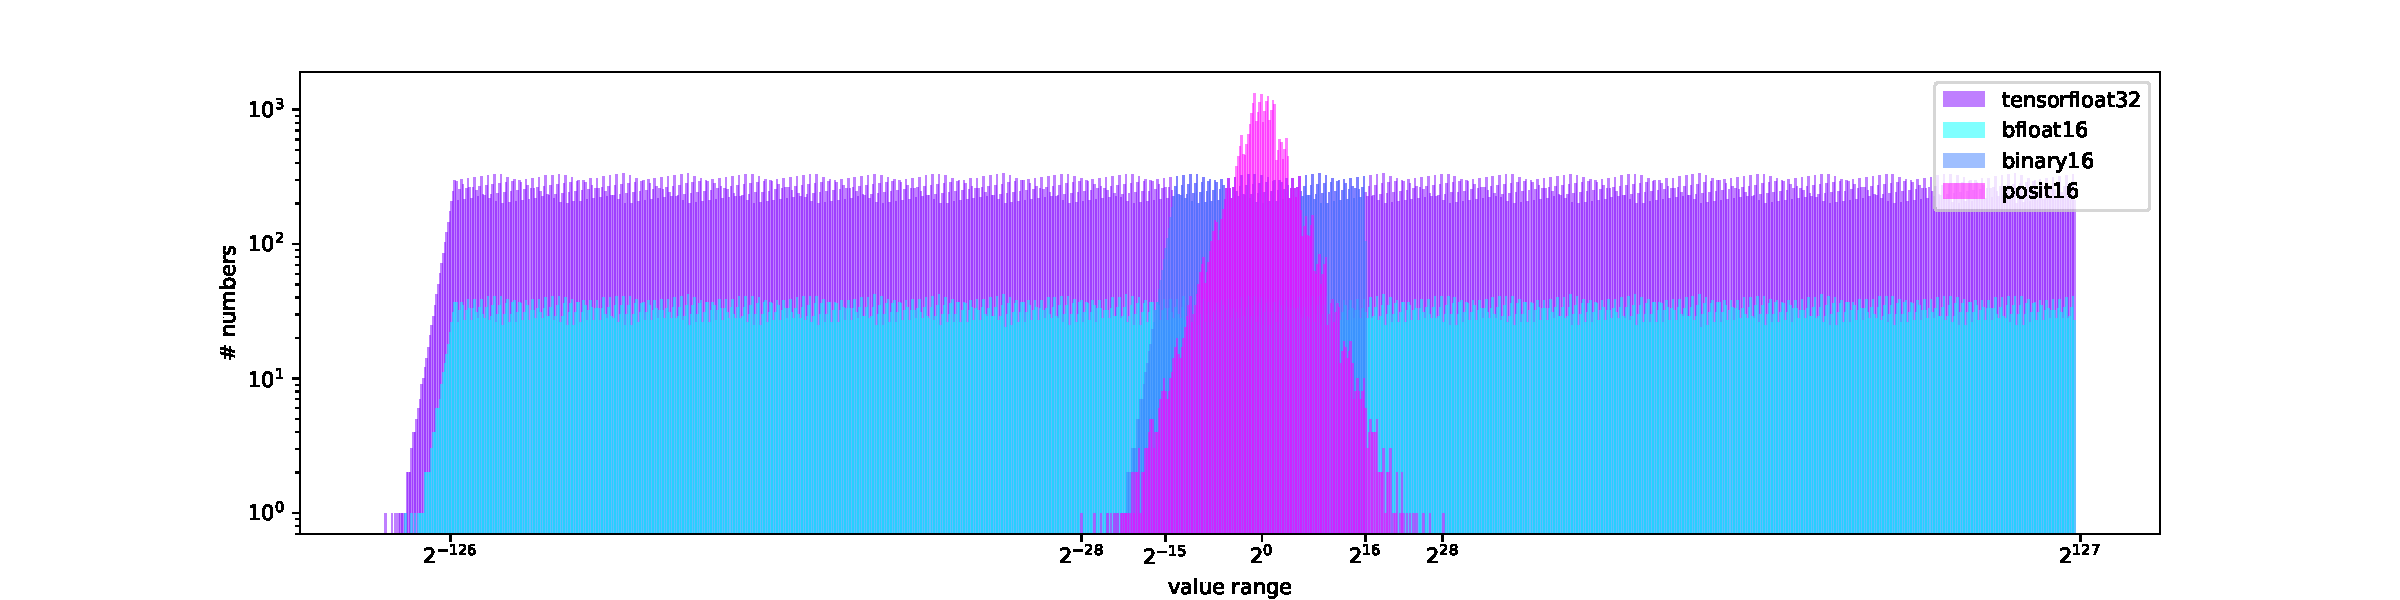
\includegraphics[width=1.0\textwidth]{plots/number_line}
    \caption{Density or distribution of numbers for \gls{tensorfloat32}, \gls{binary16}, \gls{posit16} and \gls{bfloat16}. The number of bins was chosen to be \num{1024} of logarithmic width. The IEEE conformant floats \gls{tensorfloat32}, \gls{binary16} and \gls{bfloat16} exhibit a similar shape, namely the distribution of numbers is exponential decreasing for higher and smaller numbers. The high numbers undergo a rough cutoff at the highest representable number. Numbers above that value will be cast to infinity. Compared to this, the small numbers show a smooth cutoff, because of the existence subnormal numbers. The range of \gls{posit16} is bigger than the range of \gls{binary16}, but specially in the very small numbers this difference in range is negligible. Some features of posits can be observed: First, their distribution is symmetric around \num{1}, because posits have no subnormals. Second, more numbers are closer to \num{1} than in case of floats; the closer to \num{1}, the better the number resolution. Closest to \num{1}, the number resolution becomes better than \gls{binary16} resolution. Third, posits have no fixed-length mantissa nor exponent. That's the reason why the height of the posit shape depends on the number regime, which happens for floats only in the subnormal regime, where the exponent and mantissa are indeed of variable length. For all formats, the amount of numbers decreases exponentially when going away from \num{1}, but posits decrease faster. This suggests that when calculating in the number regime close to \num{1} posits might be the better choice, but when numbers span the whole number range equally, floats might be superior. But in that case one has to take care about over- and underflows. Notice that the height of the shape is determined by the number of mantissa bits, therefore giving the precision, whereas the width is determined by the number of exponent bits, therefore giving the number range. For example \gls{tensorfloat32} and \gls{binary16} have a very different number range, but exhibit the same precision for numbers in their intersection, meaning that \gls{binary16} is a subset of \gls{tensorfloat32}. On the other hand comparing \gls{tensorfloat32} and \gls{bfloat16} they have approximately the same number range, but different precisions in them, meaning that \gls{bfloat16} is as well a subset of \gls{tensorfloat32}, which itself is a subset of \gls{binary32}. Notice that when plotting \gls{binary32} and \gls{posit32} in such a plot, they would look very similar to \gls{binary16} versus \gls{posit16}.}
    \label{fig:number_line}
\end{figure}

\subsection{Floating point numbers in openQxD}

To explore how the conjugate gradient kernel in openQxD would perform when using smaller bit lengths, one can look at the exponentials of the numbers in the matrix and vectors, see Figure \ref{fig:exponents}. The plot shows all exponents appearing together with their overall occurrence in percent. The number zero was taken from the plot, because it has biased exponent $E=-127$. The occurrences for zero are given in the legend.

The highest exponent in all 4 runs was $E=4$, whereas the lowest exponent deceased when the number of lattice points increased. The range of exponents that is representable in \gls{binary16} spans from \textcolor{corange}{$-24$} to \textcolor{cpink}{$+16$} and is indicated by the \textcolor{corange}{solid orange line} and the \textcolor{cpink}{solid pink line}. Between \textcolor{corange}{$-24$} and \textcolor{cblue}{$-14$} is the regime of subnormal numbers in \gls{binary16}, with the lowest regular (non-subnormal) exponent indicated by the \textcolor{cblue}{solid blue line}. When using half precision instead of single precision, all numbers with exponents below \textcolor{corange}{$-24$}, will be converted to zero, whereas exponents above \textcolor{cpink}{$+16$} will be cast to $\pm \infty$ depending on the sign of the number. It can be seen, that when calculating the norm of these numbers, only numbers between the \textcolor{cblue}{dashed blue line} and the \textcolor{cpink}{dashed pink line} will participate. If there is a number above the dashed pink line in the \textcolor{cyellow}{unsafe region} this number will - after squaring - be cast to $\infty$ and therefore the norm will be $\infty$ as well\footnotemark. In this case the variable representing the norm $x = \norm{\vec{v}}$ should be of higher precision than \gls{binary16}. The plot shows that the Dirac matrix \code{Dop()} is confined in a narrow exponent regime and a representation in 16-bit floats would suffice. Notice the sparsity the Dirac matrix.

\footnotetext{A method to circumvent this is to scale the vector entries during the calculation and scale the result back, exploiting homogeneity of the norm, $\norm{\vec{v}} = \frac{1}{s}\norm{s\vec{v}}$ for $s \in \mathbb R_{> 0}$.}

\begin{figure}
    \centering
    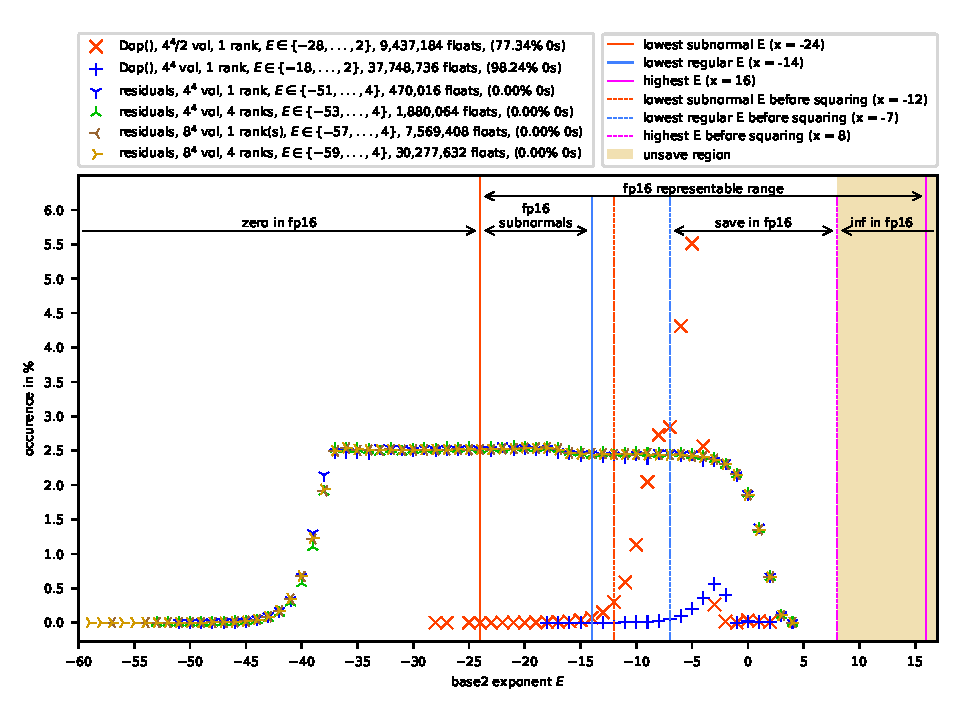
\includegraphics[width=1.0\textwidth]{plots/exponents_dirac}
    \caption{Exponent distribution of \gls{binary32} single precision floats in the residual vectors of all steps in a conjugate gradient run in openQxD as well as entries of the Dirac operator. 4 runs were made, with a lattice size of $4^4$ and $8^4$ on one single rank and $4$ ranks respectively. The number is normalised to $(-1)^s \cdot M \cdot 2^{E}$, where $M \in [1, 2)$.}
    \label{fig:exponents}
\end{figure}


\section{Conjugate Gradient algorithm}

In many scientific computations large systems of linear equations need to be solved. Usually these systems are huge and the matrices and vectors are distributed among many \glspl{rank}. The method to solve such systems should therefore be iterative. The problem can be formulated mathematically in the following way.

\subsection{Derivation}

Let $n \in \mathbb{N}$ and let $A$ be a $n \times n$-matrix with components in $\mathbb{C}$, Hermitian, positive definite and \glslink{sparse matrix}{sparse}

\begin{align*}
    A^{\dagger} &= A, &\text{(\df{Hermitian})} \\
    \forall \vec{x} \in \mathbb{C}^n \setminus \{0\} \quad \colon \quad \vec{x}^{\dagger} A \vec{x} &> 0, &\text{(\df{positive definite})}
\end{align*}

as well as $\vec{b} \in \mathbb{C}^n$ be given, then the \df{system of linear equations} can be described as

\begin{align}
    A \vec{x} = \vec{b}. \label{eq:Axb}
\end{align}

We are interested in the \df{solution} vector $\vec{x}$, that is the one that satisfies the above equation, $n$ is called the \df{problem size}. First let us define a function that will be helpful in the next sections.

\begin{definition}[Quadratic form]

The \df{quadratic form} depends on the problem matrix $A$ as well as on the \df{source} vector $\vec{b}$ and is defined as

\begin{align*}
    f(\vec{x}) = \frac{1}{2} \vec{x}^{\dagger} A \vec{x} - \vec{b}^{\dagger} \vec{x} + c,
\end{align*}

where $c \in \mathbb{C}$. When taking the derivative of this function with respect to $\vec{x}$, we find that

\begin{align*}
    f'(\vec{x}) = A \vec{x} - \vec{b}.
\end{align*}

Therefore finding the extrema of $f(\vec{x})$ is equivalent to solving the linear system of equations \eqref{eq:Axb}. The question whether the solution $\vec{x}$ is unique remains.

\end{definition}

\begin{figure}
    \centering
    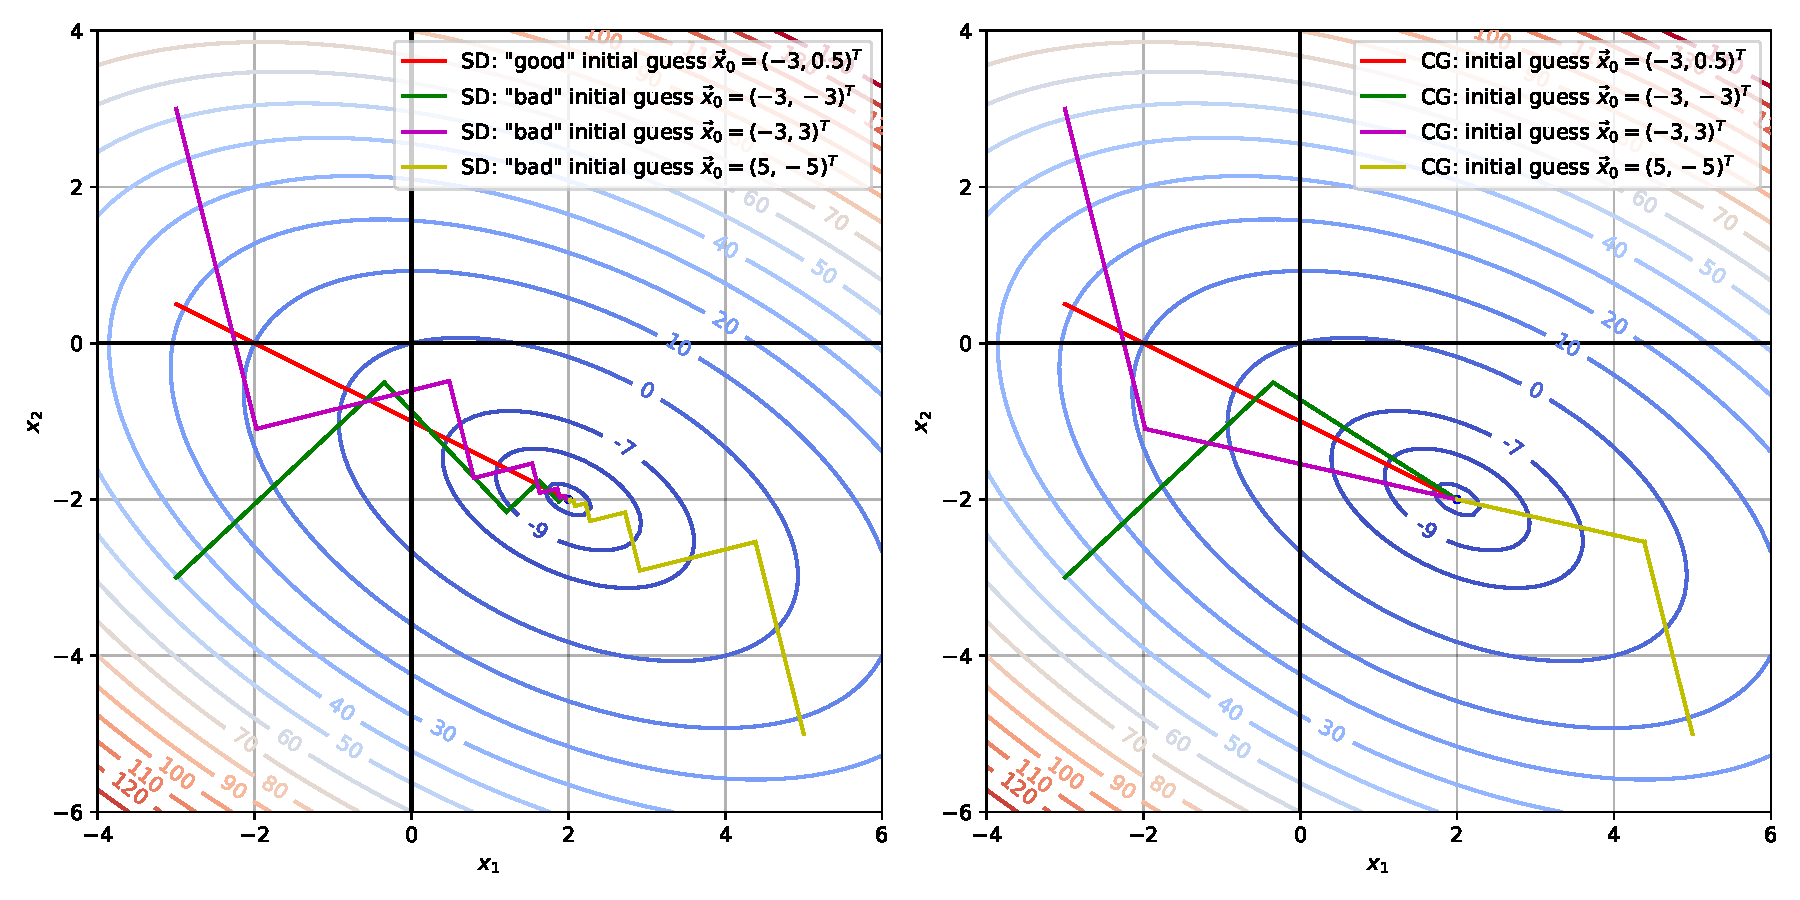
\includegraphics[width=8cm]{plots/qform_contour}
    \caption{Quadratic form TODO}
    \label{fig:qform}
\end{figure}

\begin{lemma}[Uniqueness of the solution]
The solution $\vec{x}$ in equation \eqref{eq:Axb} is unique and the global minimum of $f(\vec{x})$ if $A$ is Hermitian and positive definite \footnotemark.
\end{lemma}

\footnotetext{Notice that, negative definiteness is sufficient as well and $\vec{x}$ would be the global maximum instead - just define $A^{\prime} = -A$ which is positive definite and all of the argumentation that follows will hold as well. Indefinite matrices on the other hand might have local minima and maxima.}

\begin{proof}
Let us rewrite $f(\vec{p})$ at an arbitrary point $\vec{p} \in \mathbb{C}$ in terms of the solution vector $\vec{x}$:

\begin{align*}
    f(\vec{p}) = f(\vec{x}) + \frac{1}{2} (\vec{p} - \vec{x})^{\dagger} A (\vec{p} - \vec{x}). \numberthis \label{eq:fp_cgne}
\end{align*}

This is indeed the same as $f(\vec{p})$ (inserting $A \vec{x} = \vec{b}$ and using $A^{\dagger}=A$ and of $\vec{a}^{\dagger} \vec{b} = \vec{b}^{\dagger} \vec{a}$),

\begin{align*}
f(\vec{x}) + \frac{1}{2} (\vec{p} - \vec{x})^{\dagger} A (\vec{p} - \vec{x}) &= \frac{1}{2} \vec{x}^{\dagger} A \vec{x} - \vec{b}^{\dagger} \vec{x} + c + \frac{1}{2} \vec{p}^{\dagger} A \vec{p} - \frac{1}{2} \vec{p}^{\dagger} A \vec{x} - \frac{1}{2} \vec{x}^{\dagger} A \vec{p} + \frac{1}{2} \vec{x}^{\dagger} A \vec{x} \\
&= \frac{1}{2} \vec{p}^{\dagger} A \vec{p} + c + \vec{x}^{\dagger} \vec{b} - \vec{b}^{\dagger} \vec{x} - \vec{b}^{\dagger} \vec{p} \\
&= \frac{1}{2} \vec{p}^{\dagger} A \vec{p} - \vec{b}^{\dagger} \vec{p} + c \\
&= f(\vec{p}).
\end{align*}

In the new form of $f(\vec{p})$, one can directly see that if $A$ is positive definite, $\vec{x}$ must minimise the function:

\begin{align*}
    f(\vec{p}) = f(\vec{x}) + \frac{1}{2} \underbrace{ (\vec{p} - \vec{x})^{\dagger} A (\vec{p} - \vec{x}) }_{\text{$> 0$ if $A$ pos. def.}}.
\end{align*}

Therefore $\vec{x}$ is the global unique minimum.

\end{proof}

TODO: figure of a pos/neg definite quadratic form.

Before deriving the conjugate gradient method, we look at a related method called the \df{method of steepest descent}. We are interested in a method that iteratively solves equation \eqref{eq:Axb} starting at a \df{initial guess} $\vec{x}_0$ until the series is interrupted, because the approximate solution $\vec{x}_i$ might be close to the real solution by a certain tolerance or the solution was found exactly,

\begin{align*}
    \vec{x}_0 \longrightarrow \vec{x}_1 \longrightarrow \dotsb \longrightarrow \vec{x}_i \longrightarrow \vec{x}_{i+1} \longrightarrow \dotsb
\end{align*}

For each step, we can define the \df{error} and \df{residual} of the current step $i$.

\begin{definition}[Error and Residual]

Define the \df{error} $\vec{e}_i$ and the \df{residual} $\vec{r}_i$ as

\begin{subequations}
    \begin{align}
        \vec{e}_i &= \vec{x}_i - \vec{x}, \label{eq:error} \\
        \vec{r}_i &= \vec{b} - A \vec{x}_i. \label{eq:residual}
    \end{align}
\end{subequations}

\end{definition}

The residual is the vector of discrepancies and the same as $\vec{r}_i = -f'(\vec{x}_i) = -A \vec{e}_i$, the negative derivative of the quadratic form. The derivative point in direction of the maximum increase, thus the residual points in direction of the steepest descent seen from the position of point $\vec{x}_i$.

\begin{definition}[Method of Steepest Descent]
The iteration step equation of the \df{method of steepest descent} in defined as

\begin{align}
    \vec{x}_{i+1} = \vec{x}_i + \alpha_i \vec{r}_i \label{eq:steepest_descent},
\end{align}

where the $\alpha_i \in \mathbb{C}$ are the amounts to go in direction $\vec{r}_i$. The $\alpha_i$ are determined by minimising the parabola with respect to $\alpha_i$, $\frac{d}{d \alpha_i} f(\vec{x}_{i+1}) \stackrel{!}{=} 0$.

\end{definition}

TODO: figure of steepest descent zigzag.

\begin{remark}[Convergence]
As seen in figure [TODO], the method of steepest descent converges very slowly to the actual solution, when starting at an unfavourable starting point $\vec{x}_0$. The speed of convergence also heavily depends on the condition number of matrix $A$. We see that the iteration goes in the same direction multiple times. How about, when we only go \textit{once} in each direction $i$, but by the perfect amount $\alpha_i$? Then we would be done after at most $n$ steps.
\end{remark}

This gives motivation for a enhanced method. Let's define a new \df{step equation} as

\begin{align}
    \vec{x}_{i+1} = \vec{x}_i + \alpha_i \vec{p}_i, \label{eq:cg_step}
\end{align}

with \df{directions} $\vec{p}_i$ and \df{amounts} $\alpha_i$ that have to be determined. But this time, we will impose the condition to go in every direction only once at most. This will lead us to the \df{method of conjugate gradient}.

Using the step equation \eqref{eq:cg_step}, we can update the error and residuals,

\begin{subequations}
    \begin{align}
        \vec{e}_{i+1} &= \vec{x}_{i+1} - \vec{x} \\
                      &= \vec{e}_{i} + \alpha_i \vec{p}_{i} \label{eq:cg_error1} \\
                      &= \vec{e}_{0} + \sum_{j=0}^{i} \alpha_j \vec{p}_{j}, \label{eq:cg_error2}
    \end{align}
\end{subequations}

\begin{subequations}
    \begin{align}
        \vec{r}_{i+1} &= \vec{b} - A \vec{x}_{i+1} \label{eq:residual_exact} \\
                      &= \vec{r}_{i} - \alpha_i A \vec{p}_{i} \label{eq:residual_recursive} \\
                      &= - A \vec{e}_{i+1}. \label{eq:residual_exact2}
    \end{align}
\end{subequations}

The $\{\vec{p}_i\}$ need to form a basis of $\mathbb{C}^n$, because the method should succeed with any arbitrary initial guess $\vec{x}_0$. Since we move in the vector space $\mathbb{C}^n$ from an arbitrary point $\vec{x}_0$ to the solution $\vec{x}$, the $n$ direction vectors need cover all possible directions in the space, therefore need to be linear independent.

To be done after at most $n$ steps, we need that the $n$-th error is zero, $\vec{e}_n = 0$. Since the directions form a basis, we can write $\vec{e}_0$ as a linear combination of the $\{\vec{p}_i\}$,

\begin{align*}
    \vec{e}_{0} = \sum_{j=0}^{n-1} \delta_j \vec{p}_j.
\end{align*}

Using this we can rewrite $\vec{e}_n$,

\begin{align*}
    \vec{e}_{n} &= \vec{e}_o + \sum_{j=0}^{n-1} \alpha_j \vec{p}_j \\
                &= \sum_{j=0}^{n-1} \delta_j \vec{p}_j + \sum_{j=0}^{n-1} \alpha_j \vec{p}_j \\
                &= \sum_{j=0}^{n-1} (\delta_j + \alpha_j) \vec{p}_j.
\end{align*}

In order for this to be zero, all coefficients need to be zero, thus $\delta_j = - \alpha_j$. Then the $i$-th error can be written in a different way

\begin{align*}
    \vec{e}_{i} &= \vec{e}_0 + \sum_{j=0}^{i-1} \alpha_j \vec{p}_j \\
                &= \sum_{j=0}^{n-1} \delta_j \vec{p}_j - \sum_{j=0}^{i-1} \delta_j \vec{p}_j \\
                &= \sum_{j=i}^{n-1} \delta_j \vec{p}_j. \numberthis \label{eq:error_i}
\end{align*}

In the last row, we can see that after every step in the iteration, we shave off the contribution of one direction $\vec{p}_i$ to the initial error $\vec{e}_0$ (or phrased differently: $\vec{e}_{i+1}$ has no contribution from direction $\vec{p}_i$). But we still need to find these directions. We could for example impose that the $(i+1)$-th error should be orthogonal to the $i$-th direction, because we never want to go in that direction again,

\begin{align*}
    0 &\stackrel{!}{=} \vec{p}_i^{\dagger} \vec{e}_{i+1} \\
                    &= \vec{p}_i^{\dagger} ( \vec{e}_{i} + \alpha_i \vec{p}_i ).
\end{align*}

This gives us a expression for the amount $\alpha_i$,

\begin{align*}
    \alpha_i = - \frac{ \vec{p}_i^{\dagger} \vec{e}_{i} }{ \vec{p}_i^{\dagger} \vec{p}_i }.
\end{align*}

The problem with this expression is that we don't know the value of $\vec{e}_i$ - if we would, we could just subtract it from the current $\vec{x}_i$ and obtain $\vec{x}$ exactly. So, we do not know $\vec{e}_i$, but what we actually know is something similar, namely $-A \vec{e}_i$, with is the residual. So if we manage to sandwich an $A$ in the expression above, we are save. It turns out that imposing $A$-orthogonality instead of regular orthogonality between $\vec{e}_{i+1}$ and $\vec{p}_i$ achieves what we're up to by the exact same steps\footnotemark,

\begin{align*}
    0 &\stackrel{!}{=} \vec{p}_i^{\dagger} A \vec{e}_{i+1} \\
                    &= \vec{p}_i^{\dagger} A ( \vec{e}_{i} + \alpha_i \vec{p}_i ) \\
\end{align*}

\footnotetext{This is equivalent to imposing $0 \stackrel{!}{=} \vec{r}_{i+1}^{\dagger} \vec{p}_i$ which is done in most literature, but in the opinion of the author this is less intuitive.}

Solving for $\alpha_i$ gives the (almost) final expression for the amounts,

\begin{align}
      \implies         \alpha_i &= - \frac{ \vec{p}_i^{\dagger} A \vec{e}_{i} }{ \vec{p}_i^{\dagger} A \vec{p}_i } = \frac{ \vec{p}_i^{\dagger} \vec{r}_{i} }{ \vec{p}_i^{\dagger} A \vec{p}_i }. \label{eq:cgne:alpha_pre}
\end{align}

Notice that the denominator is never zero, because $A$ is positive definite. Let us continue with the expression for $A$-orthogonality, but insert the derived expression \eqref{eq:error_i} for $\vec{e}_{i+1}$ this time,

\begin{align*}
    0 &\stackrel{!}{=} \vec{p}_i^{\dagger} A \vec{e}_{i+1} \\
                    &= \vec{p}_i^{\dagger} A \left[ \sum_{j=i+1}^{n-1} \delta_j \vec{p}_j \right] \\
                    &= \sum_{j=i+1}^{n-1} \underbrace{ \delta_j }_{\text{\makebox[0pt]{$\neq 0$} }} \vec{p}_i^{\dagger} A \vec{p}_j.
\end{align*}

This implies that for $j>i$ and $i \in \{0, \dots, n-1\}$, we have

\begin{align*}
    \vec{p}_i^{\dagger} A \vec{p}_j = 0.
\end{align*}

But since $A$ is Hermitian, we can Hermitian conjugate the whole expression above and obtain

\begin{align*}
    0 = \left( \vec{p}_i^{\dagger} A \vec{p}_j \right)^{\dagger} = \vec{p}_j^{\dagger} A \vec{p}_i.
\end{align*}

So the expression holds for $i>j$ as well, which implies that the $\{\vec{p}_i\}$ are \df{$A$-orthogonal},

\begin{align*}
    \vec{p}_i^{\dagger} A \vec{p}_j = 0 \quad \forall i \neq j.
\end{align*}

So the problem has reduced to finding a set of $A$-orthogonal vectors in an iterative way. Luckily there is a well know method to find orthogonal vectors from a set of linear independent vectors: \df{Gram-Schmidt orthogonalization}. The procedure can be altered to find $A$-orthogonal vectors instead.

\begin{definition}[Gram-Schmidt Orthogonalization]

\label{df:gramschmidt}

Let $\{ \vec{u}_0, \dots, \vec{u}_{n-1} \} \subset \mathbb{C}^n$ be a set of $n$ linear independent vectors. The iterative Gram-Schmidt procedure is

\begin{align}
    \begin{split}
        \vec{p}_0 &= \vec{u}_0 \label{eq:gramschmidt} \\
        \vec{p}_i &= \vec{u}_i + \sum_{k=0}^{i-1} \beta_{ik} \vec{p}_k,
    \end{split}
\end{align}

where the $\beta_{ik} \in \mathbb{C}$ are (to be determined) coefficients. In the regular procedure, the $\beta_{ik}$ are just normalised projections of $\vec{u}_i$ to $\vec{p}_k$ that are subtracted from $\vec{u}_i$, leading to a vector $\vec{p}_i$ that is orthogonal to all previously calculated $\vec{p}_k$.

\end{definition}

In our problem, we need a set of vectors that are $A$-orthogonal. By imposing this condition we find a different expression for the $\beta_{ik}$,

\begin{align*}
    0 &\stackrel{!}{=} \vec{p}_i^{\dagger} A \vec{p}_j \\
                    &= \vec{u}_i^{\dagger} A \vec{p}_j + \sum_{k=0}^{i-1} \beta_{ik} \vec{p}_k^{\dagger} A \vec{p}_j \\
                    &= \vec{u}_i^{\dagger} A \vec{p}_j + \beta_{ij} \vec{p}_j^{\dagger} A \vec{p}_j,
\end{align*}

where in the last step, we assumed $i>j$ (else we would not find a expression for $\beta_{ij}$) and therefore only the $j$-th term in the sum remains, because of the $A$-orthonormality of the directions. Solving this for $\beta_{ij}$ gives

\begin{align}
    \beta{ij} = - \frac{ \vec{u}_i^{\dagger} A \vec{p}_j }{ \vec{p}_j^{\dagger} A \vec{p}_j }. \label{eq:betas}
\end{align}

In principle we are done here, we only need a set of linearly independent vectors $\{\vec{u}_i\}$. Since the conjugate gradient method is iterative and often dealing with huge problem sizes $n$, we need to store all previous directions $\vec{p}_k$ in order to calculate the current direction (see equation \eqref{eq:gramschmidt}). This becomes a problem in limited memory situations. We want that the current step only depends on the previous one. By imposing this condition, we need the sum in equation \eqref{eq:gramschmidt} to collapse; the $\beta_{ik}$ should only be non-zero for $k=i-1$. If we manage to satisfy this, the orthogonalization procedure would simplify to

\begin{align*}
    \beta_i &\coloneqq \beta_{i, i-1}, \\
    \vec{p}_i &= \vec{u}_i + \beta_i \vec{p}_{i-1},
\end{align*}

where in the second equation, the current $\vec{p}_i$ only depends on the previous $\vec{p}_{i-1}$. For this to hold, all other $\beta_{ij}$ need to be zero. For such a $\beta_{ij}$ the numerator needs to be zero. Let therefore $j<i-1$

\begin{align*}
    \vec{u}_i^{\dagger} A \vec{p}_j &\stackrel{!}{=} 0.
\end{align*}

To find a different expression for the left hand side, consider

\begin{align*}
    \vec{u}_i^{\dagger} \vec{r}_{j+1} &= \vec{u}_i^{\dagger} \left( \vec{r}_j + \alpha_j A \vec{p}_j \right) \\
    &= \vec{u}_i^{\dagger} \vec{r}_j + \alpha_j \textcolor{cyellow}{\vec{u}_i^{\dagger} A \vec{p}_j}, \\
    \implies \textcolor{cyellow}{\vec{u}_i^{\dagger} A \vec{p}_j} &= \frac{1}{\alpha_j} \left[ \vec{u}_i^{\dagger} \vec{r}_{j+1} - \vec{u}_i^{\dagger} \vec{r}_j \right], \numberthis \label{eq:uiAdj}
\end{align*}

where we inserted the recursive relation of the residuals \eqref{eq:residual_recursive} and the \textcolor{cyellow}{yellow} part is the expression we want to be \textcolor{cyellow}{zero} for $j<i-1$. We therefore find a condition for the linear independent set $\{\vec{u}_i\}$, namely that the scalar product of $\vec{u}_i$ with $\vec{r}_{j+1}$ and $\vec{r}_{j}$ must be the same. But we can apply the same equation over and over again and obtain

\begin{align*}
    \vec{u}_i^{\dagger} \vec{r}_{j+1} &= \vec{u}_i^{\dagger} \vec{r}_j = \dots = \vec{u}_i^{\dagger} \vec{r}_0, &j<i-1
\end{align*}

We have to find $\{\vec{u}_i\}$ that satisfy the above equation. It is sufficient to find a set of $\{\vec{u}_i\}$ that are orthogonal to all the residuals and the equation would be obeyed.

\begin{lemma}[]
\label{lem:rorthogonality}
The residuals are orthogonal, thus for all $i \neq j$, it holds

\begin{align*}
    \vec{r}_i^{\dagger} \vec{r}_j = 0.
\end{align*}

\end{lemma}

\begin{proof}

The proof consists of 2 steps.

\begin{enumerate}[label={\arabic*)}]
    \item Let $i<j$,

    \begin{align*}
        \vec{p}_i^{\dagger} \vec{r}_j &= - \vec{p}_i^{\dagger} A \vec{e}_j \\
                                      &= - \sum_{k=j}^{n-1} \delta_j \textcolor{cyellow}{\vec{p}_i A \vec{p}_k} \\
                                      &= 0,
    \end{align*}

    where the \textcolor{cyellow}{yellow} expression is \textcolor{cyellow}{zero}, because $i<j\leq k$.

    \item Let $i<j$. By step 1), we have

    \begin{align*}
        0 &= \vec{p}_i^{\dagger} \vec{r}_j \\
          &= \vec{r}_i^{\dagger} \vec{r}_j + \sum_{k=0}^{i-1} \beta_{ik} \textcolor{cyellow}{\vec{p}_k^{\dagger} \vec{r}_j} \\
          &= \vec{r}_i^{\dagger} \vec{r}_j.
    \end{align*}

    The \textcolor{cyellow}{yellow} expression is again \textcolor{cyellow}{zero} by step 1). Using the symmetry of the scalar product, the above equation also holds for $i$ and $j$ interchanged ($i>j$), therfore holds for all $i \neq j$.

\end{enumerate}

\end{proof}

From now on we set $\vec{u}_i = \vec{r}_i$. What remains to find is the final expression for the $\beta_i$.

\begin{align*}
    \beta_i \coloneqq \beta_{i,i-1} &= - \frac{ \vec{u}_i^{\dagger} A \vec{p}_{i-1} }{ \vec{p}_{i-1}^{\dagger} A \vec{p}_{i-1} } \\
    &= - \frac{1}{\vec{p}_{i-1}^{\dagger} A \vec{p}_{i-1} } \frac{1}{\alpha_{i-1}} \left[ \vec{r}_i^{\dagger} \vec{r}_i - \textcolor{cyellow}{\vec{r}_i^{\dagger} \vec{r}_{i-1}} \right] \\
    &= - \frac{ \vec{r}_i^{\dagger} \vec{r}_i }{ \alpha_{i-1} \vec{p}_{i-1}^{\dagger} A \vec{p}_{i-1} } \\
    &= - \frac{ \vec{r}_i^{\dagger} \vec{r}_i }{ \vec{p}_{i-1}^{\dagger} \vec{r}_{i-1} },
\end{align*}


where in the first row we used the definition \eqref{eq:betas}, in the second row we have used equation \eqref{eq:uiAdj} and the \textcolor{cyellow}{yellow} expression is \textcolor{cyellow}{zero} by the orthogonality of the residuals lemma \ref{lem:rorthogonality}. In the last line we used the expression for the $\alpha_j$ equation \eqref{eq:cgne:alpha_pre}

To obtain the final form of the $\alpha_i$ and the $\beta_i$, we can use a leftover of the proof of lemma \ref{lem:rorthogonality}, namely

\begin{align*}
    \vec{p}_i^{\dagger} \vec{r}_i &= \vec{r}_i^{\dagger} \vec{r}_i + \beta_i \underbrace{\textcolor{cyellow}{\vec{p}_{i-1}^{\dagger} \vec{r}_i}}_{ \mathrlap{\text{$=0$ by lemma \ref{lem:rorthogonality} step 1) }} } \\
    &= \vec{r}_i^{\dagger} \vec{r}_i.
\end{align*}


Using this we find the final form of the $\alpha_i$ and the $\beta_i$ as well as the \df{method of conjugate gradient}.

\begin{definition}[Method of conjugate gradient]

The iteration step equation of the \df{method of conjugate gradient} in defined as

\begin{align*}
    \vec{x}_{i+1} = \vec{x}_i + \alpha_i \vec{p}_i,
\end{align*}

with

\noindent\begin{minipage}{.5\linewidth}
    \begin{align*}
        \vec{r}_{i+1} &= \vec{r}_{i}   - \alpha_i A  \vec{p}_i, \\
        \vec{p}_{i+1} &= \vec{r}_{i+1} + \beta_{i+1} \vec{p}_i, 
    \end{align*}
\end{minipage}
\begin{minipage}{.5\linewidth}
    \begin{align}
        \alpha_i    &=   \frac{ \vec{r}_{i}^{\dagger} \vec{r}_{i} }{ \vec{p}_i^{\dagger} A \vec{p}_i }, \label{eq:alphai} \\
        \beta_{i+1} &= - \frac{ \vec{r}_{i+1}^{\dagger} \vec{r}_{i+1} }{ \vec{r}_{i}^{\dagger} \vec{r}_{i} }, \label{eq:betai}
    \end{align}
\end{minipage}

and initial starting vectors

\begin{align*}
    \vec{x}_{0} &= \text{arbitrary starting point}, \numberthis \label{eq:cg:start} \\
    \vec{p}_{0} &= \vec{r}_{0} = \vec{b} - A \vec{x}_0.
\end{align*}

\end{definition}

There are some remarks to note about the method of conjugate gradient.

\begin{remark}
    The $\beta_{i+1}$ of the current iteration depends on the norm of the current residual as well as the last one. This means that we can store the result of the last iteration and reuse it in the current, the norm may not be calculated twice.
\end{remark}

\begin{remark}
    In the source code of openQxD (see \cite{openqxd}) the matrix $A$ is the Dirac matrix applied twice $A = D^{\dagger} D$. This means that the denominator of $\alpha_i$ is a regular inner product as well; $\vec{p}_i^{\dagger} A \vec{p}_i = \vec{p}_i^{\dagger} D^{\dagger} D \vec{p}_i = \left( D \vec{p}_i \right)^{\dagger} \left( D \vec{p}_i \right) = \norm{ D \vec{p}_i }^2$
\end{remark}

\begin{remark}
    Therefore in each iteration, we have:
    \begin{itemize}
        \item 2 times the norm of a vector,
        \item 2 matrix-vector multiplications,
        \item 3 times axpy.\footnotemark
    \end{itemize}
\end{remark}

\begin{remark}[Floating point errors]
    Since the method contains recursive steps, floating point round-off accumulation is an issue. This causes the residuals to loose their $A$-orthogonality. It can be resolved by calculating the residual from time to time using its (computationally more expensive) definition $\vec{r}_i = \vec{b} - A \vec{x}_i$, which involves one matrix vector multiplication. One can for example do this every $m$-th step. The same problem applies to the directions $\vec{p}_i$ that loose their $A$-orthogonality.
\end{remark}

\begin{remark}[Problem size]
    The method of conjugate gradient is suitable for problems of very huge size $n$. The algorithm is done after $n$ steps, but there might be problems such that even $n$ steps are out of reach for an exact solution.
\end{remark}

\begin{remark}[Complexity]
    The time complexity of the conjugate gradient method is $O(m \sqrt{\kappa})$, where $m$ is the number of non-zero entries in $A$ and $\kappa$ is its \df{condition number}. The space complexity is $O(m)$.
\end{remark}

\begin{remark}[Starting]
    The \df{starting vector} $\vec{x}_0$ can be chosen at wish. If there is already a rough estimate of the solution one can take that vector. But usually just $\vec{x}_0 = 0$ is chosen. Since the minimum is global, there is no issue in choosing a starting point. The method will always converge towards the real solution.
\end{remark}

\begin{remark}[Stopping]
    If the problem size does not allow to run $n$ steps, one can stop when the norm of the residual falls below a certain \df{threshold} value. Usually this threshold is a fraction of the initial residual $\norm{\vec{r}_i} < \epsilon \norm{\vec{r}_0}$ \cite{shewchuk1994}.
\end{remark}

\begin{remark}[Initialisation]
    The very first step of the method is equivalent to a step in the method of steepest descent, see equation \eqref{eq:steepest_descent}.
\end{remark}

\begin{remark}[Speed of convergence]
    TODO: cg is quicker if there are duplicated eigenvalues. number of iterations for exact solution is at most the number of distinct eigenvalues.
\end{remark}

\begin{remark}[Preconditioning]
    The linear system of equations can be transformed using a matrix $M$ to

    \begin{align*}
        M^{-1} A \vec{x} = M^{-1} \vec{b}.
    \end{align*}

    It is assumed $M$ is such that it is easy to invert and it approximates $A$ in some way, resulting in $M^{-1} A$ to be better conditioned than $A$\footnote{Or stated differently, that $M^{-1}A$ has a more clustered spectrum than $A$.}. An example of a particular preconditioner $M$ would be a diagonal matrix, with diagonal entries of $D$. It is indeed easy to invert and it approximates $A$ quite well if $A$ has non-zero diagonal entries and most off-diagonal entries are zero.
\end{remark}

\begin{remark}[\acrfull{cgne}]
    The algorithm can be used even if $A$ is not symmetric nor Hermitian nor positive definite. The linear system of equations to be solved is then

    \begin{align*}
        A^{\dagger} A \vec{x} = A^{\dagger} \vec{b}.
    \end{align*}

    If $A$ is square and invertible, solving the above equation is equivalent to solving $A \vec{x} = \vec{b}$. Conjugate gradient can be applied, because $A^{\dagger} A$ is Hermitian and positive ($\vec{x}^{\dagger} A^{\dagger} A \vec{x} = \norm{A \vec{x}} \ge 0$). Notice that $A^{\dagger} A$ is less sparse than $A$, and often $A^{\dagger} A$ is badly conditioned.

\end{remark}

\footnotetext{This stands for $a \vec{x} + \vec{y}$, scalar times vector plus vector, "a x plus y" (to resemble the \acrshort{BLAS} level 1 routine call of the same name).}

\subsection{CG kernel in openQxD}

\label{sec:fp_in_openqxd}

The conjugate gradient kernel \code{cgne()} in \code{modules/linsolv/cgne.c} in \cite{openqxd} implements the algorithm, see Listing \ref{lst:cgne}. The algorithm is already implemented in mixed precision using \gls{binary32} in most of the computations and \gls{binary64} in correction steps\footnote{The method is also referred to as \df{mixed precision defect-correction}, see ref. \cite{goddeke2005}}.

\begin{comment}
The disadvantage of defect-correction, however, is that the Krylov search space that is built up is discarded each time the solver is restarted.

Other possibility: "reliable updates" scheme:
\end{comment}

\begin{figure} % wrap into a figure such that the whole snippet is on the same page
\begin{lstlisting}[
    language=C,
    firstnumber=429,
    label=lst:cgne,
    caption={The conjugate gradient kernel in \code{modules/linsolv/cgne.c} line \num{429}ff.}
]
double cgne(int vol,int icom,void (*Dop)(spinor *s,spinor *r),
            void (*Dop_dble)(spinor_dble *s,spinor_dble *r),
            spinor **ws,spinor_dble **wsd,int nmx,double res,
            spinor_dble *eta,spinor_dble *psi,int *status)
{
\end{lstlisting}
\end{figure} 

The function expects the Dirac matrix \code{Dop()} in \gls{binary32}, \code{Dop\_dble()} in \gls{binary64} format and the source vector \code{eta} ($\vec{b}$) in \gls{binary64} only. In the initialisation the starting vector \code{psi} ($\vec{x}_0$) is set to zero. The algorithm stops when the desired maximal relative residue \code{res} ($=\frac{\norm{\code{eta}-D^\dagger D \code{psi}}}{\norm{\code{eta}}}$) is reached, where \code{psi} is the calculated approximate solution of the Dirac equation $D^\dagger D \code{psi}=\code{eta}$ in \gls{binary64}. For this, the tolerance \code{tol} is calculated using $\code{tol} = \norm{\code{eta}} * \code{res}$. The parameter \code{nmx} is the maximal number of iterations that may be applied and \code{status} reports the total number of iterations that were required, or a negative value if the algorithm failed. \code{icom} is a control parameter and \code{ws} and \code{wsd} are work space allocations. The volume of the lattice should be given in \code{vol}.

Since the Dirac matrix is given in two precisions, the algorithm in the code bails out of the main conjugate gradient loop, when some particular conditions where met, see Listing \ref{lst:break}.

\begin{figure} % wrap into a figure such that the whole snippet is on the same page
\begin{lstlisting}[
    language=C,
    firstnumber=490,
    label=lst:break,
    caption={break condition in \code{modules/linsolv/cgne.c} line \num{490}ff, \code{rn} is the norm of the current residual, \code{xn} is the norm of the current solution vector, both in \gls{binary32}.}
]
if ((rn<=tol)||(rn<=(PRECISION_LIMIT*xn))||(ncg>=100)||
    ((*status)>=nmx))
   break;
\end{lstlisting}
\end{figure} 

This may happen in 4 cases:

\begin{enumerate}
  \item if the recursively calculated residual is below the tolerance,
  \item if the precision of \gls{binary32} is reached\footnotemark,
  \item after a hard coded number of \num{100} steps,
  \item if the maximal number of steps is reached.
\end{enumerate}

\footnotetext{The constant \code{PRECISION\_LIMIT} is defined to be \code{100*MACHINE\_EPSILON}, where the \code{MACHINE\_EPSILON} is the difference between \num{1} and the lowest value above \num{1} depending on the datatype. In case of \gls{binary32} the \code{MACHINE\_EPSILON} takes a value of \num[round-mode = figures, round-precision = 8, scientific-notation = true]{1.1920928955078125e-07}.}

Point 2 is the most interesting condition, because lets imagine that this condition is met, but the algorithm does not break out of the main loop. Therefore the norm of the current residual compared to the norm of the current solution vector differ in their orders of magnitude by the precision limit of the datatype (\gls{binary32} in this case). This means that the solution vector $\vec{x_i}$ contains large numbers compared to the residual vector $\vec{r_i}$. Therefore the changing in residual from iteration to iteration is small compared to numbers in $\vec{x_i}$ as well. Since $\vec{r_i}$ contains small numbers, the amounts $\alpha_i$ are small as well. This causes $\vec{x_{i+1}} = \vec{x_i} + \alpha_i \vec{d_i}$ to not change anymore, because adding very large and very small numbers in floating point arithmetic will return the larger number unchanged if the two numbers differ in magnitude by the precision limit of the datatype. The algorithm stalls in that case and breaking out of the main loop is the emergency brake.

So when one of the above conditions are met, the algorithm performs a \df{reset step}. A reset step consists of calculating the residual not in the recursive way, instead calculating it in it's definition $\vec{r_i} = \vec{b} - A \vec{x_i}$ in double precision. This involves \num{2} invocations of each \code{Dop\_dble()} as well as \code{Dop()} which is very expensive. The algorithm is resetting in the sense that the solution vector is set back to $\vec{x_i} = 0$, but before resetting, the solution vector in \gls{binary32} is added to the real solution vector \code{psi} in \gls{binary64} which was initialised to zero at the start of the algorithm as well. It looks like a restart of the whole calculation, but the direction for the next iteration $\vec{d_i} = \vec{r_i}$ is set to the just calculated, very accurate residual. Therefore the the algorithm now continues in a new direction $A$-orthogonal to all previous directions and progression is kept. The step is meant to remove the accumulated round-off errors due to the recursive calculation of the residuals and directions. The first step following a reset step is a step in the direction of steepest descent just like the very first step of the algorithm. The less precise the datatype, the more reset steps need to be taken, because the precision limit is reached earlier.

\subsection{Simulating CG with different datatypes}

\label{sec:simulating_cgne}

Some operations such as norms and scalar products are memory-bandwidth-bound, which means the on-chip memory bandwidth determines how much time is spent computing the output. Storing input data in a format with lower bit-length reduces the amount of data to be transferred, thus improving the speed of calculation.

The complete conjugate gradient kernel was simulated in different datatypes, floats as well as posits. In order to produce the plots, the Dirac matrix \code{Dop\_dble()} and the source vector $\code{eta}$ were extracted in \gls{binary64} format from the original code running a simulation of a $4^4$ lattice, \acrfull{sf} boundary conditions (\code{type 1}), no C* boundary conditions (\code{cstar 0}) and $1$ rank. The first \num{2000} trajectories were considered of thermalisation. The matrix was extracted in trajectory \num{2001}. A python script mimicking the exact behaviour of the \code{cgne()} kernel from the source code\footnotemark, was implemented to cope with arbitrary datatypes. The simulated datatypes were \gls{binary64}, \gls{binary32}, \gls{tensorfloat32}, \gls{binary16}, \gls{bfloat16}, \gls{posit32}, \gls{posit16}, and \gls{posit8}. The Dirac matrix had approximately \num{2}\% non-zero value. The results are plotted in figures \ref{fig:cgne:naive}, \ref{fig:cgne:quire}, \ref{fig:cgne:col64} and \ref{fig:cgne:res12}.

\footnotetext{See line 429ff in \code{modules/linsolv/cgne.c} in \cite{openqxd}.}

\begin{comment}
\begin{figure}
    \centering
    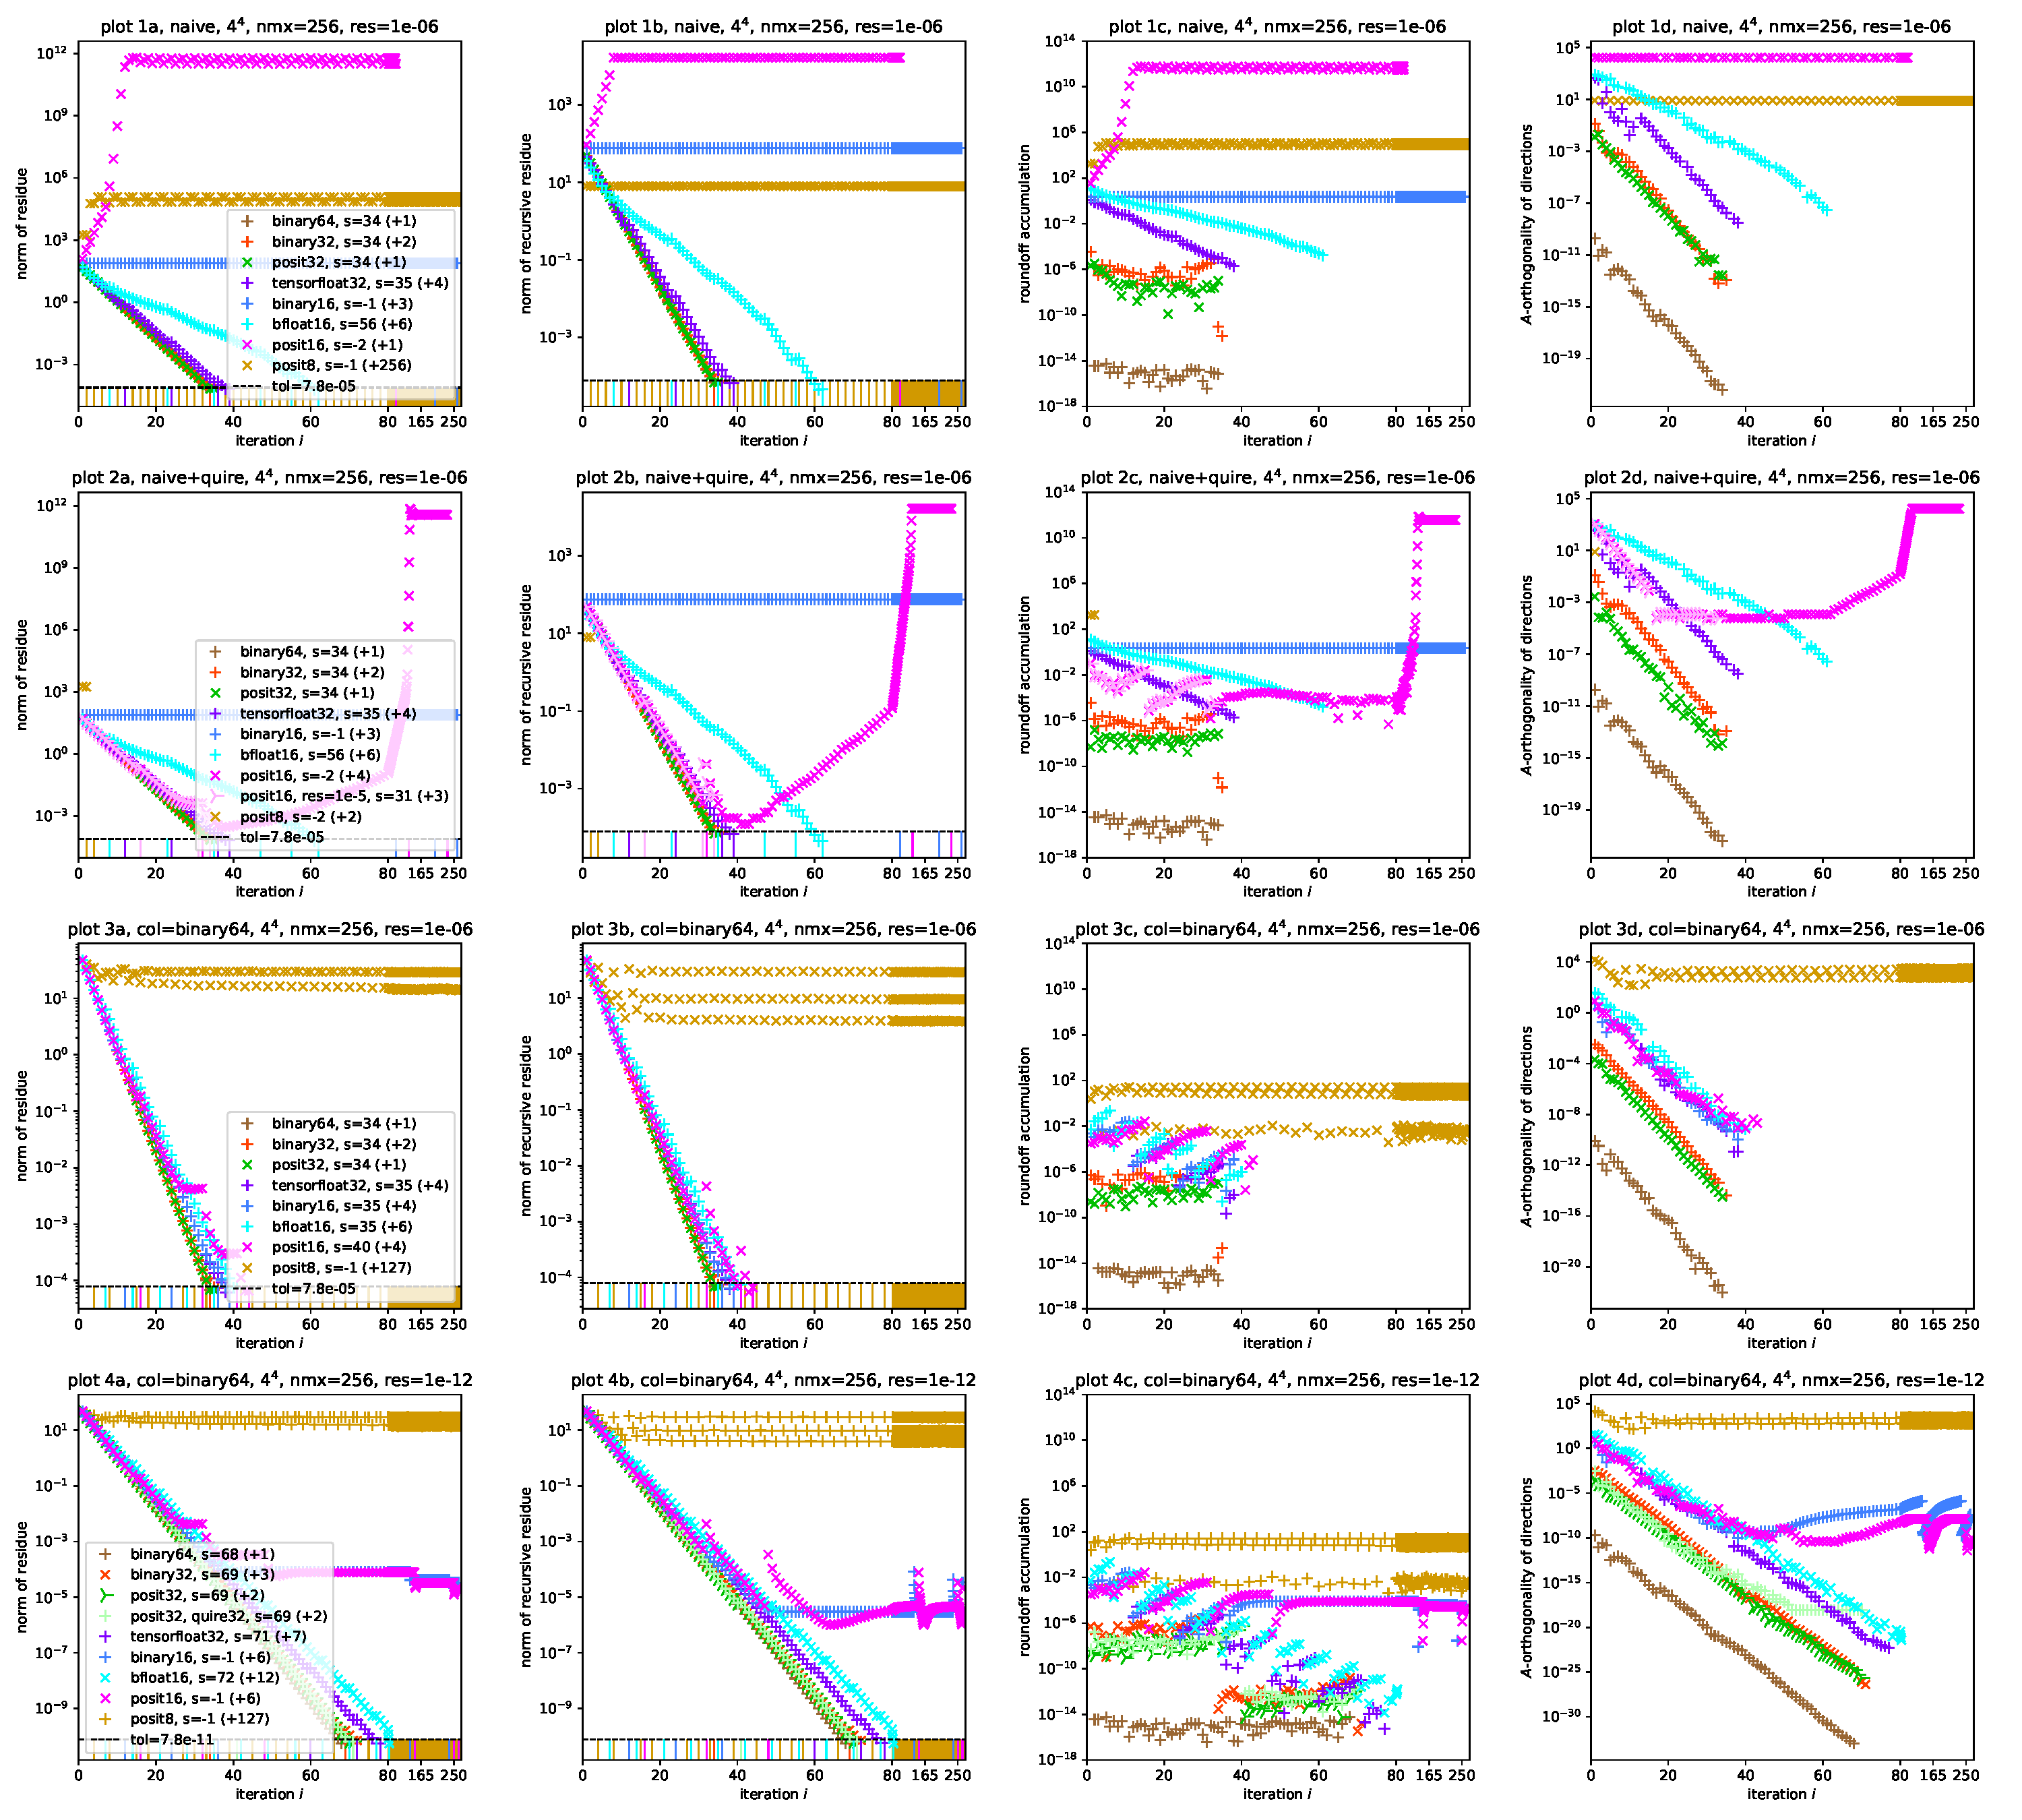
\includegraphics[width=1.0\textwidth]{plots/cgne}
    \caption{Convergence analysis of a conjugate gradient run, where \gls{binary32} was replaced by one of the simulated datatypes. The legend for every row is equal, displayed only in the first plot of the row. The number \code{s} describes the number of normal steps needed (the value of \code{status}), whereas the numbers in the brackets indicates the number of reset steps. All reset steps are indicated by ticks at the dashed black tolerance line. The iterations will always go up to \code{nmx=256}, but the range \num{80}-\num{256} is compressed since the most interesting behaviour happens before step \num{80} for most of the simulated datatypes. The \textit{first row} shows a naive replacement of the \gls{binary32} datatype with the simulated one. This means that every single variable containing a \gls{binary32} was replaced with a variable of the simulated datatype. Plot \textit{1a} shows the exact residue \eqref{eq:residual_exact} in every iteration calculated using the Dirac matrix and the source vector both in \gls{binary64}, whereas plot \textit{1b} shows the norm of the recursively calculated residue \eqref{eq:residual_recursive} (cast after the calculation from the simulated datatype to \gls{binary64}). The relative residue suffers round-off accumulation because of the recursive calculation; this is the difference between plots \textit{1a} and \textit{1b}, which is plotted in plot \textit{1c}. Plot \textit{1d} shows the $A$-orthogonality of the current direction to the last direction, namely the value of $\vec{p}_{i}^\dagger A \vec{p}_{i+1}$. In the \textit{second row}, the posits were utilising \glspl{quire} as their collective variables, the remaining setup was the same as for the first row. The \textit{third row} introduces a slightly smarter replacement. All collective variables such as norms where calculated in \gls{binary64}, such that a datatype with a small number range such as \gls{binary16} may not over- or underflow when calculating the norm of a vector full of said datatype. This replacement resembles the \gls{quire} for posits. Using this replacement, even heavily reduced datatypes like \gls{binary16} and \gls{posit16} converged and threw a result of equal quality as the one simulated with \gls{binary64}. The configuration in the \textit{fourth row} is equal to the third row, besides the value of \code{res} - the desired relative residue of the calculated solution - is set to $10^{-12}$ instead of $10^{-6}$. Only the 32- and 64-bit number formats converged and gave a meaningful result. Notice that $10^{-12}$ is outside the representable number range of \gls{binary16}, \gls{posit16} and \gls{posit8}.}
    \label{fig:cgne}
\end{figure}
\end{comment}

\begin{figure}
    %\centering
    \makebox[\textwidth][c]{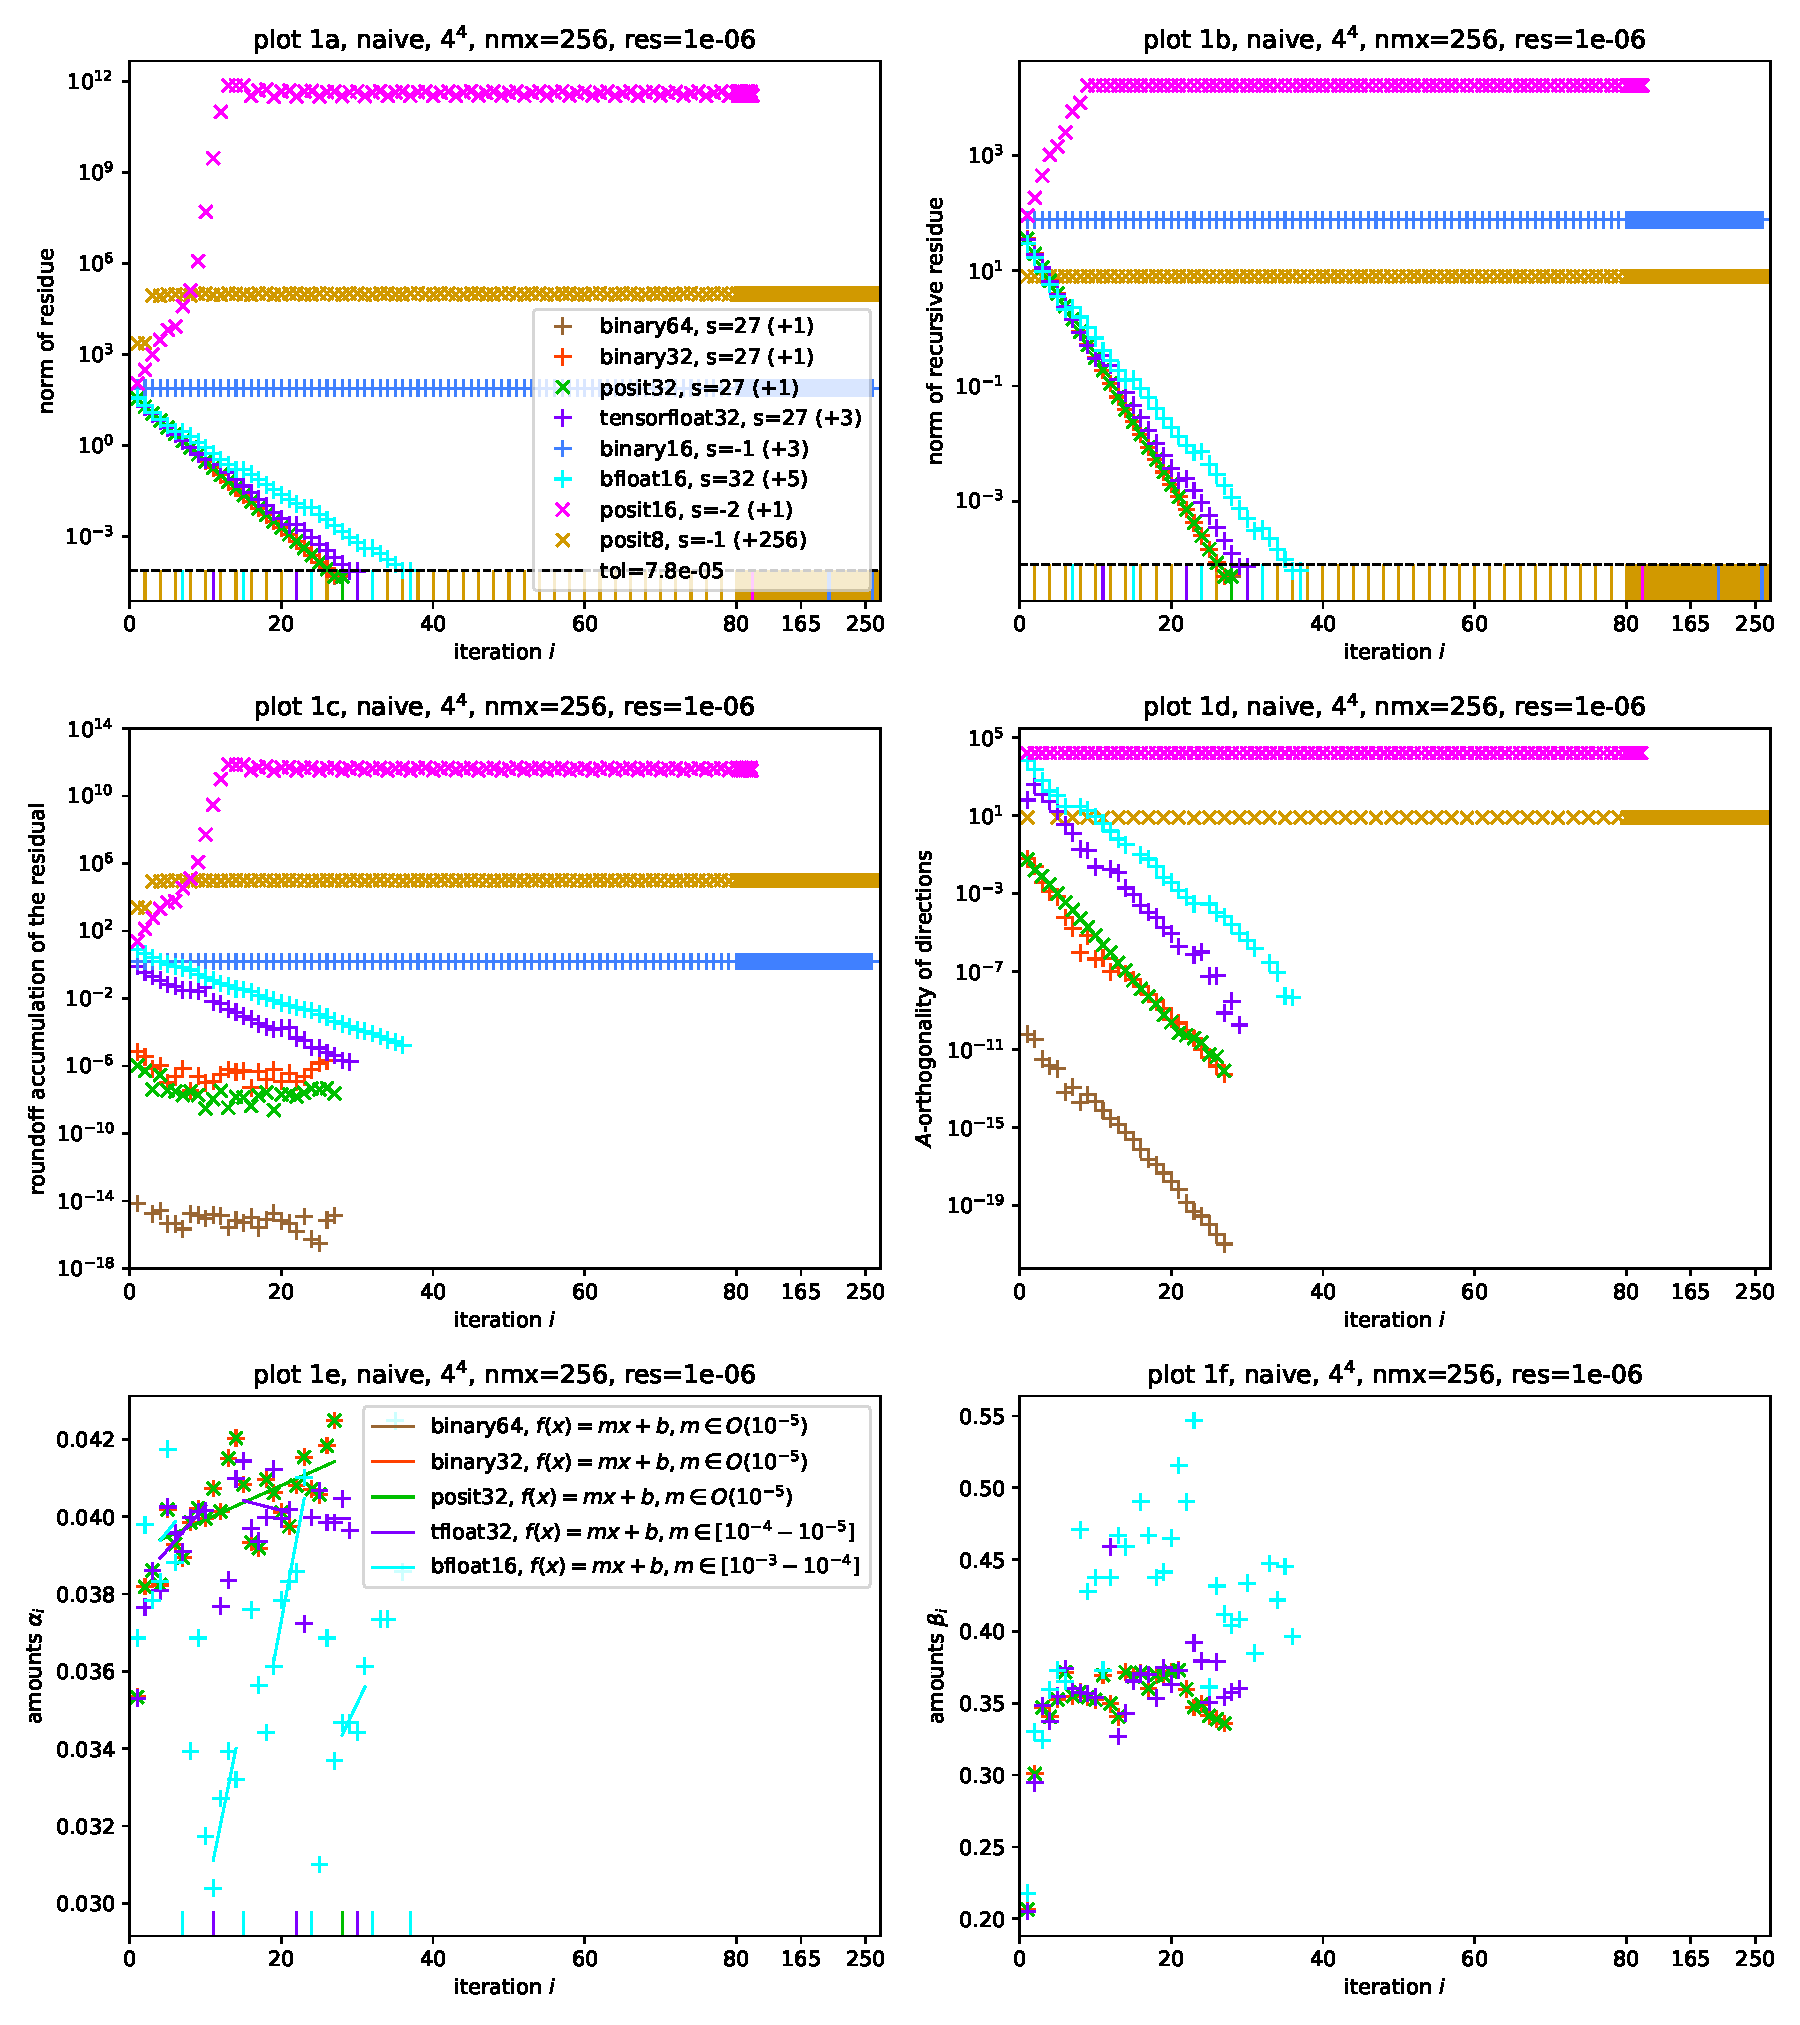
\includegraphics[width=1.0\linewidth]{plots/cgne_final_0}}
    %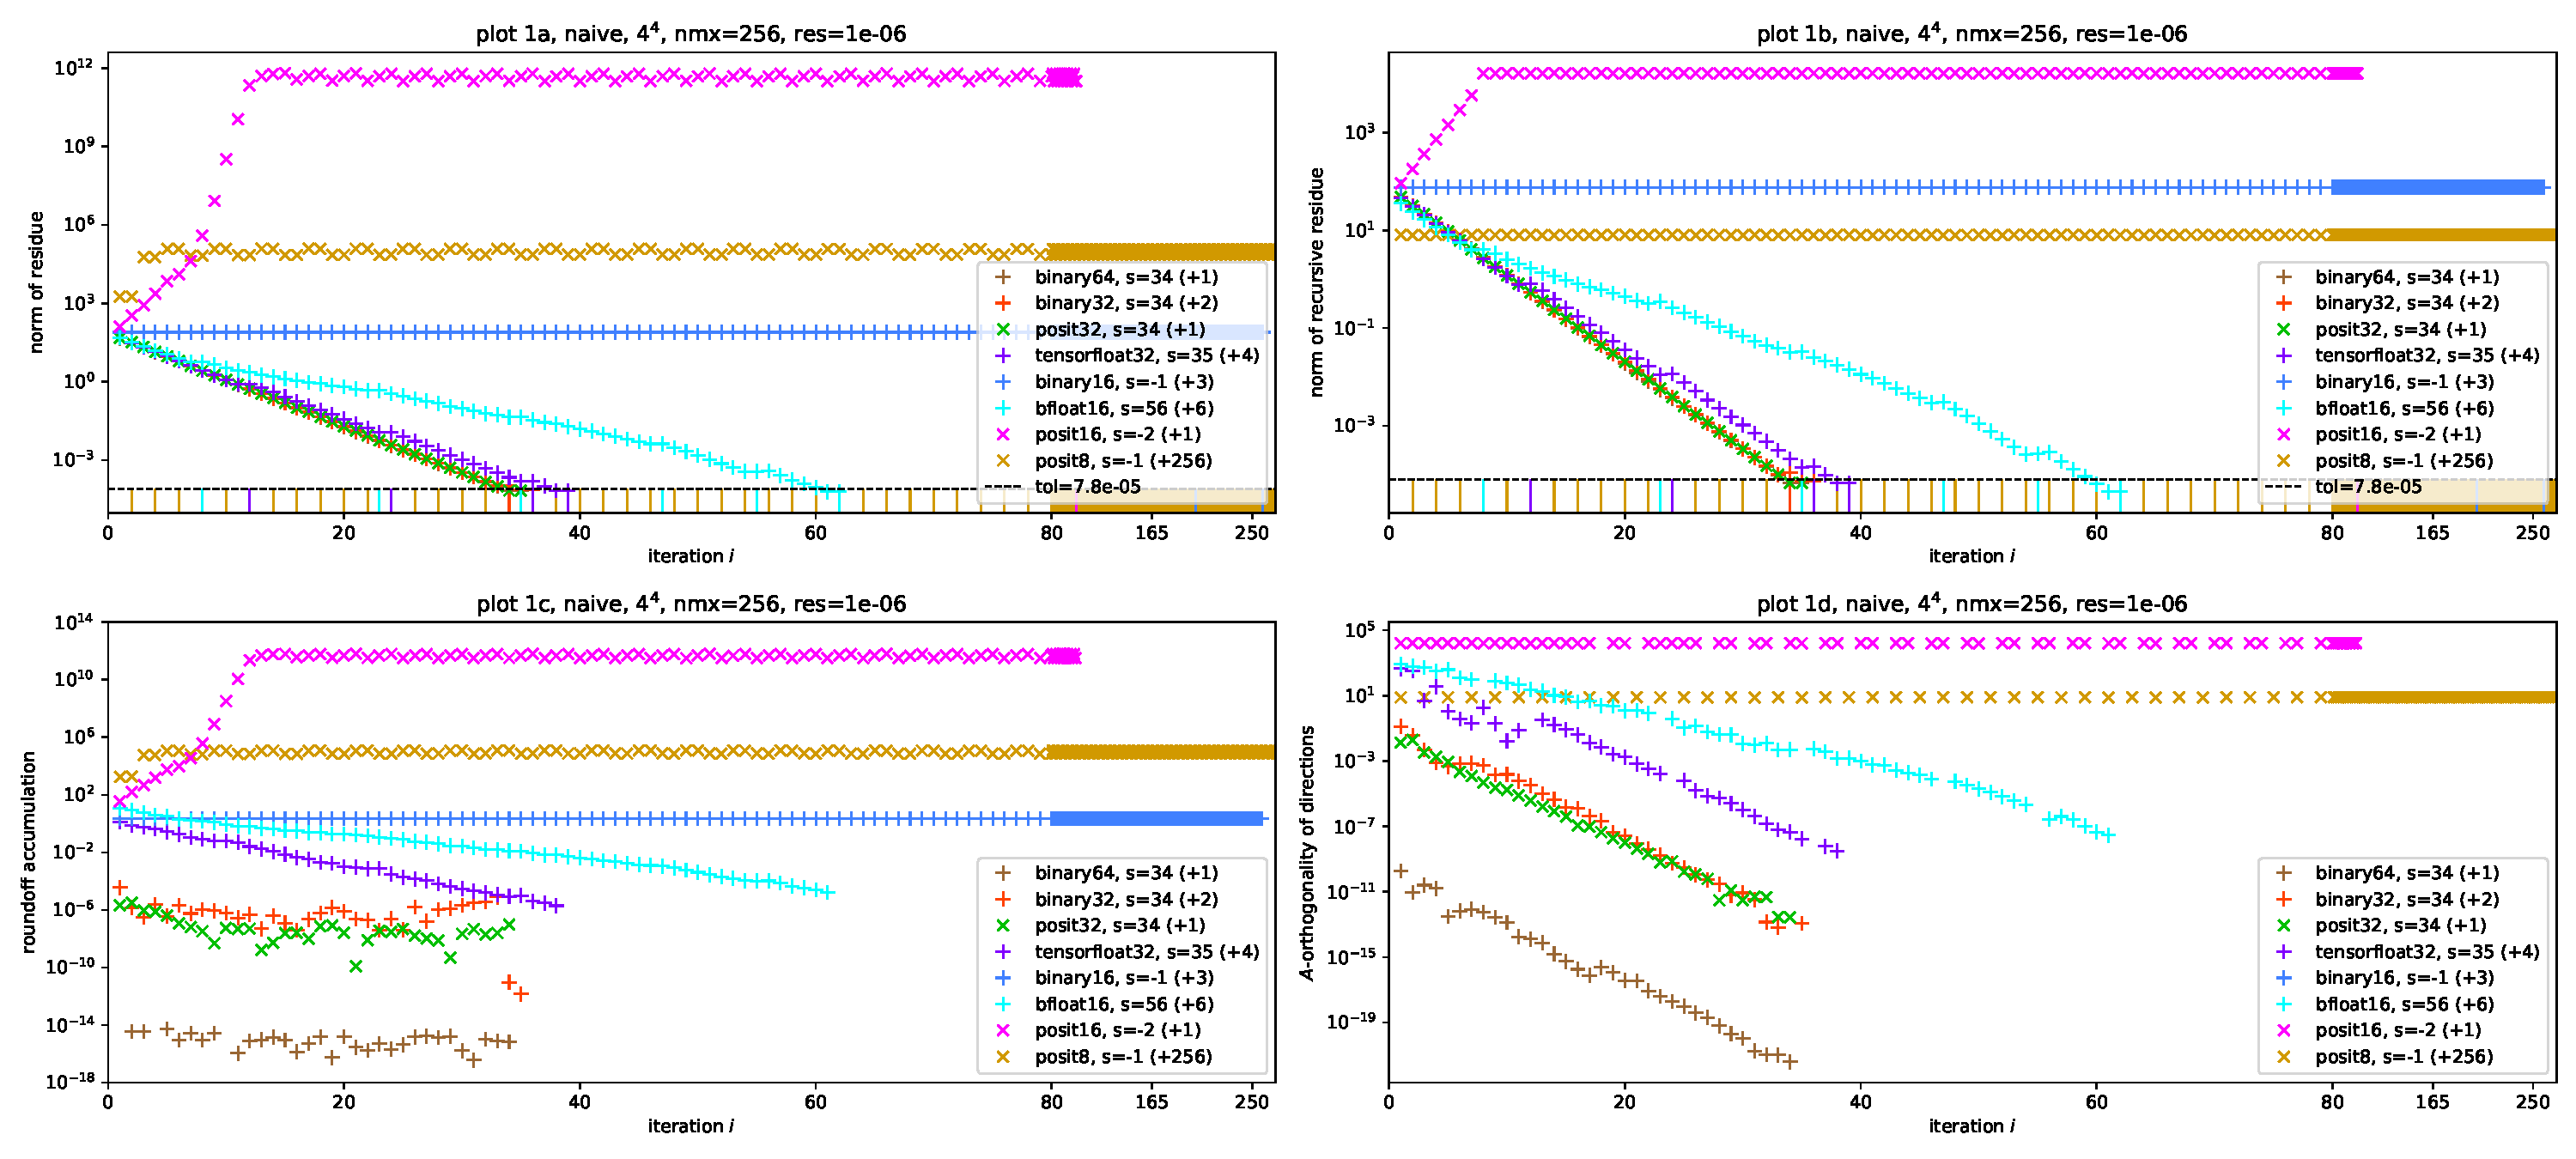
\includegraphics[width=1.0\textwidth]{plots/cgne0}
    \caption{Convergence analysis of a conjugate gradient run, where \gls{binary32} was replaced by one of the simulated datatypes. The number \code{s} describes the number of normal steps needed (the value of \code{status}), whereas the numbers in the brackets indicate the number of reset steps. All reset steps are indicated by ticks at the dashed black line denoting the tolerance limit. The iterations will always go up to \code{nmx=256}, but the range \num{80}-\num{256} is compressed since the most interesting behaviour happens before step \num{80} for most of the simulated datatypes. The 6 plots show the naive replacement of the \gls{binary32} datatype with the simulated one. This means that every single variable containing a \gls{binary32} was replaced with a variable of the simulated datatype. Plot \textit{1a} shows the exact residue \eqref{eq:residual_exact} calculated in every iteration using the Dirac matrix and the source vector both in \gls{binary64}, whereas plot \textit{1b} shows the norm of the recursively calculated residue \eqref{eq:residual_recursive} (cast from the simulated datatype to \gls{binary64}). The relative residue suffers round-off accumulation because of the recursive calculation; this is the difference between plots \textit{1a} and \textit{1b}, which is plotted in plot \textit{1c}. Plot \textit{1d} shows the $A$-orthogonality of the current direction to the last direction, namely the value of $\vec{p}_{i}^\dagger A \vec{p}_{i+1}$. The last 2 plots, \textit{1e} and \textit{1f}, show the values of the amounts $\alpha_i$ and $\beta_i$ (see equations \eqref{eq:alphai} and \eqref{eq:betai}) in every iteration, but only of the datatypes that converged (\code{status>0}). The lines in plot \textit{1e} are linearly fitted to the data points ($f(x) = m x + b$). The number range of the slope $m$ is given in the plot legend.}
    \label{fig:cgne:naive}
\end{figure}

\begin{figure}
    \centering
    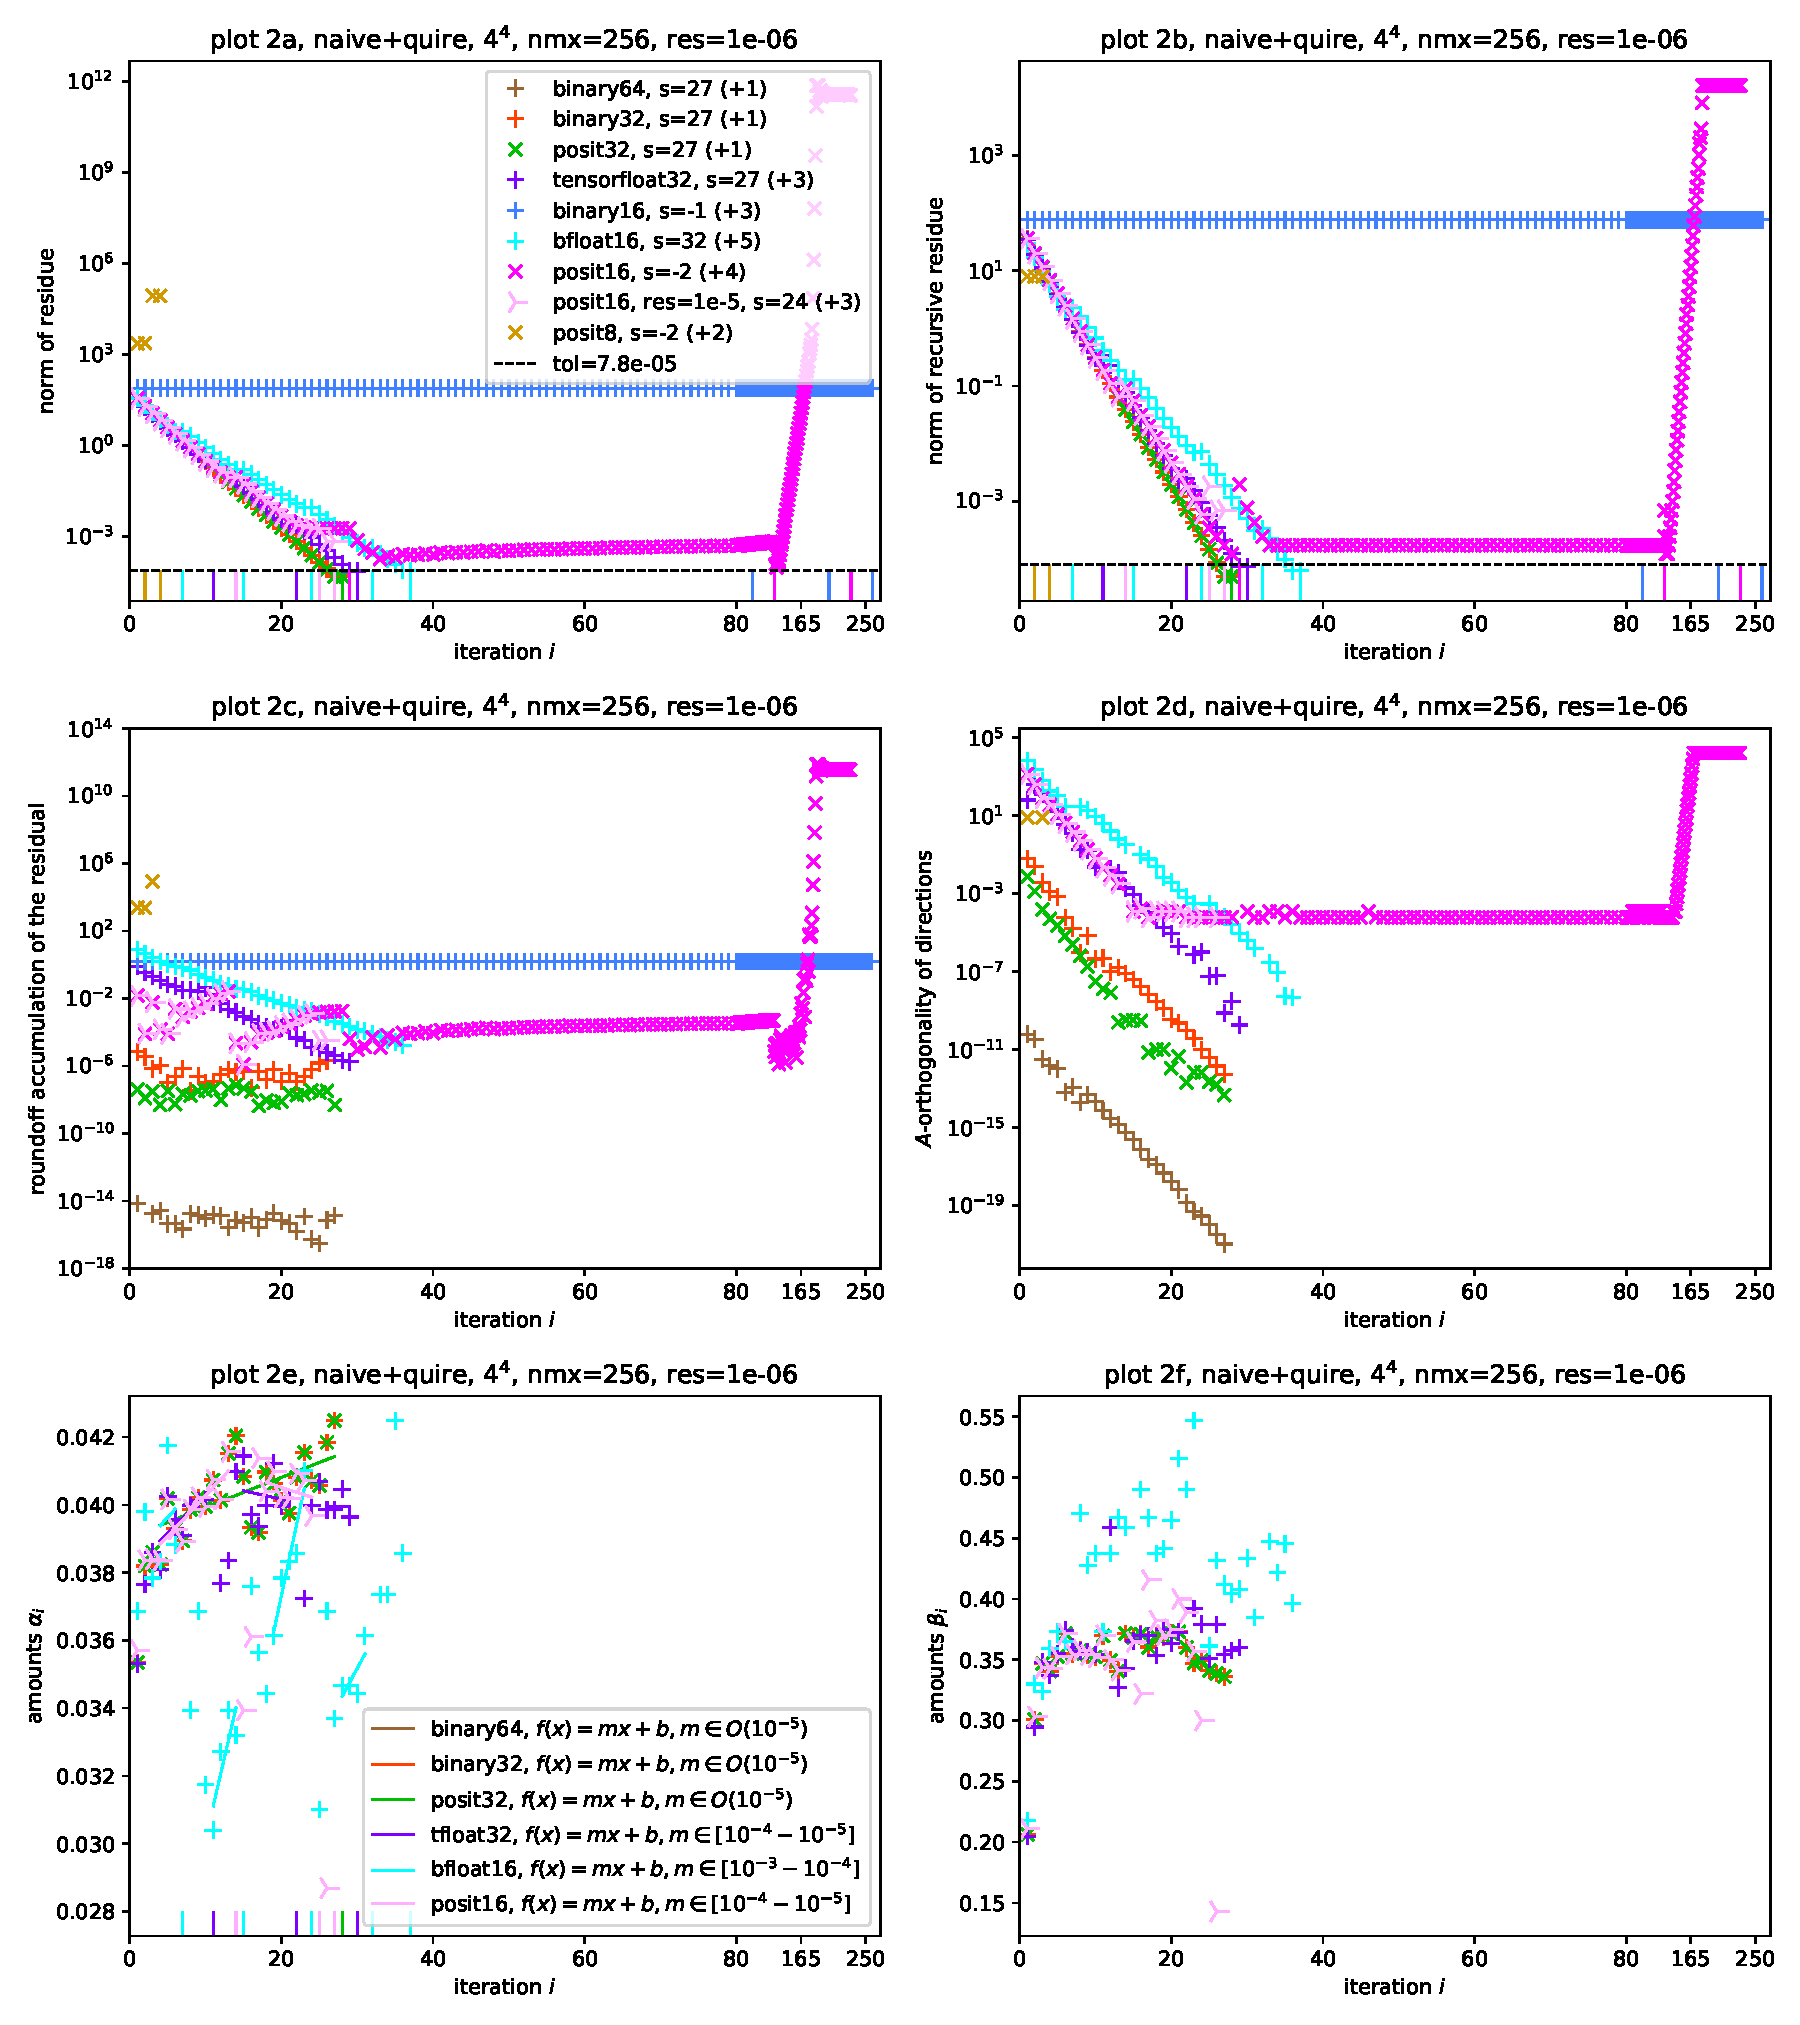
\includegraphics[width=1.0\textwidth]{plots/cgne_final_1}
    \caption{In these plots, the posits were utilising \glspl{quire} as their collective variables, the remaining setup was the same as for figure \ref{fig:cgne:naive}, therefore the floating point datatypes show exactly the same values, only posits changed their behaviour.}
    \label{fig:cgne:quire}
\end{figure}

\begin{figure}
    \centering
    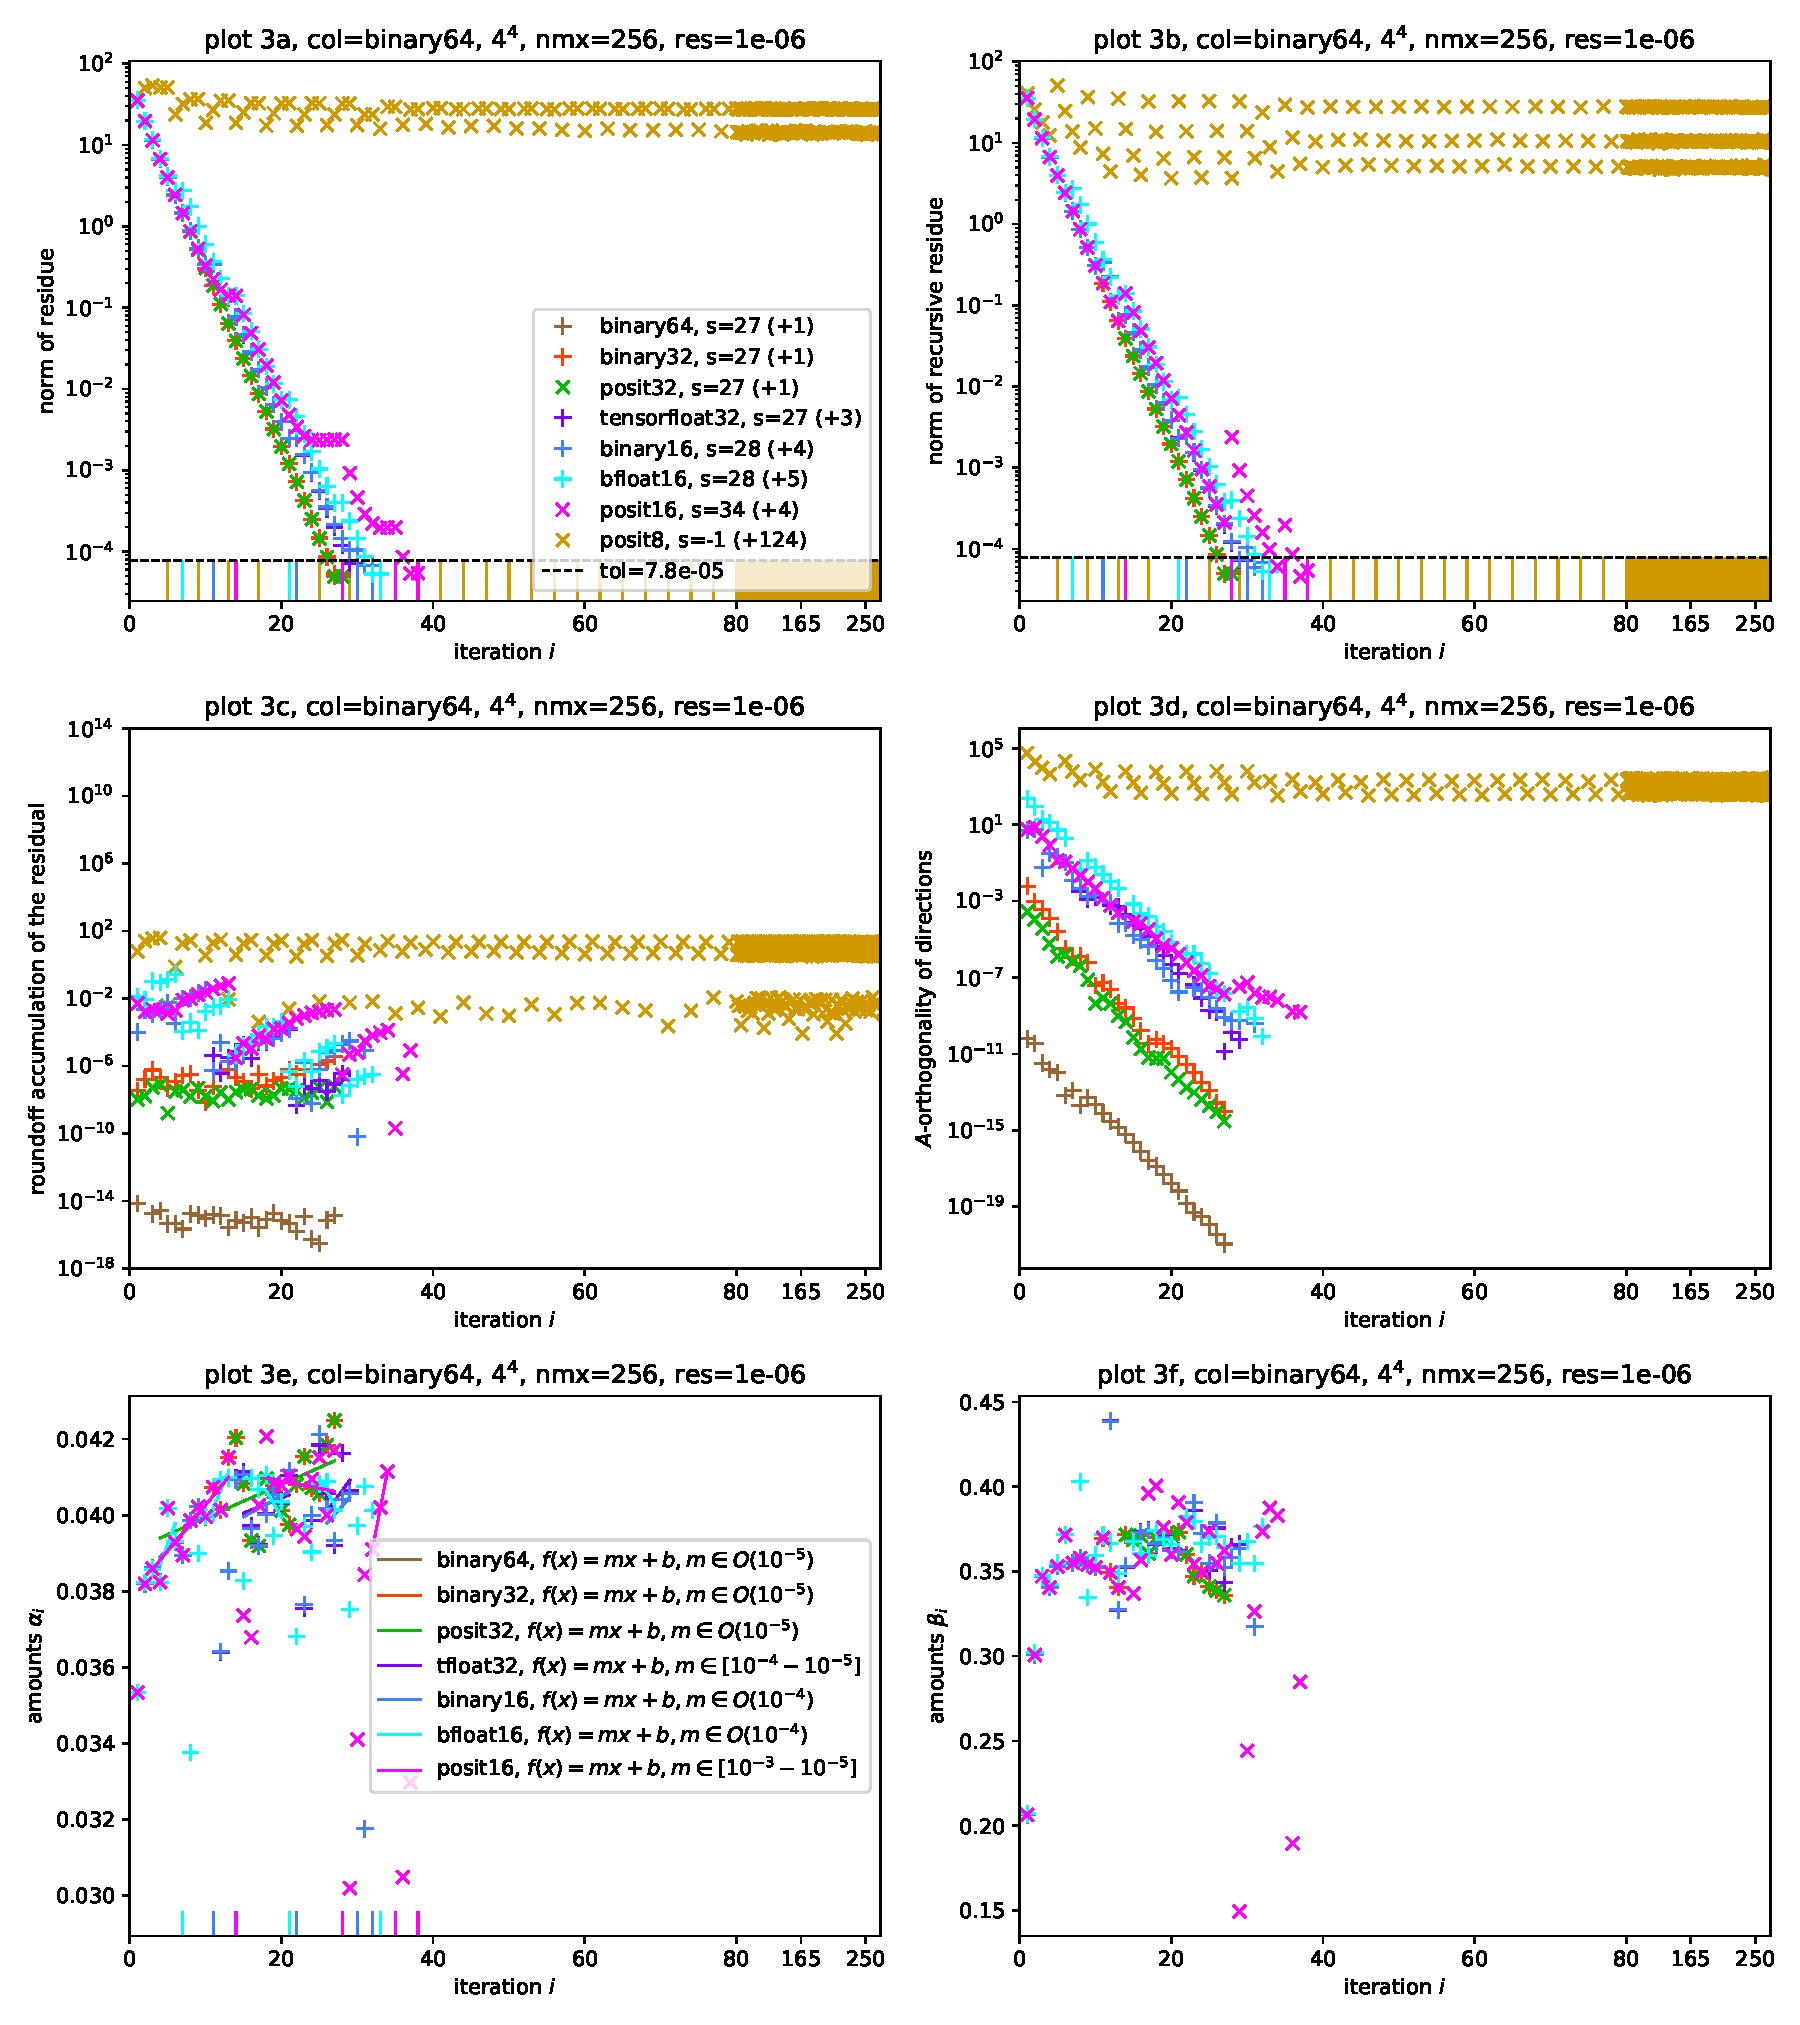
\includegraphics[width=1.0\textwidth]{plots/cgne_final_2}
    \caption{The 6 plots introduce a slightly smarter replacement. All collective variables such as norms where calculated in \gls{binary64}, such that a datatype with a small number range such as \gls{binary16} may not over- or underflow when calculating the norm of a vector full of said datatype. This replacement resembles the \gls{quire} for posits. Using this replacement, even heavily reduced datatypes like \gls{binary16} and \gls{posit16} converged and threw a result of equal quality as the one simulated with \gls{binary64}.}
    \label{fig:cgne:col64}
\end{figure}


\begin{figure}
    \centering
    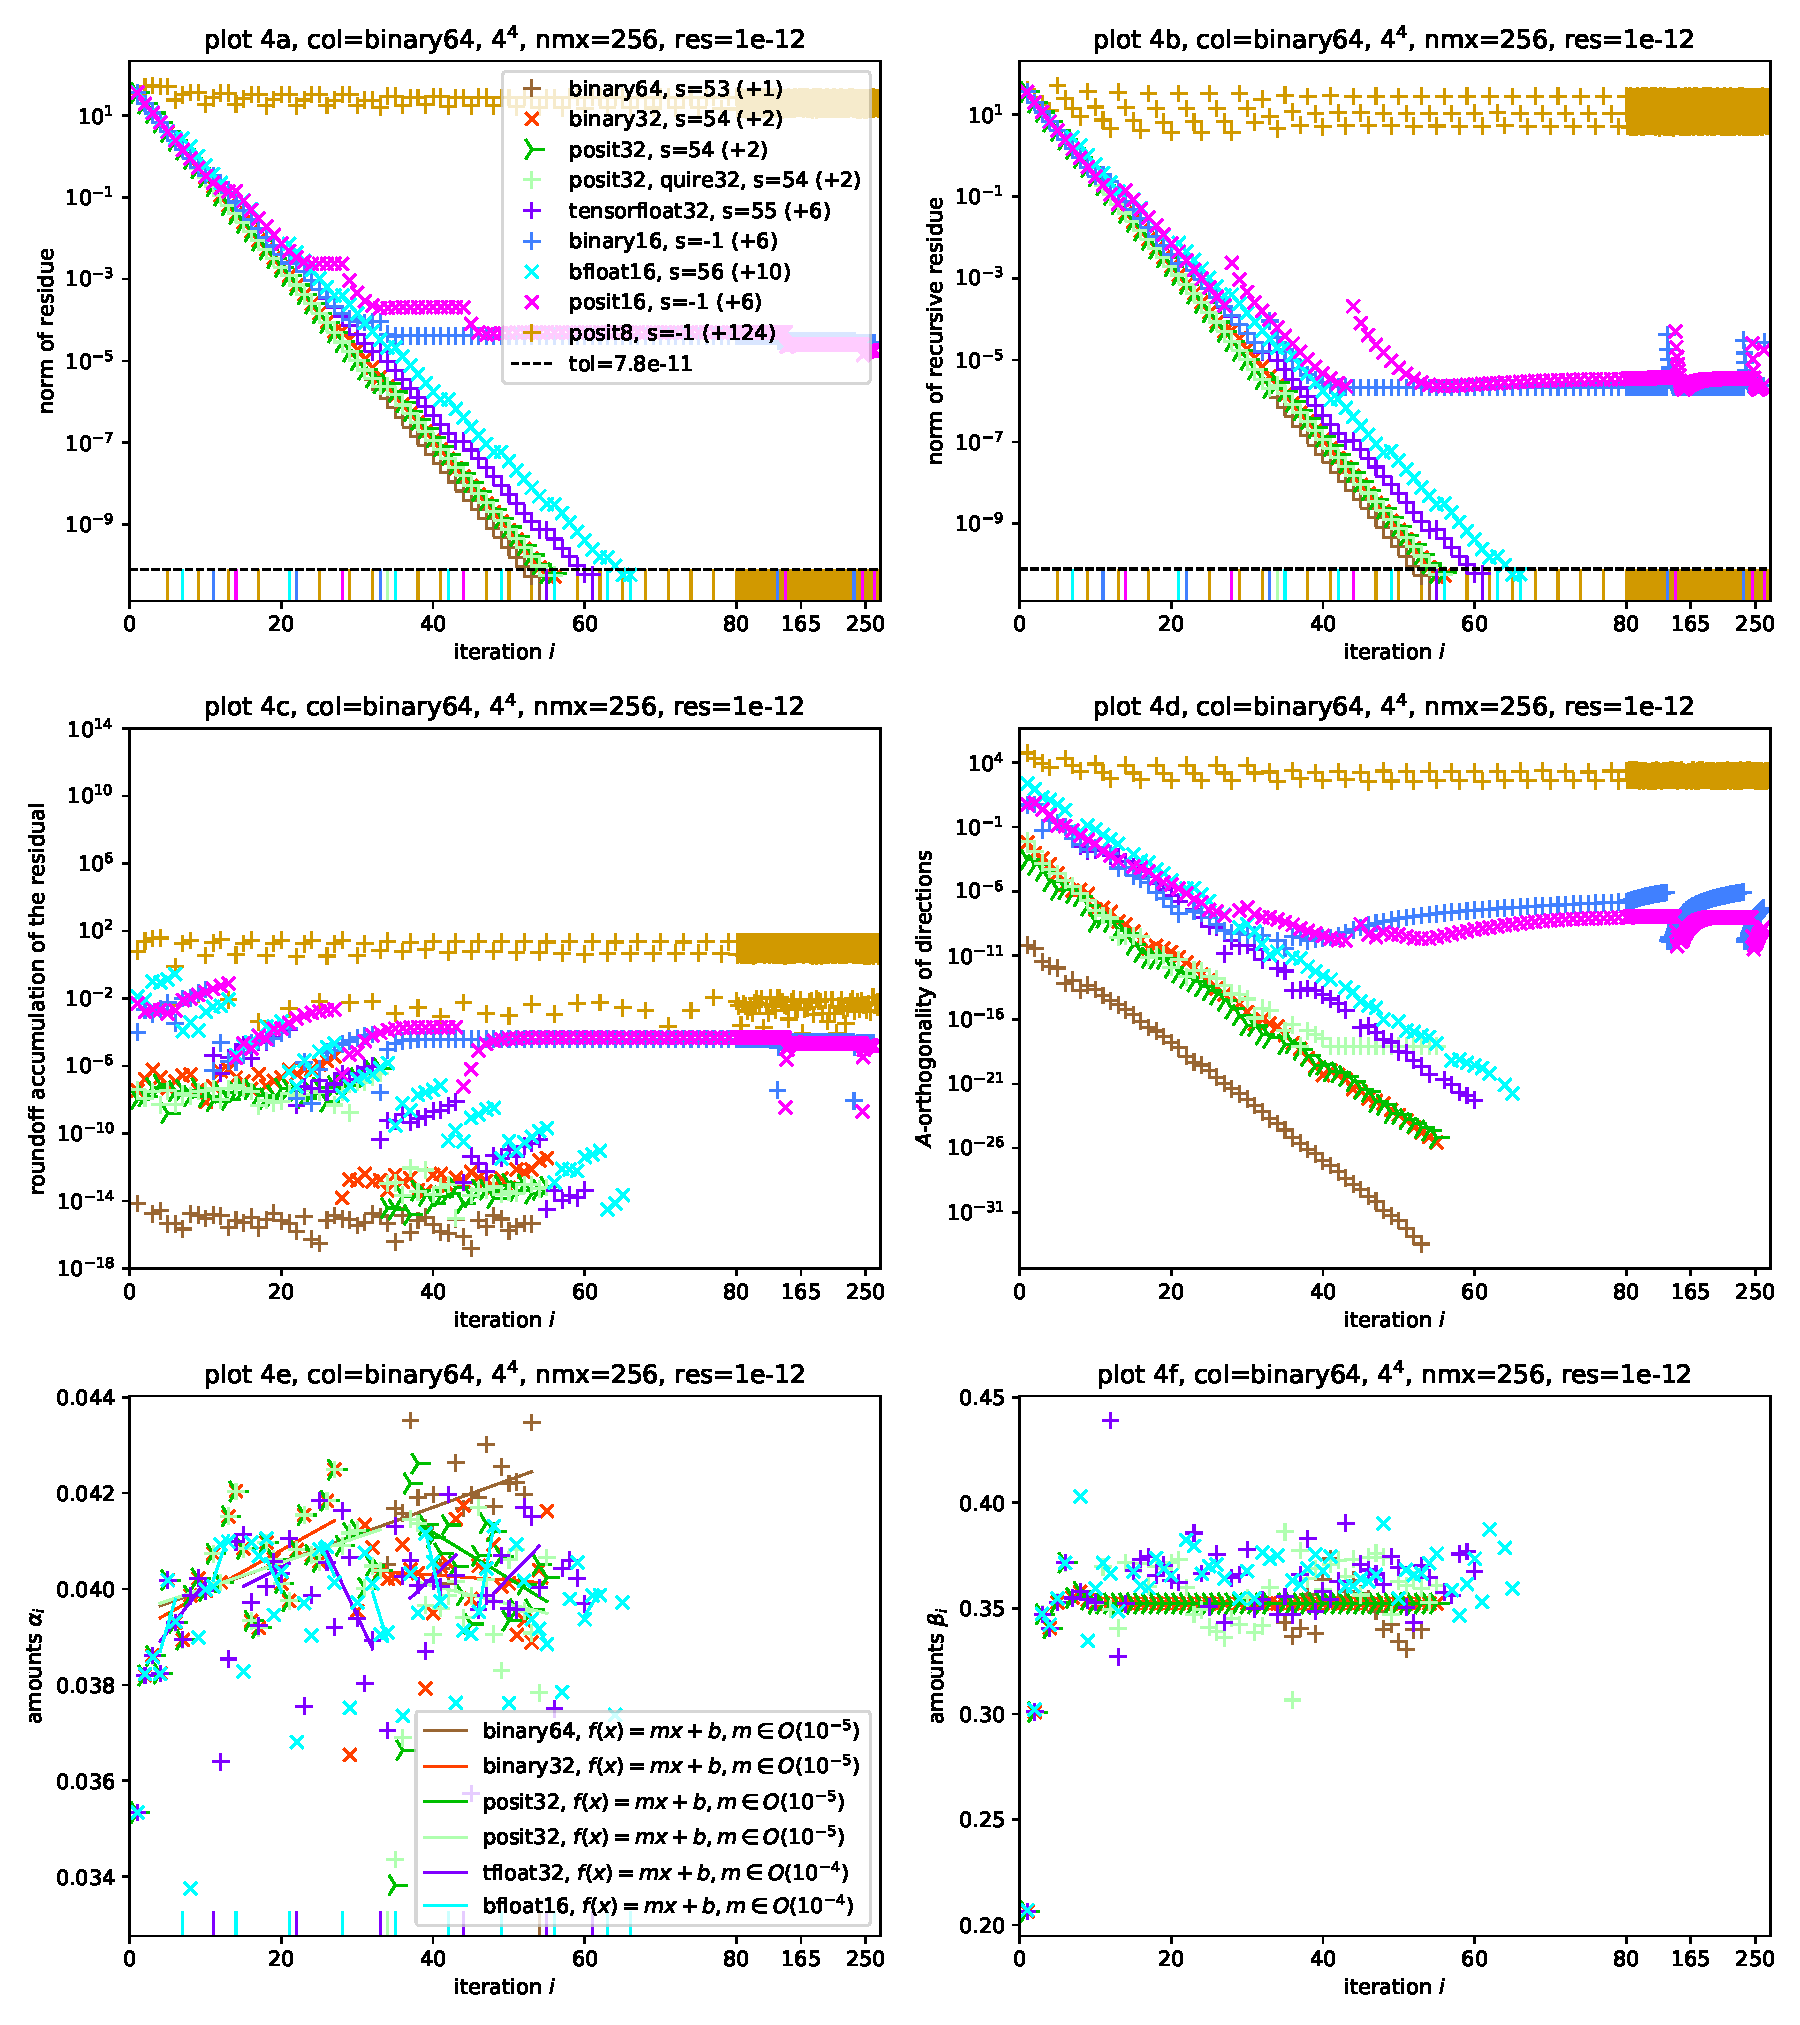
\includegraphics[width=1.0\textwidth]{plots/cgne_final_3}
    \caption{The configuration in this series of plots is equal to Figure \ref{fig:cgne:col64}, besides the value of \code{res} - the desired relative residue of the calculated solution - is set to $10^{-12}$ instead of $10^{-6}$. Notice that $10^{-12}$ is outside the representable number range of the datatypes that did not converge; \gls{binary16}, \gls{posit16} and \gls{posit8}.}
    \label{fig:cgne:res12}
\end{figure}

\subsubsection{Discussion of figures \ref{fig:cgne:naive} - \ref{fig:cgne:res12}}

Figures \ref{fig:cgne:naive}, \ref{fig:cgne:quire}, \ref{fig:cgne:col64} and \ref{fig:cgne:res12} contain all relevant data. It is expected in general that the plots show datatypes of the same bit-length in clusters and exhibit a hierarchy in precision and exponent range; more precision and larger exponent range should end up in faster convergence. Thus we expect the following hierarchy (where smaller means convergence in fewer steps)

\begin{align}
    \textcolor{cbrown}{\text{binary64}} < \textcolor{cgreen}{\text{posit32}} \leq \textcolor{cred}{\text{binary32}} \leq \textcolor{cpurple}{\text{tensorfloat32}} \leq \textcolor{cturquois}{\text{(1)}} \leq \textcolor{cpink}{\text{posit16}} \leq \textcolor{cblue}{\text{binary16}} \leq \textcolor{cturquois}{\text{(2)}} < \textcolor{cyellow}{\text{posit8}}, \label{eq:hierarchy}
\end{align}

where \textcolor{cturquois}{\text{bfloat16}} could be either at position \textcolor{cturquois}{\text{(1)}} or \textcolor{cturquois}{\text{(2)}}, depending on what is more important; precision or number range.

In Figure \ref{fig:cgne:naive} where the datatype is naively replaced by the simulated datatype, it can be concluded that only datatypes with large enough number ranges converged. \gls{binary64}, \gls{binary32} and \gls{posit32} converged each after \code{status=27} steps with one reset step. The less precise \gls{tensorfloat32} took \code{status=27} ($+3$) and the even less precise \gls{bfloat16} needed \code{status=32} ($+5$) steps. Such a hierarchical result was expected since they have the same exponent range and thus approximately the same number range, but differ only in precision (see Table \ref{tab:formats}). Notice that the less precise the datatype, the more reset steps are needed. This happens because the precision limit of the simulated datatype is reached faster, if the datatype has less precision.

The round-off accumulation error of \gls{posit32} is slightly better than the one of \gls{binary32}, although defeated by $8$ orders of magnitude of \gls{binary64} because of its much more precision. It is notable to remark that the round-off accumulation does not increase substantially from step to step, what would be expected from a recursive calculation. The reason for the small difference between \gls{binary32} and \gls{posit32} could be that the involved real numbers are closer to representable numbers in \gls{posit32} than in \gls{binary32}. Posits have a larger number density around \num{1} compared to floats of the same bit-length, and therefore more precision in that regime (see Figure \ref{fig:number_line} for the example of \gls{binary16} versus \gls{posit16}). Posits also have more numbers, because they have no \acrshortpl{nan}. Round-off accumulation is specially dependent on the precision of the datatype, which makes sense; the lower the precision, the higher the round-off accumulation. The difference in $A$-orthogonality is negligible for \gls{posit32} compared to \gls{binary32}, but again clearly surpassed by \gls{binary64}.

\gls{binary16} did not converge (\code{status=-1}) after the maximal number of \code{nmx=256} steps. Its footprint is absent in plot \textit{1d}, because it consisted only of \acrshortpl{nan} and infinities, causing $\alpha_i = 0$ and $\beta_i = 1$. This implied that $\vec{r}_i = \vec{r}_{i+1}$ and $\vec{p}_{i+1} = \vec{r}_{i+1}$ and therefore $\vec{x}_{i+1} = \vec{x}_{i}$ and the algorithm stalled. This explains the residues not changing in plots \textit{1a} and \textit{1b}. The reason for the first infinity was an overflow when calculating the norm of $\vec{b}$ in the very first iteration. This suggests that the limited number range of \gls{binary16} might not be enough (at least for a naive replacement), comparing to \gls{bfloat16} with the same bit-length, but larger number range that was able to converge, although very slowly.

The behaviour of \gls{posit8} is very similar to \gls{binary16}, but without the overflow, because posit do not overflow by definition. Instead the biggest representable number is returned or in case of an underflow the smallest representable number is returned \cite{posit2018standard}. The algorithm stalled at a value of the norm of the recursive residual of $\norm{\vec{r}_i} = 8$. The biggest \num{8}-bit posit number with exponent bits $es=0$ is $2^6 = 64$, so the norm squared cannot be bigger than $64$ and the norm itself cannot be bigger than $8 = \sqrt{64}$ (see plot \textit{1b}). This happened in the first step, whereas the actual residual in \gls{binary64} was $\backsim 10^3$. The amounts $|\alpha_i| \ll 1$ in iterative steps are therefore very small causing $\vec{x}_{i+1} \approx \vec{x}_i$. Significant changes in $\vec{x}_i$ will not happen and convergence is unlikely. Also notice that \gls{posit8} had \num{256} reset steps, which means that after every step there was a reset step. The steps where caused by the very high precision limit of \gls{posit8}. The value of \code{PRECISION\_LIMIT} is $100*\code{MACHINE\_EPSILON}$, which has a value of \num{3.125} for \gls{posit8}.

The story of \gls{posit16} is very similar, just that the maximal representable value with $es=1$ is \num{268435456} and the square root of this is \num{16384} which is reached after $8$ steps (see plot \textit{1b}). The actual residual in the $8$-th step was $\backsim 10^7$, the algorithm diverged and then stalled. Iterative steps are therefore mostly too small and convergence is unlikely.

We observe that number range is more important than precision, when naively replacing the datatype, but the higher the precision, the faster the convergence and the less reset steps needed.

In Figure \ref{fig:cgne:quire} the replacement utilised the possibility to use \glspl{quire} for the posit runs. Therefore, the numbers for the float datatypes are exactly equal to the ones in Figure \ref{fig:cgne:naive}, because floats have no such feature. They are not discussed again.

Comparing plots \textit{1c} and \textit{2c} and looking at \gls{posit32}, one can see that the round-off accumulation in the residual due to its recursive calculation is slightly better than without using the \gls{quire}. This makes sense, because \glspl{quire} introduce deferred rounding. This is exploited specially in the calculation of norms and matrix-vector products. It also results in a somewhat better maintaining of $A$-orthogonality for the direction vectors.

However, the data points of \gls{posit16} bear little resemblance to its previous or later runs. It comes much closer to the target residual tolerance than in the last simulation, but it is still not reached. The tolerance is within the number range of \gls{posit16}, even so it did not converge. The reason for this is that the smallest representable number in \gls{posit16} is $2^{-28}$. The \gls{quire} for \gls{posit16} has the same number range, despite the \num{128} bits in length. Every norm squared of a non-zero vector must be larger to equal to this number, because posit do not underflow. Therefore the norm is always larger or equal to $\sqrt{2^{-28}} = 2^{-14} \approx 6.1 \cdot 10^{-5}$. The tolerance of $7.8 \cdot 10^{-5}$ - even though larger than that number - is perhaps still too close. Comparing the \textcolor{clightpink}{lightpink} values, that are \gls{posit16} as well, but the relative residual \code{res} is set to $10^{-5}$ instead (the tolerance being one order of magnitude larger), they converged after only \code{status=24} steps. This suggests that the reason for the strange behaviour lies in the relative residual that was chosen too close to the lowest number above zero of the number regime.

Using the same arguments and analysis, \gls{posit8} had no chance to give a meaningful result.

In Figure \ref{fig:cgne:col64}, a smarter replacement was done. All variables that have a collective role suffer from overflow. For example the norm of a vector $\vec{v} \in \mathbb{R}^n$ is 

\begin{align*}
    \norm{\vec{v}} = \sqrt{ \sum_{i=1}^{n} v_i^2 }.
\end{align*}

The number below the square root may be much bigger before squaring than after. If we calculate the norm in \gls{posit8}, the result will be $\norm{\vec{y}} \leq 8$. More importantly, when using a datatype that overflows such as \gls{binary16}, the value after squaring might be perfectly fine, but the value under the square root could be outside the range of representable numbers, $\sqrt{\infty} = \infty$ and $\sqrt{0} = 0$. This is cured if the collective variable is of a datatype with larger number range than the underlying datatype that is summed over. In Figure \ref{fig:cgne:col64} all collective variables were of type \gls{binary64}.

The data of \gls{binary64} exhibits no significant alterations. Again comparing \gls{binary32} and \gls{posit32} with their previous data points, we see that the round-off accumulation of \gls{binary32} is a little better and \gls{posit32} is approximately the same as with the \gls{quire}, suggesting that when using posits utilising the \gls{quire} is probably sufficient.

Looking at \gls{tensorfloat32}, it has the same exponent range as \gls{binary32}, but less precision and it has the same number of mantissa bits as \gls{binary16}, but at a higher exponent range. Compared to \gls{binary16}, both datatypes have the same amount of numbers to be distributed in their respective number range. It is expected to perform worse or equal to \gls{binary32}, but better or equal to \gls{binary16} and \gls{bfloat16}. Therefore it's expected to converge in $27 \le \code{status} \le 28$ steps, see equation \eqref{eq:hierarchy}. This is indeed the case with \code{status=27} steps. We see that the larger number range compared to \gls{binary16} has little to do with speed of convergence. This is because the number regime is within the \gls{binary16} regime, except for collective variables. This explains as well why \gls{tensorfloat32} performed precisely as in the naive replacement, Figure \ref{fig:cgne:naive}, but the round-off accumulation is better because of the more precise collective variables.

The \gls{bfloat16} with even less precision but comparable number range of \gls{tensorfloat32} converged in \code{status=28} steps as well, but needed two more reset steps, tightening the previous conclusion about speed of convergence.

The most interesting data points are the ones of \gls{binary16} and \gls{posit16} that both were able to converge in \code{status=28} and \code{status=34} steps respectively. They performed quite similar, even though it would be expected that \gls{posit16} would perform a slightly better because of the bigger number range and bigger number density in relevant number regimes (see Figure \ref{fig:number_line}). In plot \textit{3c} the increase of round-off accumulation can be observed for \gls{binary16} and \gls{posit16} in steps where the real residue changes (where the algorithm makes progress, see for example: steps \num{1} to \num{10}). Notice that, when the real residue stalls and the recursive residue still (wrongly) decreases, the round-off accumulation will saturate until the order of magnitude of the two numbers becomes too large such that their difference is dominated by the larger number. This can the seen in the data points of \gls{posit16} in plot \textit{3a}. It suggests that the precision limit was chosen too low for the datatype. Notice that the precision limit is defined to be \num{100} times the \code{MACHINE\_EPSILON} of the datatype. The \code{MACHINE\_EPSILON} for the posit datatypes is quite misleading, because it gives us (by definition) the precision of numbers around \num{1}. This is the regime where posits are most precise, their precision falling off very rapidly when leaving it. Thus for \gls{posit16} in the regime $10^{-1}$ the \code{MACHINE\_EPSILON} is correct (seen at iteration \num{14}), whereas in the regime $10^{-3}$ it is chosen to small and we can see a staircase-shape around the reset steps at iterations \num{28} and \num{35}. Such a stalling of the real residue should be avoided at any cost, because the algorithm stalls as well in that case. The \code{MACHINE\_EPSILON} is defined to be the difference between \num{1} and the lowest number above \num{1}. For floats this definition makes more sense, because their precision does not fall off that fast, but for posits which are most precise around \num{1} this gives a too precise value, not reflecting the real precision of posits in their whole number range correctly. Instead, the machine epsilon should be a function of the number regime, increasing when going far away from \num{1}. This is the reason for the staircase-shaped curve of \gls{posit16} in plot \textit{3a}. The phenomenon is even more prominent for \gls{posit16} in plot \textit{4a} of Figure \ref{fig:cgne:res12}. The \gls{posit32} does not have this problem, because its \code{MACHINE\_EPSILON} is sufficient for the number regime used in the algorithm. When demanding lower relative residuals, staircase-shapes should be expected for \gls{posit32} as well.

Comparing \gls{binary16} with \gls{bfloat16} and \gls{tensorfloat32}, we see again that exponent range is less relevant than precision. Precision determines the amount of reset steps.

Figure \ref{fig:cgne:res12} shows all the simulated datatypes using a collective datatype of \gls{binary64} just as in Figure \ref{fig:cgne:col64}, but with a relative residual of $10^{-12}$ instead. This might be a more realistic scenario. The last row resembles the predicted hierarchy \eqref{eq:hierarchy} particularly well. Notice that $10^{-12}$ is outside the representable number range of \gls{binary16}, \gls{posit16} and \gls{posit8}. This means that these datatypes have no chance to reach the target tolerance, therefore we expected them not to converge. This is indeed the case. We also see that \gls{binary16} and \gls{posit16} both are not able to go below $10^{-5}$, meaning the tolerance in the third row was chosen very close to the minimum possible, but still converging tolerance (see also discussion of \gls{posit16} in Figure \ref{fig:cgne:quire}). Both datatypes make no further significant progress after step \num{45}. It can also be seen that even the recursive residue stalls or increases - an indicator that the datatype has reached its limits.

The comparison between \gls{binary32} and \gls{posit32} is again of insight. Their difference is subtle. We see that both needed the same amount of steps. Round-off accumulation and $A$-orthogonality are again slightly better, making \gls{posit32} the overall better \num{32}-bit datatype for the problem. The reason for this goes down to the higher precision of posits in the relevant number regime. Looking at the \textcolor{clightgreen}{lightgreen} values, that are \gls{posit32} as well, but utilising the \gls{quire} instead of \gls{binary64} as collective variable, we observe the same amount of steps to convergence, but round-off accumulation is slightly worse. It might be an unfair comparison, because \gls{binary64} as collective variable has more precision, surpassing even the deferred rounding employed by the \num{512}-bit \gls{quire} for \gls{posit32}. In plot \textit{4d} the \gls{posit32} with \gls{quire} will not go below some fixed value. The reason for this is the lowest \gls{posit32} value with exponent bits \code{es=2} is $8^{-30}$ and the norm of a \gls{posit32}-vector with at least one non-zero component must be bigger or equal to the square root of this; $1.15 \cdot 10^{-18}$. This suggests that when choosing \code{res} to be smaller than $10^{-18}$, we expect \gls{posit32} not to converge anymore in analogy to \gls{posit16} in the second row.

Since \gls{binary16} was able to converge in Figure \ref{fig:cgne:col64}, this suggests that the number regime is within \gls{binary16} giving \gls{posit32} more precision in that regime over \gls{binary32}

Finally, compare the \num{3} datatypes with the same exponent range, but different precisions; \gls{binary32}, \gls{tensorfloat32} and \gls{bfloat16}. The less precision, the slower the convergence. The price to go from \num{23} to \num{10} mantissa bits results in \num{1} more conjugate gradient step as well as \num{4} more reset steps. When going further down to \num{7} mantissa bits again \num{1} more regular step and \num{4} more reset steps where needed to finally bring \gls{bfloat16} to convergence after \code{status=56} regular conjugate gradient plus \num{10} reset steps. Bearing in mind that it uses only \num{16} bits, this is a remarkable result. It performed way better than its \num{16}-bit competitors.

We also see in plot \textit{4a} that all datatypes start to converge by the same speed (all slopes are equal). The actual residual of the datatype with the lowest precision, namely \gls{bfloat16} with \num{7} mantissa bits, resets first, followed by \gls{binary16} and \gls{tensorfloat32} which have both \num{10} mantissa bits. The next one is \gls{posit16}, because it has more precision than \gls{binary16} in the relevant regime, followed by \gls{binary32} with \num{23} mantissa bits and later by \gls{posit32}, where the same argument as before holds. The curve of \gls{binary64} would also reset at some point, but that is outside the scale.

Specially plot \textit{4a} suggests that we can start to calculate in a datatype with \num{16} bits of length until we fall below a constant, to be determined value (that depends on the datatype), then continuing the calculation in a datatype with \num{32} bit-length until that number regime is exhausted as well, again switching to a \num{64} bit datatype to finish the calculation.

\subsubsection{$8^4$ lattice}

In order to make sure that the previous analysis is consistent and the physics involved were relevant, the same data was extracted from a $8^4$ lattice and some of the plots were remade from the new data, see Figure \ref{fig:cgne8}. Only the datatypes \gls{binary64}, \gls{binary32} and \gls{binary16} were simulated. In principle, the data tells the same story. The main difference to figures \ref{fig:cgne:col64} and \ref{fig:cgne:res12} is that more steps were needed to converge, because the Dirac matrix is much larger than before, although only \num{0.04}\% of all components were non-zero, compared to \num{2}\% in the $4^4$ lattice of the previous analysis. In plots \textit{2a} to \textit{2f}, were the relative residue was chosen to be $10^{-12}$, we again see the saturation of \gls{binary16} marking the lower limit of the datatype. After every reset step, a jump in round-off accumulation can be seen, because the residual in the reset step is calculated in higher precision. It is interesting that the round-off accumulation in the final steps of \gls{binary16} come very close to those of \gls{binary32} (see plot \textit{1c}). A reason for this could be the clustering of reset steps just before convergence, giving very accurate results with little round-off, even for less precise datatype. We also see that the speed of convergence does not significantly depend on the precision of the datatype, only the amount of reset step does, thus the less steep slope of \gls{binary16}. When the lower limit of the datatype is reached, the slope becomes zero and the residual shows no striking reduction anymore. This is were the datatype should be switched to one with a larger number range.

\begin{figure}[h]
    \centering
    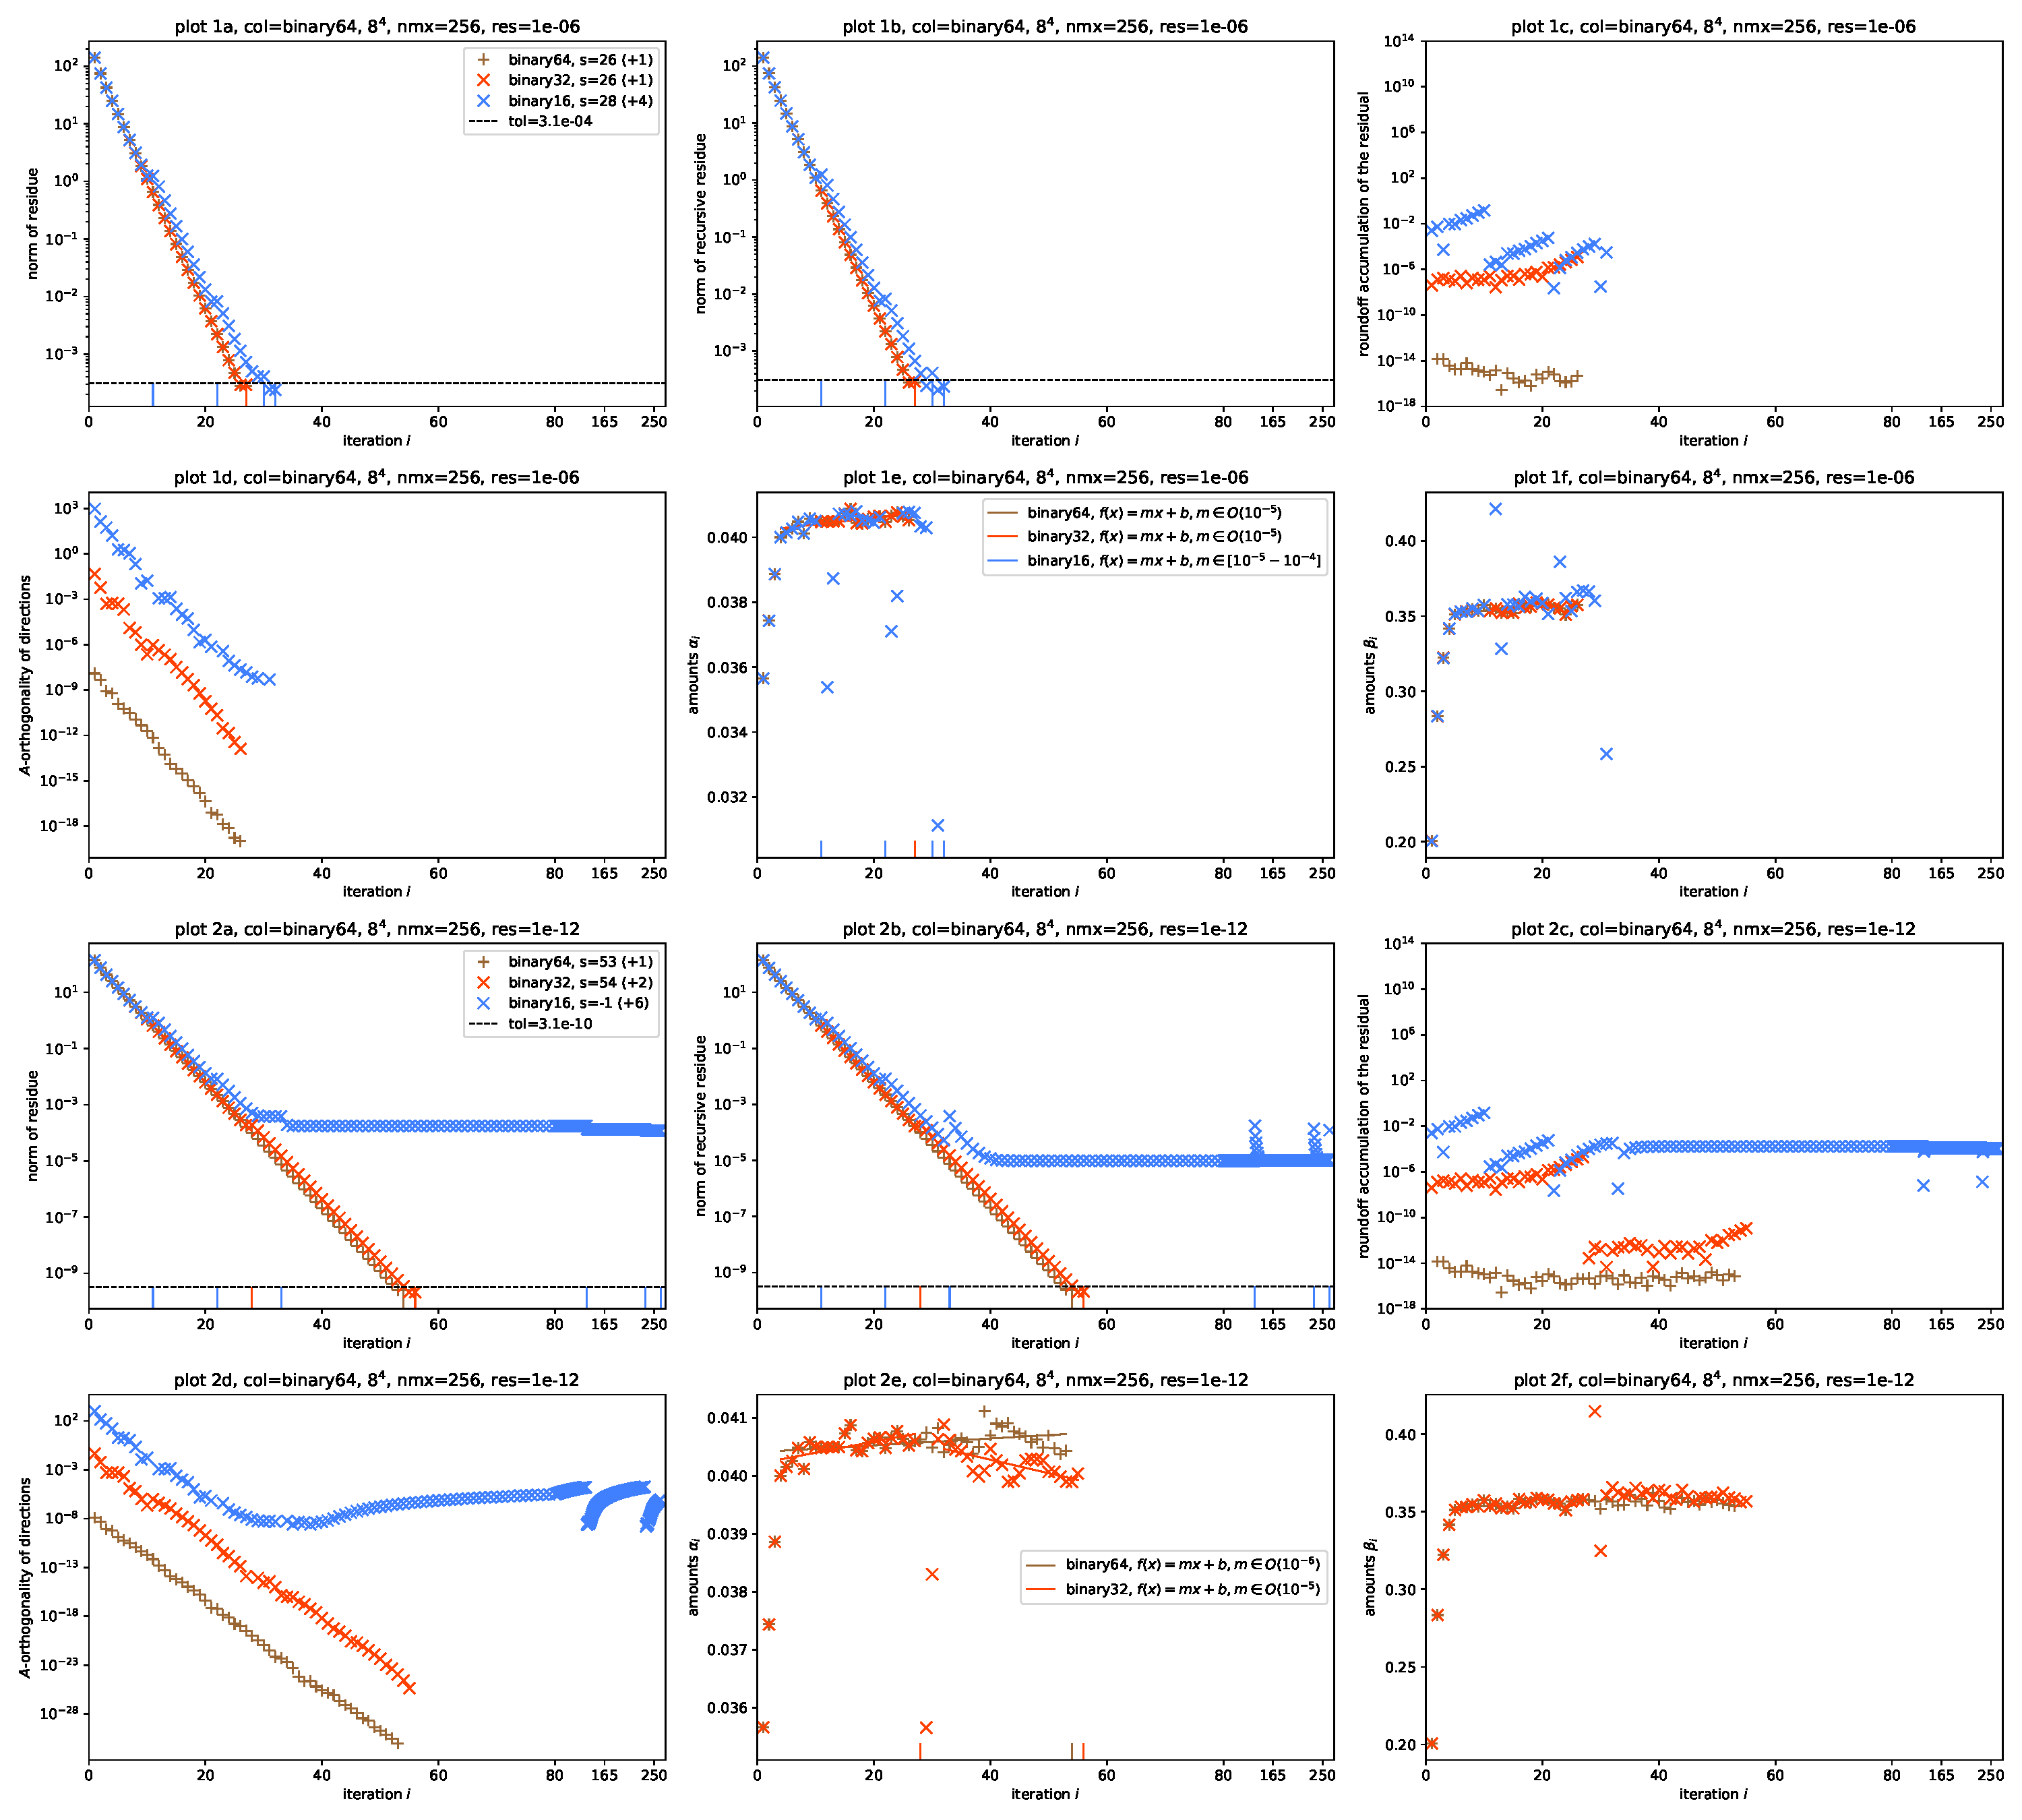
\includegraphics[width=1.0\textwidth]{plots/cgne_8x8x8x8_new}
    \caption{In analogy to figures \ref{fig:cgne:col64} and \ref{fig:cgne:res12}. This time an $8^4$ lattice was used and only the floating point datatypes that are available in hardware nowadays were simulated. The \textit{first and second row} use \gls{binary64} as collective variable and $10^{-6}$ was the desired relative residual. The \textit{third and fourth row} have the exact same setup, but with a relative residual of $10^{-12}$ instead.}
    \label{fig:cgne8}
\end{figure}

\subsubsection{Conclusion}

The decision between floats and posits is not trivial. It highly depends on how fast the machine can perform \acrshort{FLOPS} and \acrshort{POPS}. For example division in floating point arithmetic is very expensive (it may exceed \num{24} CPU cycles, many compiler optimisations evade them), whereas in posit arithmetic it is said to be cheap, because obtaining the inverse of a number is easy.

Another example could be that comparisons between floats are more expensive than for posits. Two posits are equal if their bit representations are equal. Comparing two floats is much more expensive, mainly because of the many \acrshortpl{nan} and since $0$ and $-0$ are equal but not bit-identical.

On the other hand, there is currently no hardware available, that has dedicated posit units and posits are not studied as intensive as floats. Floats are widespread, well understood and implemented in common hardware.

If one decides to replace \gls{binary32} with posits, the most elegant solution would be to naively replace the datatype and utilise \glspl{quire} in collective operations. To use \gls{binary64} collective variables is not recommended, because this would introduce many type conversions between the floating point and the posit format which is assumed to be expensive. The drawback of this method is that \gls{posit16} may only converge if the relative residue is chosen high enough (see plot \textit{2a} in Figure \ref{fig:cgne:quire}).

If the decision goes for floats, which might be the more realistic scenario, then the most elegant solution would be to use collective variables in \gls{binary64}. Type conversions between different IEEE floating point types are not considered to be expensive. The \gls{tensorfloat32} compared to \gls{binary32} and \gls{bfloat16} answers the question how important precision is in the calculation. All of them have the same number of exponent bits and therefore approximately the same number range, but very different precisions. We see that all of them were able to converge in any experiment, but with \gls{binary64} as collective variable, the results were closest to each other (see Figure \ref{fig:cgne:col64} plot \textit{3a}). The only real difference was in the amount of reset steps. If the datatype is lower in bit-length, the memory-boundedness suggests that the calculation performs faster, but the trade-off is the amount of (computationally expensive) reset steps that increases with less precision. However, the datatype for collective operations should be precise and should have a large number range. Since the amount of variables needed in that datatype does not scale with the lattice size, it is perfectly right to use a datatype with large bit-length. Comparing the convergence of \gls{bfloat16} in the naive case (Figure \ref{fig:cgne:naive} plot \textit{1a}) with the case \gls{binary64} collective variables (Figure \ref{fig:cgne:col64} plot \textit{3a}), it can be seen that the algorithm converged \num{21} steps faster, only because the collective datatype was chosen to be \gls{binary64}. On the other hand, comparing the performance of \gls{binary16} in the two plots, we see that the number range of the collective datatype brought \gls{binary16} from no convergence to convergence within \code{status=35} steps - only marginally slower than \gls{binary32}. These arguments make \gls{binary64} the best choice for variables with a collective role.

\begin{proposal}{Mixed Precision}{mp}

The above analysis suggests that the calculation of the solution can be (at least partly) conducted in an even less precise datatype than \gls{binary32}. One could for example choose \num{3} datatypes with different precision. The algorithm can be started using the least precise one. If the tolerance hits a certain value at the boundaries of the datatype, the algorithm switches to the next higher one. The calculation is continued in that datatype until the tolerance reaches the limits of the new datatype. Again the datatype is switched to the next higher one\footnote{One obvious choice could be $d = \{\text{binary64}, \text{binary32}, \text{binary16}\}$. When the algorithm is started in \gls{binary16} and a tolerance of $\approx 10^{-4}$ is reached, the algorithm continues in \gls{binary32}, the limit of which is at a tolerance of $\approx 10^{-35}$. A continuing calculation would then be conducted in \gls{binary64}.}. This calculation in mixed precision is not dependent on the algorithm itself and can therefore be applied to every iterative solver algorithm. Algorithm \ref{alg:mixed_precision} shows an example implementation of such a mixed precision calculation. The array $d$ consists of all available datatypes participating in the calculation in ascending order, meaning the least precise datatype comes first. The function $solve()$ performs the underlying algorithm (for example conjugate gradient) in the datatype given by its arguments. It expects at least a starting vector $\vec{x_0}$ and a tolerance and returns the status \footnote{See section \ref{sec:fp_in_openqxd}}, the calculated solution and the residual up to the given tolerance.

\begin{algorithm}[H]
\SetKwInOut{Input}{input}
\Input{desired norm of relative residual $rn$}
\Input{array of datatypes in $\{d\}_{k=0}^N$}
\Input{iterative algorithm $solve()$}
\SetAlgoLined
  $\vec{x_0}, \vec{r_0}, \ldots \gets$ initial guess, \ldots\;
  $\vec{x}, \vec{r} \gets \vec{x_0}, \vec{r_0}$\;
  status $\gets 0$\;
  \For{$k \gets 0, 1$ \KwTo $N$}{
    convert all variables to datatype $d[k]$\;
    $tol \gets \frac{1}{\norm{\vec{r_0}}} max(rn, \text{\code{MACHINE\_EPSILON of $d[k]$}})$\;
    substatus, $\vec{x}, \vec{r}$, $\ldots \gets solve(tol, \vec{x}, \ldots)$\;
    \uIf{substatus $> 0$}{
      status $\gets$ status $+$ substatus\;
    }
    \uIf{$\norm{\vec{r}} < rn$}{
      \Return status, $\vec{x};$ \tcp{success}
    }
 }
 status $\gets -3$\;
 \Return status, $\vec{x_0};$ \tcp{the algorithm failed}
 \caption{Pseudo-code for an iterative algorithm in mixed precision.}
 \label{alg:mixed_precision}
\end{algorithm}

\end{proposal}

\begin{proposal}{Approximating the amounts $\alpha_i$}{alpha}

Looking at plot \textit{4e} of Figure \ref{fig:cgne:res12}, where the amounts $\alpha_i$ are plotted for every iteration, we see that after every reset step the amounts need $2-3$ steps to reach a value that is not changing very much for future iterations. This is becomes apparent when looking at the fitting lines. The values of the $\alpha_i$ are in the range $10^{-1}$ and the slopes $m$ of the fitting lines are in the range $10^{-4}$ - $10^{-5}$, suggesting that the value of $\alpha_i$ is not changing from iteration to iteration when only looking at $2-3$ significant decimal digits.

A possibility to reduce computational cost in each iteration could be to approximate the values of future $\alpha_i$ to be constant. The less precise the datatype, the larger the change in $\alpha_i$. The large error in $\alpha_i$ of \gls{bfloat16} in all plots suggests that the algorithm is not sensible to errors in $\alpha_i$. Therefore, it can be expected that the results should not change significantly with a approximated value of $\alpha_i$.

\begin{itemize}
    \item Advantage: The residuals can be calculated using $\vec{b} - A \vec{x}$, not recursively. This implies less round-off accumulation.
    \item Advantage: Only one matrix-vector multiplication per iteration.
    \item Disadvantage: Since the $\alpha_i$ are just approximated, the number of needed iterations may increase.
    \item Disadvantage: The Dirac operator $D$ must be given in the form of $A = D^{\dagger} D$ as \textit{one} operator, else the algorithm still consists of \num{2} matrix-vector multiplications per iteration. Also, $D^{\dagger} D$ is less sparse than $D$.
\end{itemize}

The results of simulations with approximated values for the $\alpha_i$ can be observed in plot series \ref{fig:cgne:4x4x4x4:e1} and \ref{fig:cgne:8x8x8x8:e1}. The value was approximated based on previous values. The first \num{5} steps where skipped (thus the algorithm performed natively). In step number \num{5}, the last \num{3} values of $\alpha_i$ where averaged. In the following steps the constant value calculated in step \num{5} was reused. After every reset step, the value of $\alpha_i$ had to be recalculated using the above procedure. Therefore a datatype such as \gls{bfloat16} that has reset steps after approximately every \num{7}th regular step, will benefit in only \num{2} steps per reset step. This is very little difference to native runs compared to datatypes with high precision.

The calculation became more sensible to the number range of the datatype. This can be seen in all plots when looking at \gls{binary16} that was not able to converge anymore, although by a very small amount. \gls{tensorfloat32} on the other hand performed very similar to the regular rounds, it was expected that it needs slightly more iterations. When going with this strategy, it is therefore advisable to perform more regular cg-steps when coming closer to the boundaries of the datatype. One possible solution would be to choose a higher machine epsilon close to the boundaries, forcing the algorithm to perform more reset steps, in turn causing more regular cg-steps and recalculations of $\alpha_i$.

Notice that with larger lattice sizes, the approximation of the amounts has less error (see plots \textit{1e} and \textit{2e} in figures \ref{fig:cgne:4x4x4x4:e1} and \ref{fig:cgne:8x8x8x8:e1}) and the algorithm is thus more stable.

\end{proposal}

\begin{figure}
    \centering
    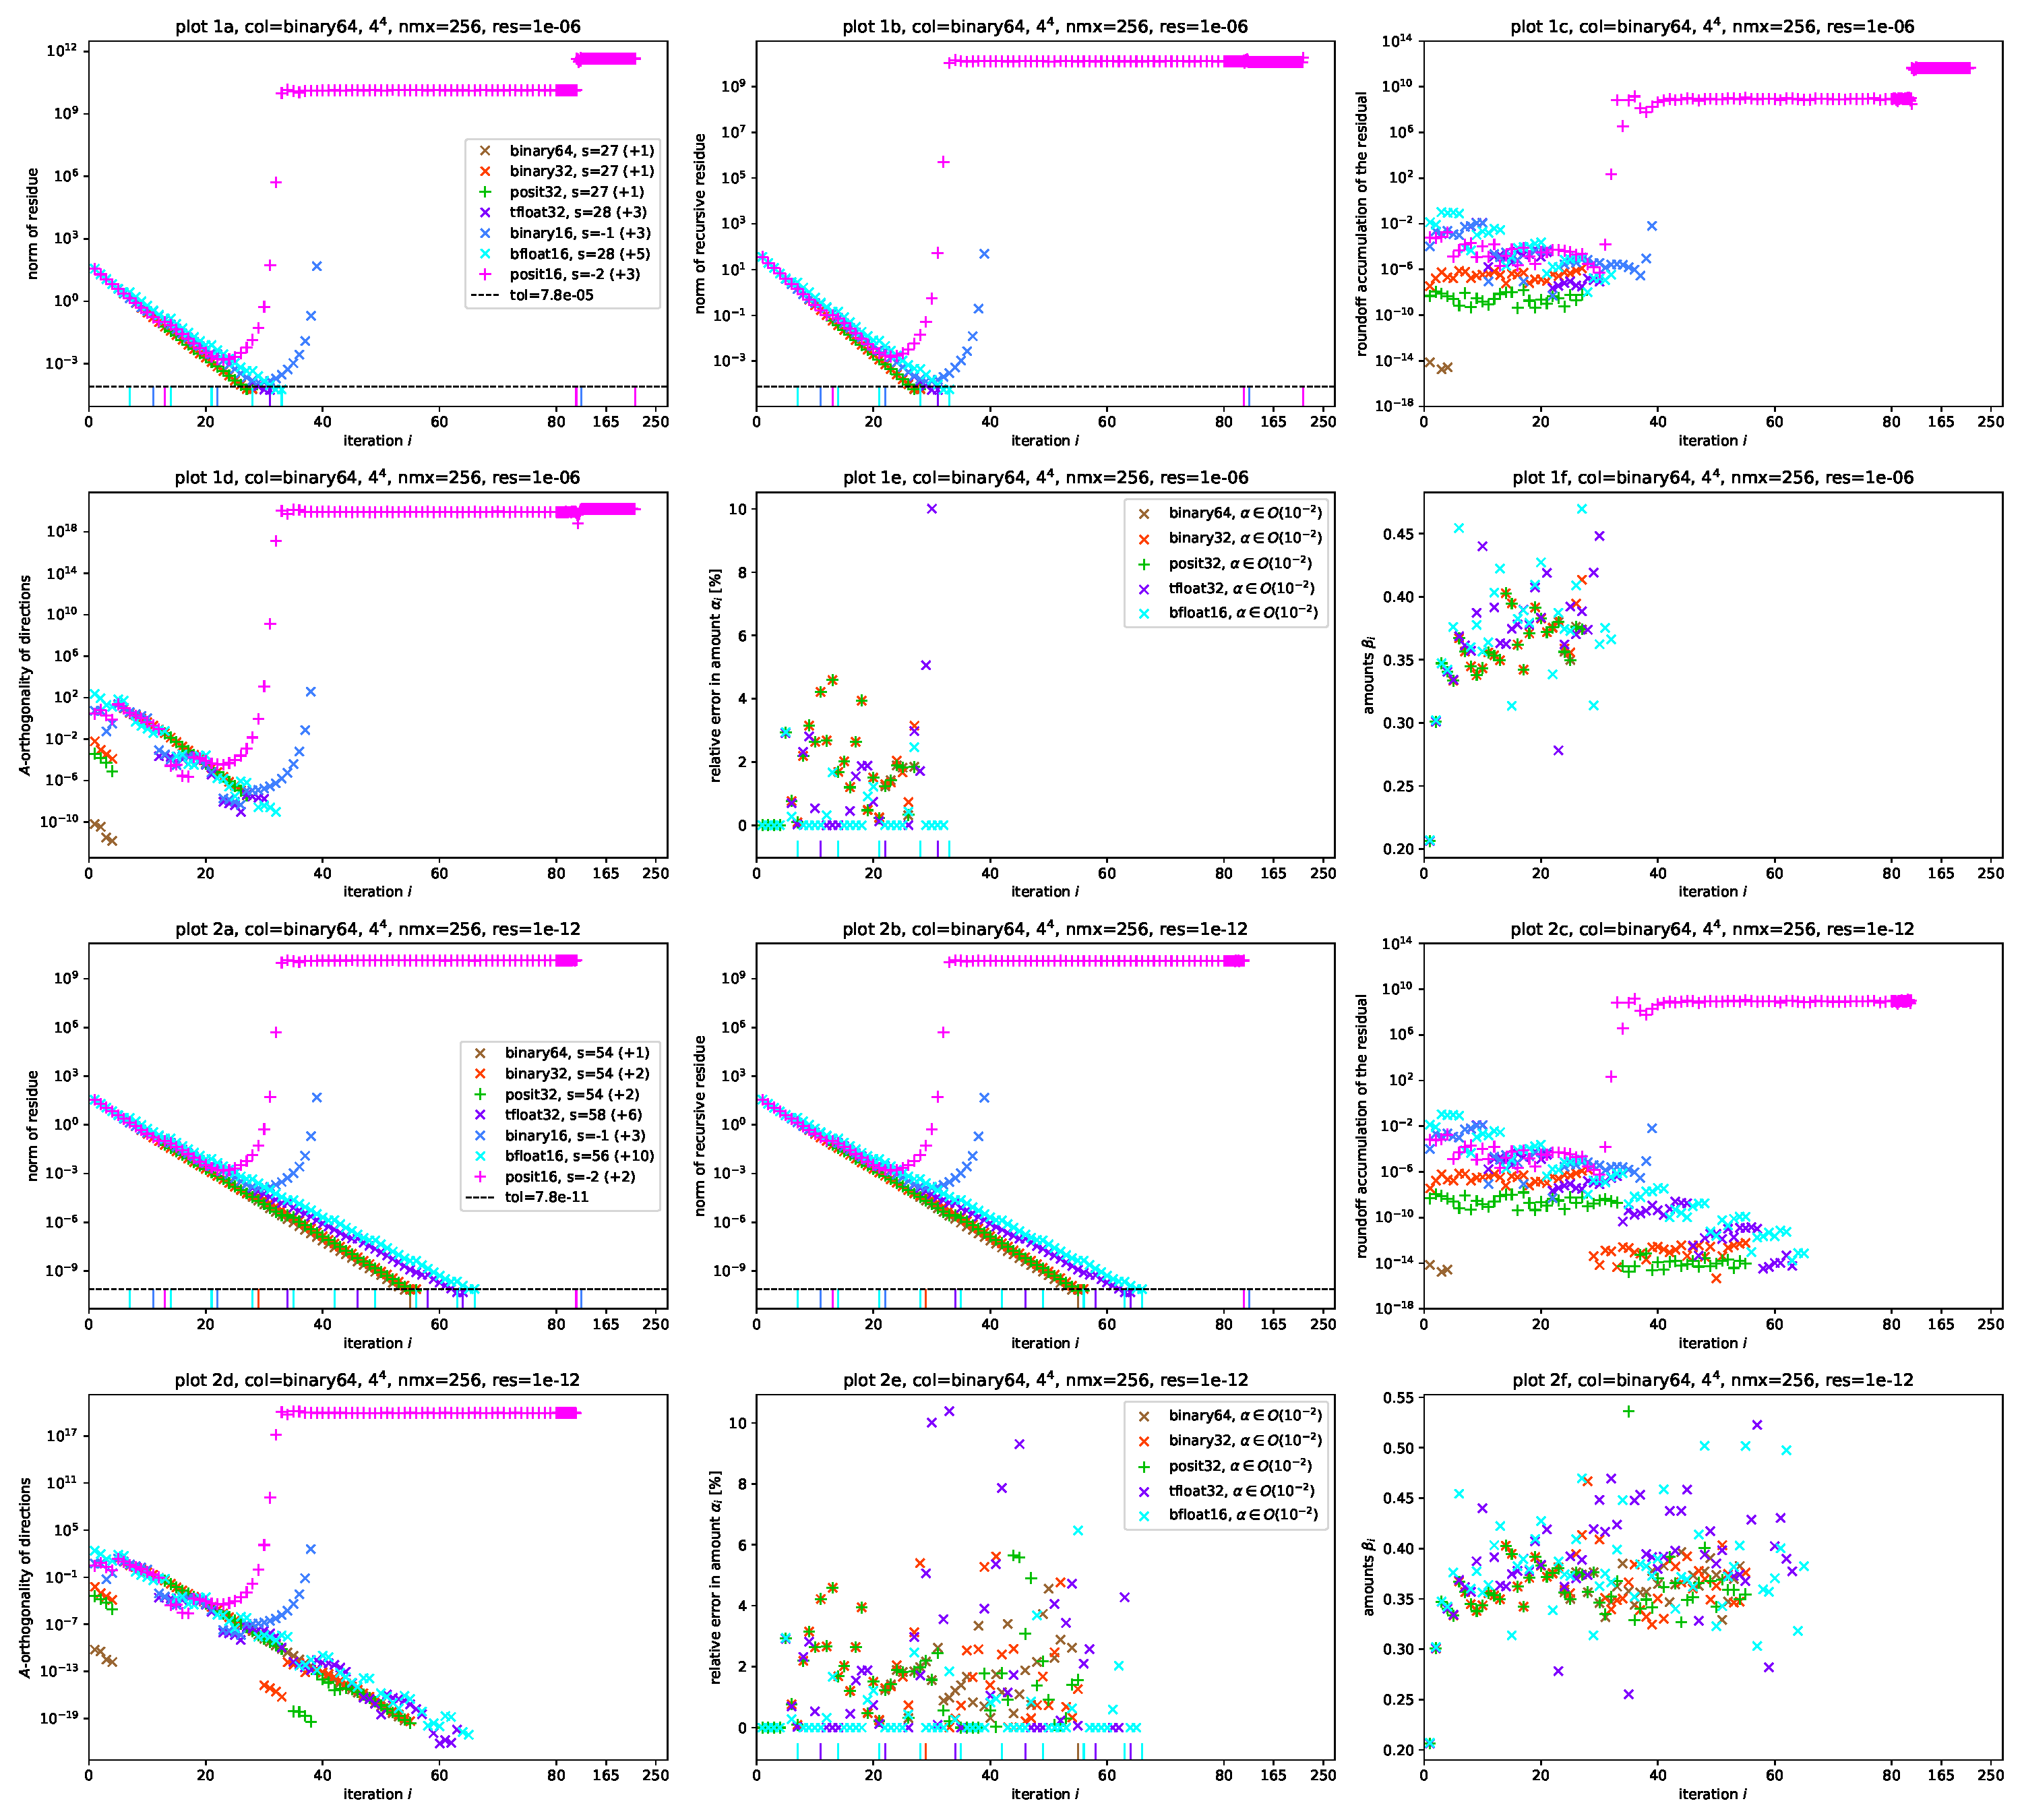
\includegraphics[width=1.0\textwidth]{plots/cgne_4x4x4x4_e1}
    \caption{Plots \textit{1a} to \textit{1f} contain the convergence analysis of a conjugate gradient run with a $4^4$ lattice, relative residual $10^{-6}$ and approximated values of $\alpha_i$. In plots \textit{2a} to \textit{2f} the residual was chosen to be $10^{-12}$. Plots \textit{1e} and \textit{2e} contain the relative error in the approximated $\alpha_i$ compared to the real $\alpha_i$.}
    \label{fig:cgne:4x4x4x4:e1}
\end{figure}

\begin{figure}[h]
    \centering
    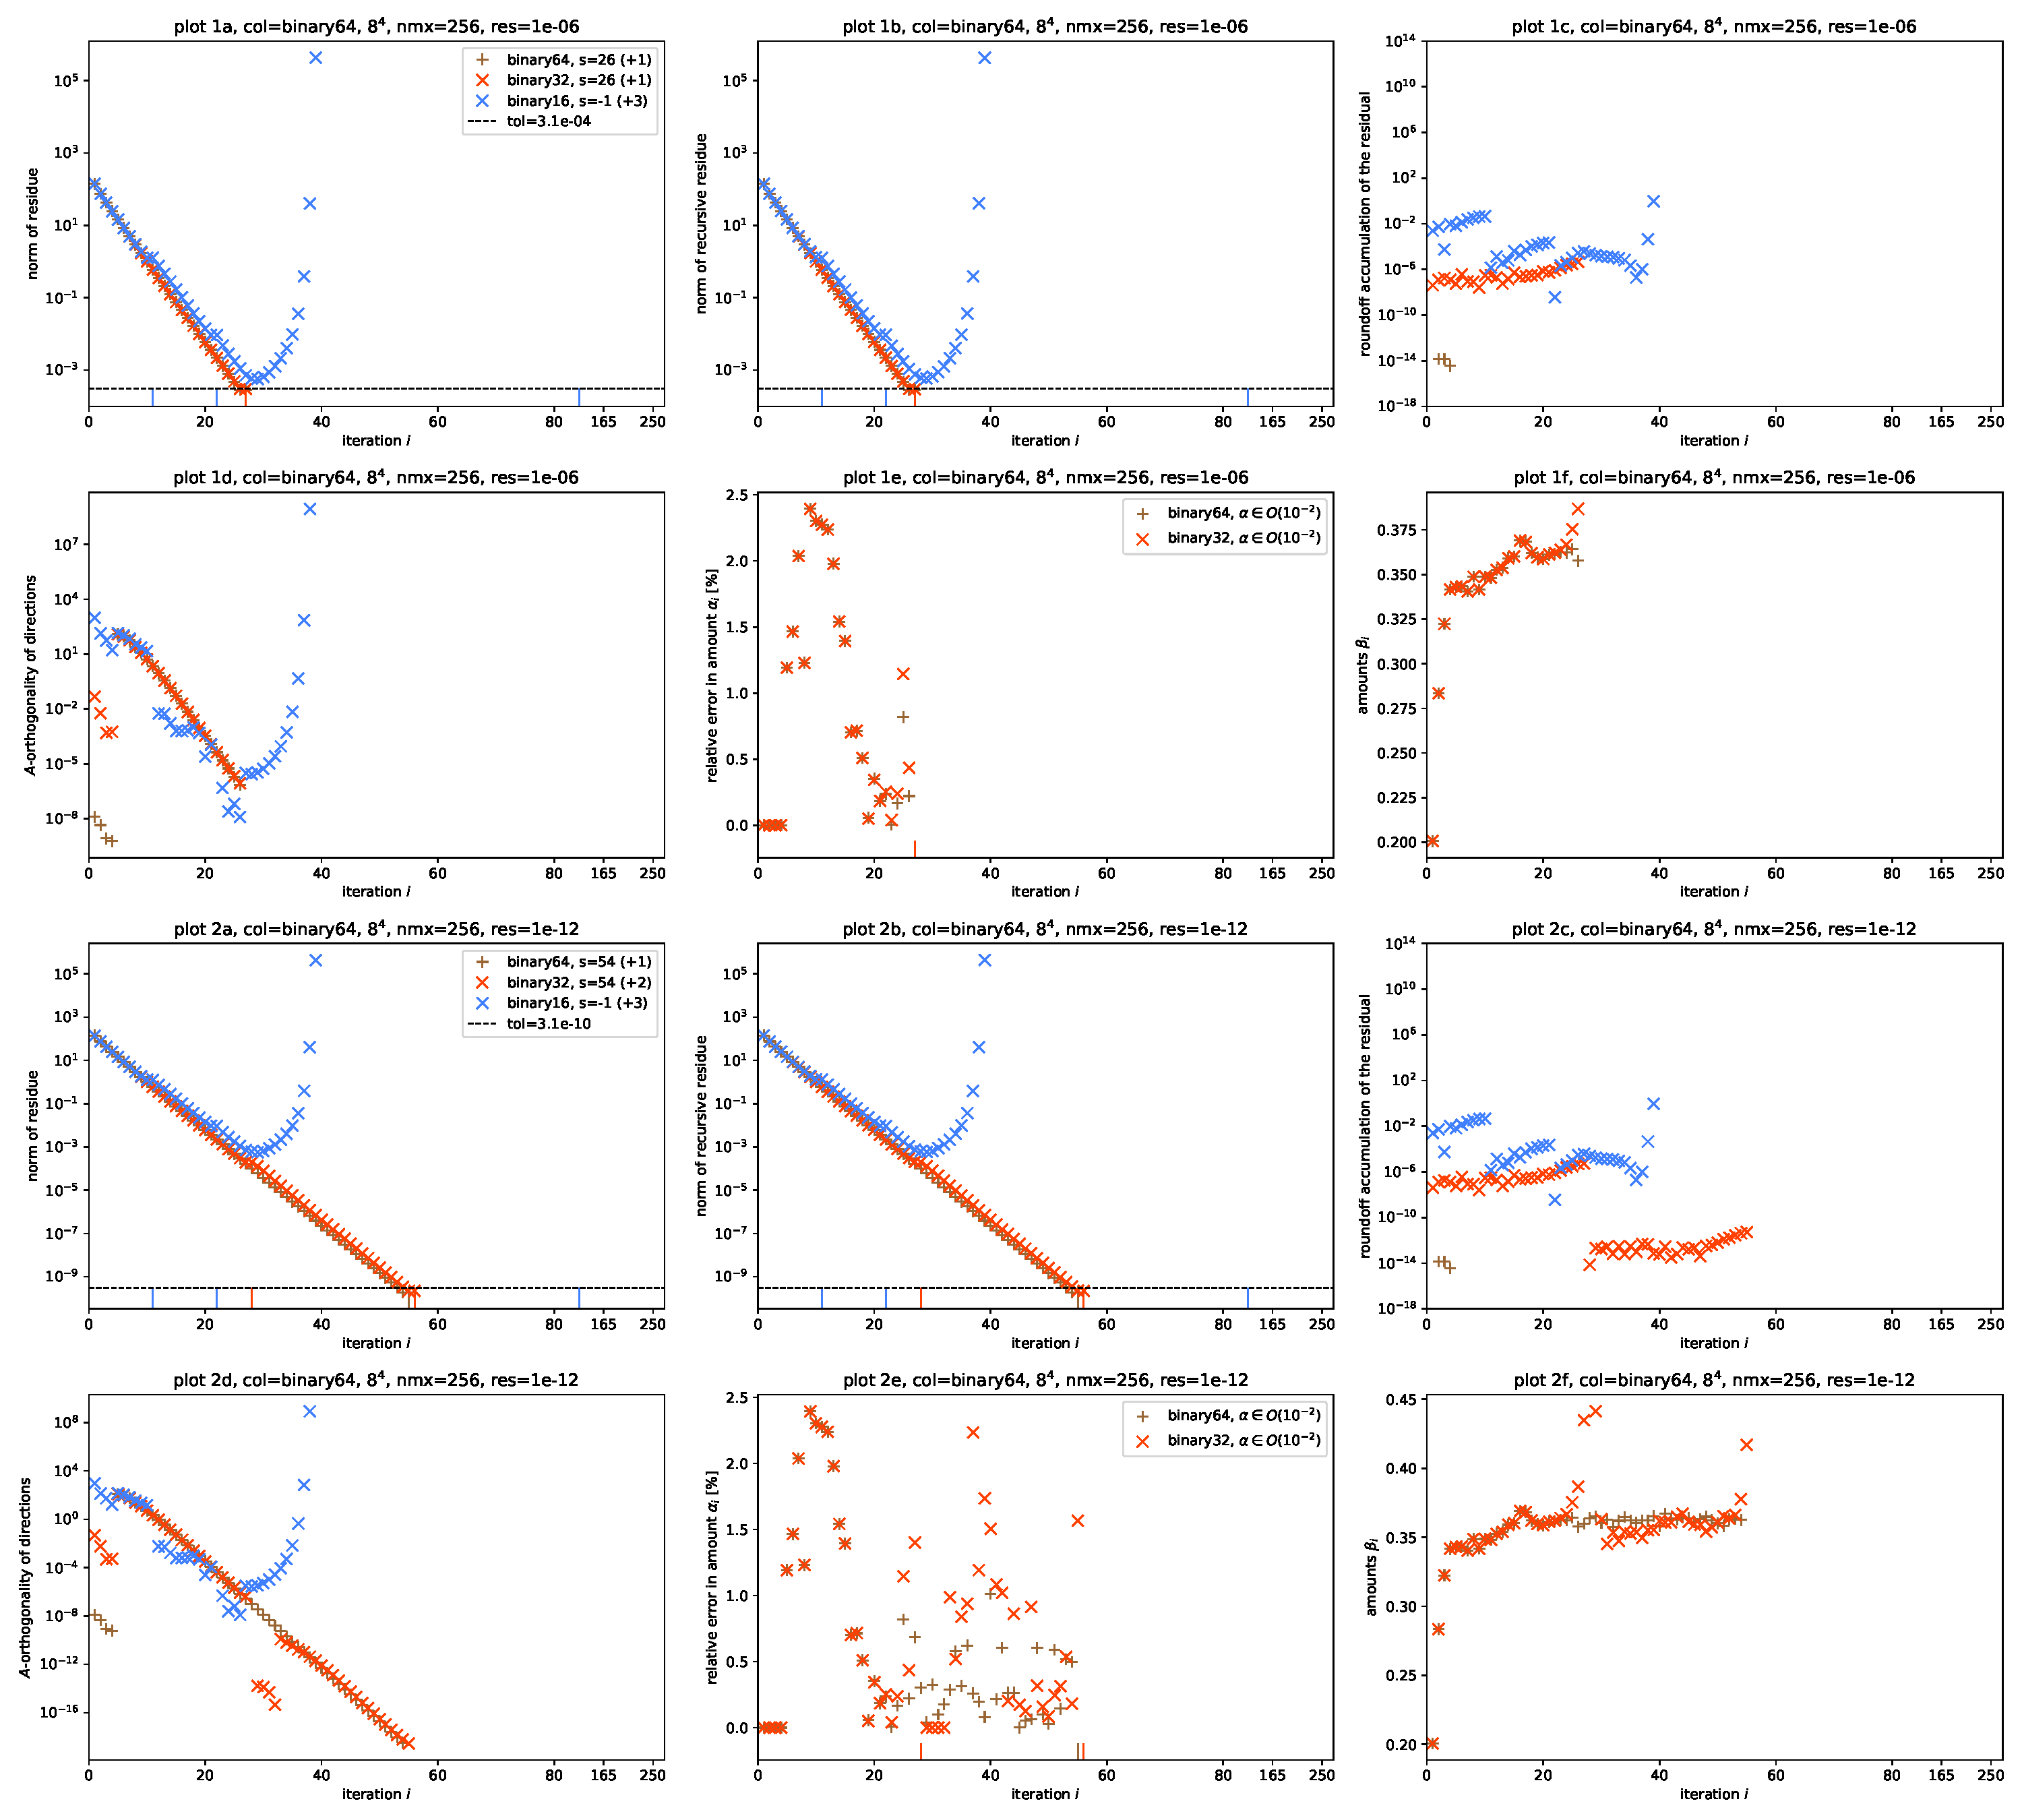
\includegraphics[width=1.0\textwidth]{plots/cgne_8x8x8x8_e1}
    \caption{The same setup as figure \ref{fig:cgne:4x4x4x4:e1}, but with a $8^4$ lattice.}
    \label{fig:cgne:8x8x8x8:e1}
\end{figure}

\begin{comment}

res $> 10^{-6}$

Simulated datatype: precision $>$ number range

Collective datatype: number range $>$ precision

res $< 10^{-6}$

Simulated datatype: precision $>$ number range

Collective datatype: number range $>$ precision

\end{comment}

\section{SAP preconditioned GCR algorithm}

The next solver appearing in openQxD is called \acrshort{sapgcr}. It makes use of a multiplicative \acrfull{sap} as preconditioner for a flexible \acrfull{gcr} run.

TODO: motivation: parallel processing, chiral regime (spontaneous breaking of chiral symmetry), simulation containing sea-quarks limited to small lattices and large quark masses.

\subsection{Even-Odd Preconditioning}

\begin{comment}

* Note that it works only because D(ee) is diagonal in space for Wilson (and Wilson-twisted) fermions.
* it does not allow “multisolvers” i.e. codes which solve different quark masses in one stroke (mscg).

\end{comment}

Preconditioning in general, when employed in lattice QCD, is expected to have significant impact on the number of iterations of a solver. One way of preconditioning $D \psi = \eta$ on a lattice is

\begin{align*}
    L D R \psi^{\prime} = L \eta,
\end{align*}

with $\psi = R^{-1} \psi^{\prime}$ and $L$, $R$ chosen wisely such that $LDR$ is well conditioned. If $L = \mathbb{I}$, it is called \df{right preconditioning}, if $R=\mathbb{I}$ it is called \df{left preconditioning}. If the Dirac-matrix involves only nearest-neighbour interactions it is possible to split the lattice into even and odd sites\footnotemark
\footnotetext{It is therefore very similar to a domain decomposition method, see later.}
\footnotemark.
\footnotetext{Even lattice points are the ones where the sum of the global Cartesian coordinates $(x_0 + x_1 + x_2 + x_3)$ in units of the lattice spacing $a$ is even.}
If the sites are ordered such that the even sites come first\footnotemark,
\footnotetext{This is indeed the case in openQxD (see \code{main/README.global}) in \cite{openqxd}.}

\begin{align*}
    D &=
    \begin{pmatrix}
    D_{ee} & D_{eo} \\
    D_{oe} & D_{oo}
    \end{pmatrix},
    & & &
    \psi &=
    \begin{pmatrix}
    \psi_e \\
    \psi_o 
    \end{pmatrix}
\end{align*}

$D_{ee}$ ($D_{oo}$) consists of the interactions of the even (odd) sites among themselves, whereas $D_{eo}$ and $D_{oe}$ consider the interactions of even with odd sites. $\psi_e$ and $\psi_o$ contain the values for even and odd lattice sites of the spinor.

Using specific forms of $L$ and $R$, $D$ can be brought in a block-diagonal form, namely

\begin{align*}
    L &= 
        \begin{pmatrix}
        1 & -D_{eo} D_{oo}^{-1} D_{oe} \\
        0 & 1
        \end{pmatrix}
    & &\text{and} &
    R &= 
        \begin{pmatrix}
        1 & 0 \\
        -D_{oo}^{-1} D_{oe} & 1
        \end{pmatrix}.
\end{align*}

After a bit of algebra,

\begin{align*}
    L D R &= 
        \begin{pmatrix}
        \hat{D} & 0 \\
        0 & D_{oo}
        \end{pmatrix},
    & &\text{with} &
    \hat{D} &= D_{ee} - D_{eo} D_{oo}^{-1} D_{oe}.
\end{align*}

This specific preconditioning reduces the amount of iterative steps needed by a factor of \num{2} approximately, because $D_{oo}$ and $\hat{D}$ are matrices of half the dimension of $D$. The inversion of $D_{oo}$ is simple, because with only nearest-neighbour-interactions the odd sites do not interact among themselves, only with even sites. Thus $D_{oo}$ exhibits block-diagonal form (all blocks are $6 \times 6$, why?). Using

\begin{align*}
    D \psi = \eta \implies \begin{pmatrix}
    D_{ee} & D_{eo} \\
    D_{oe} & D_{oo}
    \end{pmatrix} \begin{pmatrix} \psi_e \\ \psi_o \end{pmatrix} = \begin{pmatrix} D_{ee} \psi_e + D_{eo} \psi_o \\ D_{oe}\psi_e + D_{oo} \psi_o \end{pmatrix} = \begin{pmatrix} \eta_e \\ \eta_o \end{pmatrix}
\end{align*}

we can write the preconditioned form, where only the reduced system with even lattice sites has to be solved to determine $\psi_e$

\begin{align*}
    \hat{D} \psi_e &= D_{ee} \psi_e - D_{eo} D_{oo}^{-1} D_{oe} \psi_e \\
    &= ( \eta_e - D_{eo} \psi_o ) - D_{eo} D_{oo}^{-1} ( \eta_o - D_{oo} \psi_o ) \\
    &= \eta_e - D_{eo} D_{oo}^{-1} \eta_o,
\end{align*}

because $\psi_o$ follows from the solution $\psi_e$ via

\begin{align*}
    \psi_o = D_{oo}^{-1} (\eta_o - D_{oe} \psi_e).
\end{align*}

\subsection{Schwarz Alternating Procedure}

\label{sec:ddecomp}

Domain decomposition is a way to partition the large system into (possibly many) smaller sub-problems with regularly updated boundary conditions coming from solutions of neighbouring sub-problems. They fit very well into the notion of parallel processing, because the sub-problem can be chosen to be contained in one single rank. The full lattice is split into sub-lattices called \df{local lattice}. Each rank has its own local lattice, the size of which is determined at compilation time. The full lattice consists of the ensemble of all local lattices arranged in a grid. It is therefore advisable to choose the size of decomposed sub-domains as a divisor of the local lattice size such that one or more blocks fit into one rank. These sub-problems can then be solved using a iterative solving method.

\begin{figure}[h]
  \centering
  %\includestandalone[]{schemes/domain_decomposition}
  \subimport{schemes/}{domain_decomposition}
  \caption{$d=2$ dimensional example of a decomposition of a lattice $\Omega$ into domains named $\Omega_i$.}
  \label{fig:ddecomp}
\end{figure}

The idea behind \acrshort{sap} is to loop through all blocks $\Omega_i$ and solve the smaller sub-problem using boundary conditions given from the most recent global solution (see figure \ref{fig:ddecomp}). If the original problem only includes nearest-neighbour interactions, the solution of a block $\Omega_i$ depends only on that block and its exterior boundary points, which are the adjacent points on the neighbouring blocks with opposite color. For example, the solution of the sub-problem involving $\Omega_6$, depends only on the solutions of $\Omega_2$, $\Omega_5$, $\Omega_7$ and $\Omega_{10}$\footnotemark.
\footnotetext{It depends on all other sub-problems as well, but only indirectly.}
Therefore all gray (white) sub-problems can be solved simultaneously, with the most recent boundary conditions obtained from the white (gray) domains. Solving all gray, followed by all white sub-problems is called a \df{Schwarz cycle} and is considered one iteration in the \acrshort{sap}. Each sub-problem can be solved with a desired solver separately, again applying some preconditioning\footnotemark.
\footnotetext{Using even-odd preconditioning is perfectly fine with $D$ replaced by the restricted Dirac operator $D_i$ acting only on the points in $\Omega_i$.}

\begin{figure}[h]
    \centering
    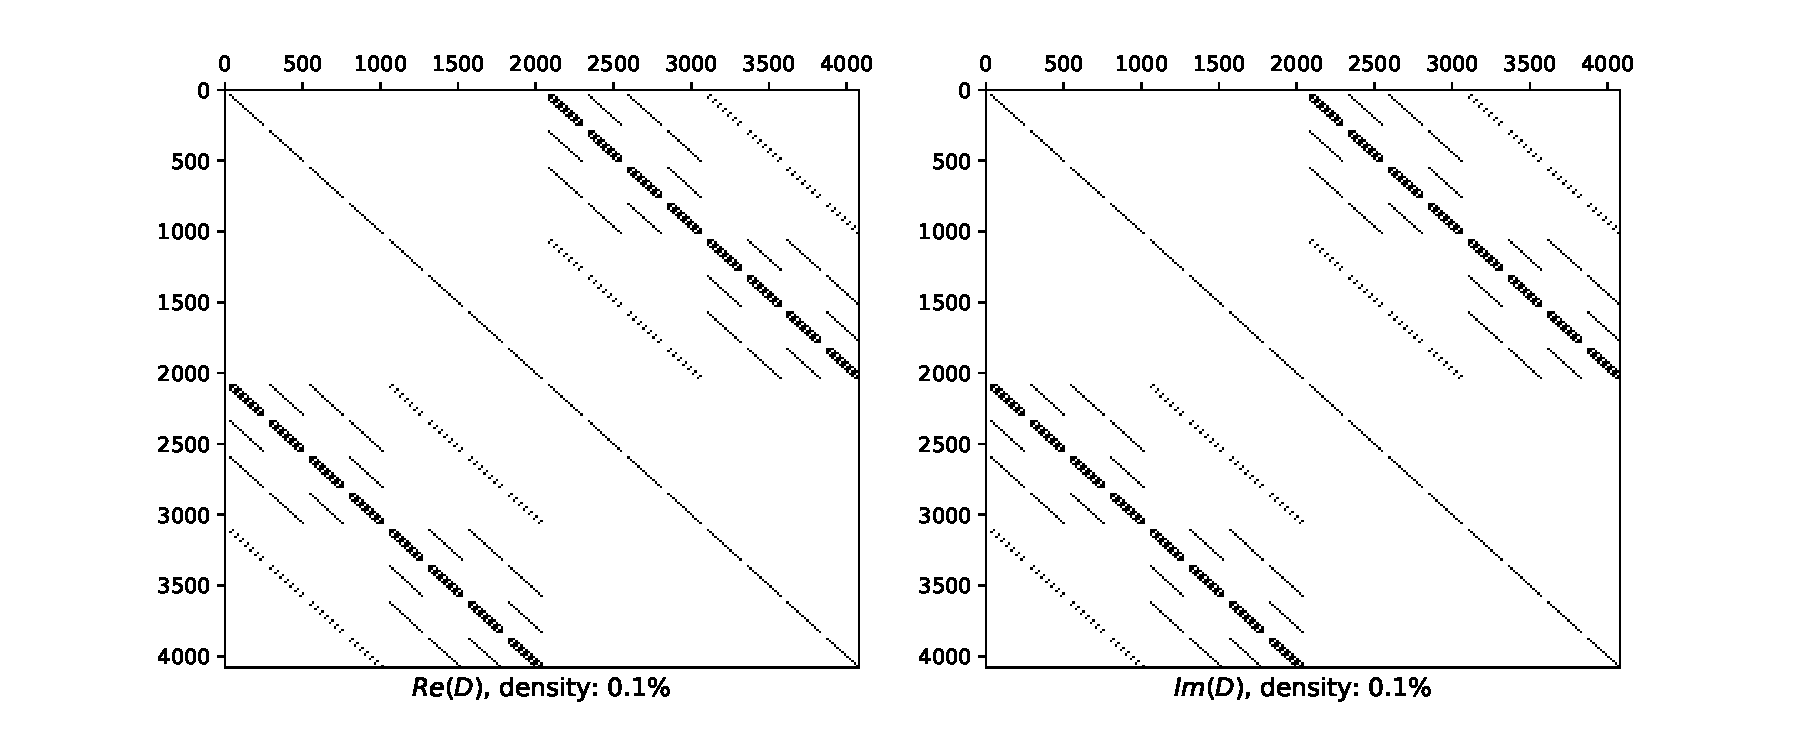
\includegraphics[width=1.0\textwidth]{plots/dirac_matrix6}
    \caption{An example plot of a Dirac-matrix of an $8^4$-lattice with \acrshort{sf}-boundary conditions. Every pixel consists of $192 \times 192$ real numbers. If the average over that numbers is non-zero the pixel is drawn black, else the pixel is drawn white. The density states the percentage of non-zero values over all entries.}
    \label{fig:dirac_matrix}
\end{figure}

Whereas the division into domains on the lattice is straightforward, the representation of the Dirac-operator as a sparse matrix and its decomposition is not. Looking at an actual example of a Dirac-operator as matrix (see figure \ref{fig:dirac_matrix}), one observes a lot of structure. While on the diagonal we find the operators restricted to the black and white blocks, the first and the third quadrant describe the operators restricted to the interior and exterior boundaries of the blocks. The operator restricted to the exterior boundaries of the union of all black (white) blocks is denoted by $D_{\partial b}$ ($D_{\partial w}$). The decomposition into $2n$ domains ($n$ gray and $n$ white blocks) can be translated as seen in figure \ref{fig:ddecomp_matrix}. Notice that the restricted operators $D_i$ are well-conditioned, because they exhibit block diagonal form. The blocked problem would then look like, $i = 1, \dots, 2n$,

\begin{align*}
    D_i \psi_i = \eta_i.
\end{align*}

\begin{figure}[h]
  \centering
  %\includestandalone[]{schemes/dd_matrix}
  \subimport{schemes/}{dd_matrix}
  \caption{Schematic of the Dirac-operator in term of a large sparse matrix. If the components of the black blocks are arranged such that they appear first, then the decomposition from figure \ref{fig:ddecomp} can be translated into a matrix with blocks as in the picture. $D_i$ describes the Dirac-operator restricted to block $i$ and $D_{\partial b}$ ($D_{\partial w}$) is the Dirac-operator restricted to the external boundaries of the black (white) blocks. The color external boundary operators can be decomposed into external boundary operators of the $i$-th block; $D_{\partial^{*}_i}$. The right side describes a vector decomposed into the same $2n$ domains $\psi_1, \dots, \psi_{2n}$. The upper half corresponds to the black blocks and the lower half to the white blocks.}
  \label{fig:ddecomp_matrix}
\end{figure}


\begin{comment}
TODO: formulate the block sub-problem here, and the sap cycle. D only couples nearest-neighbour blocks, see (0706.2298 Local coherence and deflation of the low quark modes in lattice QCD Fig.4)

kappa, the lattice hopping term, determines to how many neighbours the interactions are extended.
the wilson dirac operator D_w in doc/dirac.pdf eq (10) has only nearest neighbour interactions
\end{comment}

\subsection{SAP as a Preconditioner}

\begin{comment}

No overlapping (why?) of domains, as preconditioner (why?)

Before calling GCR, calculate the P_i and T_i (Saad Page 490), i-th operator for i-th rank.
Then calc M^-1 b using the T_i simultaneously on all ranks
Start GCR
In each GCR step: M^-1 A x_i must be calculated, using the P_i on all ranks simultaneously.
M^-1 is the preconditioner that is not explicitly available, only implicitly via the P_i. However the M^-1 is not an exact inverse of A, but approximates A^-1. The remaining matrix B = M^-1 A is "close" to the identity, which makes Bx=c solved in very few steps, with c=M^-1b.

The domain decomposition preconditioner based on \acrshort{sap} involves itself an iterative procedure and is therefore very expensive.

* fixed number of GMRES iterations can be a preconditioner as well
* choice of preconditioner is often more important than the choice of iterative method [Yousef Saad book]
* preconditioning = bringing the condition number of a matrix closer to 1 (cond(id) = 1)

The block sizes bs[4] and other parameters of the specified block grid
are obtained from the parameter data base. These and the lattice sizes
must be such that the lattice can be covered by non-overlapping blocks.
Moreover, the number of blocks in each direction must be even and the
local lattices must contain an even number of blocks. This ensures that
the block grid can be chessboard-coloured and that the number of blocks
in the local lattice is the same for both colours.

The blocks are ordered such that the first half of them have the same colour (black by definition).

\end{comment}

The multiplicative \acrlong{sap} is such a domain decomposition method coming from the theory of partial differential equations. It can be applied in the form of a right preconditioner $M^{-1}$ making the preconditioned system

\begin{align}
    M^{-1} A \vec{x} = M^{-1} \vec{b} \label{eq:sap:preconditioned}
\end{align}

to be solved in very few steps, if $M^{-1}$ is a good approximation for $A^{-1}$. The preconditioning matrix $M^{-1}$ although is never explicitly available during the calculation, such as it is the case in even-odd preconditioning which can also be applied in advance. In order to solve the preconditioned equation \eqref{eq:sap:preconditioned} using a iterative Krylov subspace method, the algorithm must be able to apply $M^{-1}$ and $M^{-1} A$ to an arbitrary vector $\vec{v}$. If it is possible to implement such operations on multiple ranks in an efficient way and if the preconditioner makes $M^{-1} A$ well conditioned\footnotemark, we reached the goal.
\footnotetext{Would it be dingy to expect such a thing from a preconditioner?}
Obviously an application of $M^{-1}$ should be possible without involving $A^{-1}$. The actions of operators $M^{-1}$ and $M^{-1} A$ on a vector $\vec{v}$ are assembled using a multiplicative \acrlong{sap}, where the blocks are treated by some fixed number of \acrfull{mr} steps\footnotemark. The blocks need not to be solved to a certain precision, because the procedure is only used as a preconditioner approximating the solution. This is a motivation for proposal \ref{pp:sap_reduced_precision}.

\footnotetext{Determined by the value of \code{mnr} in the solver section of the input file.}

In openQxD the \code{SAP\_GCR} solver is implemented as follows: The large problem is solved using a flexible \acrshort{gcr} solver, that in each of its \code{nmx} steps uses a different preconditioner. The preconditioner is given by \code{ncy} steps of the \acrlong{sap} applied to the current solution vector. Each \acrshort{sap} cycle involves approximately solving all gray followed by all white blocks on the whole lattice each with \code{nmr} steps of the \acrshort{mr} method using even-odd preconditioning (\code{isolv=1}) or not (\code{isolv=0}).

\begin{proposal}{MR in reduced precision}{sap_reduced_precision}

%\label{pp:sap_reduced_precision}

Since \acrshort{mr} is memory-bound, it can be conducted in mixed or reduced precision.

\begin{comment}
TODO: sap as preconditioner does not have to be precise, only approximation, thus reduced precision in the calculations? Is sap-preconditioning memory-bound? Involves network communication as well on the surface, therefore surface to volume ratio should be as small as possible, meaning the SAP-blocks should be as large as possible. Trade-off: reduced precision performs better with small blocks, but network communication is minimised with large blocks.
EO-reconditioning also in reduced precision?
\end{comment}

\end{proposal}

\begin{proposal}{Performing the MR steps on the GPU}{sap_mr_gpu}

The preconditioning procedure involves \code{mnr} \acrfull{mr} steps to be taken on each block in each Schwarz cycle to approximate a solution to the block problem. Since blocks of the same color are independent on each other and the Dirac operator acting only on a specific block involves no communication whatsoever, we can conclude that the procedure of solving a sub-problem is a problem \textit{local} to the block and self-contained in the sense that it can be solved independently and without MPI communication among ranks. This could be a very handy starting point when going towards GPU-utilisation. Once the source vector and the restricted Dirac operator are transferred to the GPU (both stay constant during the solving process), the problem can be solved on the GPU without involving any communication with other ranks or GPUs. This can also be beneficial, because of the following argument: The local lattice of one single rank, can be subdivided into multiple blocks as well (imagine figure \ref{fig:ddecomp} being the local lattice). The actual implementation solves the gray (white) blocks in a local lattice sequentially\footnote{By iterating over the blocks, see \code{sap()} at line \num{717}ff in \code{modules/sap/sap.c} in \cite{openqxd}.}. Since all the gray (white) problems within the local lattice can be solved simultaneously, the code does not exploit the full concurrency potential of the procedure. Solving the sub-problems on the GPU, one could launch \acrshort{mr} solvers on all gray blocks simultaneously followed by all white blocks. Keeping in mind proposal \ref{pp:sap_reduced_precision}, the \acrshort{mr} solver can be called in mixed or even reduced precision.

For a specific implementation of the GPU-solver, one option is to encode the restricted Dirac-operator in one of the sparse matrix formats (for example \acrshort{csr}) and use already existing libraries (for example \cite{bell2008} for \acrshort{cuda}) for an application to a spinor. Comparing the implementation of the Dirac-operator in QUDA (see ref. \cite{clark2010}), it is advisable to not rely on such generic libraries, because they ignore further symmetries and structure of the operator. The problem lies mostly in the memory-boundedness of the procedure.

\end{proposal}

\subsection{Generalised Conjugate Residual algorithm}

TODO: Why GCR? it allows inexact preconditioning without compromising the correctness of the solution.

We wish to solve \eqref{eq:Axb} if $A$ is not Hermitian. Comparing to the conjugate gradient algorithm, we minimise the residual $\vec{r}$ of the solution $\vec{x}$, using the \df{quadratic form},

\begin{align*}
    f(\vec{x}) &= \frac{1}{2} \left( \vec{b} - A \vec{x} \right)^{\dagger} \left( \vec{b} - A \vec{x} \right) + c \\
               &= \frac{1}{2} \norm{ \vec{b} - A \vec{x} }^2 + c\\
               &= \frac{1}{2} \norm{ \vec{r} }^2 + c.
\end{align*}

where $c \in \mathbb{C}$. When taking the derivative of this function with respect to $\vec{x}$, we find that

\begin{align*}
    f'(\vec{x}) = A^{\dagger} A \vec{x} - A^{\dagger} \vec{b}.
\end{align*}

\begin{lemma}[Uniqueness of the solution]
The solution $\vec{x}$ in equation \eqref{eq:Axb} is unique and the global minimum of $f(\vec{x})$, if $A$ is non-singular.
\end{lemma}

\begin{proof}
Let us rewrite $f(\vec{p})$ at an arbitrary point $\vec{p} \in \mathbb{C}$ in terms of the solution vector $\vec{x}$,

\begin{align*}
    f(\vec{p}) &= \frac{1}{2} \left( \vec{b} - A \vec{p} \right)^{\dagger} \left( \vec{b} - A \vec{p} \right) + c + f(\vec{x}) - f(\vec{x}) \\
    &= f(\vec{x}) + \frac{1}{2} \vec{p}^{\dagger} (A^{\dagger} A) \vec{p} - \frac{1}{2} (A \vec{p})^{\dagger} \vec{b} - \frac{1}{2} \vec{b}^{\dagger} (A \vec{p}) + \frac{1}{2} \vec{b}^{\dagger} \vec{b} \\
    &= f(\vec{x}) + \frac{1}{2} (\vec{p} - \vec{x})^{\dagger} (A^{\dagger} A) (\vec{p} - \vec{x}) + \frac{1}{2} (A \vec{p})^{\dagger} (\textcolor{cyellow}{A \vec{x}}) + \frac{1}{2} (\textcolor{cyellow}{A \vec{x}})^{\dagger} (A \vec{p}) - \frac{1}{2} (\textcolor{cyellow}{A \vec{x}})^{\dagger} (\textcolor{cyellow}{A \vec{x}}) \\
    &\phantom{==} - \frac{1}{2} (A \vec{p})^{\dagger} \textcolor{cyellow}{\vec{b}} - \frac{1}{2} \textcolor{cyellow}{\vec{b}}^{\dagger} (A \vec{p}) + \frac{1}{2} \textcolor{cyellow}{\vec{b}}^{\dagger} \textcolor{cyellow}{\vec{b}} \\
    &= f(\vec{x}) + \frac{1}{2} (\vec{p} - \vec{x})^{\dagger} (A^{\dagger} A) (\vec{p} - \vec{x}) \\
\end{align*}

where to obtain the last line, $\textcolor{cyellow}{A \vec{x}} = \textcolor{cyellow}{\vec{b}}$ as used, thus the term simplified.

In the new form of $f(\vec{p})$, one can directly see that, $\vec{x}$ must minimise the function:

\begin{align*}
    f(\vec{p}) &= f(\vec{x}) + \frac{1}{2} (\vec{p} - \vec{x})^{\dagger} (A^{\dagger} A) (\vec{p} - \vec{x}) \numberthis \label{eq:fp_gcr} \\
    &= f(\vec{x}) + \frac{1}{2} \underbrace{ \norm{ A (\vec{p} - \vec{x})}^2 }_{\text{$> 0$ for $\vec{p} \neq \vec{x}$}}.
\end{align*}

Therefore $\vec{x}$ is the global unique minimum if $A$ is non-singular.

\end{proof}

\begin{remark}
Notice the similarity of the above equation \eqref{eq:fp_gcr} to the analogue of the conjugate gradient algorithm \eqref{eq:fp_cgne}. The only difference is the substitution of $A \longmapsto A^{\dagger} A$. It is therefore advisable in the derivation of an algorithm to require the directions $\vec{p}_i$ to be $A^{\dagger} A$-orthogonal instead of $A$-orthogonal.
\end{remark}

In the same manner as in the derivation of the method of conjugate gradient, we impose a iterative \df{step equation} to be

\begin{align*}
    \vec{x}_{i+1} = \vec{x}_i + \alpha_i \vec{p}_i,
\end{align*}

again with \df{directions} $\vec{p}_i$ and \df{amounts} $\alpha_i$ that have to be determined. The recursively calculated \df{residual} has again the same formula

\begin{align*}
    \vec{r}_{i+1} = \vec{r}_i - \alpha_i A \vec{p}_i.
\end{align*}

Imposing $A^{\dagger} A$-orthogonality instead of regular $A$-orthogonality between error $\vec{e}_{i+1}$ and direction $\vec{p}_i$,

\begin{align*}
    0 &\stackrel{!}{=} \vec{e}_{i+1}^{\dagger} (A^{\dagger} A) \vec{p}_i \\
                    &= ( \vec{e}_{i} + \alpha_i \vec{p}_i )^{\dagger} A^{\dagger} A \vec{p}_i \\
\end{align*}

gives an expression for the amounts $\alpha_i$. Notice the above equation is equivalent to imposing $A$-orthogonality $0=\vec{r}_{i+1}^{\dagger} A \vec{p}_i$. However, we find (compare equation \eqref{eq:cgne:alpha_pre})

\begin{align*}
      \alpha_i = \frac{ \vec{r}_i^{\dagger} (A \vec{p}_{i}) }{ \vec{p}_i^{\dagger} (A^{\dagger} A) \vec{p}_i } = \frac{ \vec{r}_i^{\dagger} (A \vec{p}_{i}) }{ \norm{A \vec{p}_i}^2 }.
\end{align*}

The \acrshort{gcr} algorithm does store all previous direction $\vec{p}_i$ as well as $A \vec{p}_i$ in contrast to conjugate gradient. Thus the derivation changes slightly. Let's continue with the determination of the directions using \df{Gram-Schmidt orthogonalization} by imposing $A^{\dagger} A$-orthogonality instead of $A$-orthogonality and without imposing all previous $\beta_{ij}$ to be zero (see definition \ref{df:gramschmidt}). Likewise, we set $\vec{u}_i = \vec{r}_i$ and find

\begin{align*}
    \begin{split}
        \vec{p}_0 &= \vec{r}_0 \\
        \vec{p}_{i+1} &= \vec{r}_{i+1} + \sum_{j=0}^{i} \beta_{ij} \vec{p}_j,
    \end{split}
\end{align*}

with

\begin{align*}
    \beta{ij} = - \frac{ \vec{r}_{i+1}^{\dagger} A^{\dagger} A \vec{p}_j }{ \vec{p}_j^{\dagger} A^{\dagger} A \vec{p}_j } = - \frac{ (A \vec{r}_{i+1})^{\dagger} (A \vec{p}_j) }{ \norm{A \vec{p}_j}^2 }.
\end{align*}

Using the above equations, we find the final form of the \df{Generalised Conjugate Residuals Method}.

\begin{definition}[Generalised Conjugate Residuals Method]

\label{df:gcr}

The iteration step equation of the \df{Generalised Conjugate Residuals Method} in defined as

\begin{align}
    \vec{x}_{i+1} = \vec{x}_i + \alpha_i \vec{p}_i, \label{eq:gcr:step}
\end{align}

with

\noindent\begin{minipage}{.5\linewidth}
    \begin{align*}
        \vec{r}_{i+1} &= \vec{r}_{i}   - \alpha_i A  \vec{p}_i, \\
        \vec{p}_{i+1} &= \vec{r}_{i+1} + \sum_{j=0}^{i} \beta_{ij} \vec{p}_j, 
    \end{align*}
\end{minipage}
\begin{minipage}{.5\linewidth}
    \begin{align}
        \alpha_i  &=   \frac{ \vec{r}_i^{\dagger} (A \vec{p}_{i}) }{ \norm{A \vec{p}_i}^2 }, \label{eq:gcr:alpha} \\
        \beta{ij} &= - \frac{ (A \vec{r}_{i+1})^{\dagger} (A \vec{p}_j) }{ \norm{A \vec{p}_j}^2 },
    \end{align}
\end{minipage}

and initial starting vectors

\begin{align*}
    \vec{x}_{0} &= \text{arbitrary starting point}, \\
    \vec{p}_{0} &= \vec{r}_{0} = \vec{b} - A \vec{x}_0.
\end{align*}

\end{definition}

There are some remarks to note about the method of \acrshort{gcr}.

\begin{remark}
    After calculating $\vec{r}_{i+1}$ and $A \vec{r}_{i+1}$, we can recursively determine $A \vec{p}_{i+1}$ via 

    \begin{align}
        A \vec{p}_{i+1} &= A \vec{r}_{i+1} + \sum_{j=0}^{i} \beta_{ij} A \vec{p}_j. \label{eq:gcr:Api}
    \end{align}

    This limits the number of matrix-vector products to one per iteration.

\end{remark}

\begin{remark}
    All previous $\vec{p}_i$ and $A\vec{p}_i$ need to be stored in memory in order to construct the next $\vec{p}_{i+1}$ and $A \vec{p}_{i+1}$.
\end{remark}

\begin{remark}
    Comparing to the conjugate gradient algorithm, we imposed $A^{\dagger} A$-orthogonality of the directions $\vec{p}_i$ instead of $A$-orthogonality as well as $A$-orthogonality of $\vec{r}_{i+1}$ and $\vec{p}_i$ instead of regular orthogonality. A vanishing of all previous $\beta_{ij}$ on the other hand was not imposed, leading to the sum in the step equation of $\vec{p}_{i+1}$.
\end{remark}

\subsection{GCR in openQxD}

The actual implementation of the \acrshort{gcr} algorithm in openQxD is quite different\footnotemark, but actually equivalent to definition \ref{df:gcr} (see lemma \ref{lem:gcr_equiv}). Ref. \cite{luscher2004} explains the implementation of the algorithm in detail. The main \acrshort{gcr}-loop looks as in Algorithm \ref{alg:gcr} (see Figure 3 in \cite{luscher2004})

\footnotetext{Actually called GMRES recursive algorithm (GMRESR) \cite{vuik1995}, see \code{fgcr()} in \code{modules/linsolv/fgcr.c} lines \num{212}ff in \cite{openqxd}.}

\begin{figure}
\centering
\begin{minipage}{.6\linewidth}
\begin{algorithm}[H]
\SetAlgoLined
  $\rho_0 = \eta$ \;
  \For{$k \gets 0, 1, 2$ \KwTo $n_{kv}$}{
    $\phi_k = M_{sap} \rho_k$ \;
    $\chi_k = D \phi_k$ \;
    \For{$l \gets 0$ \KwTo $k - 1$}{
      $a_{lk} = (\chi_l, \chi_k)$ \;
      $\chi_k = \chi_k - a_{lk} \chi_l$ \;
    }
    $b_k = \norm{\chi_k}$ \;
    $\chi_k = \frac{\chi_k}{b_k}$ \;
    $c_k = (\chi_k, \rho_k)$ \;
    $\rho_{k+1} = \rho_k - c_k \chi_k$ \;
 }
 \caption{Pseudo-code for the GCR recursion.}
 \label{alg:gcr}
\end{algorithm}
\end{minipage}
\end{figure}

In algorithm \ref{alg:gcr}, $M_{sap}$ is the \acrshort{sap} preconditioner, that might depend on the iteration number $k$ as well, making the algorithm flexible. $D$ is the Dirac-operator and $\rho_k$ the residual in the $k$-th step. The algorithm does not include an update of the solution vector $\psi_{k+1}$, instead this is done after $n_{kv}$ iterations all at once,

\begin{align}
    \psi_{k+1} = \sum_{l=0}^k \alpha^{\prime}_l \phi_k. \label{eq:gcr:step:paper}
\end{align}

\begin{lemma}

\label{lem:gcr_equiv}

The iterative algorithm from definition \ref{df:gcr} is equivalent to algorithm \ref{alg:gcr} when setting the preconditioning operator $M_{sap} = \mathbb{I}$, the Dirac-matrix $D = A$, the source vector $\eta = \vec{b}$ and the solution vectors $\psi_k = \vec{x}_k$.

\end{lemma}

\begin{proof}

Noticing that the residual $\rho_k = \vec{r}_k$ from line \num{12} in algorithm \ref{alg:gcr} and in definition \ref{df:gcr} must be identical, we find that $\chi_k$ must be proportional to $A \vec{p}_k$. Before the normalisation in line \num{10}, we have $\chi_k = A \vec{p}_k$. The $b_k = \norm{\chi_k}$ are set before normalisation of $\chi_k$, therefore $b_k = \norm{\chi_k} = \norm{A \vec{p}_k}$. Using this we find $a_{lk} = (\chi_l, D \rho_k)$ and since $l < k$ the $\chi_l$ are normalised, thus $\chi_l = b_l A \vec{p}_l$ after line \num{10}. Thus $a_{lk} = (A \vec{p}_l, D \rho_k)/b_l = - \beta_{k-1,l} \norm{A \vec{p}_l}$. Finally, the $c_k$ are defined after normalisation of the $\chi_k$, therefore they evaluate to $c_k = (\chi_k, \rho_k) = (A \vec{p}_k, \vec{r}_k)/b_k = \alpha_k \norm{A \vec{p}_k}$. Using these substitutions we find the same formulas as in definition \ref{df:gcr}, except for the step equation.

The main difference between the step equations \eqref{eq:gcr:step} and \eqref{eq:gcr:step:paper} is that in the former the solution $\vec{x}_{i+1}$ is spanned by the direction vectors $\vec{p}_i$, whereas in the latter it is spanned by the residuals $\rho_i = \vec{r}_i$. This is not a problem since both sets of vectors span the same space, but the amounts $\alpha^{\prime}_l$ in equation \eqref{eq:gcr:step:paper} differ heavily from the amounts $\alpha_i$ in equation \eqref{eq:gcr:alpha}.

To determine the amounts $\alpha^{\prime}_l$ in terms of $\alpha_i$ and $\beta_{ij}$, we notice equation \eqref{eq:gcr:Api},

\begin{align}
    A \vec{p}_{i} = A \vec{r}_{i} + \sum_{j=0}^{i-1} \beta_{i-1,j} A \vec{p}_j &\iff b_{i} \chi_{i} = D \rho_i - \sum_{j=0}^{i-1} a_{ji} \chi_j \label{eq:gcr:Api:equiv}
\end{align}

and the fact that

\begin{align}
    \rho_{k+1} = \eta - \sum_{l=0}^k c_l \chi_l. \label{eq:gcr:paper:rho1}
\end{align}

But also 

\begin{align*}
    \rho_{k+1} &= \eta - D \psi_{k+1} \\
    &= \eta - \sum_{l=0}^k \alpha^{\prime}_l D \rho_k \\
    &= \eta - \sum_{l=0}^k \alpha^{\prime}_l \left[ b_k \chi_k + \sum_{j=0}^{k-1} a_{jk} \chi_j \right], \numberthis \label{eq:gcr:paper:rho2}
\end{align*}    

where in the last step equation \eqref{eq:gcr:Api:equiv} was inserted. The $\chi_i \propto A \vec{p}_i$ are linearly independent, thus the coefficients from \eqref{eq:gcr:paper:rho2} can be compared to \eqref{eq:gcr:paper:rho1}, giving for $m=0, 1, \dots, k$

\begin{align*}
    \alpha^{\prime}_m &= \frac{1}{b_m} \left[ c_m + \sum_{l=m+1}^k \alpha^{\prime}_l a_{ml} \right] \\
    &= \alpha_m - \sum_{l=m+1}^k \alpha^{\prime}_l \beta_{l-1,m}.
\end{align*} 

\end{proof}

\begin{proposal}{GCR in mixed precision}{gcr_mp}

In the current version of openQxD \cite{openqxd}, the outer \acrshort{gcr} solver is performed in pure \gls{binary64}. A mixed precision variant would need the preconditioning $M_{sap}$ to be done in mixed precision as well. Algorithm \ref{alg:mixed_precision} would directly apply with $solve()$ replaced by \code{fgcr()} with the difference that \code{fgcr()} has to accept $D$, $M_{sap}$, $\vec{x}_0$ and $\vec{b}$ in the desired precision.

\end{proposal}

\subsection{Simulating \acrshort*{sapgcr}}

\label{sec:sap_gcr_results}

The complete \acrshort{sapgcr} kernel was implemented using Python in the exact same way as the \code{fgcr()} function from the source code \footnote{See line 212ff in \code{modules/linsolv/fgcr.c} in \cite{openqxd}.}. The Dirac operator \code{Dop\_dble()} was extracted in the same way as for the \code{cgne()} kernel previously (see section \ref{sec:simulating_cgne}) using the same configuration. The python implementation contains a floating point datatype for the reduction variables separately (\code{rdtype}). It also accepts a "large" datatype (\code{ldtype}) by which the restart steps are calculated in and a "small" datatype (\code{sdtype}) in which the regular and the \acrshort{mr} steps are performed in. The result is obtained in terms of the "large" datatype. There are various configuration settings to choose from (see table \ref{tab:sap_gcr_settings}).

\begin{table}[H]
\centering
    \begin{tabular}{ |p{1.5cm}|p{6cm}|p{4.5cm}|  }
        \hline
        setting & meaning & comment \\
        \hline\hline
        \code{res}  & desired relative residual & \\
        \hline
        \code{nmx}  & maximal number of GCR steps & \\
        \hline
        \code{nkv}  & number of generated Krylov vectors until restarting the algorithm & \\
        \hline
        \code{ncy}  & number of SAP-cycles to perform in each iteration & \\
        \hline
        \code{nmr}  & number of MR-steps to perform on each block in each SAP-cycle & \\
        \hline
        \code{bs}   & block size & \\
        \hline
        \code{ldtype}  & "large" datatype & \multirow{3}{*}{can be binary64 or binary32}  \\
        \cline{0-1}
        \code{rdtype}  & reduction datatype & \\
        \cline{0-1}
        \code{sdtype}  & "small" datatype & \\
        \hline
    \end{tabular}
    \caption{Settings for \code{SAP\_GCR} and their meanings.}
    \label{tab:sap_gcr_settings}
\end{table}

The possible datatypes for \code{ldtype}, \code{rdtype} and \code{sdtype} are \gls{binary64} and \gls{binary32}. Unfortunately there was no possibility to use \gls{binary16}, \gls{bfloat16} or \gls{tensorfloat32}, even though modern GPUs such as the one tested on support these datatypes, because the tensor-cores are not able to accelerate sparse matrix-vector products.


The following plot series should give an estimate on how much speed improvement can be expected for a GPU-implementation of the solver algorithm. The results should also hint on how to optimally choose the (many) parameters for the solver. It has to be kept in mind that the transfer of the Dirac-operator (full, boundary or blocked) is not part of the time measurements; it is assumed that the operators already reside on the correct places (CPU memory or GPU memory), only spinors are transferred back and forth. Figures \ref{fig:sap_gcr_start} - \ref{fig:sap_gcr_end} contain the measurements. Every data-point represents the average of at least \num{20} runs of the \code{SAP\_GCR} kernel in the given configuration and Dirac-operator. The y-axis denotes the duration in seconds and the x-axis shows the configuration (\code{ncy}, \code{nmr}) as well as the block size (\code{bs}) increasing in computational effort per GCR-step from left to right.


Two configurations are non-standard; $(n_{cy}, n_{mr}) = (0,0)$ and "adaptive". The former indicates no preconditioning (thus a pure \acrshort{gcr} run) and in the latter configuration the parameters $n_{cy}$, $n_{mr}$ where chosen automatically in every iteration anew (see proposal \ref{pp:adaptive}).


The colors denote the datatype setup (\code{ldtype}, \code{rdtype}, \code{sdtype}) and the marker symbols indicate whether the calculation was performed purely on the CPU (circles; \textcolor{cbrown}{$\mcirc$}, \textcolor{cred}{$\mcirc$}, \textcolor{cblue}{$\mcirc$}), purely on the GPU (crosses; \textcolor{cbrown}{$\times$}, \textcolor{cred}{$\times$}, \textcolor{cblue}{$\times$}) or a hybrid variant, where only the MR-steps are calculated on the GPU and the remainder on the CPU, see proposal \ref{pp:sap_mr_gpu} (diamonds; \textcolor{cbrown}{$\diamond$}, \textcolor{cred}{$\diamond$}, \textcolor{cblue}{$\diamond$}). Runs of openQxD dealing with the exact same problem are shown by black squares (if available, squares; $\msquare$). All combinations of the above configurations are present in the plots. The different plots show results from different matrices. \num{3} matrices where extracted directly from a run of openQxD (figures \ref{fig:sap_gcr_sf_8x8x8x8}, \ref{fig:sap_gcr_sf_8x8x8x8_2} and \ref{fig:sap_gcr_sf_16x16x16x16}), whereas \num{2} further matrices where taken from \cite{davis2011} (figures \ref{fig:sap_gcr_conf6_0-8x8-20_0.15717} and \ref{fig:sap_gcr_conf6_0-8x8-20_0.15}). The matrix \code{conf6\_0-8x8-2} taken from \cite{davis2011} has a parameter $0 \le k \le k_c$, the hopping parameter (see section \ref{sec:hopping_expansion}). The closer $k$ is to its critical value $k_c$ the worse the matrix is conditioned. The used values for $k$ and $k_c$ are given in the title of the plots. The relative residual was chosen to be $10^{-6}$ and the number of GCR-steps until restart \code{nkv=7}.

\begin{figure}[h]
    \centering
    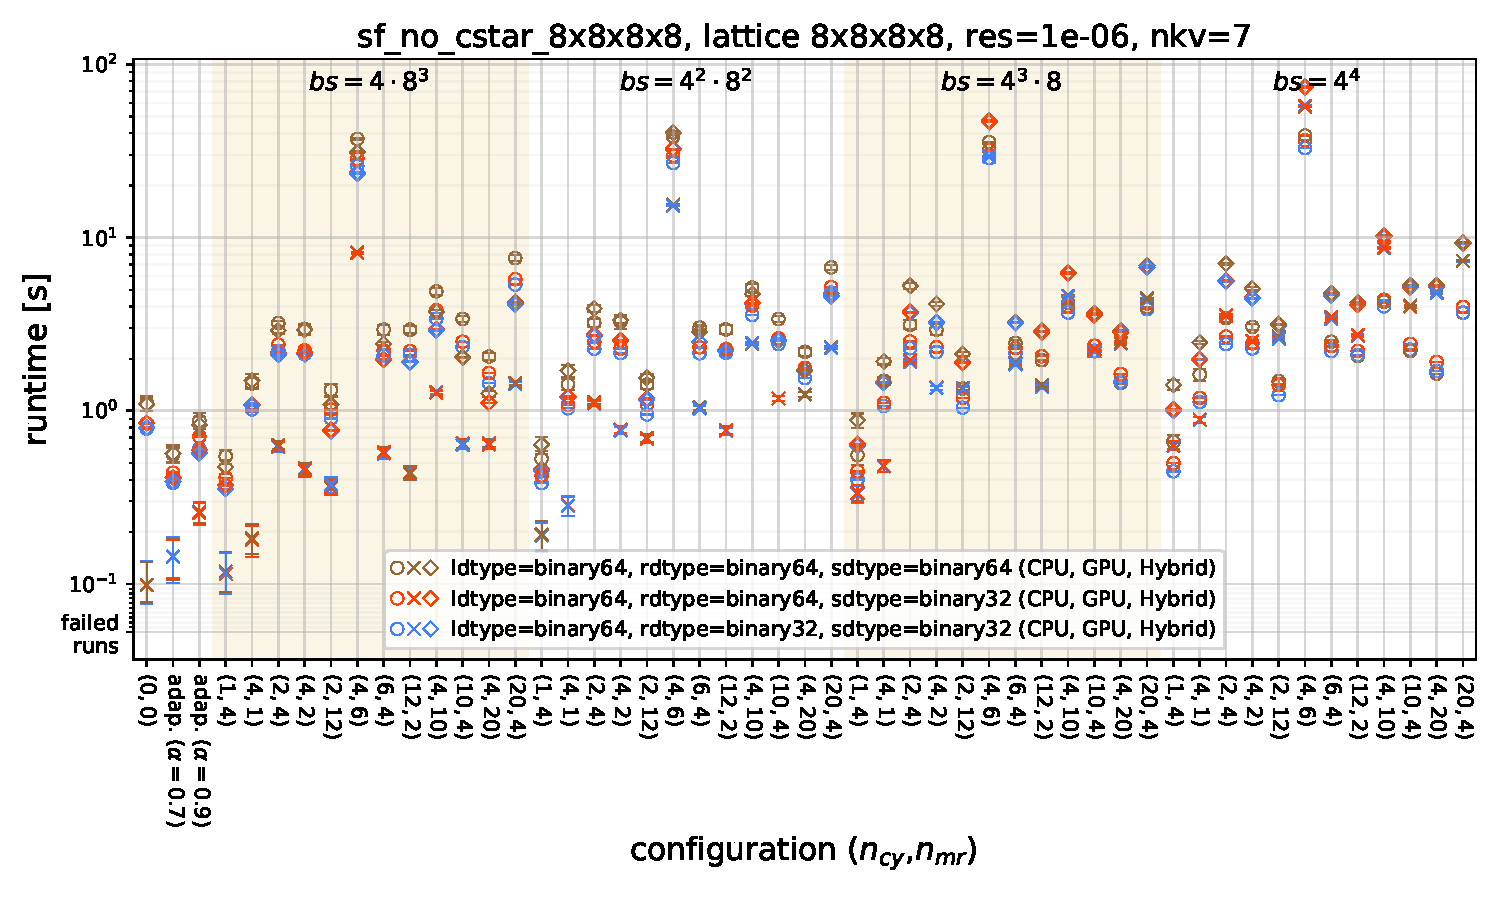
\includegraphics[width=1.0\textwidth]{plots/sap_gcr_sf_no_cstar_8x8x8x8_lattice_8x8x8x8_res=1e-06_nkv=7}
    \caption{Time measurements for the \code{SAP\_GCR} kernel on different matrices and configurations. The measurements where conducted on an AMD EPYC 7742 CPU @ 2.25GHz with 512 GB memory and an NVIDIA A100 (via SXM4) GPU with 40 GB memory.}
    \label{fig:sap_gcr0}
    \label{fig:sap_gcr_start}
    \label{fig:sap_gcr_sf_8x8x8x8}
\end{figure}

\begin{figure}[h]
    \centering
    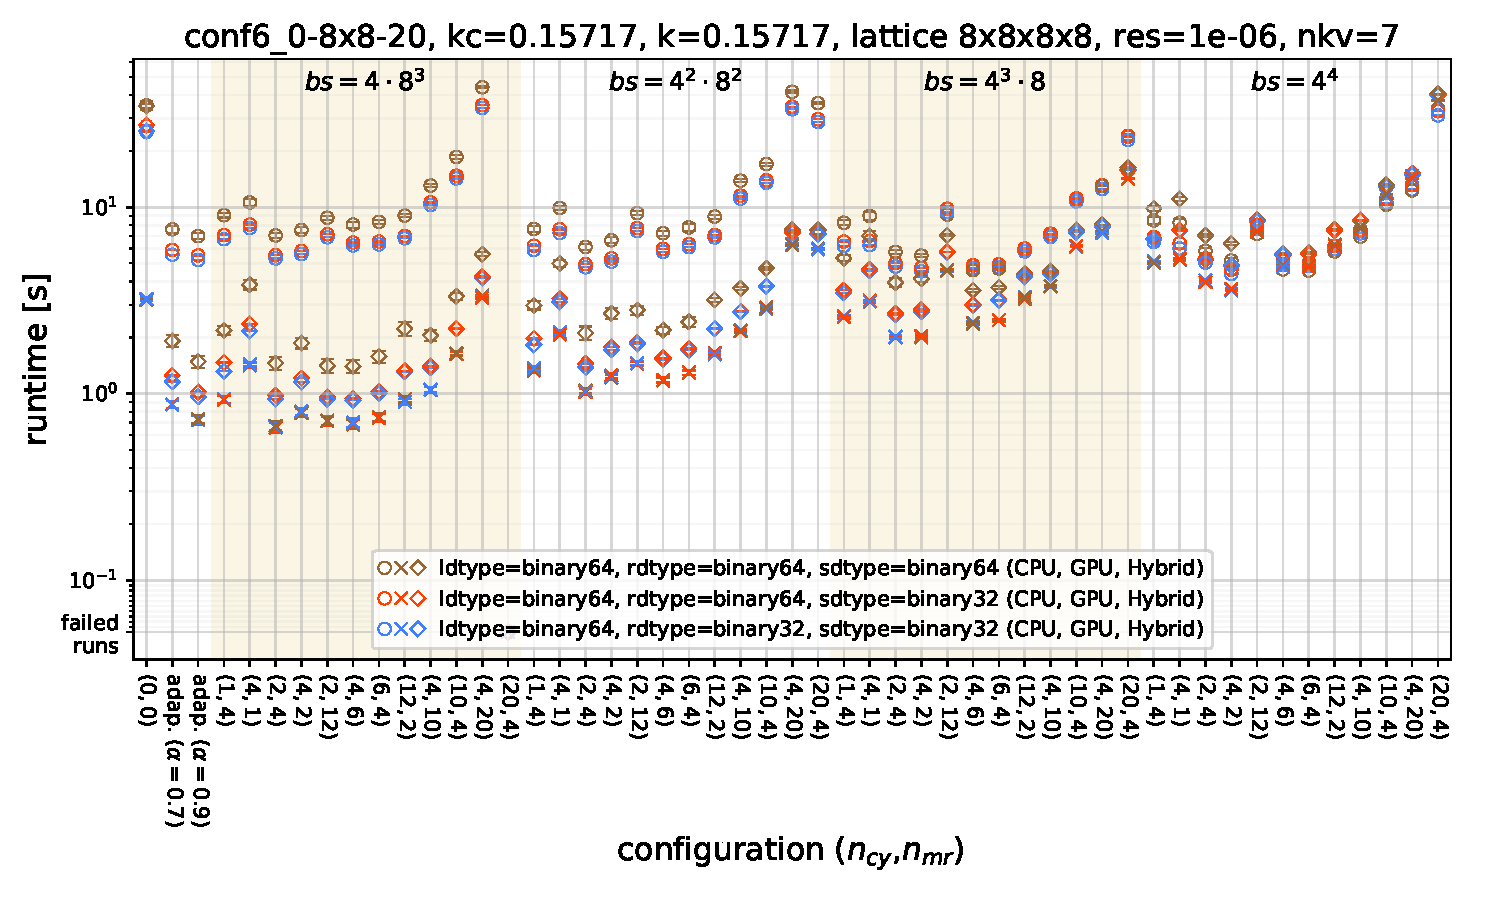
\includegraphics[width=1.0\textwidth]{plots/sap_gcr_conf6_0-8x8-20_kc=0.15717_k=0.15717_lattice_8x8x8x8_res=1e-06_nkv=7}
    \caption{Time measurements for the \code{SAP\_GCR} kernel on different matrices and configurations. The measurements where conducted on an AMD EPYC 7742 CPU @ 2.25GHz with 512 GB memory and an NVIDIA A100 (via SXM4) GPU with 40 GB memory.}
    \label{fig:sap_gcr1}
    \label{fig:sap_gcr_conf6_0-8x8-20_0.15717}
\end{figure}

\begin{figure}[h]
    \centering
    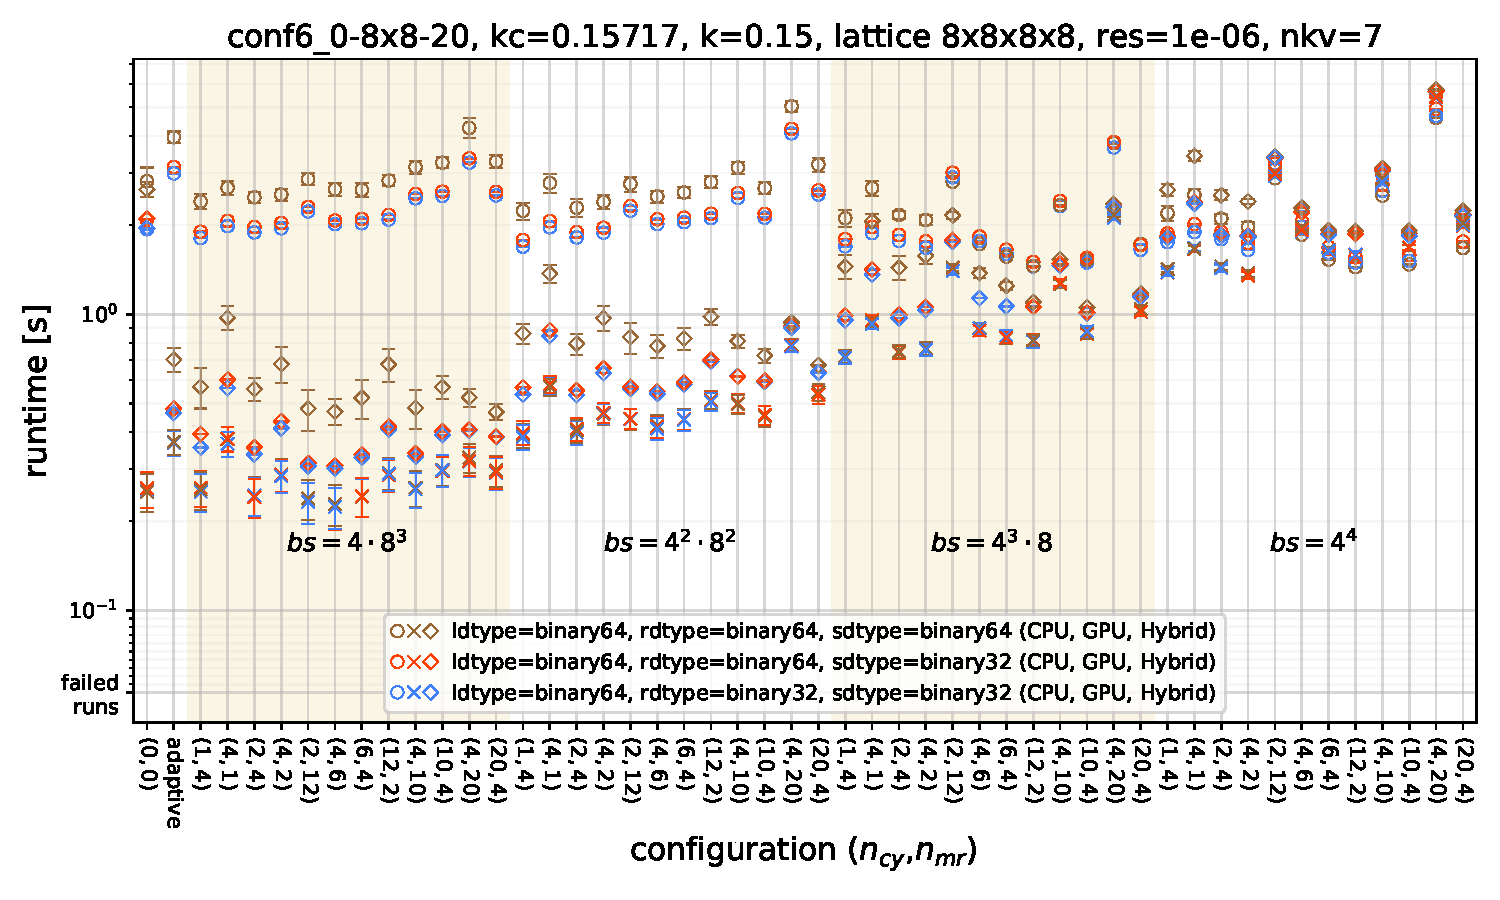
\includegraphics[width=1.0\textwidth]{plots/sap_gcr_conf6_0-8x8-20_kc=0.15717_k=0.15_lattice_8x8x8x8_res=1e-06_nkv=7}
    \caption{Time measurements for the \code{SAP\_GCR} kernel on different matrices and configurations. The measurements where conducted on an AMD EPYC 7742 CPU @ 2.25GHz with 512 GB memory and an NVIDIA A100 (via SXM4) GPU with 40 GB memory.}
    \label{fig:sap_gcr2}
    \label{fig:sap_gcr_conf6_0-8x8-20_0.15}
\end{figure}

\begin{figure}[h]
    \centering
    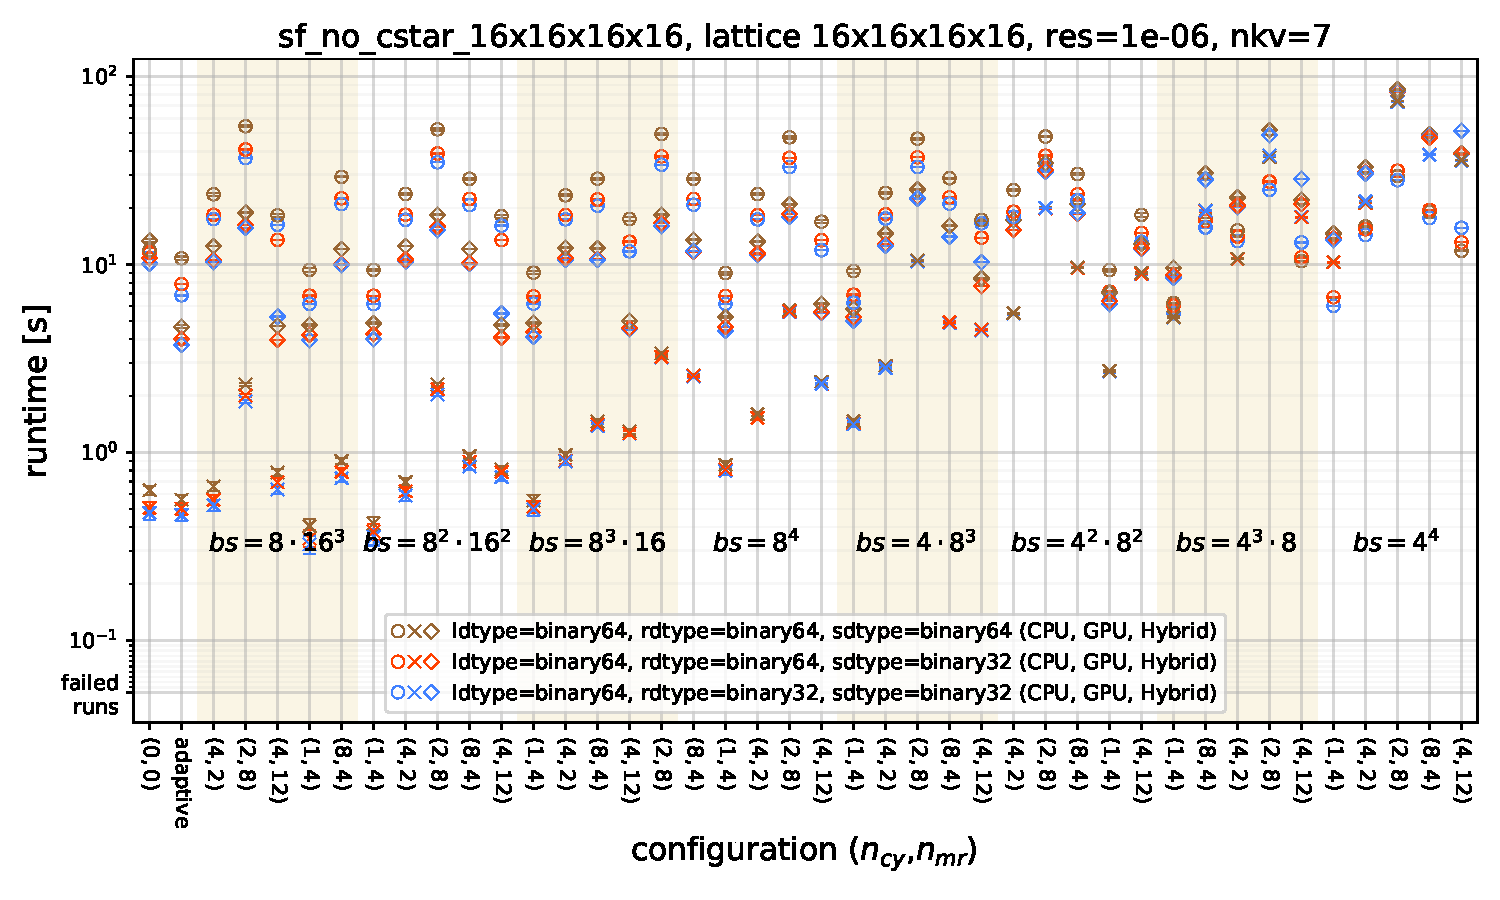
\includegraphics[width=1.0\textwidth]{plots/sap_gcr_sf_no_cstar_16x16x16x16_lattice_16x16x16x16_res=1e-06_nkv=7}
    \caption{Time measurements for the \code{SAP\_GCR} kernel on different matrices and configurations. The measurements where conducted on an AMD EPYC 7742 CPU @ 2.25GHz with 512 GB memory and an NVIDIA A100 (via SXM4) GPU with 40 GB memory.}
    \label{fig:sap_gcr3}
    \label{fig:sap_gcr_sf_16x16x16x16}
\end{figure}

\begin{figure}[h]
    \centering
    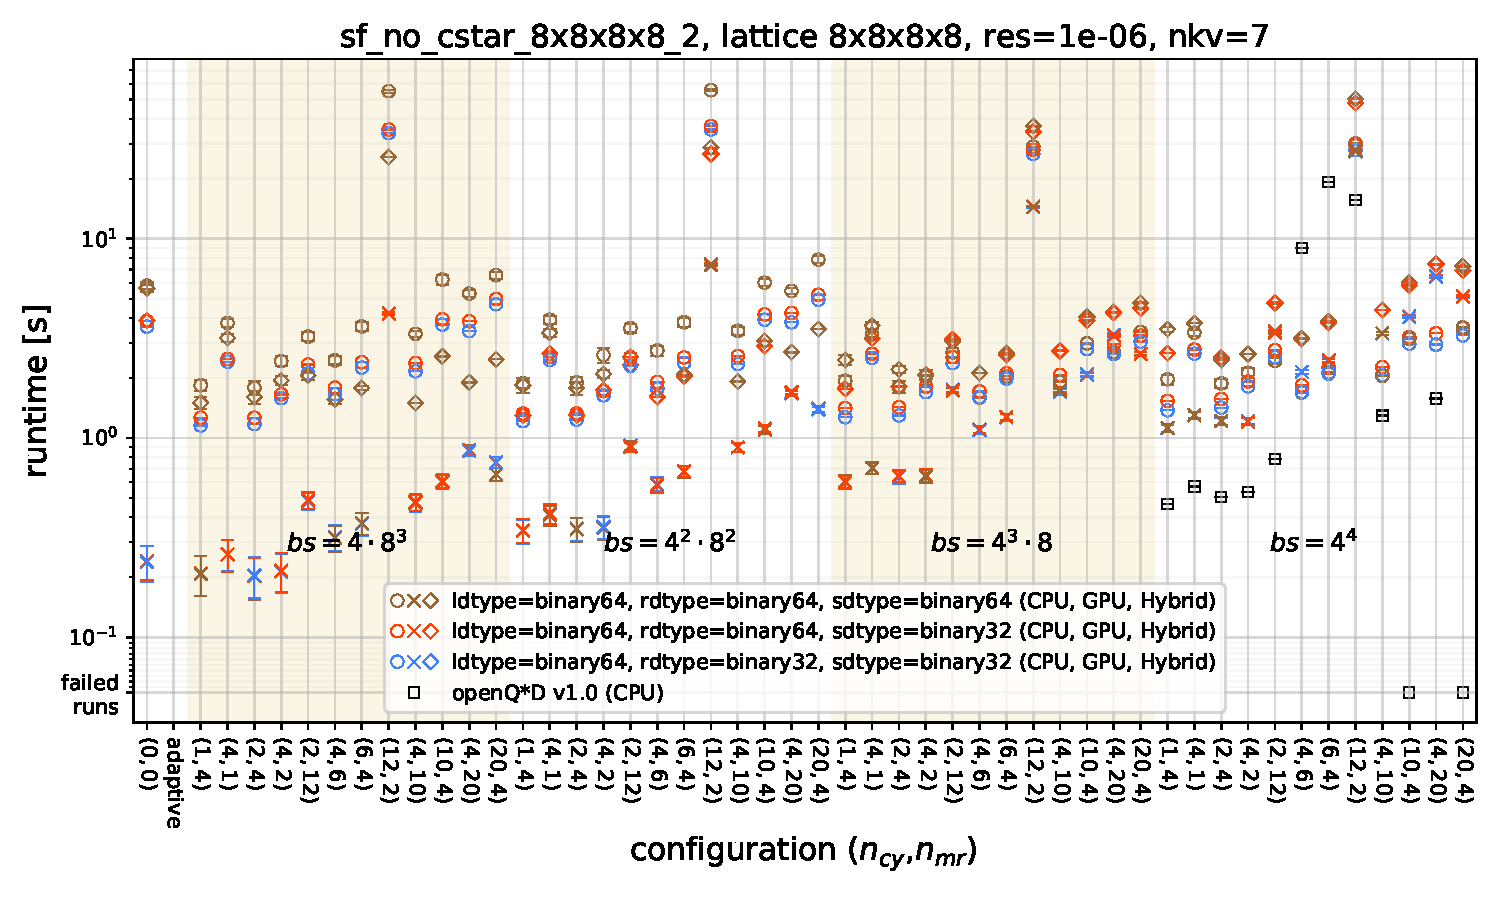
\includegraphics[width=1.0\textwidth]{plots/sap_gcr_sf_no_cstar_8x8x8x8_2_lattice_8x8x8x8_res=1e-06_nkv=7}
    \caption{Time measurements for the \code{SAP\_GCR} kernel on different matrices and configurations. The measurements where conducted on an Intel(R) 6130 @ 2.10GHz with 1.5 TB memory and an NVIDIA V100 (via PCIe) GPU with 16 GB memory.}
    \label{fig:sap_gcr4}
    \label{fig:sap_gcr_end}
    \label{fig:sap_gcr_sf_8x8x8x8_2}
\end{figure}

\subsubsection{Discussion of figures \ref{fig:sap_gcr_start} - \ref{fig:sap_gcr_end}}

An apparent trend visible in the whole plot series is that the pure-GPU variants are most efficient when the block size is large (the number of blocks is small). The pure-CPU variants behave different - the block size has less influence on the run-time. In general, the pure-GPU variants are faster than the pure-CPU ones. This comes from the fact that they take advantage of concurrency. The hybrid-variants are as expected in-between them, behaving similarly to the pure-GPU ones.

As further general observation, the power of the \acrshort{sapgcr} solver is only fully unfolded if the condition number of the operator is large; the plots of \code{sf\_no\_cstar\_8x8x8x8}, \code{sf\_no\_cstar\_8x8x8x8\_2} and \code{sf\_no\_cstar\_16x16x16x16} (figures \ref{fig:sap_gcr_sf_8x8x8x8}, \ref{fig:sap_gcr_sf_8x8x8x8_2} and \ref{fig:sap_gcr_sf_16x16x16x16}) show no significant performance improvement of the SAP-preconditioning compared to a pure GCR solver without preconditioning \footnote{The runs with configuration $(n_{cy}, n_{mr}) = (0,0)$}, whereas the runs on \code{conf6\_0-8x8-2} do (figures \ref{fig:sap_gcr_conf6_0-8x8-20_0.15717} and \ref{fig:sap_gcr_conf6_0-8x8-20_0.15}).

An analysis of the different datatypes shows that the general trend is the lower the involved datatypes are in bit-length, the faster the solution is obtained, which makes sense in memory-bound problems. The setups with \gls{binary32} in reduction variables (\code{rdtype}) and as "small" datatype (\code{sdtype}) appear to be the most efficient. On the CPU they display on average a speedup compared to the case where only \gls{binary64} was used of $S = 1.246$. However, of the given datatype setups one should choose the one where the datatype of reduction variables (\code{rdtype}) is set to \gls{binary64} preventing over- or underflows. This was already discussed in section \ref{sec:simulating_cgne} for the \acrshort{cgne}-solver.

Looking at the fist plot, figure \ref{fig:sap_gcr_sf_8x8x8x8}, as expected the preconditioning gives no significant improvement; on the CPU only \num{4} setups were faster than the one without preconditioning, on the GPU even none of the preconditioning setups beats the trivial case. Of all the CPU cases that were faster than the trivial case, all had the same configuration $(n_{cy}, n_{mr}) = (1,4)$, but different block sizes. This shows that if the operator is well-conditioned, too much preconditioning worsens the performance. $(n_{cy}, n_{mr}) = (1,4)$ is the configuration with the least amount of preconditioning. The CPU run-time shows a strong dependence on the configuration; there are even certain configurations (for example $(n_{cy}, n_{mr}) = (4,6)$) that are more than \num{40} times slower than the no preconditioning case. A wrong choice of configuration parameters can thus lead to a significant performance decrease, whatever "wrong" means exactly in this context. However, the plots show that performance of the algorithm is very sensitive to the choice of these parameters. The adaptive variant should here come to the rescue.

The operator \code{sf\_no\_cstar\_16x16x16x16} has a very similar behaviour as \code{sf\_no\_cstar\_8x8x8x8}, because it is well-conditioned as well. The very same configurations give speedup compared to the case without preconditioning, this time both the CPU and GPU variants improved. The claim that the pure-GPU variant slows down with smaller block sizes is even more visible in this plot, since there are \num{8} block sizes to work on. Looking at the behaviour within a certain constant block size, the algorithm seems to be very sensitive to changes in the configuration. As an example block size $bs= 8^2 \cdot 16^2$, one would expect the run-time to either increase or decrease with respect to the amount of preconditioning. The actual results show a more complex dependence with an exceptional case at $(n_{cy}, n_{mr}) = (2,8)$. That exceptional case can be seen with all block sizes and on the CPU, GPU as well as in the hybrid case. The plot of \code{sf\_no\_cstar\_8x8x8x8} features such an exceptional case as well at $(n_{cy}, n_{mr}) = (4,6)$. However, with both matrices any preconditioning makes the run-time worse, they might not be very representative.

Continuing to the matrix \code{conf6\_0-8x8-2} where the condition number depends on how close the $k = 0.15$ parameter is at its critical value $k_c = 0.15717$. This is the regime where the preconditioning shows benefits. For the pure-CPU cases, we see no strong dependence on the amount of preconditioning, but on the block size. Small block sizes seem to be beneficial, whereas the pure-GPU variant prefers large block sizes. Similar to the above analysis, the good condition number again give not much speedup gain, when comparing the preconditioned cases with the trivial case.

Using the same matrix as above, but at the critical point $k=k_c$, we are in the regime where the \acrshort{sapgcr} algorithm shows its true potential; nearly all cases performed better than the trivial case without any preconditioning. The pure-GPU cases behave as usual - large block sizes are better. This time even the pure-CPU shows a dependence on the block size. Although, it's a weak dependence, but with smaller block sizes the CPU seems to perform slightly better (on contrary to the GPU). The hybrid cases - as usual in-between - are closer to the pure-GPU ones, because despite being hybrid most of the work is done on the GPU. The pattern within a certain block size is repeating and the best amount of preconditioning seems to be at $(n_{cy}, n_{mr}) = (4,6)$.

Last but not least, the second matrix from openQxD \code{sf\_no\_cstar\_8x8x8x8\_2} (figure \ref{fig:sap_gcr_sf_8x8x8x8_2}) shows similar patterns as the matrix first matrix with the same configuration. The measurement was repeated in order to check whether there is a visible pattern common to both matrices. Unfortunately this is not the case. Although it is noticable that there is also an exceptional configuration that took disproportionally longer than the others at $(n_{cy}, n_{mr}) = (12,2)$. More importantly it is not the same configuration, making it hard to determine the best set of parameters beforehand and at the same time maintaining an perfect amount of preconditioning for all invocations of the solver.

%The discussion is just a more extreme version of the previous paragraph. Within all block sizes, one can see the same pattern repeating. It seems that the configurations involving large amounts of preconditioning (large \code{ncy}, \code{nmr}) perform worse.

\subsubsection{Conclusion}

In general two different patterns can be observed in the above plot series. Either the matrix is bad conditioned and one can see that most of the preconditioned runs perform better than no preconditioning. Or the matrix is good conditioned and the preconditioned cases perform worse. In both cases the pattern within a block size repeats in other blocks sizes, but shifted. We see two types of patterns. For bad conditioned systems the pattern shows that the ideal case is at some point in the middle. On the other hand for well-conditioned system, the pattern seems random, but a increase of run-time with more preconditioning (higher values of $n_{cy}$ and $n_{mr}$) can be seen. Since the systems are already well conditioned, too much preconditioning can worsen the run-time.


Since the algorithm is applied to many different Dirac-operators among evolving \acrshort{hmc}-trajectories - some well-conditioned, some ill-conditioned - it can be hard or even impossible to choose a set of parameters suitable for all cases. Specially, it is unavoidable to accidentially make a choice that falls on a configuration with exceptional long convergence time for a certain Dirac-operator within the long running HMC-simulation. It is therefore advisable to have the possibility to change the parameters during an active run or a configuration that adapts. This motivates the following proposal.

\begin{proposal}{Adaptive choice of parameters in \acrshort{sapgcr}}{adaptive}

Since the choice of parameters in the \acrshort{sapgcr} kernel seems non-trivial, we propose a adaptive variant of this algorithm. The parameters $n_{cy}$, $n_{mr}$ where chosen automatically in every iteration anew, the block size was chosen to be the largest possible. The adaptive choice was done as follows: If - after a Schwarz-cycle - the norm of the residual is not lower than the residual norm before the cycle, then the preconditioning phase is exited. Thus, at least one Schwarz-cycle is performed. A similar, but slightly more complicated strategy is applied to determine the number of MR-steps. There are \num{3} exit conditions for the MR-solver:

\begin{enumerate}[label={\arabic*)}]
  \item If - after at least \num{4} MR-steps - the norm of the residual on the block is larger than $\alpha = 0.9$\footnote{Ironically, the choice for the value of $\alpha \in (0, 1]$ is again non-trivial. Small values cause less preconditioning whereas values close to \num{1} will end up in more or even the maximal amount of MR-steps. But since we want to optimise for ill-conditioned systems and the penalty for well-conditioned systems is not too hard, it is advisable to choose $\alpha$ large, such as $\alpha = 0.9$} times the previous residual norm, the MR-solver exits and the application continues processing the next block.
  \item If the norm of the blocked residual became larger than the previous residual norm, exit immediately, even if only one MR-step is executed.
  \item If the norm of the blocked residual is smaller than the tolerance\footnote{This is the tolerance calculated in the GCR solver divided by the number of blocks, $tol = res*\norm{\eta}/n_b$, where \code{res} is the desired relative residual given as configuration option (see table \ref{tab:sap_gcr_settings}), $\eta = \vec{b}$ is the source vector and $n_b$ is the number of blocks.}, also exit immediately.
\end{enumerate}

So, every block is treated differently in every cycle. A maximum of \num{20} Schwarz-cycles and \num{20} MR-steps on each block would be performed if the above exit conditions will never kick in. The third exit condition above makes sure to not overshoot the mark if the algorithm performs a lot of Schwarz-cycles and MR-steps. Namely, if the problem is already solved while in the preconditioning phase. This can happen if the operator is very well-conditioned or in the very last GCR-step before converging to the desired relative residual. Therefore the adaptive version tries to find the optimal configuration for every iteration of the \acrshort{gcr}-solver, for every Schwarz-cycle and for every block separately. By empirical observation of the results, the adaptive variant usually performs nearly maximal amounts of preconditioning in the first few GCR-steps, then rapidly decreases after some steps to a much less amounts and finally saturating to the minimal amount that stays until convergence.

The results on how this adaptive variant competes with static configurations can be seen in figures \ref{fig:sap_gcr_start} - \ref{fig:sap_gcr_end}. The adaptive runs are indicated with configuration $adap.$ with two different values of $\alpha$. Although the adaptive variant of the algorithm is not the fastest among all configurations, the plots show that it is certainly the most versatile one. It is though to be chosen if the condition of the operator is not known beforehand and might even change drastically within a long running simulation.

\end{proposal}

In openQxD, every rank has its own local lattice to process. The solver algorithms are implemented in a parallel manner, such that the solver is called on all ranks simultaneously. The simulation problem was chosen to be such that the task of one rank was compared on one single core of the CPU and on one single GPU (with all its parallelizability). It is therefore not surprising that most of the time, the GPU solved the problem much faster than the CPU. Keeping this in mind, it is natural to associate a larger local lattice to the available GPUs in the system (maybe 4-8 times larger, depending on the available memory) and let them participate to the solution of the full problem just as they were additional ranks (compare proposal \ref{pp:gpu_implementation1}).

\section{Deflated SAP preconditioned GCR algorithm}

The low modes of the Dirac operator condensate TODO.

Small quark masses corresponding to real physics are believed to be the cause for the spontaneously breaking of chiral symmetry in lattice QCD \cite{banks1980}. Numerical lattice QCD has the problem that with large lattice volumes and small quark masses simulation techniques become inefficient in the \df{chiral regime} (where chiral symmetry is spontaneously broken), because the Dirac operators gets more and more ill-conditioned. Thus, the presence of low eigenvalues is a source of difficulty \cite{giusti2003}. According to the Bank-Casher relation \cite{banks1980}, this is because the number of eigenvalues of $D$ below a fixed value grows with $O(V)$, where $V$ is the total 4D lattice volume. On the other hand, the computational effort scales even worse with $O(V^2)$ \cite{luscher2007}. This behaviour goes under the name of \df{$V^2$-problem}.

A solving algorithm that has a flat scaling with respect to the quark masses can therefore lead to large speedups specially in that regime. By deflating the Dirac operator, it is possible to separate eigenmodes with very small eigenvalues from the others. Thus the space needs to be split in low and high modes without actually calculating the modes, else the problem would be solved already.

\subsection{Deflation}

\begin{theorem}[Deflation]

\label{thm:deflation}

Let $A$ be a linear, invertible operator acting on a vector space $\Lambda$, $\vec{b} \in \Lambda$ an arbitrary vector and $P_L$ a projector\footnote{$P_L$ does not have to be orthogonal or Hermitian.} acting on $\Lambda$. Also, define the linear operator $P_R$ such that $P_L A = A P_R$\footnote{Such a linear operator $P_R$ always exists - just set $P_R \coloneqq A^{-1} P_L A$, since $A$ is invertible.}. Consider 

\begin{align}
    \vec{x}^{\star} \coloneqq P_R \vec{x}^{\star}_1 + (1-P_R) \vec{x}^{\star}_2, \label{eq:def_projection}
\end{align}

with $\vec{x}^{\star}_1$ and $\vec{x}^{\star}_2$ being solutions to the "smaller" (projected) systems

\begin{align*}
    P_L A \vec{x}_1 &= P_L \vec{b}
    & &\text{and} &
    (1-P_L)A \vec{x}_2 &= (1-P_L)\vec{b}
\end{align*}

respectively. Then 

\begin{enumerate}[label={\arabic*)}]
  \item $P_R$ is a projector,
  \item $\vec{x}^{\star}$ is the unique solution to $A\vec{x} = \vec{b}$.
\end{enumerate}

\end{theorem}

\begin{proof}

Using that $P_L^2 = P_L$ is a projector and the defining relation $P_L A = A P_R$,

\begin{align*}
    P_R^2 &= (A^{-1} P_L A)^2 \\
    &= A^{-1} P_L^2 A \\
    &= A^{-1} P_L A \\
    &= P_R.
\end{align*}

By direct calculation,

\begin{align*}
    A \vec{x}^{\star} &= A P_R \vec{x}^{\star}_1 + A (1-P_R) \vec{x}^{\star}_2 \\
    &= P_L A \vec{x}^{\star}_1 + (1-P_L) A \vec{x}^{\star}_2 \\
    &= P_L \vec{b} + (1-P_L)\vec{b} \\
    &= \vec{b}.
\end{align*}

Since $A$ is invertible $\vec{x}^{\star}$ is unique, although $\vec{x}^{\star}_1$ and $\vec{x}^{\star}_2$ may not be unique, their projections are.

\end{proof}

\begin{remark}
If we find clever subspaces in which the projectors $P_L$ and $P_R$ project without involving $A^{-1}$, we can solve $A\vec{x} = \vec{b}$ by solving the \num{2} smaller systems of equations and then projecting the solutions using $P_R$.
\end{remark}

\begin{remark}
Notice that $P_L A$ as well as $(1-P_L)A$ are not invertible. There are infinitely many solutions $\vec{x}^{\star}_1$ and $\vec{x}^{\star}_2$\footnotemark. Nonetheless the solution vector $\vec{x}^{\star}$ is still unique after the projection in equation \eqref{eq:def_projection}, because $P_R$ removes all ambiguity from the vector.
\end{remark}

\footnotetext{Let $P$ be a linear projector (not the identity-operator) and $A$ an invertible linear operator. The system of interest is $PA\vec{x} = P\vec{b}$. There exists at least one solution to this, namely the unique solution to $A\vec{x} = \vec{b}$. Since $PA$ is not invertible, the only two possibilities are zero or infinite solutions and it can't be zero solutions.}

\begin{remark}
Comparing deflation to left preconditioning, the difference is that in deflation $P_L$ is a projector and $P_L A$ has condition number infinite whereas in case of preconditioning $P_L $ is invertible (a good approximation of $A^{-1}$) and the condition number of $P_L A$ is expected to be smaller than the one of $A$.
\end{remark}

\begin{remark}
If $A$ is positive definite, $P_L A \vec{x} = P_L \vec{b}$ is positive semidefinite, has infinite solutions and condition number infinite. Fortunately such a system can be solved as long as the right-hand side is consistent, meaning that there exists a $\vec{x}$ solving $A \vec{x} = \vec{b}$ \cite{kaasschieter1988}.
\end{remark}

Therefore it makes sense to define the relevant quantity.

\begin{definition}[Effective condition number]

The \df{effective condition number} of a matrix $A$ is the ratio between the largest and smallest eigenvalue with positive magnitude

\begin{align*}
  \kappa_{eff}(A) &\coloneqq \frac{\abs{\lambda_{max}}}{\abs{\lambda_{pmin}}} \\
  \abs{\lambda_{max}} &= \max \abs{\sigma(A)} \\
  \abs{\lambda_{pmin}} &= \min \{ \abs{\lambda} \, \bigm\lvert \, \lambda \in \sigma(A), \abs{\lambda} > 0 \}.
\end{align*}

\end{definition}

\begin{remark}
The condition number and the effective condition number are equal if the matrix $A$ is invertible.
\end{remark}

\begin{corollary}

\label{cor:deflation}

Let $A$, $\Lambda$ and $\vec{b}$ be as in theorem \ref{thm:deflation}. Furthermore let $\{ \vec{\omega}_i \}_{i=1}^N$ be a orthonormal basis of a linear subspace $\Omega \subset \Lambda$, called the \df{deflation subspace} and let the restriction of $A$ to $\Omega$, $\widetilde{A} \coloneqq \restr{A}{\Omega}$ called the \df{little operator}, be invertible. Define $P_L$ by its action on an arbitrary vector $\vec{x} \in \Lambda$ as

\begin{align*}
    P_L \vec{x} &\coloneqq \vec{x} - \sum_{i,j=1}^N A \vec{\omega}_i (\widetilde{A}^{-1})_{ij} \langle \vec{\omega}_j, \vec{x} \rangle
    %P_R \vec{y} &= \vec{y} - \sum_{i,j=1}^N \vec{\omega}_i (\widetilde{A}^{-1})_{ij} \langle \vec{\omega}_j, A \vec{y} \rangle,
\end{align*}

and let $\vec{x}^{\star}_1$ be one of the (infinite) solutions to the \df{deflated system} $\hat{A} \vec{x}_1 = P_L \vec{b}$, where $\hat{A} \coloneqq P_L A$ is called the \df{deflated operator}. Consider

\begin{align}
    \vec{x}^{\star} \coloneqq P_R \vec{x}^{\star}_1 + \sum_{i,j=1}^N \vec{\omega}_i (\widetilde{A}^{-1})_{ij} \langle \vec{\omega}_j, \vec{b} \rangle, \label{eq:defl_soln}
\end{align}

with $P_R$ satisfying $P_L A = A P_R$. Then $\vec{x}^{\star}$ is the unique solution to the linear system of equations $A \vec{x} = \vec{b}$.

\end{corollary}

\begin{proof}

Lets first show that $P_L^2 = P_L$ is a projector,

\begin{align*}
    P_L^2 \vec{x} &= P_L \left( \vec{x} - \sum_{i,j=1}^N A \vec{\omega}_i (\widetilde{A}^{-1})_{ij} \langle \vec{\omega}_j, \vec{x} \rangle \right) \\
    &= \vec{x} - 2 \sum_{i,j=1}^N A \vec{\omega}_i (\widetilde{A}^{-1})_{ij} \langle \vec{\omega}_j, \vec{x} \rangle + \sum_{i,j=1}^N A \vec{\omega}_i (\widetilde{A}^{-1})_{ij} \sum_{k,l=1}^N \langle \vec{\omega}_j, A \vec{\omega}_k \rangle (\widetilde{A}^{-1})_{kl} \langle \vec{\omega}_l, \vec{x} \rangle \\
    &= \vec{x} - 2 \sum_{i,j=1}^N A \vec{\omega}_i (\widetilde{A}^{-1})_{ij} \langle \vec{\omega}_j, \vec{x} \rangle + \sum_{i,j,l=1}^N A \vec{\omega}_i (\widetilde{A}^{-1})_{ij} \langle \vec{\omega}_l, \vec{x} \rangle \underbrace{\sum_{k=1}^N \underbrace{\langle \vec{\omega}_j, A \vec{\omega}_k \rangle}_{= \widetilde{A}_{jk}} (\widetilde{A}^{-1})_{kl} }_{= \delta_{jl}} \\
    &= \vec{x} - 2 \sum_{i,j=1}^N A \vec{\omega}_i (\widetilde{A}^{-1})_{ij} \langle \vec{\omega}_j, \vec{x} \rangle + \sum_{i,j=1}^N A \vec{\omega}_i (\widetilde{A}^{-1})_{ij} \langle \vec{\omega}_j, \vec{x} \rangle \\
    &= \vec{x} - \sum_{i,j=1}^N A \vec{\omega}_i (\widetilde{A}^{-1})_{ij} \langle \vec{\omega}_j, \vec{x} \rangle \\
    &= P_L \vec{x}.
\end{align*}

Now lets show that the second term in equation \eqref{eq:defl_soln} is equal to $(1-P_R)\vec{x}^{\star}_2$ where $\vec{x}^{\star}_2$ solves the projected system $(1-P_L)A \vec{x}_2 = (1-P_L) \vec{b}$.

\begin{align*}
    (1-P_R)\vec{x}^{\star}_2 &= A^{-1} (1-P_L) A \vec{x}^{\star}_2 \\
    &= A^{-1} (1-P_L) \vec{b} \\
    &= A^{-1} \sum_{i,j=1}^N A \vec{\omega}_i (\widetilde{A}^{-1})_{ij} \langle \vec{\omega}_j, \vec{b} \rangle \\
    &= \sum_{i,j=1}^N \vec{\omega}_i (\widetilde{A}^{-1})_{ij} \langle \vec{\omega}_j, \vec{b} \rangle 
\end{align*}

which corresponds to the second term of $\vec{x}^{\star}$ in equation \eqref{eq:defl_soln}, therefore $\vec{x}^{\star} \coloneqq P_R \vec{x}^{\star}_1 + (1-P_R) \vec{x}^{\star}_2$. By application of theorem \ref{thm:deflation}, $\vec{x}^{\star}$ is the unique solution to $A\vec{x} = \vec{b}$.

\end{proof}

\begin{remark}
From $P_L$ in corollary \ref{cor:deflation}, the action of $P_R$ on a arbitrary vector $\vec{x}$ can be determined using the defining relation of $P_R$ as

\begin{align*}
    P_R\vec{x} &= A^{-1} P_L A \vec{x} \\ 
    &= \vec{x} - \sum_{i,j=1}^N \vec{\omega}_i (\widetilde{A}^{-1})_{ij} \langle \vec{\omega}_j, A \vec{x} \rangle.
\end{align*}
\end{remark}

\begin{remark}
An application of $P_L$ to an arbitrary vector $\vec{x}$ involves solving the \df{little system} $\widetilde{A} \vec{\beta} = \vec{\alpha}$ on $\Omega$ for a given $\vec{\alpha} \in \Omega$. To see this, lets look at the $k$-th component of $P_L \vec{x}$

\begin{align*}
    (P_L\vec{x})_k &\coloneqq x_k - \sum_{i,j=1}^N (A\vec{\omega}_i)_k (\widetilde{A}^{-1})_{ij} \langle \vec{\omega}_j, \vec{x} \rangle.
\end{align*}

Define the vector

\begin{align*}
    \vec{\alpha}_{\vec{x}} &\coloneqq
    \begin{pmatrix}
        \langle \vec{\omega}_1, \vec{x} \rangle \\
        \langle \vec{\omega}_2, \vec{x} \rangle \\
        \vdots \\
        \langle \vec{\omega}_N, \vec{x} \rangle
    \end{pmatrix} = \begin{pmatrix}
        (\vec{\omega}_1)_1 & \hdots & (\vec{\omega}_1)_N \\
        (\vec{\omega}_2)_1 & \hdots & (\vec{\omega}_2)_N \\
        \vdots & \ddots & \vdots \\
        (\vec{\omega}_N)_1 & \hdots & (\vec{\omega}_N)_N
    \end{pmatrix} \begin{pmatrix}
        x_1 \\
        x_2 \\
        \vdots \\
        x_N
    \end{pmatrix}.
\end{align*}

Then

\begin{align*}
    (P_L\vec{x})_k &= x_k - \sum_{i=1}^N (A\vec{\omega}_i)_k ( \textcolor{cyellow}{\widetilde{A}^{-1} \vec{\alpha}_{\vec{x}}} )_i \\
    &= x_k - \sum_{i=1}^N (A\vec{\omega}_i)_k \textcolor{cyellow}{\vec{\beta}}_i.
\end{align*}

By similar analysis, an application of $P_R$ has the same cost with one additional application of $A$. For an efficient implementation of $P_L$ and $P_R$, the $2N$ vectors $\{A\vec{\omega}_i\}_{i=1}^N$ and $\{\vec{\omega}_i\}_{i=1}^N$ have to be kept in system memory.

\end{remark}

\begin{remark}

% TODO: work through this again -> local coherence

Assuming that the condition number of $A$ is high and the \df{spectrum} of $A$, $\sigma(A)$, is separable in a way such that

\begin{align}
    \sigma(A) &= \sigma_l(A) \cup \sigma_h(A)
    & &\text{with} &
    \max\limits_{\lambda \in \sigma_l(A)} \abs{\lambda} &\ll \min\limits_{\lambda \in \sigma_h(A)} \abs{\lambda}. \label{eq:separable}
\end{align}

The subscripts stand for "low" and "high", corresponding to the low and high modes of the operator $A$. So, the property in equation \eqref{eq:separable} states that the bulk of the low eigenvalues are somehow clustered\footnote{The high eigenmodes may not be clustered, but still separated from the low ones.}. Consider the linear sub-spaces $\Omega_l, \Omega_h \subset \Lambda$ such that the low and high eigenvectors corresponding to the low and high eigenvalues of $A$ are contained in $\Omega_l$ and $\Omega_h$ respectively. Then the condition number of $A$ restricted to the low modes is much smaller than the condition number of $A$. Therefore, if we are able to find a orthonormal basis $\{\vec{\omega}_i\}_{i=0}^N$ of the subspace $\Omega_l$ containing the bulk of the low eigenmodes of $A$, we can apply deflation from corollary \ref{cor:deflation} to solve the little equation that has a significantly smaller condition number than $A$. Then find one of the infinite solutions to the deflated system and construct a solution of the full system.

% TODO: why is it easy to solve the deflated system?
% TODO: define condition number \kappa(A) = ... somewhere.

\end{remark}

\begin{lemma}
\label{lem:condition_number}

Let $A$, $\{\vec{\omega}_i\}_{i=1}^N \in \Omega$, $P_L$, $P_R$ be as in corollary \ref{cor:deflation} and assume that the spectrum of $A$ is separable \eqref{eq:separable}. Define the deflation subspace to be the subspace corresponding to the low eigenmodes, $\Omega \coloneqq \Omega_l$. Then $\kappa_{eff}(\hat{A}) \ll \kappa(A)$ and $\kappa(\tilde{A}) \ll \kappa(A)$.
\end{lemma}

\begin{proof}

Lets define the orthogonal projector $P^{\perp}$ to $\Omega^{\perp}$, the orthogonal complement of the deflation subspace $\Omega$,

\begin{align*}
    P^{\perp} \vec{x} \coloneqq \vec{x} - \sum_{i=1}^N \langle \vec{\omega}_i, \vec{x} \rangle \vec{\omega}_i.
\end{align*}

The deflated operator $\hat{A} \coloneqq P_L A$ acts on the orthogonal complement,

\begin{align*}
    \hat{A} P^{\perp} \vec{x} &= P_L A P^{\perp} \vec{x} \\
    &= P_L A \vec{x} - \sum_{k=1}^N P_L A \vec{\omega}_k \langle \vec{\omega}_k, \vec{x} \rangle \\
    &= A \vec{x} - \sum_{i,j=1}^N A \vec{\omega}_i (\widetilde{A}^{-1})_{ij} \langle \vec{\omega}_j, A \vec{x} \rangle - \sum_{k=1}^N A \vec{\omega}_k \langle \vec{\omega}_k, \vec{x} \rangle + \sum_{i,k=1}^N A \vec{\omega}_i \underbrace{ \sum_{j=1}^N (\widetilde{A}^{-1})_{ij} \underbrace{\langle \vec{\omega}_j, A \vec{\omega}_k \rangle}_{=\widetilde{A}_{jk}} }_{\delta_{ik}} \langle \vec{\omega}_k, \vec{x} \rangle \\
    &= A \vec{x} - \sum_{i,j=1}^N A \vec{\omega}_i (\widetilde{A}^{-1})_{ij} \langle \vec{\omega}_j, A \vec{x} \rangle - \sum_{k=1}^N A \vec{\omega}_k \langle \vec{\omega}_k, \vec{x} \rangle + \sum_{k=1}^N A \vec{\omega}_k \langle \vec{\omega}_k, \vec{x} \rangle \\
    &= A \vec{x} - \sum_{i,j=1}^N A \vec{\omega}_i (\widetilde{A}^{-1})_{ij} \langle \vec{\omega}_j, A \vec{x} \rangle \\
    &= P_L A \vec{x} \\
    &= \hat{A} \vec{x}.
\end{align*}

Define the \df{minimal and maximal eigenvalue} of $A$,

\begin{align*}
    \lambda_{pmin}(A) &\coloneqq \min\limits_{\lambda \in \sigma(A), \abs{\lambda} > 0} \abs{\lambda}
    & &\text{and} &
    \lambda_{max}(A) &\coloneqq \max\limits_{\lambda \in \sigma(A)} \abs{\lambda}.
\end{align*}

The condition number of $\hat{A}$ can now be upper bounded,

\begin{align*}
    \kappa_{eff}({\hat{A}}) = \frac{\abs{\lambda_{max}(\hat{A})}}{\abs{\lambda_{pmin}(\hat{A})}} \ll \frac{\abs{\lambda_{max}(A)}}{\abs{\lambda_{pmin}(\hat{A})}} \le \frac{\abs{\lambda_{max}(A)}}{\abs{\lambda_{min}(A)}} = \kappa({A}),
\end{align*}

where property \eqref{eq:separable} was used in the first inequality. Similar for the condition number of the little operator $\kappa({\tilde{A}})$ where we have $\sigma(\tilde{A}) = \sigma(\restr{A}{\Omega}) = \sigma_l$ which directly implies $\kappa(\tilde{A}) \ll \kappa(A)$.

\end{proof}

\begin{remark}
Lemma \ref{lem:condition_number} tells us that the deflated and the little system are significantly better conditioned than the full system and both are therefore solved in fewer iterations\footnote{Additionally the little system is much smaller in size than the full system, but the sparsity will not stay - it might even become dense. Also the precision up to which this system has to be solved in an application of the projector is usually a fraction of the desired precision to the full solution.}. But this holds only if we are able to find the subspace corresponding to the low eigenmodes $\Omega_l$ and if the low eigenvalues of the matrix are somehow isolated from the bulk of the eigenvalues. Equation \eqref{eq:separable} gives us a condition on $A$ for a efficient deflation.
\end{remark}

\begin{lemma}

$P_L$ as defined in corollary \ref{cor:deflation} is a projection to the orthogonal complement of $\Omega$, i.e. $\langle \vec{\omega}_k, P_L \vec{x} \rangle = 0$.

\end{lemma}

\begin{proof}

Let $\vec{x}$ be an arbitrary vector, and $k \in \{1, \dots, N\}$, then

\begin{align*}
    \langle \vec{\omega}_k, P_L \vec{x} \rangle &= \langle \vec{\omega}_k, \vec{x} \rangle - \sum_{i,j=1}^N \langle \vec{\omega}_k, A \vec{\omega}_i \rangle (\widetilde{A}^{-1})_{ij} \langle \vec{\omega}_j, \vec{x} \rangle \\
    &= \langle \vec{\omega}_k, \vec{x} \rangle - \sum_{j=1}^N \langle \vec{\omega}_j, \vec{x} \rangle \sum_{i=1}^N \widetilde{A}_{ki} (\widetilde{A}^{-1})_{ij} \\
    &= \langle \vec{\omega}_k, \vec{x} \rangle - \sum_{j=1}^N \langle \vec{\omega}_j, \vec{x} \rangle \delta_{kj} \\
    &= 0.
\end{align*}

\end{proof}

\subsection{Choosing the deflation subspace}

\label{sec:dfl_subspace}

Besides isolated low eigenmodes, the Dirac-operator should feature another property in order for deflation to be efficient. The computational cost to find an approximation of the low-mode deflation subspace should not be too high. It turns out that if the low eigenmodes of the Dirac-operator possess a certain property, only a few low eigenmodes are needed to construct a good approximation of the subspace of low eigenmodes $\Omega_l$. If the subspace of low eigenmodes is only approximated, the method is called \df{inexact deflation}.

\begin{comment}
\begin{definition}[Local coherence]

\label{def:local_coherence}

Let $\varepsilon > 0$, $M,N \in \mathbb{N}$ with $M \ll N$ and $\Lambda$ be the full lattice. Let $B \coloneqq \{\vec{\beta}_i\}_{i=1}^N$ and $C \coloneqq \{\vec{\gamma}_j\}_{j=1}^M$ with $\vec{\beta}_i,\vec{\gamma}_j \in \Lambda$ be two sets of fields. Furthermore define the projector $P_{\Gamma}$ to the subspace $\Gamma \coloneqq span(C)$ via its action onto an arbitrary vector $\vec{x} \in \Lambda$ as

\begin{align*}
    P_{\Gamma} \vec{x} \coloneqq \sum_{j=1}^M \langle \vec{\gamma}_j, \vec{x} \rangle \vec{\gamma}_j.
\end{align*}

The fields $B$ are \df{locally coherent} with the fields $C$ up to $\varepsilon$, if $\forall i \in \{1, \dots N\}$

\begin{align*}
    \norm{ (1-P_{\Gamma}) \vec{\beta}_i } \le \varepsilon.
\end{align*}

\end{definition}
\end{comment}

\begin{definition}[Local coherence] % 2nd approach to a definition of local coherence

\label{def:local_coherence}

Let $1 \gg \varepsilon > 0$ and $\{\Omega_i\}_{i=1}^{n_b}$ be a decomposition of the full lattice $\Lambda$ into $n_b$ blocks (for example as in section \ref{sec:ddecomp} figure \ref{fig:ddecomp}) and let $P_i$ be the projector to block $\Omega_i$. Furthermore define the \df{bootstrap set} $B = \{\vec{\beta_j}\}_{j=1}^M$ as a set of normalized fields satisfying $\norm{(1-P_{exact}) \vec{\beta}_j }^2 \le \varepsilon$, where $P_{exact}$ is a projector to $\Omega_{exact}$, a subspace of dimension $\dim{(\Omega_{exact})} = N \gg M = \dim{(\spn{B})}$. Define the projected fields $\vec{\omega}_{ij} \coloneqq P_i \vec{\beta}_j$, their subspace $\Omega_{inexact} = \spn{\{\vec{\omega_{ij}}\}_{i,j=1}^{n_b,M}}$ and the projector $P_{inexact}$ which projects to $\Omega_{inexact}$.

The fields in $\Omega_{exact}$ are called \df{locally coherent} up to deficits $\varepsilon$, if there exists a non-empty bootstrap set $B$, such that for all normalized $\vec{\psi} \in \Omega_{exact}$,

\begin{align*}
    \norm{(1-P_{inexact}) \vec{\psi}}^2 \le \varepsilon.
\end{align*}

The value of $\varepsilon$ is called the \df{deficit}.

\end{definition}

\begin{remark}
In the definition above the \df{bootstrap fields} $\vec{\beta_j} \in B$ are, to a good approximation, linear combinations of fields in $\Omega_{exact}$, because - when projected to the complement of $\Omega_{exact}$ - their norm nearly vanishes. For the same reason, the \df{bootstrap subspace} $\spn{B}$ is, to a good extent, a subspace of $\Omega_{exact}$.
\end{remark}

\begin{remark}
Definition \ref{def:local_coherence} can be interpreted such that the fields in $\Omega_{exact}$ can be well approximated by the (much fewer) bootstrap fields (by projecting them to the blocks), since the approximation error is smaller or equal to $\varepsilon$.
\end{remark}

\begin{remark}
Definition \ref{def:local_coherence} can also (very informally) be stated as $\Omega_{exact}$ is approximately the span of the projected bootstrap fields.
\end{remark}

\begin{remark}
It turns out that the low eigenmodes with subspace $\Omega_{exact} = \Omega_l$ of the Dirac-operator are locally coherent\footnote{This is not proven, but numerical experiments show a strong indication of local coherence \cite{luscher2007}.}.
\end{remark}

It remains to descibe how to obtain the $M$ bootstrap fields $\vec{\beta_j}$. Ideally they should be low eigenmodes of the Dirac-operator or linear combinations thereof. Usually one starts with randomly generated vectors and repeatedly apply the inverse power method (theorem \ref{thm:inverse_power_method}) to them. The resulting vectors may not be exact eigenvectors, but the components associated to the complement of the low modes quickly decrease after some inverse iteration steps. These vectors are then, up to some $\varepsilon > 0$, linear combinations of low eigenmodes and can thus be used as bootstrap fields to generate a subspace that approximates the low eigenmode subspace well. At this point the property of local coherence can be exploited and efficient deflation subpaces can be generated from these fields by projecting them to some block decomposition.

To summaize the results, if the Dirac-operator has a spectrum that is separable in the sense of equation \eqref{eq:separable} and the low eigenmodes are locally coherent for a small $\varepsilon$, then inexact deflation can be applied in order to solve the ill-conditioned Dirac equation and the procedure is more efficient than without deflation, because the deflated system is better conditioned (lemma \ref{lem:condition_number}). Also, generating the inexact deflation subspaces can be done using only a few low eigenmodes.

\begin{comment}
The larger the condition number the worse the problem to solve with iterative methods. But now we have 2 systems with condition numbers of infinity! Why is this better than one system with condition number < infinity? the smaller systems restricted to the projections space have condition numbers lower than the full system, IF the deflation space was chosen "wisely".
\end{comment}

\begin{comment}

Assuming that we have a $N$-dimensional subspace $\Omega \subset \Lambda$ of the full lattice $\Lambda$ and $\Omega$ is spanned by the orthonormal set of fields $\phi_1, \dots, \phi_N$, we can define the projector $P^{\Omega}$ to that subspace

\begin{align*}
    P^{\Omega} \colon \Lambda &\longrightarrow \Omega \\
    \psi(x) &\longmapsto P^{\Omega} \psi(x) \coloneqq \sum_{i=1}^N \langle \phi_i, \psi \rangle \phi_i(x).
\end{align*}

Since the $\phi_i$ describe a basis of the \df{deflation subspace} $\Omega$, the action of the Dirac operator $D$ on this subspace is completely determined by the components of the \df{little Dirac operator} $A^{\Omega} \colon \Omega \to \Omega$,

\begin{align*}
    A^{\Omega}_{ij} = \langle \phi_i, D \phi_j \rangle
\end{align*}

If the deflation subspace $\Omega$ approximates the bulk of the low eigenmodes in the spectrum of the Dirac operator, then the condition number of $D(\mathbb{I} - P)$ is smaller than that of $D$. This will speed up the convergence of an iterative solver algorithm.

\end{comment}

\begin{comment}

deflation

Ddenotes the lattice Dirac operator at a value of the bare quark mass close to the critical mass (the inverse of D is put in quotes in this formula in order to make it clear that an approximation to the inverse is being applied). As a result the componentsof the fields along the high modes of the Dirac operator are suppressed and the fields willtherefore have a strong overlap with the subspace spanned bythe low modes of the operator.The local coherence of the latter then guarantees that the associated domain-decomposeddeflation subspace is highly effective


local coherence: Loosely speaking, a set of quark fields is referred to as locally coherent if the fields are locally well approximated by a relatively small number of fields

relaxation method: (like SAP preconditioning)

"deflating QCD": treating the eigenmodes of the Dirac operator with small eigenvalues separately from the bulk of the quark modes (eigenvalues)

"V^2 problem": # eigenvalues below a fixed value (ex: 100MeV) grows O(V = full 4D lattice volume). calculating low quark modes (low eigenvalues) scales with O(V^2)

"little dirac operator": Dirac op restricted to deflation subspace

clever choice of deflation subspace --> numerical effort O(V)

deflated system:
P_L D chi(x) = P_L eta(X)
P = projector to deflation subspace
P_L = projector to the orthogonal complement of the deflation subspace.

only the deflated system has to be solved, full system follows from the inverse of the deflated Dirac operator (whose condition number is expected to be significantly smaller that the full system)

little dirac operator can also be preconditioned using eo-preconditioning if the number of blocks in every direction is even.

* The application of the projector (P, P_L, P_R?) consumes 1/4 or more of the computation time!
* computation of the little Dirac operator takes a lot as well?

* bringing A in blockdiagonal form an then solve the problem on the 2 smaller block matrices on the diagonal
* Iterating this method, end up in a upper triagonal matrix -> gauss elimination

\end{comment}

\subsection{Simulating \acrshort*{dflsapgcr}}

The \acrshort{dflsapgcr}-kernel was as well implemented in Python by extending the already existing \acrshort{sapgcr} code. Only the preconditioning phase has changed. The deflated variant of the algorithm takes the same arguments as the regular one, see table \ref{tab:sap_gcr_settings}. In addition to these settings, the deflated algorithm needs configuration options for the deflation subspace and the settings concerning the solver for the little equation, see table \ref{tab:dfl_sap_gcr_settings}.

\begin{table}[H]
\centering
    \begin{tabular}{ |p{1.5cm}|p{6cm}|p{4.5cm}|  }
        \hline
        setting & meaning & comment \\
        \hline\hline
        \code{Ns}  & number of bootstrap fields & \\
        \hline
        \code{bs}  & size of the deflation blocks & not to be confused with the block size for SAP \\
        \hline
        \code{res}  & desired relative residual & for the little equation \\
        \hline
        \code{nmx}  & maximal number of GCR steps & for the little equation \\
        \hline
    \end{tabular}
    \caption{Settings for \code{DFL\_SAP\_GCR} and their meanings.}
    \label{tab:dfl_sap_gcr_settings}
\end{table}

The following plot series should show the interplay between deflation and Schwarz-preconditioning in terms of runtime. Figures \ref{fig:dfl_sap_gcr_start} - \ref{fig:dfl_sap_gcr_end} contain the measurements. The relative residual for the full system was chosen to the $10^{-9}$, the block size for the Schwarz-preconditioning is $4^4$ and the number of Krylov vectors until a restart was chosen to be $n_{kv} = 7$. The whole algorithm was executed on the CPU. Hybrid or pure-GPU runs are expected to look very similar in shape, the number of GCR-steps will actually be equal to the pure-CPU case. The plots show the dimension of the deflation subspace in $x$-direction and the amount of Schwarz-preconditioning in terms of $(n_{cy},n_{mr})$ in $y$-direction. The colors denote the runtime and the numbers within the blocks show the absolute runtime in seconds needed to solve the system and the number of outer GCR-steps needed until convergence (the value of the \code{status} variable). The time needed for the generation of the deflation subspaces is not included in the time measurements. For each time measurement, the average of \num{10} runs was taken. As in section \ref{sec:sap_gcr_results}, the configuration $(n_{cy},n_{mr}) = (0,0)$ denotes the absence of any Schwarz-preconditioning. Analogously if the dimension of the deflation subspace $\dim \Omega = N_s n_b = 0$ vanishes, it means no deflation is applied to the problem. All deflation subspaces were generated by starting with $N_s$ random vectors, $n_b$ blocks to project on and applying the procedure described in section \ref{sec:dfl_subspace}. The number of inverse iteration steps was chosen to be $n_{inv} = 5$, where for each inversion one step of a \acrshort*{sapgcr}-solver was used with $n_{cy} = 5$, $n_{mr} = 4$.

\begin{figure}[h]
    \centering
    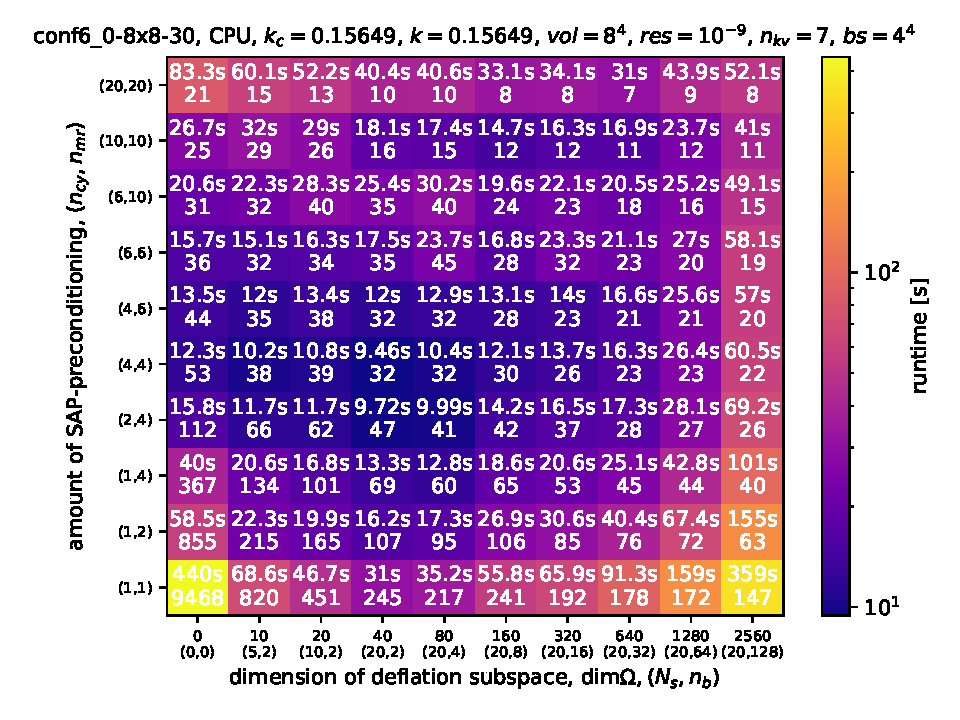
\includegraphics[width=1.0\textwidth]{plots/dfl_sap_gcr_conf6_0-8x8-30_8x8x8x8_k_0.15649}
    \caption{Time measurements for the \code{DFL\_SAP\_GCR} kernel on different matrices and configurations. The measurements where conducted on an Intel(R) 6130 @ 2.10GHz with 1.5 TB memory and an NVIDIA V100 (via PCIe) GPU with 16 GB memory.}
    \label{fig:dfl_sap_gcr0}
    \label{fig:dfl_sap_gcr_start}
    \label{fig:dfl_sap_gcr_conf6_0-8x8-30_8x8x8x8_k_0.15649}
\end{figure}

\begin{figure}[h]
    \centering
    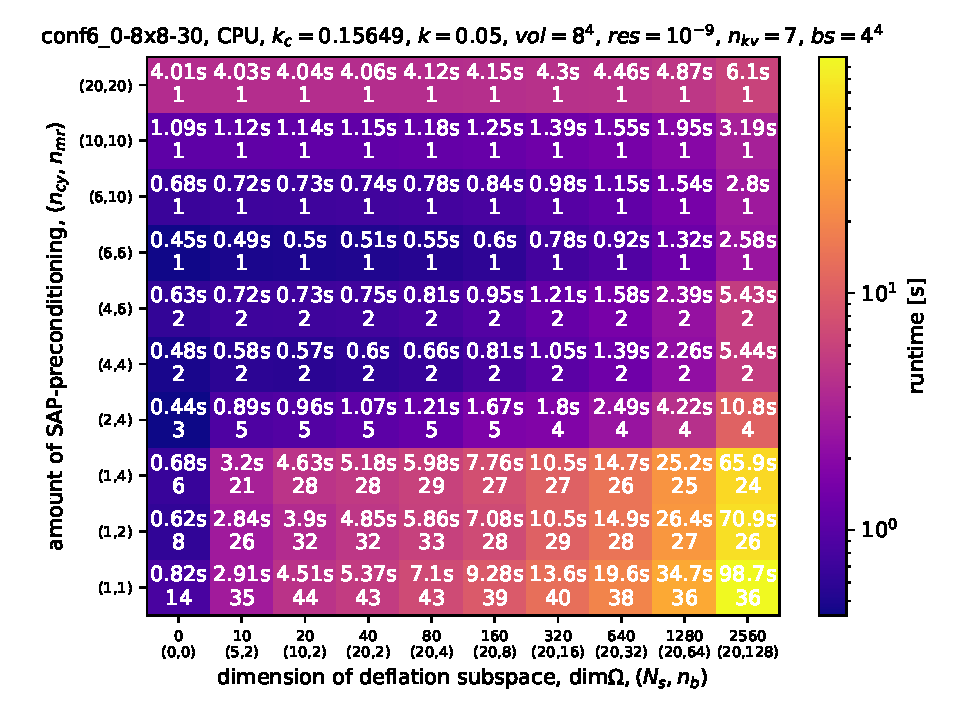
\includegraphics[width=1.0\textwidth]{plots/dfl_sap_gcr_conf6_0-8x8-30_8x8x8x8_k_0.05}
    \caption{Time measurements for the \code{DFL\_SAP\_GCR} kernel on different matrices and configurations. The measurements where conducted on an Intel(R) 6130 @ 2.10GHz with 1.5 TB memory and an NVIDIA V100 (via PCIe) GPU with 16 GB memory.}
    \label{fig:dfl_sap_gcr1}
    \label{fig:dfl_sap_gcr_conf6_0-8x8-30_8x8x8x8_k_0.05}
    \label{fig:dfl_sap_gcr_end}
\end{figure}

\subsubsection{Discussion of figures \ref{fig:dfl_sap_gcr_start} - \ref{fig:dfl_sap_gcr_end}}

The analysis was done on two Dirac-operators differing in their condition number. The operator in figure \ref{fig:dfl_sap_gcr_conf6_0-8x8-30_8x8x8x8_k_0.15649} is bad-conditioned, whereas in figure \ref{fig:dfl_sap_gcr_conf6_0-8x8-30_8x8x8x8_k_0.05} the operator is close to the identity. It is expected that both plots show some similarity. Namely the number of GCR-steps needed should decrease when going from the lower left point upward or to the right. There will be more precondtitioning and deflation in the mentioned directions, leading to fewer needed GCR-steps. The configuration at the top right should thus have the least GCR-steps out of all configurations. Although this does not imply that it is the fastest, because each GCR-step involves heavy amounts of Schwarz-preconditioning and the deflation subspace is the largest. Thus the top right configuration is the one most intense in computational effort per GCR-step.

Figure \ref{fig:dfl_sap_gcr_conf6_0-8x8-30_8x8x8x8_k_0.15649} is specially of interest, because the operator is in bad condition. The pattern we observe has a bowl-shape, where the minimum is at some certain configuration. Configurations in the neighborhood of the minimum perform similar. Starting from the minimum the runtime increases in every direction. The \num{100} configurations considered seem to sample the configuration space quite well. The plot shows that there is a non-trivial interplay between preconditioning and deflation. Clearly, solving the little equation reduces the components of the full residue associated to the low eigenmodes. On the other hand, preconditioning consolidates the spectrum around the value \num{1}. This compactification affects the high-modes more than the low-modes, leading to a reduction of the high-mode components of the full residue.

In contrast to the previous operator, the matrix in figure \ref{fig:dfl_sap_gcr_conf6_0-8x8-30_8x8x8x8_k_0.05} is well-conditioned. The plot tells us that in this case low-mode deflation is a waste of resources. Also repeating previous results from section \ref{sec:sap_gcr_results}, Schwarz-preconditioning should be kept within a tight limit for good conditioned systems. As stated previously, we expect the number of GCR-steps to decrease, when using larger deflation subspaces. On the contrary, when looking at the configuration $(n_{cy},n{mr}) = (1,1)$, we observe an \textit{increase} to the right instead. This suggests that too large deflation subspaces cause the solver to perform even worse, not only in runtime as it is with Schwarz-preconditioning, but also in the amount of GCR-steps, finally leading to a regression. This certain operator has a clustering of all its eigenvalues around $1$. The exact low-mode eigenspace is still of the same size as for the operator in figure \ref{fig:dfl_sap_gcr_conf6_0-8x8-30_8x8x8x8_k_0.15649}, but the low-eigenvalues are not clearly separated anymore from the bulk of eigenvalues\footnote{The operator does not satisfy equation \eqref{eq:separable} anymore.}. A separation is thus harder to achieve, making the deflation subspace arbitrary and the deflation of the full system unprogressive and expensive. In order for deflation to be effective in such a case, one needs to determine the $N_s$ bootstrap vectors more precisely by using more inverse iteration steps, making the generation of deflation subspace computationally more expensive. Obviously, the better alternative would be to drop deflation entirely and minimize Schwarz-preconditioning for such a system.

\subsubsection{Conclusion}

The runtime seems to be convex in the dimension of the deflation subspace. This suggests that the actual subspace of low eigenmodes lies approximately at the minimum of that convex curve. As a justification imagine that the actual subspace of low eigenmodes has dimension $d$, but the algorithm produced a subspace of dimension $d_1 \gg d$. This implies that the generated deflation subspace must contain high eigenmodes as well, making the little system more and more ill-conditioned. This results in longer runtimes, because the little equation has to be solved in every (outer) GCR-step. On the other hand, let's assume the algorithm generated a deflation subspace of dimension $d_2 \ll d$. Since only a few low eigenmodes could be split off, the deflated equation is still in bad condition. Also, although the little equation seems to be in good condition and very small in its dimension, thus solved fast, it contributes nearly nothing to the full solution. Again, this results in a longer runtime. Certainly, the perfect size for the deflation subspace is the size of the subspace of the (exact) low eigenmodes or a bit larger. Of importance is that the bulk of the low eigenmodes is contained in it.

Expectingly, the plots exhibit a bowl-shape, where the minimum gives the perfect balance between Schwarz-preconditioning and inexact low-mode deflation. The position of this minimum is certainly a property of the operator considered and depends on its condition number. If the number of low-modes can be upper bounded as tight as possible with little computational effort, then together with the adaptive variant of the \acrshort*{sapgcr} algorithm one obtains a powerful and versatile solver.

TODO

\section{Multi-shift Conjugate Gradient algorithm}

TODO

\begin{proposal}{MSCG in mixed precision}{mscg_mp}

TODO: \acrlong{mscg} in mixed precision. Currently only in binary64.

\end{proposal}

\section{Dirac operator}

\begin{comment}

The number of cycles in cg (or other solvers) do not scale with the lattice volume (times 12 which is the dimension of the matrix to solve), therefore the matrix becomes more sparse, the larger the lattice becomes. For very large lattice sizes D_dagger D starts to become proportional to the identity more and more, because the diagonal elements stay non-zero.

By ”Inversion” we mean inverting partially this matrix id est solving a set of equations of the type
Dψ=η (2.8)
where D and η are given and ψ is unknown. D is a 12N×12N complex matrix and η and ψ are 12N complex vectors. The solution is often called ”quark-propagator”. 

The gauge fields are SU(3) matrices. Inspecting their representations, they can be represented using 18, 12, 10 or 8 real numbers. The 8-representation involves 6 number between [-1,1] and 2 between [-pi,pi]. This is in all number ranges of all floating point types! In QUDA, they use 16-bit (or 8-bit) signed integers and cudaReadModeNormalizedFloat to convert to a binary32 in the range [-1,1].

\end{comment}

The Dirac-operator \eqref{eq:dwop} in openQxD is implmented in terms of the various gauge-fields $U_{\mu}(n)$, only these are stored in memory. In every HMC-trajectory the fields are updated, and the operator changes.

\subsection{Threaded Dirac-operator}

\label{sec:threads}

Modern processors today tend to have multiple cores. In order to benefit from that, two major programming models programmers are faced with are \acrshort{openmp} \cite{openmp45} and \acrshort{MPI} \cite{mpi}. Where MPI favors the scalability of large clusters with distributed memory, OpenMP favors speed of shared memory systems. Comparing the two solutions gives motivation to look at OpenMP more closely and consider using OpenMP for intra-node traffic. The goal is certainly a hybrid solution that keeps the scalbility of MPI, but exploits the speedup in shared memory systems using OpenMP, since on a single node, OpenMP seems to outperform MPI in most cases \cite{chan2011}.

\subsubsection{Setup}

The Dirac operator in single-precision was implemented as a variant utilizing threads according to the standard OpenMP in openQCD version 1.6 \cite{openqcd}. The performance of the operator was compared to the native implementation without threads. The runs were conducted on two different nodes having two vastly different processors, see tables \ref{tab:dop_omp_amd} and \ref{tab:dop_omp_intel}. On each node, \num{3} different lattice sizes were considered; $64^4$, $32^4$ and $16^4$. For each lattice size, there were many configurations $(n_r,n_{th})$ that were analyzed, $n_r$ being the number of ranks and $n_{th}$ the number of threads. Every configuration was executed \num{10} times, the average is printed in the table.

\subsubsection{Discussion}

\begin{table}
    \centering
    \begin{tabular}{ |p{1.5cm}||p{1cm}|p{1cm}|p{2cm}|p{2cm}|p{2cm}| }
        \hline
        & & & $64^4$ & $32^4$ & $16^4$ \\
        operator & $n_r$ & $n_{th}$ & time [s] & time [ms] & time [ms] \\
        \hline
        native & 256 & N/A & $1.06 \pm 0.02$ & $80.0 \pm 2.0$ & $9.53 \pm 0.33$ \\
        native & 128 & N/A & $1.06 \pm 0.01$ & $65.5 \pm 1.3$ & $6.63 \pm 0.73$ \\
        \hline
        omp & 128 & 1 & $1.12 \pm 0.06$ & $69.2 \pm 4.3$ & $6.32 \pm 0.13$ \\
        omp & 128 & 2 & $1.08 \pm 0.01$ & $71.8 \pm 6.0$ & $7.78 \pm 0.37$ \\
        omp & 128 & 4 & $1.09 \pm 0.01$ & $70.6 \pm 1.5$ & $9.90 \pm 2.68$ \\
        \hline
        omp & 64 & 1 & $1.54 \pm 0.08$ & $93.0 \pm 1.2$ & $7.14 \pm 0.17$ \\
        omp & 64 & 2 & $1.09 \pm 0.00$ & $66.6 \pm 3.9$ & $5.99 \pm 0.34$ \\
        omp & 64 & 4 & $1.07 \pm 0.01$ & $67.9 \pm 1.3$ & $8.39 \pm 0.40$ \\
        omp & 64 & 8 & $1.08 \pm 0.00$ & $70.7 \pm 1.7$ & $10.9 \pm 1.5$ \\
        \hline
        omp & 32 & 2 & $1.51 \pm 0.00$ & $94.1 \pm 0.3$ & $7.97 \pm 0.13$ \\
        omp & 32 & 4 & $1.09 \pm 0.00$ & $68.3 \pm 0.1$ & $6.87 \pm 0.24$ \\
        omp & 32 & 8 & $1.06 \pm 0.01$ & $72.6 \pm 0.8$ & $9.12 \pm 1.94$ \\
        omp & 32 & 16 & $1.09 \pm 0.00$ & $80.2 \pm 6.3$ & $11.7 \pm 0.7$ \\
        \hline
        omp & 16 & 4 & $1.60 \pm 0.01$ & $101 \pm 6$ & $8.83 \pm 0.10$ \\
        omp & 16 & 8 & $1.15 \pm 0.00$ & $79.9 \pm 0.8$ & $8.39 \pm 0.13$ \\
        omp & 16 & 16 & $1.13 \pm 0.01$ & $88.8 \pm 1.7$ & $10.9 \pm 1.0$ \\
        omp & 16 & 32 & $1.14 \pm 0.01$ & $92.7 \pm 1.8$ & $14.3 \pm 0.5$ \\
        \hline
        omp & 8 & 8 & $1.88 \pm 0.00$ & $131 \pm 7$ & $11.6 \pm 0.4$ \\
        omp & 8 & 16 & $1.26 \pm 0.01$ & $102 \pm 3$ & $10.7 \pm 0.1$ \\
        omp & 8 & 32 & $1.23 \pm 0.01$ & $110 \pm 7$ & $13.5 \pm 0.8$ \\
        omp & 8 & 64 & $1.30 \pm 0.03$ & $111 \pm 1$ & $19.7 \pm 0.6$ \\
        \hline
        omp & 4 & 16 & $2.01 \pm 0.01$ & $150 \pm 0$ & $14.3 \pm 0.1$ \\
        omp & 4 & 32 & $1.38 \pm 0.00$ & $124 \pm 1$ & $14.8 \pm 0.4$ \\
        omp & 4 & 64 & $1.36 \pm 0.02$ & $133 \pm 2$ & $19.4 \pm 0.4$ \\
        omp & 4 & 128 & $1.44 \pm 0.01$ & $134 \pm 4$ & $25.8 \pm 0.7$ \\
        \hline
        omp & 2 & 32 & $2.05 \pm 0.03$ & $169 \pm 6$ & $19.5 \pm 0.4$ \\
        omp & 2 & 64 & $1.50 \pm 0.05$ & $147 \pm 1$ & $19.6 \pm 0.6$ \\
        omp & 2 & 128 & $1.43 \pm 0.01$ & $167 \pm 3$ & $25.3 \pm 1.4$ \\
        omp & 2 & 256 & $1.49 \pm 0.03$ & $165 \pm 7$ & $34.0 \pm 1.3$ \\
        \hline
        omp & 1 & 64 & $2.17 \pm 0.00$ & $142 \pm 0$ & $12.5 \pm 0.2$ \\
        omp & 1 & 128 & $2.18 \pm 0.01$ & $144 \pm 3$ & $15.2 \pm 0.5$ \\
        omp & 1 & 256 & $2.19 \pm 0.01$ & $157 \pm 6$ & $17.4 \pm 0.8$ \\
        omp & 1 & 512 & $2.35 \pm 0.01$ & $171 \pm 3$ & $53.4 \pm 5.3$ \\
        \hline
    \end{tabular}
    \caption{\num{10} consecutive invocations of the single precision Dirac-operator \code{Dw()} on random fields in openQCD version 1.6. The table shows runs with different rank/thread configurations $(n_r, n_{th})$ on differnt lattice sizes. The lattice size refers to the total lattice size on the node. The node consisted of \num{2} NUMA nodes, \num{2} sockets with each an AMD EPYC 7742 processor @ 2.25GHz with \num{64} physical cores per socket and \num{2} threads per core; in total \num{256} logical CPUs, with 512GB of memory. The cache sizes of one processor are L1 data: 2MB, L1 instruction: 2MB, L2: 32MB, L3: 256MB. L1 data: 2MB ($64 \times 32$KB), L1 instruction: 2MB ($64 \times 32$KB), L2: 32MB ($64 \times 512$KB), L3: 256MB ($16 \times 16$MB).}
    \label{tab:dop_omp_amd}
\end{table}

In table \ref{tab:dop_omp_amd} the number of physical and logical CPUs was a power of two, therefore in both cases - native and with threads - all logical CPUs in the node could be utilized. In general, the best runtimes were achieved with the native operator. The only exception for the $16^4$ lattice was the run with \num{64} ranks and \num{2} threads per rank. With that lattice size the whole gauge-field configuration fits into L2 cache of one processor (see table \ref{tab:lattice_sizes}), making consecutive runs very fast. Specially for the threaded variant, it can be seen that with double the amounts of threads the problem is not solved in half the time. This suggests that the overhead for dealing with threads is not negligible, and the threaded variant is in need of improvement. It should be seen as a first working step towards hyper-threading. On the other hand, also the native implementation lacks an ideal strong scaling by looking that the first two rows. Generally the runs with only \num{128} ranks are faster than the runs utilizing every of the \num{256} logical cores. This holds for all considered lattice sizes. Let's concentrate on the most interesting lattice size $64^4$. The threaded variant brings no benefit compared to the native one, but there are configurations that are comparable in runtime, namely the ones with $(n_r, n_{th})=(64,4)$ as well as $(32,8)$. Both utilize all logical cores of the node. Improving the threaded implementation can therefore lead to a speedup increase (see conclusion). Generally the less ranks, the worse the performance becomes. This can be explained by false sharing among the threads and ignorance concerning NUMA-effects when omplementing the the threaded variant.

Table \ref{tab:dop_omp_intel} shows a differnt picture. Most notable in the analysis is the fact that the total number of physical and logical cores was \textit{not} a power of two on this node. This makes it difficult to utilize all resources of the node using the native implementation. This fact is reflected by the results. The threaded variant has substantial performance increases compared to the best native pure-MPI implementation. Specially the configurations with ranks and threads being $(n_r, n_{th})=(16,7)$, $(8,14)$ and $(4,14)$ perform best. The reason for this lies in the complicated association of cores to NUMA-domains. The node uses \num{4} NUMA-domains, where the logical cores are associated to NUMA-domains in a non-trival manner (see listings \ref{lst:lscpu}). \num{14} logical cores share an L3 cache. This explains why the mentioned configurations with \num{14} threads perform well. The jobs were disposed in a way that the \num{14} threads are bound to physical cores\footnote{With the OpenMP environment variable \code{OMP\_PLACES=cores}.} with the same L3 cache.

\begin{figure} % wrap into a figure such that the whole snippet is on the same page
\begin{lstlisting}[
    language=C,
    numbers=none,
    label=lst:lscpu,
    caption={Output of \code{lscpu -e}. Notice the association of logical cores (first column) to NUMA-domains (second column). The fourth column denotes the physical core. Each NUMA-domain has \num{14} logical cores, where core \num{0} and \num{56} belong to physical core \num{0} sharing their L1 and L2 cache on NUMA node \num{0}, logical cores \num{1} and \num{57} belong to physical core \num{1} on NUMA node \num{0} sharing L1 and L2 cache and so on. The L3 cache is shared on nodes \num{0}-\num{13}, \num{14}-\num{27}, and so on.}
]
$ lscpu -e
CPU NODE SOCKET CORE L1d:L1i:L2:L3 ONLINE
0   0    0      0    0:0:0:0       yes
1   0    0      1    1:1:1:0       yes
2   0    0      2    2:2:2:0       yes
3   0    0      3    3:3:3:0       yes
4   0    0      4    4:4:4:0       yes
[...]
13  0    0      13   13:13:13:0    yes
14  1    1      14   14:14:14:1    yes
[...]
27  1    1      27   27:27:27:1    yes
28  2    2      28   28:28:28:2    yes
[...]
41  2    2      41   41:41:41:2    yes
42  3    3      42   42:42:42:3    yes
[...]
51  3    3      51   51:51:51:3    yes
52  3    3      52   52:52:52:3    yes
53  3    3      53   53:53:53:3    yes
54  3    3      54   54:54:54:3    yes
55  3    3      55   55:55:55:3    yes
56  0    0      0    0:0:0:0       yes
57  0    0      1    1:1:1:0       yes
58  0    0      2    2:2:2:0       yes
59  0    0      3    3:3:3:0       yes
60  0    0      4    4:4:4:0       yes
[...]
69  0    0      13   13:13:13:0    yes
70  1    1      14   14:14:14:1    yes
[...]
83  1    1      27   27:27:27:1    yes
84  2    2      28   28:28:28:2    yes
[...]
97  2    2      41   41:41:41:2    yes
98  3    3      42   42:42:42:3    yes
[...]
107 3    3      51   51:51:51:3    yes
108 3    3      52   52:52:52:3    yes
109 3    3      53   53:53:53:3    yes
110 3    3      54   54:54:54:3    yes
111 3    3      55   55:55:55:3    yes
\end{lstlisting}
\end{figure}

\begin{table}
    \centering
\begin{tabular}{ |p{1.5cm}||p{1cm}|p{1cm}|p{2cm}|p{2cm}|p{2cm}| }
    \hline
    & & & $64^4$ & $32^4$ & $16^4$ \\
    operator & $n_r$ & $n_{th}$ & time [s] & time [ms] & time [ms] \\
    \hline
    native & 64 & N/A & $0.0 \pm 0$ & $280 \pm 0$ & $21.6 \pm 7.5$ \\
    native & 32 & N/A & $0.0 \pm 0$ & $538 \pm 2$ & $30.3 \pm 0.1$ \\
    native & 16 & N/A & $0.0 \pm 0$ & $450 \pm 3$ & $28.2 \pm 0.1$ \\
    omp & 64 & 1 & $0.0 \pm 0$ & $298 \pm 0$ & $25.1 \pm 14.3$ \\
    omp & 64 & 2 & $0.0 \pm 0$ & $304 \pm 14$ & $24.3 \pm 6.2$ \\
    omp & 64 & 4 & $0.0 \pm 0$ & $300 \pm 0$ & $22.0 \pm 5.0$ \\
    omp & 64 & 8 & $0.0 \pm 0$ & $303 \pm 0$ & $24.9 \pm 4.0$ \\
    omp & 32 & 1 & $0.0 \pm 0$ & $581 \pm 1$ & $33.7 \pm 0.1$ \\
    omp & 32 & 2 & $0.0 \pm 0$ & $583 \pm 1$ & $34.2 \pm 0.2$ \\
    omp & 32 & 4 & $0.0 \pm 0$ & $584 \pm 1$ & $35.4 \pm 0.1$ \\
    omp & 32 & 7 & $0.0 \pm 0$ & $590 \pm 0$ & $37.1 \pm 0.1$ \\
    omp & 16 & 2 & $0.0 \pm 0$ & $269 \pm 2$ & $18.8 \pm 0.1$ \\
    omp & 16 & 4 & $0.0 \pm 0$ & $290 \pm 0$ & $18.3 \pm 0.1$ \\
    omp & 16 & 7 & $0.0 \pm 0$ & $190 \pm 1$ & $14.1 \pm 0.1$ \\
    omp & 16 & 14 & $0.0 \pm 0$ & $259 \pm 1$ & $20.8 \pm 0.1$ \\
    omp & 8 & 4 & $0.0 \pm 0$ & $299 \pm 2$ & $21.9 \pm 0.0$ \\
    omp & 8 & 8 & $0.0 \pm 0$ & $318 \pm 0$ & $21.7 \pm 0.1$ \\
    omp & 8 & 14 & $0.0 \pm 0$ & $217 \pm 9$ & $17.7 \pm 0.5$ \\
    omp & 8 & 28 & $0.0 \pm 0$ & $217 \pm 0$ & $20.6 \pm 0.1$ \\
    omp & 4 & 7 & $0.0 \pm 0$ & $353 \pm 1$ & $25.2 \pm 0.1$ \\
    omp & 4 & 14 & $0.0 \pm 0$ & $225 \pm 8$ & $18.0 \pm 0.1$ \\
    omp & 4 & 28 & $0.0 \pm 0$ & $238 \pm 1$ & $20.0 \pm 0.2$ \\
    omp & 4 & 56 & $0.0 \pm 0$ & $244 \pm 1$ & $25.3 \pm 0.1$ \\
    omp & 2 & 28 & $0.0 \pm 0$ & $320 \pm 0$ & $21.8 \pm 0.1$ \\
    omp & 2 & 56 & $0.0 \pm 0$ & $326 \pm 1$ & $23.7 \pm 0.1$ \\
    omp & 2 & 112 & $0.0 \pm 0$ & $340 \pm 2$ & $33.7 \pm 1.2$ \\
    omp & 1 & 56 & $0.0 \pm 0$ & $301 \pm 1$ & $17.3 \pm 0.1$ \\
    omp & 1 & 112 & $0.0 \pm 0$ & $314 \pm 1$ & $18.6 \pm 0.2$ \\
    omp & 1 & 224 & $0.0 \pm 0$ & $338 \pm 2$ & $36.3 \pm 0.2$ \\
    \hline
\end{tabular}

    \caption{\num{10} consecutive invocations of the single precision Dirac-operator \code{Dw()} on random fields in openQCD version 1.6. The table shows runs with different rank/thread configurations $(n_r, n_{th})$ on differnt lattice sizes. The lattice size refers to the total lattice size on the node. The node consisted of \num{4} NUMA nodes, \num{4} sockets with each an Intel(R) E7-4830 v4 @ 2.00GHz with \num{14} physical cores per socket and \num{2} threads per core; in total \num{112} logical CPUs, with 2TB of memory. The cache sizes of one processor are L1 data: 448KB ($14 \times 32$KB), L1 instruction: 448KB ($14 \times 32$KB), L2: 3.5MB ($14 \times 256$KB), L3: 35MB ($1 \times 35$MB).}
    \label{tab:dop_omp_intel}
\end{table}

\begin{table}
\centering
    \begin{tabular}{ |p{1cm}|p{2cm}|p{2cm}| }
        \hline
        lattice & gauge-field & quark-field \\
        \hline
        $16^4$ & 18MB & 6MB \\
        $32^4$ & 288MB & 96MB \\
        $64^4$ & 4608MB & 1536MB \\
        \hline
    \end{tabular}
    \caption{Sizes in memory of the gauge- and quark-fields in terms of lattice sizes.}
    \label{tab:lattice_sizes}
\end{table}

\subsubsection{Conclusion}

The threaded variant is usefull on machines where the number of logical or physical cores is not a power of two, or can somehow not be fully utilized by the pure-MPI implementation. Since in openQCD (and openQxD) the number of ranks in one direction can only be $2,4,6,\dots$ and the lattice size in one direction can only be $4,6,8,\dots$, these numbers are pretty limited for a given lattice size and a processor where the number of CPUs is not a power of two. Utilizing the whole node is not always possible\footnote{For example the node in table \ref{tab:dop_omp_intel}, where only a maximum of \num{64} from a total of \num{112} logical cores could be utilized.}. In such a case, the threaded operator can utilize the whole node, because the number of threads per rank is arbitrary.

When implementing threads, it is important to write code aware of NUMA effects. In the above implementation there are certainly performance degradations due to NUMA effects and false sharing. It was tried to honour the first-touch policy as often as possible, by initializing the involved arrays with a parallel for loop, just as they are accessed later in the main loop\footnote{See line 1295ff in \code{modules/dirac/Dw.c} in \cite{openqcd_threads}} of the Dirac-operator. Although a certain amount of false sharing was not preventable without significantly changing the original main loop.

Another peculiarity of the above implementation was that in \code{deo()} the \num{8} directions of the gauge-fields had to be separately locked for every lattice point, because the output vector was written to in these code segments leading to race conditions without locking. The initialization and de-initialization of \code{VOLUME/2} locks involes a non-negligible overhead in every invocation of the Dirac-operator.

\begin{proposal}{The Dirac-operator with threads}{dop_threads}

The analysis in section \ref{sec:threads} shows that a version of the Dirac-operator employing threads can improve performance as well.

For future refinements of the threaded implementation one can concentrate on false sharing of the current implementation. For example in the main loop, instead of consecutively looping over the elements that are being read, loop over the elements that are being written (the output spinor) in a way that only a (consecutive) slice of the output spinor is written in each iteration. Each thread then has its own constant equally-sized slice to write to, without having race conditions with other threads. This would not need any expensive locking anymore. Also, this implies to use \code{schedule(static)} and the same boundaries in all parallel for loops, such that a thread always gets the same loop slice within different for loops. The current test-implementation obeys that. A certain amount of false sharing is not preventable without changing the loop as described above. In the parts of the code where the output spinor \code{r} is written consecutively (\code{r+i} or \code{r+VOLUME/2+i}) only true sharing appears, because \code{r} was initialized in the exact same way (first touch policy). But within \code{deo()}, \code{r} is written on arbitrary offsets, leading to false sharing.

\end{proposal}

\begin{comment}

threads:

* machines with no power of 2 as number of logical or physical cores
* NUMA-aware coding -> initialize the arrays in the same way as accessing them -> first touch policy
* false sharing among threads -> when possible access only elements that are "near" (in the numa domain)
* locking of the 8 directions from each lattice point -> race condition. Total of 2*VOLUME locks, mostly neglectible

future:
1) instead of looping over the elements that are being read, loop over the elements that are being written (the output spinor) in a way that only a (consecutive) slice of the output spinor is written in each iteration. Each thread then has its own constant equal-sized slice. This would imply to use schedule(static) and the same boundaries in all parallel loops, such that a threads always gets the same loop slice. The current test-implementation obeys that.
2) a certain amount of false sharing was not preventable without changing the loop as described in point 1). In the parts of the code where the output spinor r is written consecutively (r+i or r+VOLUME/2+i) only true sharing appears, because r was initialized in the exact same way (first touch policy).

\end{comment}

\subsection{Dirac-operator representations}

\begin{proposal}{Representation of the Dirac-operator}{dop_reps}
For the implementation of the Dirac-operator on the GPU, the software library QUDA \cite{clark2010} is a good sample. To improve the performance of their Dirac-operator, the authors of QUDA used a representation of the SU(3)-fields with \num{8} real numbers, a gauge transformation to make almost all of the gauge fields in temporal direction to the identity-matrix and a change of basis in the $\gamma$-matrices, such that one of the four matrices has a very simple form. The most interesting one is probably the SU(3)-representation with only \num{8} real numbers. In openQxD \footnote{See line 43 in \code{include/su3.h} in \cite{openqxd}.} the struct \code{su3\_dble} representing a SU(3)-gauge-field consists of \num{18} double precision numbers. The C-macro for a matrix-matrix multiplication of 2 such \code{su3\_dble} \footnote{See line 490ff in \code{include/su3.h} in \cite{openqxd}.} consists of $18 \cdot 12$ FLOPs, $2 \cdot 18$ loads and $18$ stores. Using \gls{binary64}, the arithmetic intensity is $I = 0.5$ FLOPs per byte, making the problem memory-bound.

Since the rows and columns of SU(3)-matrices form a orthonormal basis of $\mathbb{C}^3$, one representation of such matrices can hold only the first two rows or columns and the third row or column is calculated as the vector product of the former two \cite{deforcrand1985}. This is a representation with \num{12} real numbers. A matrix-matrix multiplication of 2 such matrices ends up in $270$ FLOPs, $2 \cdot 12$ loads and $12$ stores. This results in an arithmetic intensity of $I = 0.9375$ FLOPs per byte using \gls{binary64} - sill memory bound.

If the representation of a SU(3)-gauge-field would be chosen such that the struct contains only \num{10} numbers \cite{bunk1986}, then a matrix $A \in SU(3)$ would be represented as ($a_{ij} \in \mathbb{C}$)

\begin{align*}
    A =
    \begin{pmatrix}
    a_{11} & a_{12} & a_{13} \\
    a_{21} & a_{22} & a_{23} \\
    a_{31} & a_{32} & a_{33} 
    \end{pmatrix}
    &= 
    \begin{pmatrix}
    1 & 0 & 0 \\
    0 &   N a_{31}^{*} & N a_{21} \\
    0 & - N a_{21}^{*} & N a_{31}
    \end{pmatrix}
    \begin{pmatrix}
    a_{11} & a_{12} & a_{13} \\
    0 & - N a_{13}^{*} & - N a_{12}^{*} \\
    \frac{1}{N} & - N a_{11}^{*} a_{12} & - N a_{11}^{*} a_{13}
    \end{pmatrix} \\
    &= 
    \begin{pmatrix}
    a_{11} & a_{12} & a_{13} \\
    a_{21} & -N^2 \left( a_{13} a_{31}^{*} + a_{11}^{*} a_{12} a_{21} \right) & -N^2 \left( a_{12}^{*} a_{31}^{*} + a_{11}^{*} a_{13} a_{21} \right) \\
    a_{31} & -N^2 \left( a_{13}^{*} a_{21}^{*} + a_{11}^{*} a_{12} a_{31} \right) & -N^2 \left( a_{12}^{*} a_{21}^{*} + a_{11}^{*} a_{13} a_{31} \right) 
    \end{pmatrix}
\end{align*}

where $N \coloneqq \left(1 - \abs{a_{11}}^2 \right)^{-\frac{1}{2}}$. Notice that this representation has a singularity at $\abs{a_{11}}=1$. The \num{5} complex numbers $a_{11}, a_{12}, a_{13}, a_{21}, a_{31}$ are subject of the orthonormality constraints

\begin{align}
  \abs{a_{11}}^2 + \abs{a_{12}}^2 + \abs{a_{13}}^2 = \abs{a_{11}}^2 + \abs{a_{21}}^2 + \abs{a_{31}}^2 = 1, \label{eq:su3_orth_constr}
\end{align}

leading to the observation that all \num{12} real numbers are in the set $[-1, 1].$

Finally, in a minimal representation of $8$ real numbers \cite{bunk1986}, can be obtained using the constraint above \eqref{eq:su3_orth_constr}. If we write $a_{ij} = x_{ij} + i y_{ij}$ with $x_{ij}, y_{ij} \in \mathbb{R}$ we can eliminate \num{2} further numbers. One (of many) choices could be

\begin{align}
  y_{31} &= \sqrt{1 - \abs{a_{11}}^2 - \abs{a_{21}}^2 - \abs{x_{31}}^2} \\
  y_{13} &= \sqrt{1 - \abs{a_{11}}^2 - \abs{a_{13}}^2 - \abs{x_{13}}^2}.
\end{align}

Using this, only $a_{11}, a_{12}, a_{21}$ and the real parts of $a_{13}$ and $a_{31}$ need to be stored in memory. For a breakdown of the different arithmetic intensities of the representations, see table \ref{tab:ai_su3}.

\begin{table}[H]
\centering
    \begin{tabular}{ |p{1.2cm}|p{2cm}|p{2cm}|p{2cm}|  }
        \hline
        \multicolumn{4}{|c|}{Arithmetic intensities in FLOPs per byte} \\
        \hline
        Reals & I(binary64) & I(binary32) & I(binary16) \\
        \hline
        18  & 0.5    & 1       & 2      \\
        12  & 0.9375 & 1.875   & 3.75   \\
        10  & 1.3667 & 2.7333  & 5.4667 \\
        8   & 1.9115 & 3.8229  & 7.6458 \\
        \hline
    \end{tabular}
    \caption{Arithmetic intensities of SU(3) representations with different requirement for real numbers for a matrix-matrix multiplication. In the calculation of the intensities a FLOP-count of \num{6} was used for the square root of a floating point number and previous results were reused instead of recalculating.}
    \label{tab:ai_su3}
\end{table}
    
In table \ref{tab:dw_dble} one invocation of \code{Dw\_dble()} was called and the macros from \code{su3.h} where counted.

\begin{table}[H]
\centering
    \begin{tabular}{ |p{1.2cm}|p{4cm}|p{1.2cm}|p{1.2cm}|p{1.2cm}|p{1.2cm}|  }
        \hline
        \multicolumn{6}{|c|}{One invocation of \code{Dw\_dble()}} \\
        \hline
        \# calls & macro name & I(18) & I(12) & I(10) & I(8) \\
        \hline
        61440 & \code{\_vector\_add\_assign()}    & 0.0416 & 0.0416 & 0.0416 & 0.0416 \\
        24576 & \code{\_su3\_multiply()}          & 0.3    & 0.625 & 0.9323 & 1.0989 \\
        24576 & \code{\_su3\_inverse\_multiply()} & 0.3    & 0.625 & 0.9323 & 1.0989 \\
        12288 & \code{\_vector\_add()}            & 0.0416 & 0.0416 & 0.0416 & 0.0416 \\
        12288 & \code{\_vector\_i\_add()}         & 0.0416 & 0.0416 & 0.0416 & 0.0416 \\
        12288 & \code{\_vector\_i\_add\_assign()} & 0.0416 & 0.0416 & 0.0416 & 0.0416 \\
        12288 & \code{\_vector\_sub()}            & 0.0416 & 0.0416 & 0.0416 & 0.0416 \\
        12288 & \code{\_vector\_i\_sub()}         & 0.0416 & 0.0416 & 0.0416 & 0.0416 \\
        12288 & \code{\_vector\_sub\_assign()}    & 0.0416 & 0.0416 & 0.0416 & 0.0416 \\
        12288 & \code{\_vector\_i\_sub\_assign()} & 0.0416 & 0.0416 & 0.0416 & 0.0416 \\
        \hline
    \end{tabular}
    \caption{Number of C macro calls for one call of \code{Dw\_dble()} on a $8^4$ local lattice with $4$ ranks.}
    \label{tab:dw_dble}
\end{table}

When modifying the C structs \code{su3} or \code{su3\_dble}, one has to search the whole codebase for typecasts of these structs to other types, because such casts rely on guarantees of the ANSI C standard about memory layouts of fields within the struct. When changing the struct, the layout in memory is altered as well, making the typecast to another (unchanged) struct faulty \cite{siff1999}.

\begin{comment}
A necessary condition for GPU acceleration to be advantageous is that the benefit of doing work on the GPU exceeds the cost of getting the data there.
\end{comment}

\end{proposal}


\section{GPU Implementation}

There are multiple possibilities how to implement GPU-utilisation into the current state of the code. The proposals be divided roughly into 2 categories.

\begin{itemize}
    \item Use the resources of the GPU to process a larger lattice in the same time as before.
    \item Use the resources of the GPU to process the same lattice, but faster than before.
\end{itemize}

\begin{proposal}{GPU Implementation Variant 1}{gpu_implementation1} % ref with pp:gpu_implementation1

Keeping the results in mind (figures \ref{fig:sap_gcr_start} - \ref{fig:sap_gcr_end}) that the pure GPU implementation of the \code{SAP\_GCR} was by far the fastest, it makes sense to associate a local lattice to each GPU - so to treat a GPU as an additional rank with its own local lattice. Each GPU would then act as another rank and the full lattice can be extended by as many local lattices as there are available GPUs. Some nodes might have GPUs, some not. Each GPU has a \df{bystander process} running on the CPU. Process contexts associated to a GPU (CPU) are from now on called \df{GPU ranks} (\df{CPU ranks}). The bystander process will not need a lot of CPU load, since it only hosts control and informational variables and is not involved in any calculations. The communication from a GPU rank to another rank (CPU or GPU) in the system can be done either via the bystander process or via direct injection into the network bypassing the CPU and the bystander process. The former case will not need a change of the MPI communication code among ranks. Since the communication will only take negligible computational effort on the bystander process, it will not \textit{steal} much from the CPU ranks running on the same node. Let me give an example: Let' s assume the application runs on one single node with \num{8} cores and \num{4} GPUs attached to it. This would involve \num{8} CPU ranks (separate processes) and \num{4} GPU ranks with in total \num{4} (separate) bystander processes. Technically the machine is over-subscripted and the operating system needs to schedule the processes. But since the bystander processes will be in sleeping state most of the time, this will not (or only negligibly) degrade the performance of the \num{8} CPU ranks.

\begin{itemize}
    \item Advantage: The application can run on hybrid machines in the sense that some nodes can have GPUs attached to them and others don't.
    \item Disadvantage: The full system consists of two types of ranks - GPU ranks and CPU ranks. Inevitably, either the GPU or the CPU ranks will be faster on the same local lattice size. This means that either the GPUs or the CPUs will have to wait for the others to finish. Utilisation of resources is not perfect.
\end{itemize}

\end{proposal}

\begin{proposal}{GPU Implementation Variant 2}{gpu_implementation2} % ref with pp:gpu_implementation2

Since the GPUs are fast on the solver algorithms, a pure GPU implementation of all currently implemented solvers \footnote{\acrshort{cgne}, \acrshort{mscg}, \acrshort{sapgcr} and \acrshort{dflsapgcr}} can lead to a significant speed up of the program.

\begin{itemize}
    \item Advantage: Only the small subset of solver algorithm code has to be changed.
    \item Disadvantage: The Dirac-operator has to be held in the main memory as well as in the GPU memory. Both need to be in sync. This will lead to a lot of intra-node traffic, which itself should not be a problem. The Dirac-operator is stored in terms of its gauge-fields. They will be redundant and thus the full amount of GPU and CPU memory us not optimally utilised.
    \item Disadvantage: Since the solvers run on the GPUs, the CPUs will be stale during that time (although the waiting time will be smaller than the time they would need to run the solvers themselves). In the HMC-calculations done on the CPUs, the GPUs will be stale. Again the full potential of performance is not utilised.
\end{itemize}

\end{proposal}

\begin{proposal}{GPU Implementation Variant 3}{gpu_implementation3} % ref with pp:gpu_implementation3

If the problem is split among CPU ranks and GPU ranks, one will always have the waiting problem in the sense that either the CPU or the GPU ranks will have to wait for the others to complete (see proposal \ref{pp:gpu_implementation1}). In order for the GPU to speed up the process, every rank should receive the same amount of help from the GPUs. Then every rank solves the same problem faster. This is possible if all nodes participating in the calculation share the same specifications, the same number GPUs (not zero) and the same amount of memory. Let's assume this is given. Starting with a hybrid implementation as in proposal \ref{pp:sap_mr_gpu}, only the blocked problems are solved on the GPU and the internal color boundary operator as well as the full Dirac-operator are performed on the CPU as usual (see figures \ref{fig:sap_gcr_start} - \ref{fig:sap_gcr_end}, diamonds; \textcolor{cbrown}{$\diamond$}, \textcolor{cred}{$\diamond$}, \textcolor{cblue}{$\diamond$}). This means that \textit{all} blocked problems of all ranks on a single node are solved (or rather \code{nmr} MR-steps are performed) on the GPUs of that node. During that time the CPUs are stale. To solve this problem, we can use the fact that all blocks of the same color are independent of each other. So, not all blocks need to be transferred to the GPU - some of them can still reside and be processed in the current rank on the CPU. The work here should be divided such that both - CPU and GPU - need approximately the same amount of time for the processing of their blocks. The question on \textit{how} to divide the blocks still remains. It is evident that the GPU might be able to process more blocks than the CPU rank in the same time, but this highly depends on its occupation. A robust solution might implement the division of blocks in an adaptive manner.

\begin{itemize}
    \item Advantage: This proposal can be a good starting point from where to go further.
    \item Disadvantage: The GPU is only utilised in one part of one solver algorithm, else the GPU is stale.
\end{itemize}


\end{proposal}

\section{Algorithm-independent considerations}

\begin{proposal}{Choice of starting vectors}{starting_vector} % ref with pp:starting_vector

\begin{comment}
label:sick_proposal

Sick proposal: For every calculation of A^-1 x for a given x, we need to solve Ay=x iteratively. This is done in every trajectory step in HMC. Throughout the whole process this is done 1000s of times, always for a different x. Let x_1, ..., x_n be such x's. if for two such x's |x_i - x_j| = small, then

A yi = xi ~ xj = A yj

and therefore 

xi ~ xj => A^-1 xi ~ A^-1 xj => yi ~ yj

The solution can be recycled. Also if |x_i - x_j| = small, but not small enough for the above, ans assuming that the solution to Ayi=xi is present to a certain precision, then one could solve for 

Ayj=xj, with starting vector yi, and after few iterations obtain yj to certain precision.


\end{comment}

During a simulation, a lot of linear systems of equation of the type $A \vec{x} = \vec{b}$ have to be solved. Most solving algorithms have the possibility to choose a initial starting vector $\vec{x}_0$ from where to start the iterative process (see definition \ref{eq:cg:start} for example). Consider the sequence of matrices and source vectors for which the linear system of equations should be solved $\{A_1, \vec{b}_1\}, \{A_2, \vec{b}_2\}, \dots, \{A_n, \vec{b}_n\}$ and the matrix $A$ not changing very much among steps ($A_i \approx A_j$). If the difference $\norm{\vec{b}_i - \vec{b}_j}$ is small, then the difference of the solution vectors $\norm{\vec{x}_i - \vec{x}_j}$ can be expected to be small too. Assuming that the system $A_i \vec{x}_i = \vec{b}_i$ is already solved, the iterative solver for $A_j \vec{x}_j = \vec{b}_j$ can use $\vec{x}_i$ as its initial starting vector and reduce the amount of steps needed to solve the latter system.

\end{proposal}

\section{Summary}

TODO

\section{Future}

\begin{comment}

* MSCG in mixed precision (currently it's only in double)

\end{comment}

\newpage

\bibliography{include/references}

\bibliographystyle{abbrv}

\newpage

%\appendix
\begin{appendix}

\section*{Appendices} % new subsection without number
\addcontentsline{toc}{section}{Appendices} % Add "Appendices" to toc
\renewcommand{\thesubsection}{\Alph{subsection}} % change number of subsections to alphanumeric (A, B, C, ..)

% Change numberig of theorems according to subsection (not section): A.1, B.2, C.4, etc...
\renewcommand{\thetheorem}{\Alph{subsection}.\arabic{theorem}}
\renewcommand{\thedefinition}{\Alph{subsection}.\arabic{definition}}
\renewcommand{\thecorollary}{\Alph{subsection}.\arabic{corollary}}
\renewcommand{\theexample}{\Alph{subsection}.\arabic{example}}
\renewcommand{\theprop}{\Alph{subsection}.\arabic{prop}}
\renewcommand{\thelemma}{\Alph{subsection}.\arabic{lemma}}

\subsection{Proofs}
\label{sec:proofs}

\begin{prop}[Gaussian integral formula]

\label{prop:gauss_integral}

Let $B$ be a hermitian, invertible $n \times n$-matrix and $z_i \in \mathbb{C}$, for $i = 1, \dots, n$, then

\begin{align*}
  \prod_{k=1}^n \int d z_k^{\star} d z_k \exp( - \sum_{i,j=0}^n z_i^{*} B_{ij} z_j ) = \pi^n (\det B)^{-1}.
\end{align*}

\end{prop}

\begin{proof}

TODO

\end{proof}

\begin{theorem}[Inverse Power Method]

\label{thm:inverse_power_method}

Let $n \in \mathbb{N}$, $A$ be a invertible $n \times n$-matrix with a smallest eigenvalue $\abs{\lambda_1} < \abs{\lambda_2} \leq \dots \leq \abs{\lambda_n}$ and eigenvectors $\vec{v}_i$. Let $\vec{b}_0 = \sum_{i=1}^n c_i \vec{v}_i$ be an arbitrary (random) vector with support in the smallest eigenspace, ie. $c_1 \neq 0$. Then

\begin{align*}
  (A^{-1})^k \vec{b}_0 \xrightarrow{k\rightarrow\infty} \frac{c_1}{\lambda_1^k} \vec{v}_1
\end{align*}

is proportional to the eigenvector cooresponding to the smallest eigenvalue.

\end{theorem}

\begin{proof}

\begin{align*}
  (A^{-1})^k \vec{b}_0 &= \sum_{i=1}^n c_i (A^{-1})^k \vec{v}_i\\
  &= \sum_{i=1}^n \frac{c_i}{\lambda_i^{k}} \vec{v}_i\\
  &= \frac{c_1}{\lambda_1^k} \left( \vec{v}_1 + \sum_{j=2}^n \left(\frac{\lambda_1}{\lambda_j}\right)^k \frac{c_j}{c_1} \vec{v}_j \right).
\end{align*}

Since $\abs{\lambda_1} < \abs{\lambda_j}$, for $j \ge 1$, $\left(\frac{\lambda_1}{\lambda_j}\right)^k \to 0$ for $k \to \infty$.

\end{proof}

\begin{corollary}[]

\label{cor:inverse_power_method}

Let $A$ be as in theorem \ref{thm:inverse_power_method}, but with $n > m$ smallest eigenvalues of approximately the same magnitude $\abs{\lambda_1} \approx \abs{\lambda_2} \approx \dots \approx \abs{\lambda_{m}} \le \abs{\lambda_{m+1}} \leq \dots \leq \abs{\lambda_n}$. Then

\begin{align*}
  (A^{-1})^k \vec{b}_0 \xrightarrow{k\rightarrow\infty} \sum_{i=1}^m d_i \vec{v}_i
\end{align*}

is a linear combination of eigenvectors cooresponding to the $m$ smallest eigenvalues.

\end{corollary}

\begin{proof}

By the same analysis as in the proof of theorem \ref{thm:inverse_power_method},

\begin{align*}
  (A^{-1})^k \vec{b}_0 &= \frac{c_1}{\lambda_1^k} \left( \vec{v}_1 + \sum_{j=2}^m \underbrace{\left(\frac{\lambda_1}{\lambda_j}\right)^k}_{\approx 1} \frac{c_j}{c_1} \vec{v}_j + \sum_{l=m+1}^n \left(\frac{\lambda_1}{\lambda_l}\right)^k \frac{c_l}{c_1} \vec{v}_l \right) \\
  &\xrightarrow{k\rightarrow\infty} \frac{c_1}{\lambda_1^k} \left( \vec{v}_1 + \sum_{j=2}^m \frac{c_j}{c_1} \vec{v}_j \right).
\end{align*}

\end{proof}

\begin{remark}
  The inverse power method applied to the Dirac-operator with its separable spectrum will, according to corollary \ref{cor:inverse_power_method}, converge even faster and give reasonable linear combinations of low modes already after few inverse iteration steps.
\end{remark}

\begin{comment}
\begin{theorem}[Plaquette]

\label{thm:plaquette}

Let a function $F(x)$ be defined as 

\begin{align*}
    F_x(\epsilon) \coloneqq e^{-\epsilon f(x + \epsilon a_1)} e^{-\epsilon g(x + \epsilon a_2)} e^{\epsilon f(x + \epsilon a_3)} e^{\epsilon g(x+ \epsilon a_4)},
\end{align*}

where $x,a_1,a_2,a_3,a_4$ are $4$-vectors and $f(x),g(x)$ are non commuting functions of $x$. Then the derivatives of $F_x(\epsilon)$ are

\begin{align}
    \frac{ \partial F_x }{ \partial \epsilon } \Biggr \rvert_{\epsilon = 0} &= 0 \label{eq:deriv_plaq1} \\
    \frac{ \partial^2 F_x }{ \partial \epsilon^2 } \Biggr \rvert_{\epsilon = 0} &= 2[f(x),g(x)] + 2[ (a_3-a_1)^{\mu}f^{\prime}_{\mu}(x) + (a_4-a_2)^{\mu}g^{\prime}_{\mu}(x) ], \label{eq:deriv_plaq2}
\end{align}

where a short-hand notation for the derivatives was used; $f^{\prime}_{\mu}(x) \coloneqq \frac{ \partial f }{ \partial x^{\mu} } \bigg \rvert_{x}$.

\end{theorem}

\begin{proof}

Let's introduce some shorthand notation:

\begin{align}
    F_x(\epsilon) \coloneqq \underbrace{e^{-\epsilon f_1(x + \epsilon a_1)}}_{\eqqcolon F_1(\epsilon)} \underbrace{e^{-\epsilon f_2(x + \epsilon a_2)}}_{\eqqcolon F_2(\epsilon)} \underbrace{e^{\epsilon f_3(x + \epsilon a_3)}}_{\eqqcolon F_3(\epsilon)} \underbrace{e^{\epsilon f_4(x+ \epsilon a_4)}}_{\eqqcolon F_4(\epsilon)},
\end{align}

such that for $j \in \{1,2,3,4\}$ we have $F_j(\epsilon) = \exp( (-1)^{\lceil j/2 \rceil} \epsilon f_j(x + \epsilon a_j))$ with $f(x) = f_1(x) = f_3(x)$ and $g(x) = f_2(x) = f_4(x)$.

Starting with equation \eqref{eq:deriv_plaq1},

\begin{align*}
    \frac{ \partial F_x }{ \partial \epsilon } \Biggr \rvert_{\epsilon = 0} &= \bigg[ F_1(\epsilon) ( -f(x + \epsilon a_1) -\epsilon f^{\prime}_{\mu}(x + \epsilon a_1) ) F_2(\epsilon) F_3(\epsilon) F_4(\epsilon) \\
    &+ F_1(\epsilon) F_2(\epsilon) ( -g(x + \epsilon a_2) -\epsilon g^{\prime}_{\mu}(x + \epsilon a_2) ) F_3(\epsilon) F_4(\epsilon) \\
    &+ F_1(\epsilon) F_2(\epsilon) F_3(\epsilon) ( f(x + \epsilon a_3) +\epsilon f^{\prime}_{\mu}(x + \epsilon a_3) ) F_4(\epsilon) \\
    &+ F_1(\epsilon) F_2(\epsilon) F_3(\epsilon) F_4(\epsilon) ( g(x + \epsilon a_4) +\epsilon g^{\prime}_{\mu}(x + \epsilon a_4) ) \bigg] \Biggr \rvert_{\epsilon = 0} \\
    &= - f(x) - g(x) + f(x) + g(x) \\
    &= 0.
\end{align*}

TODO: second derivative.

\end{proof}
\end{comment}

\subsection{Grassmann variables}

\label{sec:grassmann}

In order to satisfy the Pauli principle and thus making fermion anti-communtative, we have to interoduce a new type of numbers, called \df{Grassmann variables}.

\begin{definition}[Grassmann variables]

Grassmann variables are basis vectors of a vector space. They form an algebra $\mathbb{G}$ over a field $\mathbb{F}$, usually $\mathbb{R}$ or $\mathbb{C}$. Let $\theta, \eta \in \mathbb{G}$ be two Grassmann variables, their defining relation is

\begin{align*}
    \theta \eta = - \eta \theta.
\end{align*}

\end{definition}

\begin{remark}
  Since they form an algebra, they commute with elements in the field. Let $a \in \mathbb{F}$, then $a \theta = \theta a$.
\end{remark}
\begin{remark}
  Grassmann variables are non-zero roots of zero; $\theta^2 = 0$, for $0 \ne \theta \in \mathbb{G}$.
\end{remark}

We have to think about derivatives with respect to Grassmann variables as well as integrals over Grassmann variables, since they appear in the path integral formalism of fermion fields. For this it makes sense to impose some requirements such that the formulation is coherent and leading to the correct quantum theory goverened by the Dirac equation. We want the integral over Grassmann variables to be the "inverse of the derivative". The conditions are

\begin{enumerate}
  \item Linearity of derivatives and integrals,
  \item Compose the integral in a way, such that we can use the partial integation formula,
  \item Invariance of the integral under shifts of integration variable ($\theta \rightarrow \theta^{\prime} = \theta + \eta$)\footnote{This implies that the path integral measure is invariant under shifts as well, $\mathcal{D} \theta = \mathcal{D} \theta^{\prime}$, which is the central ingredient when deriving Ward-Takahashi identities.}.
\end{enumerate}

Let $a,b \in \mathbb{F}$ and $\theta, \beta \in \mathbb{G}$. The Taylor-expansion of a smooth function of a Grassmann variable $f(\theta)$ can only look like

\begin{align*}
  f(\theta) = \left\{
      \begin{array}{ll}
          a + \beta \theta = a - \theta \beta \\
          a + b \theta,
      \end{array}
  \right.
\end{align*}

because terms $O(\theta^2)$ and higher are zero exactly. Thus it makes sense to define the \df{derivative with repect to a Grassmann variable} as

\begin{align*}
  \frac{d}{d \theta} f(\theta) = \left\{
      \begin{array}{ll}
          -\beta \\
          b.
      \end{array}
  \right.
\end{align*}

and the \df{Grassmann-integral} of $f(\theta)$ over the complete range of $\theta$ as

\begin{align*}
  \int d \theta = 0, &&\int d \theta \theta = 1, &&\int d \theta f(\theta) = \left\{
      \begin{array}{ll}
          -\beta \\
          b.
      \end{array}
  \right.
\end{align*}

Notice that the derivative $\frac{d}{d \theta}$ as well as the integral measure $d \theta$ are Grassmann variables too.

\begin{prop}[Grassmann integral formula]

\label{prop:grassmann_integral}

Let $B$ be a hermitian, invertible $n \times n$-matrix and $\theta_i \in \mathbb{G}$, for $i = 1, \dots, n$, then

\begin{align*}
  \prod_{k=1}^n \int d \theta_k^{\star} d \theta_k \exp( - \sum_{i,j=0}^n \theta_i^{*} B_{ij} \theta_j ) = \det B.
\end{align*}

\end{prop}

\begin{proof}

TODO

\end{proof}

\begin{remark}
  Notice the strong resemblance between propositions \ref{prop:grassmann_integral} and \ref{prop:gauss_integral}.
\end{remark}

\subsection{Code}
\label{sec:code}

All code used in this report is open source and can be found in the GitHub repository \cite{github_code}, the collected raw data in \cite{github_data} and the Tex-document in \cite{github_doc}.

\listofproposals

\end{appendix}

\printglossary[type=\acronymtype]

\printglossary

\end{document}
